%!TEX TS-program = xelatex
%!TEX encoding = UTF-8 Unicode

\documentclass{Dissertate}

\begin{document}

\linespread{1.4}
%% \onehalfspacing
%% \doublespacing

% the front matter
% Some details about the dissertation.
\title{The Dynamics of Conflict in Reasoning}
\author{Eoin Travers}
\advisor{Dr Aidan Feeney}
\advisor{Dr Jonathan Rolison}

% ... about the degree.
\degree{Doctor of Philosophy}
\field{School of Psychology}
\degreeyear{2016}
\degreemonth{May}
\department{Psychology}

% ... about the candidate's previous degrees.
\pdOneName{B.Sc.}
\pdOneSchool{Queen's University Belfast}
\pdOneYear{2012}

\pagenumbering{roman}
% Some details about the dissertation.
\title{The Dynamics of Conflict in Reasoning}
\author{Eoin Travers}
\advisor{Dr Aidan Feeney}
\advisor{Dr Jonathan Rolison}

% ... about the degree.
\degree{Doctor of Philosophy}
\field{School of Psychology}
\degreeyear{2016}
\degreemonth{May}
\department{Psychology}

% ... about the candidate's previous degrees.
\pdOneName{B.Sc.}
\pdOneSchool{Queen's University Belfast}
\pdOneYear{2012}

\maketitle
\copyrightpage
\abstractpage

\tableofcontents
\phantomsection
\addcontentsline{toc}{chapter}{Contents}

% figure listing - required if you have any figures
\listoffigures
\phantomsection
\addcontentsline{toc}{chapter}{List of Figures}
\newpage

% table listing - required if you have any tables
\listoftables
\phantomsection
\addcontentsline{toc}{chapter}{List of Tables}
\newpage

\acknowledgments

\newpage
\setcounter{page}{1}
\pagenumbering{arabic}

% include each chapter...
\chapter{Conflict in Reasoning}
\graphicspath{{1.Conflict/}}

\section{Introduction}\label{sec:chapter1-intro}

Reasoning is not a simple task.
Below the surface of everyday judgement, decision making, and high-level thinking,
there are a range of underlying processes,
many of which we are only beginning to understand.
Unsurprisingly, amid the constant interaction of these processes,
there are many points at which conflict arises in reasoning,
and in cognition more broadly.
Much previous work
\citep{Botvinick2004a,Veen2006,Spivey2007}
has addressed the role of conflict
within and between individual low-level cognitive processes.
In this thesis, I focus on conflict at a higher-level:
conflict in reasoning.

I focus on two major points at which conflict
is thought to arise during reasoning.
First, many forms of reasoning,
and inductive reasoning in particular,
must draw on various sources of information,
including new information, and prior knowledge.
Conflict can arise when these different sources of information
suggest different inferences or actions.
Second, many problems are thought to be attempted using either
fast, automatic, effortless \emph{Type 1} processes,
or using slower, deliberate, effortful \emph{Type 2} processes,
and an extensive \emph{dual processes} tradition
focuses on the characteristics of these processes and how they interact.
Here, conflict arises when multiple responses are cued simultaneously.
This thesis presents four experimental chapters,
two studying conflict between mental representations in induction,
and two studying conflict between Type 1 and Type 2 processes in reasoning.

In most experimental studies of reasoning,
researchers record and analyse only participants' responses,
or their responses and their responses times.
This approach has produced considerable insights,
but it also has limitations.
In particular, it is difficult to infer
what processes actually drive reasoning
by analysing only responses which are recorded
after these processes have ended.
Therefore, to study  conflict in reasoning,
I use a mouse tracking paradigm.
This technique, popular in the studies of conflict in simpler cognition,
involves recording the position of the computer mouse cursor
as participants decide between alternative response options.
By analysing these cursor trajectories,
it is possible to infer to what extent participants
are drawn towards each option, over time.
In particular, this method allows me to infer two things in this thesis:
what responses were participants drawn towards giving
\emph{before} giving their ultimate response,
and at what points in time were they drawn towards each response.

The remainder of this first chapter is organised as follows.
First, I discuss previous work on
the different kinds of information
that can be drawn on in inductive reasoning,
and the possibility of conflict between them.
Next, I introduce dual process theories of cognition,
and review recent work on the nature of conflict within such theories.
Lastly, I present an overview of methods used to study conflict in cognition,
and introduce the mouse tracking paradigm used throughout this thesis.



\section{Knowledge and Reasoning}
\label{sec:chapter1-knowledge}

In inductive reasoning,
we make inferences that go beyond what we already know
to reach conclusions that, while not guaranteed to be correct,
can often be useful \citep{Bruner1973}.
To do this, we must often make use of information from various sources,
including both knowledge retrieved from memory
--- which can come in many forms ---
and information inherent to the problem at hand.
Thus, inductive reasoning may involve conflict
not between two qualitatively different kinds of cognitive processing,
as in the dual process theories discussed below,
but between various kinds of information
that could be used as the basis for our inferences.

In this thesis, I focus in particular on category-based induction (CBI),
where properties we know to be possessed by members of some categories
are generalised, or \emph{projected}, to other, related categories \citep{Rips1975}.
For instance, on learning that carrots have a property,
we may infer that rabbits (who eat carrots),
or possibly parsnips (biologically similar to carrots, and used in similar contexts),
could also have this property.
Studies of CBI typically use categories such as these from the natural world,
which are well-known to participants, and can be related in a variety of ways.


\subsection{Types of Knowledge in Category-Based Induction}
\label{subsec:chapter1-knowledge-types}

Over the years, many theories of category-based induction have been proposed
(see \citealp{Feeney2007}, and \citealp{Hayes2010}, for reviews).
Naturally, these theories differ in terms of
what kinds of knowledge they claim people draw on during CBI.
Following \citet{Bright2014a}, I divide these theories into two classes:
those based on \emph{structured} knowledge,
and those based on \emph{associative} knowledge.

In theories based on structured knowledge
\citep{Osherson1990, Kemp2009, Griffiths2009, Kemp2003, Shafto2008, Tenenbaum2006},
inferences are guided by information about
the categories to which things belong,
and the relationships between various categories.
The simplest such structure is category membership itself:
learning a property of some category members
may lead us to project that property to other members of that category,
or, in other words, to generalise it.
More sophisticated models are based on the relationships
between categories.
For instance, \citegap{Osherson1990}{'s} similarity-coverage model
represents species of plant and animal as branches on a taxonomic tree,
and predicts generalisation of a property to a new species
as a function of both the similarity between
species that do have the property and the new species,
and the extent to which those species cover the lowest super-ordinate category
that encompasses all of them as well as the new species.

However, this taxonomic structure is not appropriate for all inferences,
and more recent accounts
\citep{Kemp2009, Griffiths2009, Shafto2008, Tenenbaum2006}
generalise this approach using a variety of knowledge structures.
These accounts make use of \emph{Bayes nets}
-- systems of structured, probabilistic links --
to represent knowledge about the relations between categories in specific domains,
and the mechanisms by which properties can be transmitted between them.
In this framework, CBI is seen as a process of
updating beliefs about the distribution of a given property,
given evidence about which species have or do not have this property.

Other theories are based instead on
what \citet{Bright2014a} term \emph{associative} knowledge
\citep[e.g.][]{Sloman1993,Rogers2004,Sloutsky2004}.
Similarity, or the presence of shared features, is the simplest form of associative knowledge:
things that are similar in ways we know about
(they share many features, or properties)
are more likely to share other, unobserved features
than things that are dissimilar.
This idea forms the basis of the
\citegap{Sloman1993}{'s} Feature Based Induction model,
and \citegap{Rogers2004}{'s} theory of semantic cognition.
\citet{Sloutsky2004} also propose a similarity-based account of children's induction.
In their account, children's inferences are based on
\emph{visual similarity}:
things that look alike are judged more likely to share a property
than things that do not.
\citet{Fisher2015} note that
similarity-based models of induction in adults
are based on overlapping features in
our mental representations of various categories
(\emph{representational similarity}),
while \citegap{Sloutsky2004}{'s} developmental account
is based on visual \emph{perceptual similarity} between them.

Other forms of associative knowledge
used in theories of induction
appeal to factors such as
temporal contiguity, or co-occurrence \citep{Gluck1988, Rescorla1977}:
things often encountered together
are more likely to share properties.
What these kinds of representation have in common is that
they do not explicitly encode the ways in which categories are related,
only the association between various categories.
Recently, \citet{Jackson2015} have proposed
a framework combining both representations of
the features of categories (i.e. BISCUIT-CRUMB;
and thus the similarity, or featural overlap, between categories)
and relational associations between categories (i.e. BISCUIT-TEA).
According to their proposal, both forms of knowledge
are represented in the core semantic system,
located in the anterior temporal lobe, superior temporal sulcus,
and ventral prefrontal cortex.

As we have seen, the kind of knowledge underlying adults' inductive reasoning
remains an active area of study.
That said, common to all of the above accounts
is the idea that induction makes use of some kind of prior knowledge.
However, in research on children's inductive reasoning,
there remains some debate as to whether
young children rely on conceptual knowledge at all,
or if they instead draw conclusions based on non-conceptual information,
such as perceptual similarity between two entities.
While this thesis focuses on adults' reasoning,
this developmental debate
may have implications for theories of reasoning in adults.

On the one hand, young children possess considerably less
conceptual knowledge than adults,
and so they may need to rely on external information,
most commonly perceptual similarity,
to make sense of the world and to reason inductively
\citep{Sloutsky2003,Sloutsky2004}.
On the other hand, it has been argued that
even at the age of four children are capable
of reasoning on the basis of conceptual knowledge
such as shared category membership \citep{Gelman2004a,Gelman2011a}.
Experimental data here are somewhat ambiguous.
Some experiments suggest that children as young as 4
do make use of conceptual knowledge in their reasoning \citep{Gelman2013c,Gelman1986},
while others indicate that at this age,
children's inferences are primarily driven by visual similarity
\citep{Badger2012,Sloutsky2007,Sloutsky2015}.
This suggests another point at which conflict can occur.
If some evidence shows that children rely on one form of information,
and some evidence that they rely on an other,
it may be that these two forms of information come into conflict.
Of course, this thesis focuses on adults' reasoning,
where little attention is given to the role of perceptual cues.
However, adults' high level thinking
is often based upon simpler cognitive processes acquired while young
\citep{Barsalou2007,Vygotsky1980}.
Therefore, it may be worthwhile to look for
known developmental effects in adults' cognition
\citep[see, for instance,][for signs of
  A-not-B error, usually thought to be overcome by 12 months,
  in adults]{Falke2013}.
I discuss this debate in detail in Chapter 3.



\subsection{A Hybrid Model of Induction}
\label{subsec:chapter1-knowledge-hybrid}


In the theories of induction discussed above,
researchers have argued that inductive relies on particular kind of information,
be it probabilistic relational networks \citep{Kemp2009},
a taxonomic tree \citep{Osherson1990},
conceptual similarity \citep{Sloman1993},
or even perceptual similarity \citep{Sloutsky2007}.
Recently, however, \citet{Bright2014a} have raised the possibility
that multiple kinds of information may underlie inductive reasoning.
Clearly, if more than one kind of information can be drawn on in induction,
there is potential for conflict to occur,
and so this idea is an important one for this thesis.

In their \emph{hybrid} theory of induction,
\citeauthor{Bright2014a} (\citeyear{Bright2014a}; see also \citealp{Crisp-Bright2010})
proposed that neither theories of induction based on associative knowledge
such as similarity \citep{Sloman1993},
nor those based on structured relational knowledge
\citep[e.g.][]{Osherson1990,Kemp2009} were in themselves complete.
Instead, they argued that both kinds of knowledge may play a role in induction.
In the hybrid model,
associative knowledge is thought to be
available early in the reasoning process,
and require less cognitive resources to utilise than structured knowledge.
While usually reliable, inferences from associative knowledge
may be fallacious in many circumstances,
and associative knowledge is insufficient to capture
some of the flexibility and context sensitivity that characterises human reasoning
\citep{Murphy1985,Heit1994}.

Support for this theory comes from experiments
where the strength of the association between categories,
and participants' beliefs about the structured relations between them,
have been established using pretests.
\citet{Bright2014a}
showed that strength of association predicts
ratings of the strength of inductive arguments made under all circumstances.
The influence of structured relations such as taxonomic or causal knowledge, however,
is diminished when participants are placed under time pressure, or heavy cognitive load.
\citet{Bright2014a}
further showed that when given a property of a base species
and asked to name another species likely to share that property,
participants under load were more likely to
name a species strongly associated with the base,
rather than one related according to the appropriate structured knowledge,
than were those completing the task without secondary load.

While these findings indicate that
both associative and structured knowledge play a role in inductive reasoning,
they reveal little about conflict in induction.
Luckily, a paradigm exists, primarily used in the developmental literature,
which allows researchers to place two kinds of knowledge in direct conflict.
In the inductive triad task \citep{Gelman1986},
participants are told a property of one species,
and asked which of two other species
they believe to be most likely to also have the property
(or, alternatively, told properties of two species,
and asked which property a third species was most likely to have).
In its original form,
this task was used to test if young children
believed that a target animal would share a property with
an animal from a different species that looked alike,
or an animal from the same species that looked different.








Typical uses of this paradigm
present participants with only trials in which the two kinds of information conflict,
and compare participants' performance to chance
to claim that participants relied on one or other form of information
(see Chapter 3 for a review of these studies).
The task has great potential, however,
to reveal the presence of conflict between multiple forms of information,
if trials in which the two kinds of information conflict
are compared to control trials in which they cue the same response.
\citeauthor{Bright} (\citeyear{Bright}; also \citealp[Chapter 5]{Crisp-Bright2010}) report
such a version of this task, placing associative and structured knowledge in conflict.
Figure~\ref{fig:crisp_screenshot1} shows a trial from this experiment.
Participants were presented with a biological property of a base species,
in this case carrots,
and asked to chose which of the candidate species,
bamboo or rabbits, was more likely to also possess that property.
In this case, while structured knowledge would indicate
that carrots and bamboo are both plants,
and so are more likely to share a biological property,
there is a strong association between carrots and
the foil option, rabbits,
and so participants relying on associative knowledge
would give that response instead.
On control trials, there was no such inappropriate association
between the candidate species and the foil (tigers, in this example).
Therefore, an increase in foil responses on conflict trials
should be due to the strong association between carrots and rabbits.

\begin{figure}[ht]
  \centering
  \includegraphics[width=\figurewidth]{imgs/crisp_screenshot.png}
  \caption[
    Screen shot from the triad task used by \citet{Bright}.]{
    \label{fig:crisp_screenshot1}
    Screen shot from the triad task used by \citet{Bright}.
    Participants learned that carrots had a certain property (they had C5s cells),
    and where asked what was most likely to also have that property,
    bamboo, or rabbits.
  }
\end{figure}

While \citegap{Bright}{'s} participants
primarily responded according to structured knowledge,
they were less likely to do so if under heavy cognitive load,
or if lacking in \emph{semantic inhibitory control} \citep{Burgess1997,Markovits2004}.
This last finding, in particular, supports the idea
that reasoning in such contexts involves conflict:
participants responding associatively
were unable to inhibit the
association-driven representation in favour of structured knowledge.

The question remains, however, as to how associative and structure knowledge
actually interact during reasoning.
Later in this chapter, I discuss dual process accounts of reasoning,
where responses can be generated by
two qualitatively different kinds of process:
Type 1, and Type 2 processes.
It should be stressed that \citegap{Bright2014a}{'s} hybrid account
is not a dual process theory, in the sense discussed below.
Rather, it proposes that different kinds of knowledge
differ in the way in which information is represented,
rather than qualitatively in the kinds of process they engage.
With that caveat in place,
much attention \citep[e.g.][]{Evans2007a} has been given to
the issue of how different processes interact in dual process theories.
It is therefore worth considering
how existing ideas about how Type 1 and Type 2 processes interact
might apply to the interaction of different sources of information in induction.

It may be the case that participants draw
on either associative or structured knowledge, for instance, for a given inference.
If this is the case, we would not expect to see
evidence of conflict between different sources of information on a single trial.
Alternatively,
it may be that some sources of information
are available quickly and easily, and so are accessed by default.
In this case, participants may
retrieve such information initially,
but later inhibit it, or at least attempt to inhibit it,
in favour of more useful knowledge,
if they realise their initial source of information
to be inappropriate.
A third possibility is that multiple types of information
are brought to bear simultaneously in parallel.
However, it is difficult to draw predictions from such an account,
and so I will not discuss it further.

This juncture, of course, is not the only point
where conflict can arise in reasoning,
and in fact the issue of conflict is rarely discussed
in the context of induction.
However, in recent years the issue of conflict
has become the focus of attention elsewhere,
by those interested in dual process accounts of reasoning.






% Borrowing from DPT
% - Selective, default, parallel?
% - Stanovich and West
% -> But this ISN'T DPT








\section{Dual Processes in Reasoning}
\label{sec:chapter1-dual-process}

From \citet{Wason1975} onwards,
reasoning researchers have considered the possibility
that responses on reasoning problems can be generated by one of two
qualitatively different kind of process.
Versions of this distinction have been proposed
many times in many different fields,
leading to considerable confusion as to
what defines each kind of process
\citep[see][]{Evans2013a,Stanovich2012,Evans2008}.
Proposed distinctions include those between \citep[from][]{Evans2008}
input modules and higher cognition \citep{Fodor1983},
automatic and controlled processes \citep{Schneider1977},
heuristic and analytic processes \citep{Evans1984,Evans2006},
and associative and rule-based systems \citep{Sloman1996},
among many others.
More recent accounts \citep[e.g.][]{Evans2013a}
offer a distinction that somewhat simplifies the matter:
Type 1 processes are a heterogeneous set of processes,
some, but not all, of which are dependent on specific neural subsystems,
which operate automatically in the presence of their enabling conditions
\citep[that is, they are \emph{autonomous};][]{Stanovich2009},
and do not require conscious effort.
Type 2 processes, in contrast, are mental operations that require
a) the formation, manipulation, and updating of
an abstract representation in working memory, and
b) the \emph{decoupling} of this representation from Type 1 processes
\citep[see][]{Stanovich2012}.
This account can be further simplified 
without much loss in the central message:
Type 2 processes are those which require working memory,
while Type 1 processes are those that do not.

It should be noted, however, that
dual process accounts are not without controversy.
There has been extensive criticism of such accounts
both in the reasoning literature
\citep{Kruglanski2013,Kruglanski2011,Gigerenzer1996a,Osman2004}
and more generally \citep[e.g.][]{Newell2014,Tunney2003}.
In particular, \citet[][also \citealp{Gigerenzer1996a}]{Kruglanski2011}
argue that Type 1 and Type 2 processes
both reflect the application of cognitive rules,
and that these rules differ only quantitatively
in how much mental effect they require,
and how consciously accessible they are.


\subsection{Conflict in Dual Process Theories}
\label{subsec:chapter1-dual-process-conflict}

My interest in dual process theories in this thesis
centres on their potential to explain conflict during reasoning.
How and when this conflict occurs depends
on how Type 1 and 2 processes interact.
A common thread throughout dual processes accounts
is that Type 1 processes in many contexts
produce responses that are heuristic, biased, and inappropriate,
whereas Type 2 processes, when used,
typically lead to normatively correct responses.
In this sense, dual process theories build on
the earlier Heuristics and Biases research tradition
\citep{Gilovich2002,Tversky1974,Kahneman1982}.
This tradition focused on situations where
people often rely on mental shortcuts, or \emph{heuristics}
instead of engaging in more effortful decision making,
leading to systematic biases in situations where
the heuristic does not provide a useful solution
to the problem at hand.
More recent treatments of the heuristics and biases literature
\citep{Kahneman2005,Kahneman2002,Kahneman2011}
have explicitly described heuristics as the result of Type 1 processes,
while the \emph{reflective} thinking
needed to resist these heuristic responses \citep{Frederick2005}
is the consequence of Type 2 processes
\citep[although, again, see][for contrasting views]{Gigerenzer2011,Kruglanski2011}.

\citeauthor{Evans2007a} (\citeyear{Evans2007a}; \citealp[see also][]{Gilbert1999})
argues that there are three possible ways in which
Type 1 and Type 2 processes could interact.
He labels these
\emph{pre-emptive conflict resolution},
\emph{default-interventionist},
and \emph{parallel-competitive} architectures
\citep[perhaps more intuitively referred to as
  \emph{selective}, \emph{corrective}, and \emph{competitive} designs by][]{Gilbert1999}.

Simplest are selective, pre-emptive conflict resolution models
\citep{Chaiken1987, Petty1986, Klaczynski2000, Klaczynski2004},
where a given decision cues the activation of
either Type 1 \emph{or} Type 2 processes.
Clearly, there is little role for conflict in such accounts,
as only one or other kind of process should be active at any one time.
\citet{Gilbert1999} notes that such models are popular
with researchers interested in predicting overt behaviour
rather than inferring underlying processes,
and so have proven resilient within social psychology,
often as models of persuasion
\citep{Petty1986,Chaiken1987}.
Klaczynski \citetext{\citeyear{Klaczynski2000}; \citealp{Klaczynski2004}}
proposes an analogous model in the reasoning literature.
Although they do not account for conflict during reasoning,
selective dual process models provide
a parsimonious account of participants' responses on many tasks.
In early dual process research, it was these responses that were the focus of analysis:
researchers primarily analysed only the choices participants made,
such as numerical judgements \citep[e.g.][]{Tversky1981},
ratings of the persuasiveness of arguments \citep[e.g.][]{Chaiken1987},
or judgements of validity of logical syllogisms \citep[e.g.][]{Evans1983}.
Many theories that initially proposed selective activation,
however, have subsequently been updated to account for
results that suggest conflict or interference,
and so have developed into default-interventionist
or parallel-competitive accounts.
\citet{Evans2007a} highlights an additional limitation of these models:
they require, but often fail to provide, some means of deciding which process should be engaged.


Corrective, default-interventionist models
\citep{Evans2006, Kahneman2005,Kahneman2002}
provide an alternative account.
According to these models
--- typically the best known in the literature,
particularly following the publication of \citegap{Kahneman2011}{'s}
\emph{Thinking, Fast and Slow} ---
Type 1 processes are constantly active,
cuing responses, generating mental representations, and processing incoming stimuli.
The main role of Type 2 processes is to 
monitor and inspect these intuitive beliefs and responses,
and to inhibit or override them if they are found to be inadequate.
If the output of a Type 1 process is deemed inappropriate,
it must be inhibited, and possibly replaced
with the product of more effortful Type 2 thinking.
Most theories hold this monitoring processes is typically lax
--- people are \emph{cognitive misers} \citep{Fiske1991} ---
and so under most circumstances we give intuitively-produced responses
and engage in intuitively-cued behaviours
\citep{Tversky1974, Tversky1973, Kahneman1982, Kahneman1973,
  Kahneman2005, Kahneman2002, Stanovich1999, Gilovich2002}.
Conflict, however, occurs when people detect that
their intuitive responses are inadequate,
and attempt to inhibit or override them.

In competitive, or parallel-competitive models \citep{Sloman1996,Sloman2014a,Sloman2014,Darlow2010,Sloman2002},
both Type 1 and Type 2 processes are thought to be activated simultaneously.
An important aspect of \citegap{Sloman1996}{'s} model,
although also consistent with default-interventionist accounts,
is that parallel activation of both kinds of process would allow
people to simultaneously hold two potentially contradictory beliefs,
one generated by each kind of process \citep[Criterion S;][]{Sloman1996}.
Parallel models differ from their interventionist counterparts
in that they would predict conflict to be much more common in cognition.
If both Type 1 and Type 2 processes are activated during reasoning,
then both may simultaneously cue conflicting responses.
When this happens, participants should be conflicted
regardless of what response they actually give ---
they will be partially drawn to the Type 1 response
if giving the Type 2 one, and vice versa.

Although not included in \citegap{Evans2007a}{'} review,
more recent accounts,
while still operating within a dual process framework,
have questioned the notion that
Type 1 processes are always biased,
and that Type 2 processes are essential for sound reasoning.
First, a number of experiments
\citep[e.g.][]{DeNeys2008,DeNeys2008a,DeNeys2011b,DeNeys2013a,
  DeNeys2010,DeNeys2008a,Morsanyi2012}
have compared problems where
participants predominantly give the incorrect, heuristic response
to no-conflict versions where
the heuristic response is the correct one.
In these experiments, participants rarely
explicitly report that they realise their heuristic responses
are suspect \citep{DeNeys2008}.
However, using more subtle implicit measures,
these experiments have shown that participants
are sensitive to the conflict between
their heuristic responses and normative principles;
for instance, on conflict trials participants
are slower to respond \citep{DeNeys2008a},
are less confident in their responses \citep{DeNeys2011b, DeNeys2013a},
sweat more \citep{DeNeys2010},
show greater activation in the anterior cingulate cortex,
a neural region implicated in the detection of conflict \citep{DeNeys2008a},
and even report ``liking'' logically valid syllogisms
more than equivalent invalid ones \citep{Morsanyi2012}.
For clarity, I will refer to De Neys' \citep[e.g.][]{DeNeys2008} proposal
that reasoners who give heuristic responses
detect some conflict while doing so
as the \emph{dual process conflict monitoring theory}.
This accounts draws on theories of conflict monitoring
in simpler cognitive domains \citep{Botvinick2001}.

More recent work \citep[i.e.][]{DeNeys2012, DeNeys2014a}
proposes a stronger interpretation of these results:
that Type 1 processes can simultaneously cue
both the sometimes incorrect heuristic response
and the logically correct response.
Clearly, this is a stronger claim than that made by
the dual process conflict monitoring theory,
and I will reserve the name \emph{intuitive logic} theory for this account.
According to this stronger account,
participants predominantly give the heuristic response
because it is cued more strongly by Type 1 processes
than the correct one (i.e. it is \emph{prepotent}).
Type 2 processes, in this account, are activated when
participants detect a conflict between
multiple responses generated by Type 1 processes,
and must inhibit the prepotent heuristic response
in order for participants' to produce the correct response.
However, according to \citet{DeNeys2013},
while participants will usually detect this conflict,
and attempt to engage Type 2 processes,
they often fail to inhibit the heuristic response,
leading to biased reasoning.
A similar account is offered by \citet{Handley2015},
who in addition to arguing that Type 1 processes
can produce both heuristic and correct responses,
claim that Type 2 processes can also be responsible
for the generation of biased responses.
Finally, \citet{Pennycook2015} offer a framework
that formalises the interaction of multiple Type 1 responses
proposed by \citet{DeNeys2012,DeNeys2014a}.
For the purposes of this thesis,
the differences between these theories are not particularly germane.
Therefore, I will restrict my discussion for the most part
to the intuitive logic theory \citep{DeNeys2012,DeNeys2014a},
with the understanding that points applicable to it
are also relevant to the accounts put forward by \citet{Handley2015}
and \citet{Pennycook2015}.


Intuitive logic theories,
like parallel-competitive accounts,
predict that conflict should be common in reasoning.
Both of these  accounts predict that
participants should experience conflict
even when they give a heuristic response.
The intuitive logic account holds that this happens because
both responses are cued by Type 1 processes,
and the role of Type 2 processes is to
select between candidate responses,
and to engage and direct the inhibitory processes
needed to hold back the prepotent heuristic response.
The parallel-competitive account, on the other hand, holds that
Type 2 processes cue the logical response
at the same time as Type 1 processes cue the heuristic one.

\begin{table}
  \centering
  \caption[Predictions about conflict from various dual process theories]{
    When do different dual process theories predict that conflict should occur?
    \emph{Note:} T1 = Type 1 processes; T2 = Type 2 processes.
  }
  \begin{tabular}{l L{.3\textwidth} L{.3\textwidth} }
    \toprule
    & T1 responses                & T2 responses \\ %
    \midrule
    %% \endhead
    Selective               & No                          & No \\
    Default-Interventionist & No                          & Yes (inhibit~T1~response) \\
    Parallel-Competitive    & Yes (T2~interference)       & Yes (T1~interference) \\
    Intuitive logic         & Yes (multiple~T1~responses) & Yes (inhibiting~prepotent~T1~response) \\ 
    \bottomrule 
  \end{tabular}
\end{table}


\subsection{Factors dictating the generation of Type 1/Type 2 responses}
\label{subsec:chapter1-dual-process-factors}


So far, I have discussed the circumstances under which
various dual process theories would predict that conflict should occur.
However, one important question remains:
in situations where these processes do conflict,
how is this conflict resolved?
In this section, I introduce a number of recent frameworks proposed
to make sense of why people sometimes
produce responses, generated by Type 1 processes,
and other times correct responses, generated by Type 2 processes
\citep[but again, see][]{DeNeys2012, Handley2015}.

\citet{Stanovich2008} provide one such framework,
in their discussion of individual differences
in susceptibility to various heuristics and biases,
which is equally applicable to the question of conflict in reasoning.
Their framework is based on default-interventionist dual process accounts,
where the heuristic, Type 1 response is given
unless overridden by Type 2 processes.
Firstly, if participants do not know
the logical rules required to produce the correct response
\citep[the \emph{Mindware}, in the terms of ][]{Stanovich2008},
they will not be able to do so.
After this, participants must realise that
their heuristic response is inadequate,
something which some theories \citep{DeNeys2012} hold to happen automatically,
while others \citep{Evans2006,Evans2013a,Kahneman2011} believe
this requires motivated attention
and the engagement of Type 2 processes.
Thirdly, some tasks require executive processes
to inhibit the heuristic response,
and to form and manipulate the necessary
\emph{decoupled} representation in working memory
in order to reach the logically valid response.
On tasks for which this is not necessary,
it should be trivially easy for participants who
understand the logical principles, and realise their intuitions are mistaken,
to produce the logical response.
Where it is necessary, however, participants must
engage these executive processes in order to respond correctly,
and so it is at this point where conflict should occur.
Figure~\ref{fig:stanovich} shows a schematic of this framework.

\begin{figure}[ht]
  \centering
  \includegraphics[width=.5\textwidth]{imgs/stanovich.png}
  \caption[The \citet{Stanovich2008} framework for individual differences in reasoning.]{
    \protect{\citegap{Stanovich2008}{'s}} framework for individual differences in reasoning.
    From \protect{\citet{Stanovich2008}}.
  }.
  \label{fig:stanovich}
\end{figure}



\citet{DeNeys2013} discuss a similar issue, and highlight
three possible ``failures'' that lead participants to give incorrect, heuristic responses.
Their \emph{storage} failure is analogous to \citegap{Stanovich2008}{'s} Mindware gap:
participants who do not possess the knowledge necessary to respond correctly
--- the rules of formal logic, or probability theory, for instance ---
will respond heuristically.
Their \emph{monitoring} failure occurs when participants,
although possessing the correct knowledge,
fail to realise that their heuristic responses are inconsistent with that knowledge.
Finally, their \emph{inhibition} failure occurs when
participants do detect the inadequacy of their heuristic response,
but fail to properly inhibit it.

\citet{DeNeys2013} also draw attention to the issue of
\emph{when} individual differences between
heuristic and rational reasoners should emerge.
Differences due to storage failures should emerge
at the very onset of reasoning:
participants without the correct knowledge will be biased from the start;
those with that knowledge will reason correctly .
Such a failure may be analogous to a selective dual process account
\citep{Klaczynski2004}.
Differences due to monitoring failures should emerge slightly later,
as some participants realise that their heuristic responses,
once generated, are incorrect, while others do not.
This corresponds to the classical default-interventionist account \citep{Evans2006}.
Lastly, differences due to inhibition failures
should emerge latest of all:
participants realise that their heuristic responses are inadequate,
and attempt to inhibit them, but only some manage to complete this inhibition.
This possibility accords most closely with the intuitive logic account \citep{DeNeys2012}.



Finally, \citet{Pennycook2015} put forward a dual process framework
that consolidates aspects of default-interventionist dual process accounts \citep[e.g.][]{Evans2006}
and the intuitive logic theory \citep{DeNeys2012}.
This framework is illustrated in Figure~\ref{fig:pennycook}.
In line with the intuitive logic theory,
they propose that, when faced with a problem or cue,
Type 1 processes can generate multiple responses,
often including the correct one.
If participants fail to detect a conflict between these multiple responses
(or, presumably, if they only generate one response),
then they will give the prepotent, or heuristic response,
which is incorrect in many tasks studied in the lab.
If they do detect a conflict, participants activate Type 2 processes.
With these, they can either a) engage in \emph{rationalisation},
attempting to justify the heuristic response already cued by Type 1 processes,
b) inhibit this prepotent response and give one
of the other intuitively-produced responses, or
c) inhibit the prepotent response and explicitly work out a new response,
not cued by Type 1 processes.

\begin{figure}[ht]
  \centering
  \includegraphics[width=.7\textwidth]{imgs/pennycook.png}
  \caption[The dual process framework proposed by \citet{Pennycook2015}.]{
    The dual process framework proposed by \citet{Pennycook2015}.
    From top to bottom: once participants are presented with a cue,
    they generate a number of intuitive responses ($IR_1$,  $IR_2$, $IR_n$)
    in parallel, using Type 1 processes.
    If they do not detect conflict between these responses,
    they will proceed to give the prepotent response, $IR_1$.
    If they do detect a conflict,
    they will attempt to engage Type 2 processes,
    and either seek to justify their strongest intuitive response $IR_1$
    (that is, they \emph{rationalise} it),
    or inhibit $IR_1$ in favour of one of the other intuitive responses,
    or alternatively reach a new response ($AR$)
    through Type 2 reasoning.
    From \citet{Pennycook2015}.
    \label{fig:pennycook}
  }
\end{figure}

From the above, it is clear that
conflict has come to play an important role
in dual process theories of reasoning.
Later in this thesis, I present experiments
where I use the mouse tracking paradigm
to reveal more about conflict between
Type 1 and Type 2 processes.
If we are to study this conflict, however,
we need a means of investigating it empirically in the lab.
In the next section,
I discuss how this can be achieved in general,
and in particular how I achieve it in this thesis.





\section{Measuring conflict}
\label{sec:chapter1-measurement}

As we have seen, there are a number of points at which
we might expect conflict to occur during high-level reasoning.
If we are to study this conflict, however,
the data we collect must reflect it.
This is not always straightforward.
While recent technological advances have made it possible
to know whether of not neurons in a given part of the brain,
or under some circumstance even specific neurons, are firing,
we remain some distance from being able to
describe complex cognitive phenomena
in terms of these underlying, observable, biological processes.
Instead, experimental cognitive psychologists make us of an approach
inherited from the Behaviourist tradition:
we present our participants
with experimentally controlled stimuli,
and we record what occurs as a result,
either in terms of overt responses,
or more subtle measures that shine a light on underlying processes.

In this section, I review methods previously used in the study 
of both reasoning, and of conflict more broadly.
These range from analyses of participants' discrete responses,
to response latencies, to subtler paradigms that reveal
something of underlying processes, such as fMRI and eye tracking. 
I also introduce the mouse tracking paradigm,
which forms the basis of the experiments reported
later in this thesis.


\subsection{Responses}
\label{subsec:chapter1-measurement-responses}

The basic experimental paradigm used by cognitive psychologists
has changed little over the last 50 years:
participants are presented with stimuli,
ranging from a simple perceptual probes
to complex verbal problems,
and asked to provide a discrete response,
either verbally, numerically, or by pressing a button.
Thus, most %% much? 
psychological research rests on
the analysis of only these single responses,
collected after the process of interest has terminated.
More complex designs,
incorporating confidence ratings or list sorting,
for instance, add some nuance to the analysis,
but remain focused on the end product of the cognitive process.
Collecting only these responses in a single condition,
or in simple experiments,
it is not possible to detect conflict directly,
but such data can reveal what factors drive decisions.
For instance, as discussed above, \citet{Gelman1986} 
presented children with a forced choice,
asking them to generalise properties either
between entities that belong to the same category,
but look different,
or between entities that are visually similar,
but belong to different categories.
By demonstrating that children overwhelmingly choose
to generalise based on category membership,
they concluded that category knowledge
drives inductive inference in children.


True experiments, in which the factor of interest
is manipulated between conditions,
provide a better test of what influences final choices.
\citet{Evans1983} asked participants to decide
if presented syllogisms were valid or invalid,
and manipulated if the arguments' conclusions
were believable, or unbelievable.
Finding that participants were more likely to class arguments
with believable conclusions as valid,
both for valid and invalid items,
they concluded that belief and logic conflicted on the task.
Response data can also be combined with a range of
information about individual differences between participants
in correlational analyses.
\citet{Stanovich1999,Stanovich2000,Stanovich2008}, for instance,
showed that for a number of tasks in which
intuition and logic are thought to conflict,
the number of logically correct responses a participant produces
can be variously predicted by their IQ,
or by personality measures.

However, terminal responses remain only an indirect indicator of conflict:
it is difficult, for instance, to differentiate between
a manipulation that elicits conflict between multiple processes,
and one that merely changes the kind of processing participants engage in.
There are many measures we can collect
that reveal more about underlying processes,
but the most popular of these are response latencies.


\subsection{Response Latency}
\label{subsec:chapter1-measurement-latency}


With the use of personal computers to collect data,
it is easier than ever to record
not only the responses participants give,
but how quickly they give them --- their \emph{response latencies}.
This \emph{chronometric} approach has a long history,
particularly in the individual differences, or \emph{psychometrics} tradition 
\citep[see][for reviews]{Posner1978, Meyer1988}.
Response latencies have obvious advantages over simple responses
in the detection of conflict during cognition.
Although conflict may not affect the responses participants give,
slower responses are indicative of greater difficulty
in generating these responses,
often as a result of the need to resolve or inhibit conflict.
In the Stroop task \citep{Stroop1935},
participants are asked to verbally identify the colour in which words are printed.
Doing so may involve conflict when
the words themselves are colour names
and the printed word and ink colour differ:
participants must inhibit an automatic tendency
to read the colour name aloud
in order to properly perform the task.
In non-clinical populations,
error rates on this task are typically very low,
but conflict, and individual differences in the ability to resolve this conflict,
can be inferred by comparing response latencies
for congruent and incongruent colour names.
The same principle has been applied to forced choice tasks,
including the Eriksen flanker task \citep{Eriksen1974},
in which participants are required to respond
on the basis of a centrally located probe,
ignoring flanking stimuli on either side
which may be congruent, incongruent, or neutral.
Similarly, in the Simon task \citep{Simon1963},
stimuli can be presented centrally on a display,
or lateralised to either side.
Responses with the right hand are slower
to stimuli presented in the left visual field,
and vice versa.

One issue that arises in the analysis of response latencies
is the relationship between response time and choices.
On tasks in which more than one response is possible,
and there is variance in the choices participants do make,
there is often a \emph{speed-accuracy trade-off},
with participants striking a balance between
maximising speed, and thus sacrificing accuracy,
or vice versa \citep{Garrett1922}.
A popular solution to this problem has been to
fit models of the underlying decision process
that account for both the participants' choices
and their corresponding response times.
\emph{Sequential sampling models}
\citep{Ratcliff1978,Ratcliff2008a,Busemeyer1993,Hawkins2015}
are commonly used for this purpose.
These model both participants' responses
and their response latencies
as a process of accumulating evidence over time.
However, despite the strengths of recent modelling-based approaches
in inferring underlying processes from responses latencies,
the data upon which these models are based
remain after-the-fact products of the processes we are interested in.
Greater sensitivity still comes from a family of methods
known as \emph{``process tracing''} that seek to monitor
these cognitive processes as they happen.






\subsection{Process Tracing}
\label{subsec:chapter1-measurement-process-tracing}

Process tracing paradigms are those where
cognitive processes, or their correlates, are recorded as they unfold.
These paradigms range from asking participants to think aloud,
to measurement of neural and biological states, including fMRI and EEG,
to recording of eye gaze in order to infer attention during cognition,
and to mouse tracking, the method which will form the core of this thesis.

Protocol analysis \citep{Ranyard2010,Ericsson1980},
where participants are asked to explicitly ``think aloud'' while performing a task,
is perhaps the most straightforward such method.
Often, this involves experimenters specifying, a priori,
the possible strategies participants may use,
or the information they may make use of,
and identifying from participants' verbal reports
which of these were actually used.
In reasoning research,
\citet{Evans1983} make use of this approach
in conjunction with experimental data,
showing that when asked to evaluate the logical validity of syllogisms,
participants were influenced by whether or not
the conclusion of the syllogism was believable,
and that participants explicitly reported taking belivability into account
when completing the task.
Of course, as noted by \citet{Nisbett1977},
not all cognitive processes are available to introspection.
Therefore, this paradigm works best as a measure of 
the steps participants are explicitly aware of taking,
or the information they were explicitly aware of using, during a task.
For instance, \citet{DeNeys2008} showed that while
implicit measures showed that participants were sensitive to
conflicts between their biased inferences and statistical information,
participants rarely made reference to this statistical information,
suggesting that this conflict detection was achieved implicitly.

Other methods go beyond the limitations
of relying on participants' self reported mental states.
There has been a huge body of research, across many fields,
on the neural and biological correlates of cognition and their measurement,
which I can only briefly list here.
Functional Magnetic Resonance Imaging \citep[fMRI;][]{Huettel2004}
is perhaps the best-known of these techniques,
and reveals the firing rate of populations of neurons
by monitoring the oxygen content of inflowing blood.
This provides excellent spatial resolution,
but at a substantial temporal delay.
In contrast, electroencephalography \citep[EEG;][]{Niedermeyer2005}
and less commonly magnetoencephalography \citep[MEG;][]{Hamalainen1993}
record the weak electrical and magnetic fields generated by active neurons,
allowing for extreme temporal accuracy in inferring neural activation,
but with limited spatial acuity.

The usefulness of these methods in studying cognitive tasks
relies on the assumption that cognitive processes can be
directly mapped onto the activation of specific neural regions,
or to characteristic signals time-locked with the onset of the relevant stimuli 
(Event Related Potentials).
Fortunately, although this assumption
has been questioned in a number of domains \citep[see][]{Coltheart2013},
there appear to be clear neuroanatomical mappings
in the case of conflict in cognition.
Specially, the detection of conflict between processes
is known to be strongly correlated with activation of the ACC \citep{Botvinick2004},
while the processes of inhibiting conflicting processes
engages the prefrontal cortex \citep{Aron2004,Miller2001}.
Thus, the logic of studying conflict using these measures is clear:
a manipulation can be claimed to induce conflict
if it leads to greater activation of the ACC,
and participants who show greater PFC activation
are engaged in the inhibition of a conflicting process
\citep[see, i.e.][]{DeNeys2008}.

Other biological measures exist that
do not directly reflect neural activity,
including galvanic skin conductance \citep{DeNeys2010, Figner2010},
and pupil dilation \citep{Fiedler2012, Kahneman1966, Wang2011}.
All of these measures reflect arousal of the autonomic nervous system,
which in turn is influenced by \emph{cognitive load}
\citep{Kahneman1966}.
However, like the neural measures reviewed above,
the processes measured in these paradigms
are not the cognitive phenomena in which we are primarily interested,
but epiphenomenal by-products,
or at best physical correlates of the mental processes.

An alternative to analysing these by-products
is to look to a process that we know to precede cognition: attention.
Although some work \citep[i.e.][]{Evans1996a} has asked participants
to explicitly indicate the locus of their attention,
the most commonly used measure of attentional focus
is the eye tracking paradigm.
Eye tracking has a long history in psychology
(\citealp{Ball2014, Mele2012, Huey1908, Yarbus1967};
see \citealp{Duchowski2007} for a review)
and in its modern form typically relies on
using a camera to record the reflection of infrared light
off different parts of the eye.
Popular uses of the method include
measuring attention as part of complex behaviours
such as social interaction \citep[i.e.][]{Hanley2014},
decision making \citep{Krajbich2011}
and reasoning \citep{Ball2014},
as well as in scenarios in which the low-level processes
driving gaze fixation themselves are of interest,
such as during reading \citep{Rayner1998}
and visual search \citep{Treisman1980}.
The strengths of the eye tracking paradigm are clear.
It provides an unobtrusive measure of participants' attention,
with impressive spatial and temporal resolution,
across almost any cognitive task.

As a paradigm, eye tracking is also extremely flexible,
and eye tracking data can be analysed in a number of ways.
Perhaps reflecting the popularity of eye tracking in psycholinguistics,
many experiments use eye tracking data
to infer how long participants spend reading particular passages of text,
reflecting the time spent processing particular information, or its unexpectedness.
It is additionally possible to differentiate between
effects which manifest quickly
(which affect participants' first pass over the text in question)
and those which occur later (which affect processing of subsequent text,
or regressions back into the text in question).
\citet{Haigh2014}, for instance,
presented participants with vignettes where
a particular inference could be drawn early in the text,
and showed that participants slowed down on their first pass through
sentences which were inconsistent with that inference,
indicating that the inference was made quickly and automatically while reading.
Alternatively, participants' gaze can reflect
the extent to which they are considering certain options.
\citet{Ball2003} used eye tracking in this way,
analysing participants' \emph{inspection times} for each card
on the \citet{Wason1968} selection task.
They found that participants were more likely
to initially inspect cards cued by Type 2 processes
(those mentioned by name in the instructions),
and subsequently more likely to select cards if they inspected them initially.
Reanalysis of this data by \citet{Evans2010}
showed that Type 2 processes also played a role,
as participants were more likely to select a card
after initially inspecting it when doing so was the logically correct thing to do.

Eye tracking is also a useful tool when studying conflict.
In the popular Visual World paradigm
\citep{Huettig2011,Allopenna1998,Tanenhaus1995},
for instance, participants are instructed over headphones
to interact with a display in front of them, or on a computer screen.
On some trials, there was syntactic ambiguity in these instructions ---
for example, they begin ``place the apple on the towel ...''
when the display includes an apple, a towel, and a second apple on a second towel;
it is not clear if the task is to place the first apple onto the towel,
or move the apple that is already on the towel elsewhere.
In these cases, participants look to both possible referent,
before later information (e.g. ``... into the box'') disambiguates the referents.
In a similar vein, \citet{McMurray2008} asked participants to 
categorise phonemes that were intermediate between
simple consonants such as ``[d]'' vs. ``[g]''.
Although participants typically report
\emph{categorical perception} of one or other consonant,
they looked more often at the alternative response option
as the stimuli became more ambiguous, indicating conflict. 
Intriguingly, \citet{Richardson2000} demonstrated
that eye tracking can also reveal retrieval from memory,
as participants look at regions of the screen
where information was presented when recalling that information.
Finally, while most analyses of eye tracking experiments
reduce the data down to single summary measures  ---
for instance, time spent looking at each response option ---
it is also possible to analyse the data as a continuous time series.
Recently, several psycholinguistics researchers have explored
the use of multilevel regression techniques
to make sense of eye tracking data in such a way
\citep[e.g.][]{Barr2008,Mirman2014a,Mirman2008}.
I will return to these methods in Chapter 2.

One notable shortcoming of the eye-tracking paradigm
in studying high-level cognition, however,
is that the connection between attention
and the underlying processes of interest cannot always be taken for granted.
If we find that participants look more to one option than another,
for instance, it is difficult to tell if
they look to this option because they wish to choose it,
they wish to choose this option because they have looked at it,
or some interaction of the two \citep[see][]{Krajbich2011}.
Furthermore, there is always a possibility, difficult to eliminate,
that participants look to something not because they wish to choose it,
but because they wish to rule it out.
Beyond this, participants can obviously only look at one thing at a time,
and eye movements typically consist of 
a series of \emph{saccades}: rapid, discrete movements
between one fixation point and another, in a straight line.
Generally, researchers will circumvent this issue
by aggregating participants' fixations:
if they look to option A half the time, and  option B the remainder,
then they are judged to be equally drawn towards both option.
The issue remains, however, that researchers are required to
construct often complex theoretical models
as a bridge between hypothesised psychological processes
and observed eye tracking data.

\subsection{Mouse Tracking}
\label{subsec:chapter1-measurement-mousetracking}

The mouse tracking paradigm,
introduced by \citet{Spivey2005},
goes some way towards overcoming
some of these problems inherent to eye tracking.
In this, participants' mouse cursor movements are recorded
as they complete forced-choice tasks,
and analysed to infer the extent to which
participants are drawn towards each response option
over the course of a trial.
Therefore, this paradigm appears to provide
a window into the temporal dynamics of
participants' developing beliefs over the course of a trial.
It is this paradigm that I will use throughout this thesis,
and so I will provide a general introduction to it
in the current chapter,
before discussing technical aspects of the paradigm in detail in Chapter 2.

In \citegap{Spivey2005}{'s} original experiment,
participants saw a computer display
containing images of  common objects in the top corners (see Figure~\ref{fig:spivey}).
Over headphones, they heard the name of one or other object,
and were required to click on the relevant image.
For some trials, the two objects were \emph{phonological competitors},
meaning that their names shared onset phonemes, such as ``\underline{\emph{pic}}ture'' and ``\underline{\emph{pic}}kle'',
while for others they did not.
On these conflict trials, participants' mouse cursor trajectories
displayed what has been termed \emph{continuous attraction},
moving initially towards a point between the two images,
before eventually homing in on one or other option.
A classical view of language comprehension \citep{Fodor1983}
holds that speech recognition is handled by a \emph{perceptual module},
which processes its input, and then passes on its output.
However, these results indicate that
the speech recognition instead feeds continuously into other processes,
including those executed by the motor system, in real time.
\citet{Spivey2005} argue that these data
support a \emph{continuous dynamic} model of language comprehension,
where spoken words initially partially activate
representations of multiple words consistent with the stimuli,
before this competition is resolved in favour of a single candidate word \citep[see also][]{Spivey2007}.
While the issue of language comprehension will not be the focus of this thesis,
this first application of the mouse tracking paradigm demonstrates some of its value.
Based on their mouse data, \citet{Spivey2005} were able
to demonstrate two things.
First, they showed that conflict takes place during their task.
Second, they showed that this conflict is continuous in nature
(participants were simultaneously drawn towards both response options),
rather than discrete 
(initially be drawn towards one response,
before changing their mind mid-trial).

\begin{figure}[ht]
  \centering
  \includegraphics[width=.7\textwidth]{imgs/spivey.png}
  \caption[The mouse tracking paradigm used by \citet{Spivey2005}]{
    \citegap{Spivey2005}{'s} mouse tracking paradigm.
    Participants were told aurally to click on the ``picture''.
    Their mouse cursor trajectories showed a greater, graded attraction
    towards the alternative icon in the cohort (conflict) condition,
    where it showed a phonological competitor (PICKLE), than in the control condition,
    where it did not.
    \label{fig:spivey}
  }
\end{figure}


Therefore, mouse tracking can reveal more than simply the presence of conflict.
For instance, \citegap{Spivey2005}{'s} original mouse tracking experiment,
and many since, have reported continuous attraction effects ---
participants were partially and simultaneously drawn towards both
response options at the same time, resulting in a curved trajectory.
Other studies, however,
\citep[e.g.][]{Dale2011,Freeman2014a,Tomlinson2013,Barca2015,Resulaj2009}
have revealed more discrete effects,
as participants move directly towards one or other option,
but sometimes change direction mid-flight.
In this way, mouse tracking can show us something
of the qualitative nature of conflict during a task.
In Appendix~\ref{appendix:mouse-studies},
I have compiled a table showing some of the mouse tracking studies
that have found graded, continuous attraction effects,
and some of those that have shown discrete reversals, or changes of mind.
I return to the issue of reversals in cursor trajectories
from a practical point of view in Chapter 2,
and again from a theoretical point of view in Chapter 7.

Mouse tracking may also reveal something of
\emph{when} conflict occurs,
or at what point in time various factors influence participants' cursor movements.
For example, \citet{Freeman2011c} asked participants to categorise faces
according to either their gender, or their age (young or old),
and manipulated both the pigmentation and the shape of faces to be
either category-typical or category-atypical.
They found that face pigmentation affected cursor trajectories
for gender categorisation 50 ms before face shape did,
and that the effect of pigmentation manifested
100 ms earlier for gender categorisation than for age categorisation.




% Other mouse tracking
At this point, it is worth highlighting that this procedure
is not the only known ``mouse tracking'' paradigm.
Analysis of computer mouse cursor locations
have been used for some time as a measure of 
participants' information search, or attention,
during cognitive tasks.
Information search experiments are typically implemented in two ways,
using either the ``flashlight'' procedure 
\citep{Schulte-Mecklenbeck2011, Yamauchi2007},
in which regions of the screen are blurred or dark,
and the mouse must be pointed directly at them in order to see the relevant stimuli,
or the MouseLab procedure \citep{Willemsen2011},
in which information is presented in tables with occluded cells,
that participants must click or hover over to temporarily reveal.
In a related paradigm, participants' patterns of attention
can be monitored by explicitly asking them
to point the cursor at the focus of their attention
\citep{Evans1996, Evans2010, Stupple2008}.
This method likely provides a low-cost proxy
for more difficult eye tracking methods.

Another field of research making use of mouse cursor data
is work by those interested in human computer interaction.
As the mouse cursor is the natural means
of interacting with computer interfaces, such as web pages,
analysing mouse movements provides a naturalistic measure of 
the effects of manipulating their layout and content
\citep[e.g.][]{Huang2011, Cox2006}.
Work combining mouse and eye tracking \citep{Chen2001, Rodden2008}
has shown that while mouse movements correlate with gaze,
they also are used in more task-specific ways, 
such as hovering near potential selections as a marker
while gaze is used to explore other less likely candidates.
I will return to these alternative notions of mouse tracking in Chapter 6,
where a novel mouse tracking paradigm is introduced.
However, for the first three experimental chapters of this thesis,
the paradigm used will be essentially that used by \citet{Spivey2005}.


\section{Thesis Overview}

This thesis is about conflict in reasoning.
Many previous investigations of such conflict
have used methodologies that focus on
the end product of the reasoning processes,
rather than the unfolding process itself.
In this thesis, I apply a method new to the reasoning literature,
the mouse tracking paradigm, which allows not only analysis of participants' responses,
but also their movements on the way to giving these responses.
In doing so, the experiments reported herein reveal much about
when conflict occurs during reasoning,
as well as helping to answer questions about the qualitative nature of this conflict.

The objectives of this thesis are threefold.
First, by applying the mouse tracking paradigm to a number of reasoning tasks,
I will show directly when conflict occurs during reasoning.
Second, by analysing the time course of participants' mouse cursor trajectories,
it is possible to infer at what point in time
participants are driven by various competing influences in reasoning.
Finally, the paths followed by these mouse cursors
can reveal not only the presence of conflict,
but something of the qualitative nature of this conflict
and the interaction between the various processes.

\subsection{Thesis Structure}

The remainder of thesis is organised as follows.
In Chapter 2, I discuss the technical details of
the mouse tracking paradigm used in subsequent experiments,
and the analyses used to explore the data it generates.

Following this, I report the results of six experiments, across four chapters.
Chapters 3 and 4 concern conflict between different
sources of information during inductive reasoning.
In Chapter 3, I present versions of the inductive triad task
that pit information present in perceptual
cues
against more abstract conceptual knowledge.
This is done both for real categories in the natural world (Experiment 1)
and for artificial categories that participants learned in the lab (Experiment 2).

Chapter 4, in a similar way, pits associative knowledge
against structured, relational knowledge,
adapting the triad task presented by \citet{Bright}.
Experiment 3 directly adapts
\citegap{Bright}{'s} stimuli for the mouse tracking paradigm,
while Experiment 4 replicates Experiment 3 using different stimuli,
and a design that allows for a more fine-grained analysis
of how the two forms of knowledge interact.

Chapters 5 and 6 deal with conflict in reasoning from a dual process perspective,
and pit fast, automatic Type 1 processes
against slow, effortful Type 2 processes.
In Chapter 5 (Experiment 5), I present a mouse tracking version of
one of the most popular tasks in the dual process/heuristics and biases literature:
the base rate neglect paradigm,
where participants make judgements that can be influenced by
stereotypes about social groups, thought to be mediated by Type 1 processes,
and statistical information, traditionally thought to
require Type 2 processes to process.


Chapter 6 (Experiment 6) departs somewhat from the previous work,
as I present a four-option multiple choice version
of the Cognitive Reflection Test \citep{Frederick2005},
a paradigmatic dual process/heuristics and biases task
that pits incorrect, intuitively appealing, heuristic Type 1 responses
against the less obvious correct response, reached using Type 2 processes.
Unlike the previous experiments, this involves analysis of
participants' mouse movements over up to 60 seconds,
as the meandering of the cursor during complex reasoning
reveals participants tentative beliefs about each response.

This thesis ends, in Chapter 7, with a general discussion,
in which I talk about what has been learned over
the course of the previous six experiments,
and discuss implications for
theories of reasoning,
accounts of conflict in cognition,
and users of the mouse tracking paradigm.



\chapter{Methods}
\graphicspath{{2.Methods/}}

The six experiments that follow
apply the mouse tracking paradigm to a number of reasoning tasks.
Many details of this paradigm are constant over the first five of these experiments,
and so in this chapter I discuss the procedure used,
and the analysis of the resulting data, in more detail.
This is hoped to serve both as a primer
on the paradigm for readers unfamiliar with it,
and to cover the technical details of these experiments.
There is of course some variation between experiments,
and so this chapter will mostly cover those details
which would become tedious if repeated for each experiment.
This chapter also introduces some of the statistical analyses
used later in this thesis for readers unfamiliar with them.

\section{Mouse Tracking}\label{sec:chapter2-mousetracking}

The mouse tracking paradigm was introduced by \citet{Spivey2005}.
Participants saw a computer display with images of common objects in the top corners
(Figure~\ref{fig:chapter2-spivey}),
and told over headphones to click on one or other image.
When the objects pictured had names that were phonological competitors
(e.g. ``\underline{\emph{pic}}ture'' and ``\underline{\emph{pic}}kle'')
participants' cursor trajectories to the object named were less direct,
compared to when the foil was unrelated (``\underline{\emph{pic}}ture'' and ``candy'').

\begin{figure}[ht]
  \centering
  \includegraphics[width=.7\textwidth]{../1.Conflict/imgs/spivey.png}
  \caption[\citegap{Spivey2005}{'s} mouse tracking paradigm.]{
    \citegap{Spivey2005}{'s} mouse tracking paradigm.
    Participants were told aurally to click on the ``picture''.
    Their mouse cursor trajectories showed a greater, graded attraction
    towards the alternative icon in the cohort (conflict) condition,
    where it showed a phonological competitor (a pickle), than in the control condition,
    where it did not.
    \label{fig:chapter2-spivey}
  }
\end{figure}

In the years since its introduction,
this paradigm has been adapted for a range of problems.
Unsurprisingly, there has been considerable diversity in these subsequent mouse tracking studies,
in terms of specific details of the experiment itself,
the processing and analysis of dependent variables,
and the nature of the results obtained.
In the next section, I review previous mouse tracking work along these lines,
and outline the procedure as used in the later experimental chapters of this thesis.
By covering this material here, we are saved from repeating
many of the technical details for each experiment.

% Other mouse tracking
As discussed in Chapter 1,
this is not the only mouse tracking paradigm used in behavioural research.
However, in this review, I will focus on the two-option forced choice
mouse tracking design introduced  by \citet{Spivey2005}.


\subsection{Procedure}\label{sec:chapter2-mousetracking-procedure}

The canonical mouse tracking procedure differs little
from that used by \citet{Spivey2005}.
Two response options are located in the top corners of the screen,
and participants click on a start button 
located in the bottom of the screen to begin a trial.
After this, and usually following a fixation cross,
stimuli are presented, either visually or aurally,
and participants move the mouse cursor from its starting point
to click on one or other response option.

% Specifics of our version
Naturally, for mouse tracking to be useful,
participants must begin moving the cursor
before they have fully made up their minds on each trial.
Following \citet{Freeman2009}, it is common practice
on trials where the mouse cursor isn't moved within a given time from
stimulus onset \citep[400 msec in][]{Freeman2009}
to show participants a message asking them to
start moving earlier, even if they weren't fully certain of their response.
The length of this window obviously varies between tasks,
as participants may simply refuse to move too early 
for more difficult decisions.
In the experiments reported here, the maximum initiation window
for each experiment was decided based on pilot testing.
\citet{Scherbaum2010} offer a different solution to this problem
by programming their experiment to only reveal the stimuli
once participants began their mouse movement.
However, this technique does not appear
suitable for the more complex experiments reported in this thesis.

In designing the experiments here,
I have developed a technique which may prove useful 
for readers interested in adopting these methods,
of encouraging mouse movements during the decision process.
Through pilot testing,
it is possible to estimate a reasonable amount of time
for participants to be able to 
initiate their response movements for a given experiment.
Having identified a desired initiation time (for instance, 500 msec),
the duration of the fixation cross is set to three times this,
that is, a blank screen for 500 msec,
a cross for 500 msec,
and a blank screen for 500 msec,
followed by onset of the stimuli.
This creates a ready-set-go effect,
and encourages participants to attempt to synchronise
the onset of their own movement to this interval.

Another variable is the maximum amount of time allowed to respond.
For many simple experiments, such a limit is unnecessary,
as participants respond within 2 to 3 seconds without extra prompting.
For more complex experiments, and certainly for reasoning, however,
self-paced participants would be likely 
to take considerably longer than this to respond,
and so their decisions would not be captured in their mouse movements.
In addition, to require early movement initiation,
without speeded responses,
would incentivise participants to move the cursor around the screen
as they made their decisions an in undesirable fashion.
Therefore, most of the experiments reported here 
required participants to respond within a certain time window,
the length of which was again decided upon after pilot testing.


% Feedback?

% Resetting Mouse cursor

A fine detail in these experiments is 
the location of the cursor on stimulus onset.
In the majority of experiments, this is controlled by the software:
after clicking on the start button,
a fixation cross is typically displayed before stimulus onset,
and the cursor position is reset to the bottom centre of the screen
if it has moved during the fixation period.
In the experiments reported herein,
two different sets of software are used for different experiments,
one written in python, and one run in the web browser (see below).
At present, it is not possible to manipulate 
the position of a mouse cursor in the browser,
and so in the experiments which used this software
it was not possible to reset the cursor position.
This issue was circumvented in these particular experiments
by using very short fixations, or no fixation at all.

% Stimuli presentation

In mouse tracking experiments, attention must also be given to
the way in which information is presented to participants
during a trial.
Most experiments use simple stimuli,
such as images or text, which can be presented to participants simultaneously.
In reasoning experiments, however, it is often necessary
to present participants with much more information.
My initial attempts to present entire reasoning problems at once
revealed that participants would first processes all of the stimuli,
over several seconds, and only after making their decision
move the mouse cursor.
Therefore, great care was taken 
to present participants with stimuli on each trial
in such a way that they had sufficient time 
to process all of the contextualising information.
Trials were structured so that it was not possible
to begin making a decision until the onset of the final stimuli, 
so that the movement of the mouse cursor could capture this process.
For instance, in Experiment 3,
an inductive reasoning task,
participants were presented with a property,
told that it can be found in one of two species,
and shown each of the candidate responses 
in their locations in the top corners of the screen, one at a time.
Only after this information was presented could participants
click on the start button, which caused the base species,
which was known to have the property in question,
to be shown in the centre of the screen.
At this point, participants used this new information
to decide which of the candidate species
was more likely to possess the property.


\subsection{Stimuli}\label{sec:mousetracking-stimuli}

Typically, mouse tracking experiments use one of two manipulations.
One option is to manipulate, between conditions, the probe to which participants respond.
In \citet{Freeman2008}, participants were shown
computer-generated male and female faces which were either gender typical or typical,
while the response icons remained constant: MALE, and FEMALE.
The alternative is to manipulate the possible responses.
For instance, \citet{Spivey2005} presented the probe word ``pickle'' twice:
once when the foil response was a phonological competitor (a PICTURE)
and once when it was not (a CANDY).

This distinction may be important, as in the former case
the experimental manipulation changes the relationship between
the probe and the chosen response,
and so it is difficult to disentangle an effect driven by conflict,
and an effect driven by reduced confidence in the response.
In the latter case, the link between the probe and the response remain the same,
and so any changes in motor output
must be a result of an attraction towards the distractor response.
\citet{Dale2007} demonstrate the value of combining these approaches.
In their first experiment, they showed that
as participants categorised animals into their super-ordinate categories (i.e. WHALES as MAMMALS),
they showed greater mouse curvature for atypical category members (WHALES)
than typical ones (COWS).
However, this effect could be simply due to
reduced confidence in the chosen response, rather than conflict per se.
To show that this was a conflict effect,
they ran  a follow-up experiment showing that the effect was diminished
when the distractor was not associated with the probe item
(i.e. BIRDS, instead of FISH, for WHALES).
Another possible implication of this distinction,
which is yet to be fully investigated,
is that when the distractor response is the independent variable
participants could plausibly be faster to execute some aspects of their responses under conflict.
Although their reasons for choosing the dominant response remain the same,
the conflict condition in such experiments provides
an additional reason to initiate a response,
and so movement initiation may paradoxically be faster under conflict.
In this thesis, I use both kinds of manipulation.


\subsection{Software}\label{sec:mousetracking-software}

A number of tools are available for running mouse tracking experiments,
and processing the resulting data.
MouseTracker 
\citep[\href{http://www.mousetracker.org/}{www.MouseTracker.org};][]{Freeman2010a},
the most popular option,
provides a graphical experiment builder,
and a point-and-click interface for 
calculating relevant summaries of trajectories (discussed below)
and exporting them for analysis.
While MouseTracker was initially used in this research,
and should be recommended for researchers interested in exploring mouse tracking,
it sacrifices a certain amount of flexibility for ease of use,
and so proved to be inadequate for the complex reasoning paradigms
used in this thesis.

I developed two tools to solve this problem.
First, I implemented the paradigm
as a script in the python programming language,
and ran it using the open source OpenSesame experiment builder \citep{Mathot2011a}.
This implementation, along with detailed instructions,
are available online at
% \href{https://github.com/EoinTravers/QuickstartMousetracking}{
%   github.com/EoinTravers/QuickstartMousetracking}.
\hspace*{4pt}\url{https://github.com/EoinTravers/QuickstartMousetracking}.
I also created a second implementation of the paradigm as part of
PsychScript
(\url{https://github.com/EoinTravers/PsychScript}),
a set of tools I have written in HTML, JavaScript, and PHP
for running behavioural experiments online in the web browser.
Both implementations of the mouse tracking paradigm were extremely similar,
and differed principally in that 
it was not possible to manipulate 
the position of the mouse cursor using PsychScript, 
and so its location was not reset on experiments implemented using this platform
(see above).
Although it was possible to run experiments
programmed using PsychScript outside the laboratory (that is, online),
this capability was only used for pilot testing
due to concerns about the quality of data collected in this way.
Instead, this implementation was primarily used
to collect data in undergraduate computer laboratory classrooms,
as it made it possible to recruit large numbers of participants at once
without the necessity of installing OpenSesame on each computer.

MouseTracker automatically calculates a number of statistics
for describing mouse cursor trajectories
to be used in later analyses (see below).
Using my own implementations of the paradigm,
it was also necessary to write code to calculate these same measures.
This was done in the python programming language,
and released as the python package Squeak
(\url{https://github.com/EoinTravers/Squeak}).
A guide to using Squeak can be found alongside
my python implementation of the mouse tracking procedure,
at \url{https://github.com/EoinTravers/QuickstartMousetracking}.




\section{Analysing Mouse Data}\label{sec:mousetracking-analysing}

Even for simple experiments, mouse tracking creates a voluminous amount of data.
As a result, there are many ways in which data from these experiments can be analysed.
In general, however, two strategies are popular:
each trials' trajectory can be reduced to a single summary measure,
or the actual time course of trajectories across conditions can be analysed.
While space precludes a review of all measures used in this kind of research,
in this next section I will outline the measures used in the present studies,
and the motivation behind their choice.

% Summary statistics
The simplest summary measure, of course, is response latency, or response time (RT),
which works the same way for mouse tracking
as it does in other paradigms:
the time between stimulus onset and a response.
This can be accompanied by a measure of movement initiation time (IT),
reflecting the time from stimulus onset
to the cursor beginning to move.
In the current studies, IT was defined as the time taken
for the cursor to move 1\% of its total distance travelled vertically.

\begin{figure}[ht]
  \centering
  \includegraphics[width=\figurewidth]{imgs/cursor_measures.pdf}
  \caption[Summary measures for cursor trajectories.]{
    \label{fig:cursor_measures}
    For analysis, mouse cursor trajectories are remapped to a standard co-ordinate space,
    beginning at $[0,0]$ and ending at $[1,1.5]$.
    Area Under the Curve reflects the size of the region bounded by this trajectory
    and an ideal straight line from start to finish,
    in the dimensions of the standard co-ordinate space.
    Maximum Deviation is the greatest perpendicular distance
    between the ideal straight line
    and the actual trajectory.
  }
\end{figure}


More interesting, however, are measures derived from
the shape of the trajectory followed by the cursor.
For these, as in all subsequent analyses of cursor movements,
each trajectory is mapped on to a common co-ordinate system,
such that they begin at point $[0,0]$ (the bottom centre),
and end at point $[1,1.5]$ (the top right corner;
see Figure~\ref{fig:cursor_measures}).
Trajectories which finished in the top left corner
are usually reflected on the y axis 
so that all trials end at the same point,
although in analyses including both correct and incorrect responses
the original endpoint of $[1,-1.5]$ may be used as 
the location of the incorrect response option.
\citet{Spivey2005} quantified the curvature of their cursor trajectories
using a measure of Area Under the Curve (AUC),
corresponding to the area bounded between the actual trajectory
and a straight line between its start and end points
(again, see Figure~\ref{fig:cursor_measures}).
Complications arise, however,
when we attempt to calculate AUC for trajectories which contain loops,
or those which pass on the other side of the idealised straight line
(closer to the edge of the screen),
as the treatment of such cases varies depending on the algorithm used,
and no standard has been established among mouse tracking researchers.
While such trajectories were apparently rare
in studies of simple perceptual judgements
and could be excluded from analyses,
they have proven more common in my work on reasoning,
and so I do not make use of AUC in this thesis.

A commonly used alternative to AUC is
the Maximum Deviation (MD) of a trajectory,
the greatest distance achieved between the trajectory
and the idealised straight line (again, see Figure~\ref{fig:cursor_measures}).
In conversation with other researchers interested in mouse tracking,
it has also become apparent that 
there is more than one way to calculate this.
For clarity, MD is calculated in this thesis
by rotating a trajectory by $\tan^{-1}( \frac{1.5}{1} )$
(approximately $56^{\circ}$) clockwise 
so that its ideal straight line follows the x axis.
MD is then simply the greatest height of 
the rotated trajectory on the y axis.
MD can be negative:
trajectories which stray further from the straight line to the right
(towards the edge of the screen)
than to the left (towards the alternative response)
will have MDs of less than 0.
Some variations have been proposed on this measure,
including Maximum Absolute Deviation,
in which these negative values are treated as positive,
and Average Absolute Deviation,
which takes the mean of the absolute deviation
across the time course of trial \citep{Koop2013}.
However, I have opted for MD as my preferred measure,
largely because it is the most commonly used measure of deviation.


Other measures reflect the complexity of cursor movements,
indicating either conflict, or at very least uncertainty
\citep{Wojnowicz2009, Dale2011}.
X-flips (changes of direction on the x axis)
over the course of a trajectory, provide one such measure,
although it is not always clear what this statistic reflects,
as zig-zags across the entire screen
and wobbles over a few pixels
both constitute changes of direction.
Alternatively, it is possible to calculate the number of
acceleration components -- 
changes from acceleration to deceleration, and vice versa --
during a trial as a measure of movement complexity
\citep{Dale2011}.
An interesting alternative measure of complexity 
is sample entropy, \citep{Richman2000, Dale2007}
which reflects the amount of extra information
imparted at every time point in a trajectory.
However, I do not make use of these measures in this thesis.


\subsection{Continuous and Discrete Effects} \label{sec:mousetracking-continuous}

Unlike eye movements, which are ballistic in nature,
and so (almost) always move in a straight line from their starting point to their destination,
hand movements can follow any number of trajectories.
Thus, the mouse tracking paradigm can also reveal
something of the qualitative nature of conflict as it unfolds.
In Chapter 1, I discussed two ways conflict has been seen in mouse tracking.
Most studies have found continuous attraction effects,
where participants are initially drawn towards both response options,
but gradually home in one or other of them,
following a graded curve of the type seen in Figure~\ref{fig:cursor_measures}.
Some studies, however, have found discrete effects,
where participants sometimes move directly to their response,
but other times initially move in one direction,
but change their mind, and change direction, mid-trial.
In Appendix~\ref{appendix:mouse-studies},
I list studies in which each kind of effect has been found.

To tease these possibilities apart,
it is necessary analyse the distribution of trajectories in an experiment
\citep{Spivey2005,Freeman2012}.
While these points also apply to the trajectories themselves,
for practical purposes these analyses usually focus on
summary measures, such as AUC or MD.
In cases of continuous attraction, according to this logic,
we should find that most trajectories are slightly curved,
and that the average curvature is greater for conflict trials.
Statistically, this equates to data where MD is normally distributed within each condition,
and the mean of this distribution is higher for conflict trials.
In cases of discrete attraction, however,
there are some trajectories which go straight to an option, with very little curvature,
and some which initially go one way, and then change direction, with high curvature.
Statistically, this leads to MD being bimodally distributed,
with the direct trajectories forming a sub-population with MD close to $0$,
and the reversals, or changes of mind, forming a sub-population with a much higher mean MD
(Figure~\ref{fig:exp2-reversals-in-chap}).

To test for bimodality in their data,
\citet{Spivey2005} calculated the Bimodality Coefficient \citep[BC;][]{SASInstitute1990}:

\begin{equation}
  BC = \frac
  {m_3^2 + 1}
  {m_4 + 3 \times \frac{(n-1)^2}{(n-2)(n-3)}}
\end{equation}
where $n$ is the sample size, $m_3$ the skewness, and $m_4$ the excess kurtosis
\citep[see][]{Pfister2013,Freeman2012}.
A uniform distribution has BC of .555,
and so values higher than this constitute evidence of bimodality.
\citet{Spivey2005} also supported their interpretation,
although this method has not been widely adopted,
by comparing the distributions of the conflict and control conditions
using the Kolmogorov–Smirnov test.
Finding that there was no significant difference in
the shape of the distributions between conditions,
they concluded that the greater AUC under conflict
was not the result of a subset of high AUC trials.
\citet{Freeman2012} provided a more in-depth analysis of tools
for distinguishing between unimodal and bimodal distributions,
and recommend, based on simulation results, the use of
Hartigan's Dip Statistic \citep{Hartigan1985}.
This measure tests the null hypothesis that
the data is unimodally distributed,
and so $p < .05$ indicates that the data is significantly bimodal.
In this thesis, I make use of both BC
and Hartigan's Dip Statistic when analysing distributions.

In all of the experiments reported in Chapters 3, 4, and 5,
I find evidence of discrete attraction:
some trials move directly towards the correct response option,
some initial move towards the wrong option before redirecting,
while some give the wrong response (see Appendix~\ref{appendix:reversals}).
It is difficult, from a statistical perspective, to analyse such data,
as most analyses require normally distributed residuals,
and unlike in the case of skewed data such as response latencies,
there is no transformation to map bimodal data
onto a normal distribution.
Therefore, I instead class each trajectory
as being either direct (from the low-MD sub-population)
or a reversal (from the high-MD sub-population),
and use the proportion of reversals in each condition
as my dependent variable.

To classify trajectories in this way,
I use two-sample finite mixture models,
modelling the MD distribution as two normally distributed sub-populations,
and derive from this a cut-off value.
MDs below this value are classed as direct movements,
and those above it as reversals.
I have chosen this approach, rather than others such as the k-means algorithm,
as unlike k-means, finite mixture models allow for differences in variability
between the two sub-populations:
we would expect less variability in direct movements to the response
than in reversals, and this is confirmed in the data.
Figure~\ref{fig:exp2-reversals-in-chap} shows this procedure
as conducted for Experiment 2.
Appendix~\ref{appendix:reversals} shows details of this procedure
for each of Experiments 1 to 5.

\begin{figure}[ht]
  \centering
  \includegraphics[width=.8\textwidth]{../Appendices/imgs/reversals/exp2-reversals}
  \caption{
    \label{fig:exp2-reversals-in-chap}
    Trajectories classed as direct and reversals in Experiment 2.
  }
\end{figure}


\subsection{Types of Trajectory}

In these mouse tracking experiments, 
participants chose either the correct option or the foil,
and either traced a direct path, or changed direction while doing so.
In this sense, setting aside questions of \emph{when} each movement occurs,
there are four kinds of responses, or trajectories,
possible in such experiments:
direct movements to the correct response,
reversals ending with the correct response,
direct movements to the foil,
and reversals ending with the foil (see Figure~\ref{fig:trajectory-types}).
It is illustrative to analyse how the proportion of each trajectory
changes between conditions in an experiment,
and I do so for Experiments 1 to 5.

Perhaps a more interesting analysis, however,
is to look to the decisions participants could make
over the course of a single trial.
I assume that participants make two decisions on each trial.
First, at the onset, they must decide to move
either towards the correct option,
the probability of which I will denote as $\alpha$,
or to move towards the foil, with probability $1 - \alpha$.
If they do initially move towards the correct option,
they may subsequently select this option,
with probability $\beta$,
or change direction and select the foil option instead,
with probability $1 - \beta$.
Finally, if they initially move towards the foil,
they may still change direction and chose the correct option,
with probability $\gamma$,
or otherwise persevere to the foil option,
with probability $1 - \gamma$.
These probabilities are illustrated in Figure~\ref{fig:trajectory-types}.
Note that for each decision,
the labelled probabilities ($\alpha$, $\beta$, and $\gamma$)
denote the probability of moving towards or selecting the correct option,
while their compliments  ($1 - \alpha$, $1 - \beta$, and $1 - \gamma$)
denote the probability of moving towards or selecting the foil.
Equation~\ref{eq:transitions} summarises
the definitions of each of these probabilities.

\begin{equation}
  \label{eq:transitions}
  %% You don't caption equations!
  %% \caption{
  %%   Transition probabilities $\alpha$, $\beta$, and $\gamma$
  %%   for describing cursor trajectories.
  %%   $\alpha$ is the probability of initially moving towards the correct option,
  %%   $\beta$ of selecting the correct option after initially moving towards it,
  %%   and $\gamma$ the probability of selecting the correct option
  %%   after initially moving towards the incorrect foil option.
  %% }
  \begin{split}
    \alpha &= P(Initially\ correct)\\
    \beta  &= P(Correct\ response | Initially\ correct)\\
    \gamma &= P(Correct\ response | Initially\ incorrect)
  \end{split}
\end{equation}


\begin{figure}[ht]
  \centering
  \includegraphics[width=.6\textwidth]{imgs/transitions.pdf}
  \caption[Parameters for descriptions cursor transitions.]{
    \label{fig:trajectory-types}
    Mouse trajectories in a given condition can be described in terms of
    the probability of initially moving toward the correct option ($\alpha$),
    the probability of choosing the correct option
    after initially moving towards it ($\beta$),
    and the probability of choosing the correct option
    despite initially moving towards the foil ($\gamma$).
  }
\end{figure}








\subsection{Time course}

Beyond the shape of cursor trajectories,
we can analyse their time course.
Unsurprisingly, there has also been considerable variation
in how these time series data are used in the literature.
% Normalised or Raw time
\citet{Spivey2005} introduced the convention, 
still used in most studies,
of standardising the time course of trajectories of different durations
by interpolating them to 101 discrete time points,
corresponding to the location of the cursor 
from 0\% to 100\% of the way through the trial.
While this approach somewhat simplifies further analyses,
it is problematic in the current research;
when there is considerable variation in response latencies,
the 50\% point may be significantly later in one condition than another,
and so it would be misleading to compare
the location of the cursor at this point between conditions.
An alternative approach, which I use instead,
is to use the real time information,
specifically the location of the cursor every 20 msec through the trial.
As standard computer mice typically update their position
every 10-15 msec, this frequency strikes a balance between
temporal precision and oversampling of the data.

% Plotting
Most mouse tracking studies include some form of plot
showing the average cursor trajectories in each condition.
However, for the experiments reported here
--- every one of which revealed discrete attraction effects ---
to do so would be misleading.
As noted by \citet{Spivey2005}, if we average
trajectories from conditions where
some trials initially go towards the alternative option
and other go straight to the correct one,
or if we average trajectories from conditions where
all trials were moderately curved,
in both cases we end up with a mean trajectory that follows a smooth curve,
like those shown in Figures~\ref{fig:chapter2-spivey} and \ref{fig:cursor_measures}.
However, such an average trajectory would be a misleading description
of the kind of data I find in this thesis,
as few trials actually follow such a gently curving trajectory
(see Figure~\ref{fig:average-cursor}).

Instead, I opted to match these discrete attraction effects
with a discrete analysis.
For every 20 msec window, from every trial,
I classed the cursor as being either
in its starting position,
on the side of the screen containing the correct option,
or on the side containing the foil.
I then investigated the proportion of trials
on each side of the screen, over time.

Beyond visualisation, researchers usually wish to
perform some kind of inference with these data.
A crude, but simple method of assessing when conflict occurs,
again introduced by \citet{Spivey2005},
is to conduct a series of t tests, 
usually on the 101 normalised time steps,
but also possibly on the real-time data,
comparing the x axis position between conditions at each time step,
and noting the window for which the difference is significant.
Although this approach does not provide
a valid significance test for comparing conditions in general,
it does provide an easily interpretable indication of
\emph{when} participants are drawn towards a competing response.
It is possible, but rarely done in practice,
to derive by means of simulations
the likelihood of achieving a run of significant differences 
of length $n$ under the null hypothesis \citep{Dale2007},
and thus calculate a valid p value for the difference between conditions overall.
A similar analysis has also been reported 
calculating at each time step
the distance between the cursor and the non-chosen response,
and comparing this between conditions \citep{Falke2013}.

\begin{figure}[ht]
  \centering
  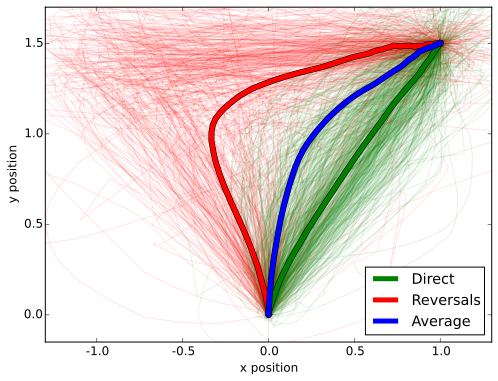
\includegraphics[width=\figurewidth]{imgs/exp2-average-cursor}
  \caption[The pitfalls of averaging cursor trajectories.]{
    \label{fig:average-cursor}
    Averaging direct trajectories (green) and reversals (red)
    produces an aggregate trajectory that appears to curve gently.
    However, few of the actual trajectories curve in this way.
    These data come from Experiment 2 (Chapter 3).
  }
\end{figure}


Again, though, the experiments reported here
reveal discrete movements towards one or other response option,
with reversals on some trials,
rather than the graded, curved trajectories seen in much previous work.
Therefore, an averaged trajectory is an inappropriate measure,
as it falls somewhere between the direct trajectories and the reversals
(see Figure~\ref{fig:average-cursor}).
For this reason, in Experiments 1 to 5
I instead code the location of the cursor over time on each trial
as being either on
the side of the screen corresponding to the correct option,
or the side corresponding to the foil
(excluding cases where the cursor is yet to be moved).
I then compared, in every 20 msec window,
the probability of being on either side of the screen to chance,
or the probability of being on one or other side between conditions,
using logistic mixed effects models (see below).
Attraction towards the foil option is therefore revealed by
an increase in the proportion of trials
where the cursor is on that side of the screen.

In line with previous mouse tracking studies,
for each time course analysis I run a series of comparisons,
one on each 20 msec time slice,
and report the times from which significant effects emerge and disappear.
Instead of t tests, however, I use logistic mixed models,
for reasons outlined below.

Finally, an alternative to running a series of comparisons
is to fit polynomial regression models, or \emph{growth curves},
to the time course data
(\citealp{Falke2013};
 \citealp[see][for an introduction to this method in eye tracking research]{Mirman2014}).
These are regression models in which time,
and often polynomial terms such as time$^2$ and time$^3$,
are included as predictors.
Such models are often used to model changes in subjects over time,
such as the change in height of a child over a number of months, hence their name.
Growth curves are discussed in detail in Chapter 6.




\section{Statistical Analyses}\label{sec:statistics}

Finally, I will use the remainder of this chapter
to outline some of the statistical methods used in this thesis.
Again, by covering this material here,
I hope to avoid repeating it throughout the later chapters.

\subsection{Mixed Effects Models}\label{subsec:statistics-lme}

Throughout this thesis, I use \emph{mixed effects} regression models
\citep{Gelman2007, Baayen2008}
--- otherwise known as linear or logistic mixed models (LMMs), hierarchical regression,
multilevel regression, and random effects regression ---
to analyse my data.
I will not provide a full tutorial on these methods here
\citep[see instead][]{Gelman2007, Baayen2008,Quene2008,Bates2015a}.
However, in this section I will explain my motivation in using these approaches,
and provide sufficient introduction so that readers
can follow the results presented later.
Unless otherwise stated, all analyses were conducted
using the R programming language \citep{RCoreTeam2015},
and mixed effects models were fit using the lme4 package \citep{Bates2015a}.

A typical psychology experiment records
several data points from each participant, one per trial.
For illustration, I will use the case of an experiment where
participants $p_1, p_2, ..., p_P$  perform a task in two conditions, $c_1$ and $c_2$,
and their response times $rt$ are recorded on each trial.
In a classical analyses, we would calculate the mean $rt$
for each participant in each condition,
and compare each participants' means from $c_1$
to those from $c_2$ using Student's t test.
Furthermore, there will be individual differences in $rt$ in general,
as some participants generally respond faster than others ---
this data is clustered within participants, in other words.
Therefore, we can improve our statistical power
by using a paired t test,
which accounts for these individual differences in baseline $rt$.

However, aggregating data in this way is not always appropriate
\citep[see][]{Baayen2008}.
Firstly, it discards a great deal of information,
and as a result the statistical power of our tests can be diminished.
Secondly, in averaging over multiple stimuli,
we ignore any systematic clustering by stimuli (or items) in our data:
some stimuli may produce faster responses than others in general, for example.
In linguistics, where items usually correspond to specific words or phrases,
this issue is traditionally addressed by running two analyses,
one aggregating by participant, and one by item,
and reporting the results of both \citep{Clark1973}.

A more serious problem with aggregation
is that it can involve unbalanced data.
In many analyses, we only include trials which meet certain criteria,
for instance only analysing response times for correct responses.
In reasoning research, where participants can often produce many different inferences,
this is particularly common.
If one participant gives few correct responses,
their average response time will be estimated from only a few trials,
and so will be a noisy measure.
In the classical analysis, however,
this datum is given as much weighting
as an average response time from a participant
who responded correctly on every trial.
When, as often is the case, there is some relationship between,
for instance, accuracy and response times,
this can cause systematic biases in our analysis,
hiding true effects and potentially creating spurious ones \citep{Baayen2008}.

Aggregation is also inappropriate
when the dependent variable is not a continuous quantity such as $rt$.
Most notably, when analysing proportions and percentages (e.g. accuracy),
aggregate data systematically violate the assumptions of t tests/ANOVA,
in a way which cannot be remedied by transforming the data \citep{Warton2010}.
These issues with aggregation can be avoided, however,
by fitting regression models to the data from each trial, rather than the aggregates.

As every undergraduate psychology student is taught,
the standard (unpaired) t test,
like the between-subjects ANOVA and many other classical tests,
is a special case of linear regression.
The regression equivalent of the unpaired t test for this experiment is given as

\begin{equation}
  \label{eq:lm1}
  rt_i = \alpha + \beta * Condition_i + \epsilon
\end{equation}

$rt_i$ is the $rt$ on trial $i$, and is the sum of
$\alpha$ (the mean $rt$ in baseline condition $c_1$),
$Condition_i$ (a dummy variable representing the condition on trial $i$,
set to $0$ to represent $c_1$ and $1$ to represent $c_2$),
$\beta$ (the difference in $rt$ between the conditions),
and the normally distributed error term $\epsilon$.

However, like the unpaired t test,
this model does not account for individual differences in $rt$.
To do this, we can extend Equation~\ref{eq:lm1}
so that the intercept $\alpha$ is allowed to differ for each participant.
This is, in effect, a within-subjects regression model.
The result is a \emph{mixed effects model},
in that it includes both \emph{fixed effects} ---
the overall intercept term $\alpha$,
and the overall effect of condition $\beta$ ---
and \emph{random effects} ---
the individual differences around $\alpha$.
Such a model is said to have \emph{random intercepts for each participant}.

Mixed models are even more flexible than this, however.
We may also want to allow for differences between each item in $rt$.
This can be done by including \emph{crossed random intercepts} \citep{Baayen2008}
for both participants and items,
allowing $\alpha$ to vary for each participant, and for each item,
while still calculating the overall intercept term.
These random effects are not restricted to the intercept either.
The $\beta$ term reflects the difference between the two conditions.
It may be that this difference is greater for some participants than others,
or greater for some items than others, if the same items are used in both conditions.
Therefore, we can also add random effects of condition for each participant,
for each condition, or for both, as desired.

\subsection{What Random Effects?}\label{subsec:statistics-random}

At this point, it should be noted that there is still active debate
as to what random effects should be included in a model.
\citet{Barr2013} argue for the use of \emph{maximal} random effects structures,
where random effects are included wherever the design of the experiment allows.
However, even with simple designs such a model cannot always be fit in practice,
as the amount of data required increases exponentially with the number of parameters to be fit.
Instead, \citet{Bates2015} advise using \emph{parsimonious} models ---
fitting the maximal model, and then removing the parameters
that account for least variation as necessary until the model can be fit.
It is this approach I have taken in this thesis,
and in each results section I specify the random effects structure used for the analysis.


\subsection{Data Transformations and Binary Outcomes}\label{subsec:statistics-tranform}

Being regression models, mixed effects models
can also make full use of the data transformations
and link functions used in regression modelling.
In this thesis, I use two such tools.
First, it is expected that latency data,
such as response times, movement initiation times,
and in Chapter 5, reading times,
will have a log-normal distribution:
a distribution like a normal distribution
that has been log-transformed.
Therefore, to analyse these measures I simply log-transform them,
and apply a standard linear mixed effects model.
Second, several of the measures I analyse,
including reasoning accuracy,
and the number of reversal trajectories per condition, are binary proportions.
These can be analysed by using logistic, rather than linear, mixed effects models.

\subsection{Categorical Predictors}\label{subsec:statistics-catgorical}


Just as the ANOVA is a special case of linear regression,
mixed effects models can be used
to evaluate the main effect of a categorical predictor
in these complex repeated-measures designs.
In the classical ANOVA, we use the Sum of Squares%
\footnote{More accurately, the sum of the squared deviations from the model fit.}
of models fitted with and without that predictor to  compute an F statistic,
which reflects the main effect of that predictor.
However, with mixed effects the degrees of freedom (DFs) for this F statistic
are not easily defined, and so it is difficult to calculate the appropriate p value.
In mixed effects models, we therefore compare
the deviance of models ($-2$ x their log-likelihoods)
fitted with and without the predictor,
and use a chi-squared test,
with DF corresponding to the number of terms added by larger model
(adding a categorical predictor with three levels adds 2 DF)
to find a p value for that predictor's main effect.

\subsection{Reporting}\label{subsec:statistics-reporting}

Of course, the output of mixed effects regression models
differs from that of a simple t test.
In most analyses, I will be investigating the effect of one or more
binary variables, such as condition, on the dependent variable.
This is quantified by the regression slope ($\beta$) for that variable,
and so for each comparison I will typically report
the means and standard deviations in each condition,
$\beta$ and its 95\% confidence intervals,
reflecting the estimated difference between the conditions,
and finally a t test comparing $\beta$ to 0.%
\footnote{
  In linear regression, the DF for this test
  would simply be the number of data points minus the number of variables.
  When random effects are included, it is not possible to define the DF in this way.
  In this thesis, I  take the conservative approach
  of using Satterthwaite’s approximation \citep{Satterthwaite1946} for the DF,
  as implemented in the lmerTest \citep{Kuznetsova2015} package for R.
  For logistic mixed models, the t test is replaced by a z test,
  and so it is not necessary to calculate DF.
}

For analyses where the dependent variable was log-transformed (e.g. response times),
the exponentiated regression weight $e^{\beta}$ is reported instead.
This indicates the percentage change in the dependent variable
between the conditions.
For instance, if the mean response time in condition $c_1$ is 1,000 msec,
and the effect of condition is $e^{\beta} = 110\%$,
response times in condition $c_2$ are
10\% greater than those of condition $c_1$, for an average of 1,100 msec.
$e^{\beta}$ is also reported for the logistic analyses,
where it reflects the multiplicative change in the odds of the outcome in question.
For example, if participants
gave the wrong response on 20\% of trials in condition $c_1$,
the odds ratio of wrong to right responses in this condition is $\frac{20\%}{80\%} = 0.25$.
An effect of $e^{\beta} = 1.5$ would mean
the odds were one and a half times greater of doing so in condition $c_2$;
odds of $0.25 * 1.5 = 0.375$,
which correspond to a probability of $\frac{0.375}{1 + 0.373} = 27.3\%$.


\chapter{Perceptual Similarity vs. Conceptual Knowledge in Induction}
\graphicspath{{3.Similarity/}}

\section{Introduction}

In Chapter 1, I discussed how people can
draw on different sources of information in induction.
In this chapter, I report a pair of experiments in which
two such sources --- perceptual similarity,
and conceptual knowledge in the form of category membership ---
are placed into conflict.
This was done using a mouse tracking version of
\citegap{Gelman1986}{'s} inductive triad task.
In Experiment 1, participants learned a biological property of
different species in the natural world, and were asked to
project each property to one of two species,
one of which belonged to the same taxonomic group as the base species.
In the conflict condition, but not the control condition,
the base and the foil species looked alike,
and so perceptual cues conflicted with conceptual knowledge.
In Experiment 2, participants completed a similar task,
but using artificial categories, learned at the start of the experiment.
I also manipulated the nature of the properties
participants reasoned about in Experiment 2, between participants,
to reveal how this modulated participants' inferences.

As discussed in Chapter 1,
theories of inductive reasoning can be organised into two groups.
One class of theory relies on conceptual knowledge
about the categories to which different entities belong,
and the relations between these categories.
Category membership is perhaps the most fundamental 
such form of conceptual knowledge that we can use as the basis for induction.
According to contemporary accounts of categorisation
\citep[see][]{Murphy2004,Rosch1988},
a category consists of a set of entities that have attributes in common.
Therefore, if we know the category to which something belongs,
we may believe that it has attributes
that we know are found in other members of that category
\citep{Murphy2004,Osherson1990}.
That adults can reason in this way has never been in question,
and indeed this idea is central to the very notion of categorisation
\citep{Mill1856,Gelman1986}.
This principle applies equally to inferences about people,
where it is better known as \emph{stereotyping}
\citep{Greenwald1995,Oakes1994}.
% The evidence that we do use knowledge about categories when reasoning
% is considerable, and indeed this should be self-evident,
% and so will not be reviewed in detail here.
% Few results in literature on inductive reasoning in adults
% \citep[see][for reviews]{Feeney2007,Hayes2010}, for example,
% can be accounted for without recourse to category-based inference.
Strikingly, people rely on categorical information
even when it is disadvantageous to do so.
Murphy and Ross \citep{Murphy2012,Murphy2010,Malt1995,Murphy1994}
showed, for instance, that when it is not certain
to which category an entity belongs,
participants nevertheless reason on the basis
of it belonging to the most likely category.
\citet{Mishra2010} also report a \emph{border bias} phenomena:
distant locations in the same state (for instance New York City, and Buffalo, New York) 
are perceived as physically closer, and more likely to share properties,
than closer locations divided by state lines (New York City and Princeton, New Jersey.

% \aside{I could also talk about language, and developmental trends here,
%   but I don't think I will}
Category membership is also at the core of many more sophisticated theories of induction
\citep[i.e.][]{Osherson1990,Griffiths2009,Kemp2009},
which combine information about category membership
with knowledge about the relationships between various categories.

% Similarity
Other theories of induction are not based on category membership.
Similarity between entities is the most common kind of
non-categorical information proposed to underlie induction:
entities that are similar (i.e. that share many features)
are more likely to also share a new feature
than things that are dissimilar.
This principle forms the basis of many feature-based accounts of induction
\citep{Sloman1993,Rogers2004,Sloutsky2004,Fisher2015},
discussed in Chapter 1.
\citet{Fisher2015} draw a distinction between two kinds of similarity,
based on either overlapping perceptual cues,
or on shared features in our mental representations.
With regard to adults' inferences,
the focus has been on the latter, \emph{representational} similarity.
While it is usually assumed that adults
are not swayed by inappropriate perceptual cues,
overlapping features in our mental representations of entities
form the basis of both \citegap{Sloman1993}{'s} Feature Based Induction model,
and \citegap{Rogers2004}{'s} Semantic Cognition accounts of induction.
\citet{Sloutsky2008,Sloutsky2004} propose
an analogous model to explain children's inferences,
based on perceptual similarity.
%% Interestingly, in contrast to findings \citep[i.e.][]{Murphy2012} that
%% reasoning under uncertainty is based on the most likely categorisation only,
%% inferences made under speeded conditions \citep{Chen2013,Verde2005,Newell2010}
%% are usually made on the basis of shared properties,
%% rather than category membership.

Given the importance of conceptual knowledge such as category membership in induction,
why then might perceptual similarity play a role?
One reason is that similarity is a useful proxy for shared category membership:
categories are collections of things that share properties, 
including visible features,
and things which look alike tend to belong to the same category.
Furthermore, regardless of category membership,
attributes tend to be correlated in the real world:
things that share properties we know of
are more likely to also share novel properties
\cite[see, e.g.,][]{Kemp2012}.
For both of these reasons, under many circumstances 
similarity --- even perceptual similarity ---
and conceptual knowledge will support the same inferences.
However, there do exist problems for which
these two kinds of information disagree,
most notably when reasoning about entities
that look more like members of a different category
than members of the category to which they belong
(that is, visually \emph{atypical} category members).
The archetypal examples of such atypical entities are whales,
which are mammals, but bear closer resemblance to fish
than to other mammals.


% Development
This chapter, like the rest of this thesis, focuses on adults' reasoning.
However, there has been little prior research on the role of
simple perceptual cues in adults' inductive reasoning,
perhaps because it would appear self-evident that
adults rely on conceptual knowledge,
or at least representational similarity.
There has been extensive debate, however,
as to whether young children make use of conceptual knowledge at all,
or if their inferences are simply driven by perceptual similarity.

There are a number of reasons to believe that children may rely on perceptual-cues,
rather than conceptual knowledge, in induction.
Conceptual knowledge must be acquired through instruction and experience,
and so early inferences, by which infants and children make sense of the world,
must be driven by a simpler, associative process like visual similarity
\citep{Westermann2013,French2004}.
In recent years, it has also become apparent that
simple associative mechanisms can produce
inferences that are surprisingly complex and flexible \citep{Sloutsky2008,Hinton2014}.
Indeed, \emph{deep neural networks} ---
neural networks, using simple associative principles but with many layers ---
are at the forefront of modern machine learning and artificial intelligence research
\citep{Mnih2013,Hinton2006}.

Sloutsky \citep[i.e.][see \citealp{Sloutsky2003,Sloutsky2010} for reviews]{
  Sloutsky2008,Sloutsky2007,Sloutsky2004a}
has therefore argued that young children's reasoning
is often based on such perceptual cues,
with reliance on conceptual knowledge arising later in development.
In contrast, Gelman 
\citep[i.e.][see \citealp{Gelman2011a,Gelman2004a} for reviews]{
  Gelman2013c,Rhodes2009,Gelman2007a,Gelman1986}
argues that even toddlers
 % \aside{Or younger?}
rely on conceptual knowledge about the world,
and naive theories \citep{Gopnik2003,Carey2009} 
to make inferences about the world around them.

\citegap{Gelman1986}{'s} triad task,
discussed in Chapter 1,
has been widely used as a testing ground
for these competing accounts.
Recall that in this task,
children were presented with images of two entities
(a flamingo and a bat, for instance),
given their labels (``bird'' and ``bat''),
and told a property of each
(``This bird's legs get cold at night'';
``This bat's legs stay warm at night'').
They were also shown a third species
(a blackbird in this example, labelled ``bird'',
but which more closely resembled the bat)
and asked to indicate which property it would have
(``Do this bird's legs get cold at night, like this bird's,
or stay warm at night, like this bat's?'').
\citet{Gelman1986} report that children as young as four
predominantly resist the perceptual cue,
and reason based on shared category membership --
projecting a property from the flamingo to the blackbird,
in this case.
On the other hand, \citet{Sloutsky2007} present results with artificial categories
that seem to show children ignoring category membership
in favour of perceptual similarity.
\citet{Gelman2013c}, however, demonstrate that
this result only holds under certain circumstances,
specifically, when the nature of the learned categories is obscure
and not obviously relevant to the properties being projected
(i.e. a creature's ratio of buttons to fingers).

% Hybrid theory
In Chapter 1, I introduced \citegap{Bright2014a}{'s} hybrid theory of induction.
This proposes that when reasoning inductively,
we can draw on either simple, associative knowledge --- such as similarity ---
or structured knowledge about the relationships between
entities and the categories they belong to.
The distinction in question in the current chapter,
between perceptual cues and simple conceptual knowledge,
is perhaps a more fundamental one than that made by
\citet{Bright2014a} between associative and structured knowledge.
Nevertheless, their hybrid account could easily
be extended to include it.

A prediction that emerges from this extended version of the hybrid theory
is that even adults' inferences may be influenced by perceptual similarity.
To date, there has been little evidence
suggesting that adults' inferences are driven by perceptual cues.
However, as discussed in Chapter 1,
this may in part be because methods used in previous work
were poorly suited to revealing such conflict,
and so in this chapter I explore this question
using the mouse tracking paradigm.
However, previous studies using this triad task
\citep[i.e.][]{Gelman1986,Sloutsky2007,Gelman2013c}
both with adult and child participants,
have only included trials in which perceptual similarity
and conceptual knowledge have conflicted.
Typically, adults overwhelmingly respond on the basis
of conceptual knowledge on such trials,
while the debate has focused on whether children's responses
are driven by conceptual knowledge \citep{Gelman1986,Gelman2013c}
or perceptual similarity \citep{Sloutsky2007}.
By not including trials in which both cues agree, however,
these experiments do not make it possible to see
if adults' reasoning was influenced by perceptual cues
in addition to conceptual knowledge:
when perceptual cues disagree with conceptual knowledge,
participants may be less likely to give the conceptually-cued response,
or slower to do so, or be otherwise conflicted,
than when the cues agree.

Therefore, in this chapter, I present two experiments, with adult participants,
in which perceptual cues either conflict or agree with conceptual knowledge.
If adult induction is in part driven by perceptual cues,
participants should be less likely to generalise
from a base entity to a conceptually-related one
when the alternative, foil entity is visually similar to the base.
Recording participants' mouse cursor trajectories,
it is also possible to investigate how these kinds of information interact over time.
If participants are driven by \emph{either} perceptual similarity
\emph{or} conceptual knowledge on each trial,
they should move the mouse directly to one or other response.
Alternatively, if participants are initially driven by
quickly-available perceptual cues,
but draw on conceptual knowledge later in the reasoning process,
we may see reversal trajectories, as participants
initially move towards the perceptually-cued option,
and change direction mid-trial.






\section{Experiment 1}

In Experiment 1, participants completed
a mouse tracking version of \citegap{Gelman1986}{'s} triad task,
with natural categories.
In the original version of this task, children had to choose
between generalising a property from a base species
to another conceptually-related species,
or to an unrelated but perceptually similar one.
This experiment is, to my knowledge,
the first to include a control condition,
in which both perceptual and conceptual information cue the same response.
Using this experimental manipulation, it is possible to
explore the role these perceptual cues play in reasoning.
Additionally, by recording participants' mouse cursor movements,
the experiment provides a window into processes during reasoning,
rather than just the final inferences participants make.



\subsection{Method}

\subsubsection{Participants}

Fifty nine undergraduate students took part in exchange for course credit.

\subsubsection{Stimuli \& Procedure}

At  the start of the experiment,
participants were presented with a framing story,
based on those used by \citet{Sloutsky2007} and \citet{Gelman2013c}.
This introduced a boy, Mark, who had moved to a country called Elbee,
where his teacher was teaching him
about the plants and animals found there.
They were instructed that they would be told
some of the facts that Mark's teacher had told him,
and shown pictures of three animals.
They were also instructed that their task was to decide,
given a fact about one species,
which of the two other species
this fact was likely to be true for.
This was illustrated using an example.

Participants then completed ten induction trials, in random order.
Induction stimuli were similar to those used by \citet{Gelman1986},
but were created for the current experiment.
They consisted of ten sets of species of plants and animals.
The full set of stimuli used can be found in Appendix~\ref{appendix:exp1_stimuli}.
Each set was made up of a \emph{base} species,
a \emph{correct response} species belonging to
the same super-ordinate category as the base,
and two \emph{foil} species, belonging to a different category:
one that was intended to be
perceptually similar to the base, and one that was not.
Each species was represented in the experiment
by a colour photograph (see Figure~\ref{fig:exp1-screenshot1},
and Appendix~\ref{appendix:exp1_stimuli}).
For each participant, five stimuli sets were randomly chosen as
conflict trials, and presented with the foil
that was perceptually similar to the base.
The remaining sets were designated control trials
and presented with the foil dissimilar to the base.

On each trial, the base was presented
in the centre of the screen,
with a property of that species shown above the image.
Blank genetic properties were used, of the form
``This one has gene 4ew. What else do you think has gene 4ew?''.
After clicking a button marked ``NEXT'' in the bottom centre of the screen,
images of the two possible response species
appeared in the top left and right corners,
with their positions randomised on each trial
(Figure~\ref{fig:exp1-screenshot1}).
Participants responded by clicking on one or other image,
and the position of the mouse cursor was recorded as they did so.

\begin{figure}[pt]
  \centering
  \includegraphics[width=.8\textwidth]{imgs/natural_conflict.png}
  \caption[Screen shot of conflict trial from Experiment 1.]{
    Screen shot of conflict trial from Experiment 1.
    The base image, a striped fish, belongs to the same category as the
    correct response option, the goldfish shown in the top left,
    but is perceptually similar to the foil option,
    the zebra in the top right.}
  \label{fig:exp1-screenshot1}
\end{figure}

\begin{figure}[pb]
  \centering
  \includegraphics[width=.7\textwidth]{imgs/exp1_posttest.png}
  \caption{Screen shot from the post-test check, Experiment 1.
    \label{fig:exp1-screenshot2}}
\end{figure}


After the reasoning trials, participants completed a post-test check.
This was to ensure that participants possessed the appropriate
structured knowledge about the relationships between
the species used.
Each base species was presented twice,
once alongside its corresponding correct response,
which belonged to the same biological category,
and once alongside its perceptually similar foil,
which did not.
The left-right positioning of these images
was randomised for each trial.
Participants were instructed to indicate
if each pair of species belonged to the same biological group.
% (Figure~\ref{fig:exp1-screenshot2})
The order of presentation of the post-test stimuli was totally randomised.


\subsection{Results}

On the post-test check,
for each stimuli set participants achieved at least 91\% accuracy
in correctly identifying that the base and correct response option
belonged to the same biological category,
and at least 68\% accuracy in correctly identifying that
the base and the foil option \emph{did not} belong to the same category
(binomial tests by participant, N = 59, p's < .0075;
minimum accuracy required for p < .01 is 40/59, or 67.8\%).
Post test scores for each stimulus set are included
in Appendix~\ref{appendix:exp1_posttest}.
Therefore, data from all stimulus sets
were included in the analyses.


I analysed the data using linear or logistic mixed models,
with random intercepts for each participant and each stimulus set,
and random coefficients for the effect of condition for each participant
(see Chapter 2).
Participants selected the foil species
on 4\% of trials in the control condition,
and 40\% of trials in the conflict condition;
$e^{\beta}$ = 209.1, CI = [3.6; 12169.2],
z = 2.577, p = .0100).
Therefore, perceptual similarity had a robust effect on their responses,
leading them to generalise the property to a foil species
belonging to a different biological group,
rather than to the base species,
considerably more often when the base and foil looked alike.


It is worthwhile assessing the pattern of individual differences in this effect.
Figure~\ref{fig:exp1_acc} shows the number of foil responses
each participant gave, by condition.
Forty nine participants were more likely to select the foil under conflict,
eight never selected it, and two showed the reverse effect, selecting the foil
less often under conflict.
Therefore, it appears that the effect of visual similarity
holds across almost all of the participants.

\begin{figure}[ht]
  \centering
  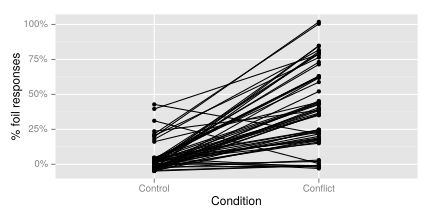
\includegraphics[width=\figurewidth]{imgs/exp1_acc.pdf}
  \caption{
    Proportion of foil responses given by each participant, per condition, in Experiment 1.
    \label{fig:exp1_acc} }
\end{figure}

The time taken to begin moving the mouse cursor (initiation time; IT),
and to select a response option (response time; RT)
both had positively-skewed distributions,
and so were log-transformed before analysis.
For correct responses,
there were no significant differences in IT between conditions,
taking 976 msec under conflict (SD = 1,000)
and 881 msec in the control condition (SD = 772; t = 0.104, p > .9).
However, RT was significantly slower
for conflict trials (2,668 msec, SD = 1,564)
than control trials (2,112 msec, SD = 1,279;
$e^{\beta}$ = 122.9\%, CI = [114.2\%; 132.3\%], t(58.5) = 5.553, p < .0001).

\begin{table}
  \centering
  \begin{tabular}{lrrrr}
    \toprule
    Condition & Response time & Initiation time & Reversals\\
    \midrule
    Control   & 2,112 (1,279) & 881 (772)       & 19\%\\
    Conflict  & 2,668 (1,564) & 976 (1,000)     & 43\%\\
    \midrule
    p         & < .0001      & > 0.9           & < .0001\\
    \bottomrule
  \end{tabular}
  \caption[Descriptive statistics for correct responses, Experiment 1.]{
    Summary statistics for correct responses in each condition.
    Standard deviations are shown in parentheses.
    Correct responses under conflict took significantly longer,
    and were more likely to be classed as \emph{reversals}.
    There was no difference in movement initiation times.
    }
\end{table}



Maximum Deviation (MD) % was also significantly higher
% for conflict trials (0.71, SD = 0.79)
% than for control trials (0.35, SD = 0.57;
% $\beta$ = 0.37, CI = [0.22; 0.51],
% t(54.0) = 5.128, p < .0001).
% However, MD
was bimodally distributed
(Bimodality Coefficient = .667;
Hartigan's D = 0.025, N = 453, p = .0058),
with trajectories either going directly to the selected response,
or moving towards one response, and changing direction mid-flight
(see Appendix~\ref{appendix:reversals}).
Trajectories were therefore classed as either \emph{direct} or \emph{reversals},
as described in Chapter 2.
When selecting the correct species,
participants were significantly more likely
to initially move towards the foil option
on conflict trials (37.7\%)
than on control trials (15.9\%;
$e^{\beta}$ = 4.8, CI = [2.5, 9.3], z = 4.699, p < .0001).

As discussed in Chapter 2,
there were therefore four kinds of mouse trajectories
observed in this experiment:
direct movements to the correct option (\emph{Direct Correct}),
initial movements towards the foil, which changed direction
to the correct option (\emph{Reversal Correct}),
initial movements towards the correct option, which changed direction
to the foil (\emph{Reversal Foil}),
and direct movements  to the foil (\emph{Direct Foil}).
Table~\ref{tbl:exp1_trajectories} shows how common
each trajectory type was in both conditions,
and indicates substantial increases in both incorrect responses
and reversal correct trials,
and a decrease in direct correct trials, under conflict.

\begin{table}
  \centering
  \begin{tabular}{lrrrr}
    \toprule
             & Direct Correct & Reversal Correct & Reversal Foil & Direct Foil\\
    \midrule
    Control  & 77.5\%         & 18.7\%           & 1.7\%         & 2.1\%\\
    Conflict & 34.4\%         & 25.8\%           & 8.2\%         & 31.6\%\\
    \bottomrule
  \end{tabular}
  \caption[Kinds of trajectory in Experiment 1.]{
    The four different possible kinds of cursor trajectory,
    broken down by condition.
    \label{tbl:exp1_trajectories}}
\end{table}

These different kinds of trial can be better understood
in terms of their \emph{transition probabilities} (see Chapter 2).
At the beginning of a trial, participants either move towards the correct option,
with probability $\alpha$, or towards the foil, with probability $1 - \alpha$.
After initial movement towards the correct option, they can either
select this option, with probability $\beta$, or the foil, with probability $1 - \beta$.
Finally, after moving towards the foil, participants can either
change direction and give the correct response,with probability $\gamma$,
or persevere and select the foil option, with probability $1 - \gamma$.
Figure~\ref{fig:exp1_transitions} shows
a schematic of these probabilities.
Table~\ref{tab:exp1_transitions_table}
show each of them across both conditions.
Again, these probabilities were compared using logistic mixed models,
with random intercepts for each stimulus set,
and random intercepts and slopes for each participant.

Participants were significantly more likely to
initially move towards the correct response in the control condition
(79\% of trials)
than the conflict condition (43\%;
regression $e^{\beta}$ = 7.3, CI = [4.7; 11.3], z = 8.773, p < .0001).
After doing so, they were also more likely to then select the correct response
in the control condition (98\%) than the conflict condition
(81\%; regression $e^{\beta}$ = 25.9, CI = [6.6, 101.2],
z = 3.078, p = .0021).\footnotemark
Finally, on trials where they did initially move towards the foil,
participants were more likely to eventually select the correct species
in the control condition (90\%)
than in the conflict condition (45\%;
regression $e^{\beta}$ = 26.6, CI = [7.0; 101.2], z = 4.815, p < .0001).

\begin{figure}[ht]
  \begin{floatrow}
    \ffigbox[.5\textwidth]{%
    \includegraphics[width=.5\textwidth]{../2.Methods/imgs/transitions.pdf}
    }{%
      \caption{
        The possible cursor transitions that can occur during a trial.
        \label{fig:exp1_transitions}
    }
    }
    \capbtabbox{%
      \centering
      \begin{tabular}{lrr}
        \toprule
        Parameter & Control & Conflict  \\
        \midrule
        $\alpha$  & 79\%    & 43\%$^{**}$\\
        $\beta$   & 98\%    & 81\%$^{**}$\\
        $\gamma$  & 90\%    & 45\%$^{**}$\\
        \bottomrule
        \multicolumn{3}{l}{
          \emph{Note}: $^{**}p < .01$.
        }
      \end{tabular}
      %% \begin{tabular}{cc} \hline
      %%   Author & Title \\ \hline
      %%   Knuth & The \TeX book \      Lamport & \LaTeX \\ \hline
      %% \end{tabular}
    }{%
      \caption{
        Transition probabilities for Experiment~1.
        \label{tab:exp1_transitions_table}
      }%
    }
  \end{floatrow}
\end{figure}


\footnotetext{
  As the value for the control condition was close to 1,
  regression parameters here would normally approach $\infty$,
  and the model would be unidentifiable,
  a phenomena known as \emph{perfect separation}
  \citep{Albert1984}.
  I therefore used penalised-likelihood estimation
  to impose an uninformative prior distribution \citep{Zorn2005}
  on the regression parameters, effectively reflecting a belief
  that when observed probabilities are close to 0 and 1,
  the true probabilities are likely to be higher, or lower, respectively.
  In this, and all future cases of perfect separation, I impose
  a Gaussian prior on the regression weights,
  with mean 0 and standard deviation 3.
}

Finally, if the processes drawing participants
towards selecting the foil on conflict trials operate early in reasoning,
we would expect movements towards this option to be initiated earlier
than those towards the correct species.
I found this to be the case,
with initial movements towards the foil initiated
after 687 msec on average (SD = 599),
and those towards the correct species initiated
after 1,182 msec (SD = 1,119).
Fitting a mixed model with random intercepts
for each participant and each stimulus set,
this difference was found to be significant;
$e^{\beta}$ = 130\%, CI = [120\%, 150\%], t(204.6) = 4.042, p < .001).


\subsubsection{Time course}

In order to investigate \emph{when} participants' mouse cursor movements
were drawn towards each response option,
I examined the position of the cursor over the first 4 seconds of each trial.
As participants largely moved discretely to one or other response,
these positions were not normally distributed,
and so I coded the location of the cursor
according to whether or not it was on the foil species' side of the screen.
By doing so, it is possible to identify at what points in time
participants' mouse movements are guided by perceptual similarity,
which drives participants towards selecting the foil species on conflict trials
(see Chapter 2).

\begin{figure}[tp]
  \centering
  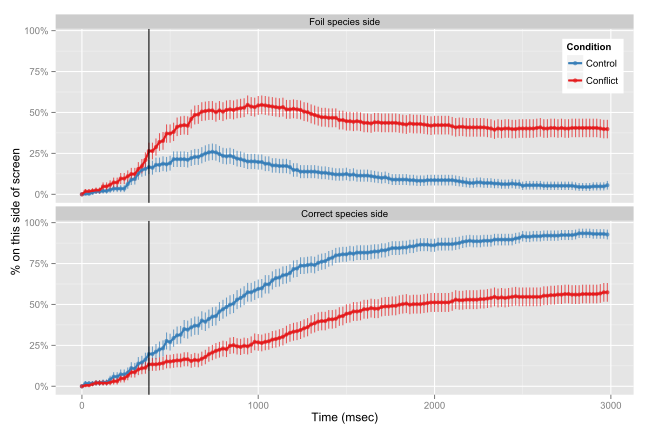
\includegraphics[width=.8\textwidth]{imgs/exp1_condition_timecourse.pdf}
  \caption[Time course, separately for each response option, in Experiment 1.]{
    Time course of attraction towards each response option.
    Vertical lines show the points from which
    the difference between the two conditions is
    statistically significant (p < .05).
    Error bars show 95\% confidence intervals.
    \label{fig:exp1_condition_timecourse}
  }
\end{figure}

\begin{figure}[bp]
  \centering
  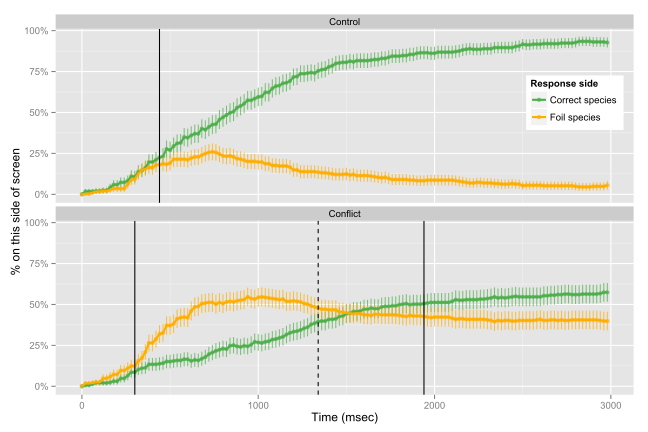
\includegraphics[width=.8\textwidth]{imgs/exp1_side_timecourse.pdf}
  \caption[Time course, separately for each condition, in Experiment 1.]{
    Time course of attraction towards each response option.
    Solid lines show the points from which one response
    is significantly more likely to be moved towards than the other (p < .05),
    while dashed lines for the points from which
    these differences are no longer significant.
    Error bars show 95\% confidence intervals.
    \label{fig:exp1_side_timecourse}
  }
\end{figure}

Figure~\ref{fig:exp1_condition_timecourse} shows the proportion of trials
on the side of the screen corresponding to each response option.
I fitted two series of logistic mixed models,
predicting the probability of being on the foil's side of the screen,
and one the probability of being on the correct species' side of the screen.
Each series consisted of a set of models,
one fitted to every 20 msec time window,
with condition as a predictor, 
and random intercepts for each participant, and each base species.
I used these series of models to find the divergence points:
the time from which participants were significantly more likely to move towards
the foil species in conflict trials than control trials,
and the time from which they were significantly more likely to move towards
the correct species in control trials than conflict trials.
In both cases, these significant differences between the conditions
emerged from 380 msec onwards.


Figure~\ref{fig:exp1_side_timecourse} shows
the same data, but with separate lines for each side of the screen,
and separate facets for each condition.
In the control condition, participants were significantly more likely
to move towards the correct option than the foil
from 440 msec onwards.
In the conflict condition, however, we see the interaction of
the two competing cues.
Participants were significantly more likely to move towards
the foil option from 300 msec.
This preference for the foil persisted until 1,340 msec,
at which stage both response options were equally popular.
From 1,940 msec, finally, participants were more likely to
move towards the correct option than the foil,
as the initial attraction towards the foil option
has been largely inhibited.
In other words, participants were
initially drawn towards the foil species on conflict trials,
but were later drawn towards the correct species instead.

\FloatBarrier




\subsection{Discussion}

This experiment placed perceptual similarity
and conceptual knowledge in conflict
in an inductive reasoning task.
My first goal in doing so was to test the prediction,
based on \citegap{Bright2014a}{'s} hybrid theory,
that adults' inferences would be influenced by perceptual cues,
as well as conceptual knowledge.
This prediction was confirmed by participants' responses:
when conceptual knowledge did not conflict with perceptual similarity,
participants selected the conceptually-cued response on almost every trial.
When the foil species looked similar to the base, however,
participants chose the foil 40\% of the time.
Additionally, this effect was found for the vast majority of participants,
and so is not the result of a few participants who are
inappropriately swayed by these visual cues.
When participants did give the correct response,
it appears that they experienced conflict
when perceptual cues supported the foil response,
taking significantly longer to respond,
and being more likely to initially move towards
the perceptually-cued foil option.

The mouse tracking paradigm makes it possible
to go beyond this finding, however,
and work towards a description of
how these two sources of information interacted during reasoning.
In Chapter 1, I raised two possibilities:
participants may either selectively use one or other cue,
or they may use perceptual cues by default,
but reject them in favour of conceptual knowledge
when they realise those cues to be inappropriate.
Consistent with both possibilities,
on control trials, where the base and the foil did not look alike,
participants initially moved towards the foil 21\% of the time.
On conflict trials, where they did look alike,
participants initially moved towards the foil 57\% of the time.
Furthermore, these movements %towards the foil under conflict
were initiated faster than movements towards the correct option in the same condition,
suggesting either
that conceptual knowledge takes longer to utilise than perceptual cues,
or that perceptual cues must be inhibited on these trials.

These two possibilities can be distinguished by looking to
what participants do when they have initially moved towards
a perceptually-cued foil.
In this situation, participants changed direction on 45\% of trials
to select the correct option instead.
By comparison, participants who initially moved towards the correct option under conflict
only changed direction to select the foil on 19\% of trials.
Therefore, it appears that, at least some of the time,
reasoning on the basis of conceptual knowledge required
the inhibition of the response based perceptual cues.
Together, these results suggest that perceptual cues
are used by default on this task.
By this view,  participants can either
initiate an early movement, driven by these cues (57\% of the time),
and subsequently either inhibit this response (45\% of the time),
or follow through with it and select the foil species.
Alternatively they can override these cues
before they move the cursor (43\% of the time),
and move directly towards the correct option.

Analysis of the time course data also appears to support this interpretation.
In Figure~\ref{fig:exp1_side_timecourse} we see that
on conflict trials, participants were initially (300 to 1,340 msec)
more likely to be on the foil side of the screen than the correct side.
By 1,940 msec, however, this trend had reversed,
and participants were instead more likely to be on the side of the correct option.

An interesting question, which this experiment does not answer,
is what factors dictate whether or not participants
moving towards the foil ultimately select this option,
or instead override this initial movement and select the correct species.
  %% In particular, a lot of recent Thompson/Pennycook work
  %% has looked at determinants of reflection from a DI perspective.
  %% Their account talks about metacognition, and Feeling of Rightness,
  %% in contrast to De Ney's intuitive conflict detection idea.
  %% For now, I'll just cite that work here, on the basis that
  %% the next draft of Ch1 will review it.}
This issue has come under increased scrutiny lately in the dual process literature
\citep[see, for instance,][]{Thompson2014a,Thompson2011,DeNeys2012,Pennycook2015},
where the focus has been on whether participants
reflect on their intuitive responses.
In the induction literature,
\citet{Gelman2013c} report a series of experiments with children
using the triad task.
They show that children are more likely to
use conceptual knowledge, rather than perceptual similarity,
when the conceptual categories used differed at a high, ontological level,
(animals versus robots),
than when they differed at a lower level (kinds of dogs, or creatures categorised
according to their ratio of fingers to chest buttons,
as used by \citealp{Sloutsky2007}).
They also demonstrated that children are more reliant
on conceptual knowledge when the properties under consideration
are meaningfully related to the different categories,
for instance animals being warm blooded, or robots containing batteries.
Both of these effects make sense from a normative perspective:
categories which are more conceptually distinct
provide a better basis for induction \citep{Rosch1976},
and certain kinds of category are conducive to
the projection of certain kinds of property,
for instance biological properties within biological categories
\citep{Heit1994,Shipley1993,Shafto2007}.
We would expect these same factors to influence adults' inferences.
However, it is not clear at what point in the reasoning process
such variables are important:
they may prompt reasoners to attempt
to draw on conceptual knowledge in the first place,
or they may cause them to be more likely to inhibit
their initial inappropriate perceptually-driven responses.

In Experiment 2, I presented participants with a version of this task
using artificial categories, specifically, a kind of animal, and a kind of robot.
I also manipulated, between participants,
the nature of the kind of properties being considered,
in order to investigate the effect this has on participants' reasoning.


\section{Experiment 2}


In Experiment 1, perceptual similarity drove participants' mouse movements
early in reasoning,
with conceptual knowledge being drawn on later in the process,
and in some cases overriding these perceptual cues.
In Experiment 2, I attempted to replicate these finding
using artificial categories --- a kind of animal, and a kind of robot ---
that participants learned in the laboratory.
I also manipulated, between participants,
the nature of the properties to be reasoned about,
to be either \emph{specific properties}, saliently related to the two categories ---
a robot having batteries, or an animal sleeping at night, for example ---
or fictional \emph{generic properties} --- such as being able to make a ``zevy sound''.
\citet{Gelman2013c} showed that children reasoning about specific properties
were more likely to draw on conceptual knowledge,
presumably as such properties make this knowledge more salient or accessible.
Here, this manipulation provides a window into how
perceptual cues and structured representations interact during this task.

\subsection{Method}

\subsubsection{Participants}

Forty eight participants completed the experiment for course credit.

\subsubsection{Stimuli \& Procedure}

Stimuli were adapted from drawings by \citet{LaRiccia2005}
used by \citet{Sussman2014},
and consisted of cartoon pictures of different kinds of creatures.
I created two categories:
animals called ``Flurps'',
and robots called ``Floobits''.
There were four possible body shapes,
and four possible colourations,
and each body shape and colouration was possible for both Flurps and Floobits
(Figure~\ref{fig:artificial},
see also Appendix~\ref{appendix:exp2_stimuli}).

Participants were again presented with a framing story about Mark,
who had just moved to Elbee,
but this time told that Mark was learning about
different kinds of things found outdoors there.
Two kinds of thing found in Elbee were presented,
animals called ``Flurps'', and robots called ``Floobits'',
designed to closely resemble Flurps.
Participants were told that both Flurps and Floobits
had different body types
and came in different colourations,
with the same body types and colourations found in both categories.
They were also informed that Flurps and Floobits could be
differentiated by looking at their heads:
Flurps had animal heads, with tentacles on top,
while Floobits had robotic heads
(see Figure~\ref{fig:artificial}).

After these instructions, participants completed eight categorisation trials,
with feedback,
in which they were presented with four Flurps, and four Floobits,
in a random order, and asked to categorise each.
These were intended to emphasise the distinction between the categories.
% \aside{I made a coding mistake here - I have each participants' response,
%   but not what stimulus they were responding to, so I can't
%   know they were accurate here. I'm pretty sure they understood the categories
%   though, both because reasoning performance was good,
%   and because all but 2 participants selected
%   one response on half the categorisation trials
%   and the other on the rest, like they would if categorising perfectly}
After the categorisation trials,
participants were told that for the final part of the experiment
they would be told a fact about one Flurp or Floobit,
and asked to decide which of two others
this fact was most likely to also be true for.
They were then presented with the sixteen induction trials, in random order.
Half of the participants reasoning about \emph{generic} properties
that were unrelated to the two categories
(i.e. ``This one can make a zevy sound'').
The remainder reasoned about \emph{informative} properties,
so that Flurps were presented with properties specific to animals
(``This one has a mummy''),
while Floobits were presented with robot-specific properties
(``This one has batteries inside'').
The full list of properties used can be found in
Appendix~\ref{appendix:exp2_properties}.

There were sixteen induction trials,
eight with Flurps as bases,
and eight with Floobits,
and the response options always consisted of
one Flurp and one Floobit.
Half of these were control trials,
in that the response entity belonging to
the same category as the base (the correct response)
was perceptually identical to the base,
having the same body type and colouration,
while the other, foil response entity was perceptually different,
with a different body type and colouration.
The remainder were conflict trials (Figure~\ref{fig:artificial}),
where the correct response was perceptually different from the base,
and the foil response was perceptually similar.

\begin{figure}[ht]
  \centering
  \includegraphics[width=\figurewidth]{imgs/artificial_screenshot.png}
  \caption[Screen shot from Experiment 2.]{
    A trial from Experiment 2.
    Participants were told that the \emph{Flurp} (centre)
    tries to stay warm, and asked to decide
    which of the other two things shown,
    the \emph{Floobit} on the left, or the Flurp on the right,
    also tries to stay warm.
    This is a conflict trial:
    the Floobit has the same colouration and body type as the base,
    but its robotic head identifies it as belonging to a different category.
    \label{fig:artificial}
  }
\end{figure}




\subsection{Results}

Unless otherwise specified,
I analysed the data using linear or logistic mixed models,
with random intercepts for each participant,
and random coefficients for the effect of condition for each participant.

Participants reasoning about generic properties
gave the foil response on
none of the control trials (N = 190),
but on 46\% of the conflict trials.
Those reasoning about specific properties
gave the foil response on 4\% of control trials,
and on 17\% of conflict trials
(see Table~\ref{tab:exp2_responses}).
A 2 (condition) x 2 (properties) logistic mixed model%
\footnote{
  Once again, as all participants gave the correct response
  in the control condition with generic properties,
  I used penalised maximum likelihood to set a normal prior,
  with mean 0 and SD 3, on the regression coefficients here \citep{Zorn2005}.
  This model also omitted the random coefficients
  for the effect of condition for each participant,
  due to convergence issues.
}
found a main effect of condition
($e^{\beta}$ = 95.7, CI = [28.6; 320.0],
z = 7.403, p < .0001),
and a condition x properties interaction
($e^{\beta}$ = 74.2, CI = [7.5; 730.4], z = 3.691, p < .0001),
such that the effect of condition was more pronounced
for participants reasoning about generic properties.

\begin{table}
  \centering
  \begin{tabular}{lrrr}
    \toprule
    \multicolumn{1}{l}{}          &
    \multicolumn{2}{l}{Condition} &
    \multicolumn{1}{l}{} \\
    \cmidrule(lr){2-4}
    Properties & Control & Conflict & Mean \\
    \midrule

    Specific   &    4\%  &    17\%  &  10\%  \\
    Generic    &    0\%  &    46\%  &  23\%   \\
    \midrule
    Mean       &    2\%  &    32\%  &        \\
    \bottomrule
  \end{tabular}
  \caption{
    Foil responses in Experiment 2.
    \label{tab:exp2_responses}
  }
\end{table}

Figure~\ref{fig:exp2_acc} shows how this effect was distributed across participants.
Recall that participants completed eight reasoning trials in each condition.
Of the 22 participants reasoning about generic properties,
16 were more likely to give the foil response under conflict,
none were more likely to do so on control trials,
and 8 never gave the foil response.
Of the 22 reasoning about specific properties,
11 were more likely to give the foil response under conflict,
2 more likely to do so on control trials,
and 11 never chose the foil option.
Therefore, as in Experiment 1, the main effect does not appear
to be driven by an effect only a subset of participants.

\begin{figure}[ht]
  \centering
  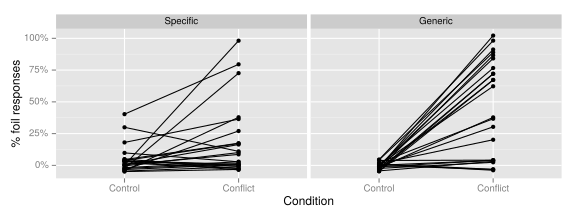
\includegraphics[width=\figurewidth]{imgs/exp2_acc.pdf}
  \caption[Proportion of foil responses given by each participant, per condition, in Experiment 2.]{
    Proportion of foil responses given by each participant per condition, in Experiment 2.
    separately for each property type.
    A small jitter has been added to vertical positions
    to show points which would otherwise overlap.
    \label{fig:exp2_acc} }
\end{figure}


\begin{table}
  \centering
  \begin{tabular}{llrrrr}
    %% Despace me!
   \toprule
    Properties                & Condition & Foil choices &  RT (msec)    & IT (msec) &  Reversals\\
    \midrule
    \multirow{2}{*}{Specific} & Control   &   4\%        &  1,366 (964)  & 377 (254) &  16\%\\
                              & Conflict  &   17\%       & 1,611 (1,162) & 362 (181) &  52\%\\
    \multirow{2}{*}{Generic}  & Control   &  0\%         &  1,547 (912)  & 444 (389) &  11\%\\
                              & Conflict  &   46\%       &  2,121 (1293) & 509 (576) &  59\%\\
    \bottomrule
  \end{tabular}
  \caption[Descriptive statistics for correct responses, Experiment 2.]{
    Summary statistics for correct responses, by property type and condition,
    on the odds of participants selecting the foil option (foil choices),
    and summary statistics for correct responses: response time (RT),
    movement initiation time (IT),
    and number of reversal trajectories (Reversals).
    \label{tab:exp2_descriptive}
  }
\end{table}


%% \begin{table}
%%   \centering
%%   \begin{tabular}{llllll}
%%     \toprule
%%                            & Foil choices & RT        & IT    &  Reversals\\
%%     \midrule
%%     Condition              & 95.7 ***     & 130\% *** & 102\% & 9.3 ***\\
%%     Properties             & 1.0          & 125\% **  & 114\% & 0.9\\
%%     Condition x Properties & 74.2 ***     & 119\% *   & 119\% & 1.7\\
%%     \bottomrule
%%     \multicolumn{5}{l}{ \emph{Note}: $^{*} p < .05;\ ^{**} p < .01;\ ^{***} p < .001;\ ^{****} p < .0001$ }
%%   \end{tabular}
%%   \caption{
%%     $e^{\beta}$ regression weights (odds ratio change for binary outcomes,
%%     and percentage change in log-transformed continuous outcomes,
%%     for main effects of condition and property type,
%%     and their interaction for each measure.
%%     Weights greater than 1/100\% indicate
%%     an increase in the dependent variable on conflict trials for the effect of condition,
%%     and increase for generic properties for the effect of properties,
%%     and an increase in the effect of condition when reasoning about generic properties
%%     for the interaction term.
%%   }
%% \end{table}

As in Experiment 1, IT did not differ significantly
between conditions or property types (p's > .2).
Response times were in general slower in the conflict condition (1,815 msec, SD = 1,239)
than the control condition (1,458 msec, SD = 941;
$e^{\beta}$ = 130\%, CI = [120\%; 140\%],
t(186.54) = 7.057, p < .0001),
and slower for generic properties (1,747 msec, SD = 1,094)
than specific properties (1478 msec, SD = 1,064;
$e^{\beta}$ = 125\%, CI = [106\%, 146\%],
t(46.1) = 2.731, p = .0089).
There was a significant condition x property interaction,
such that the effect of condition
was more pronounced for generic properties
($e^{\beta}$ = 119\%, CI = [103\%; 138\%],
t(186.4) = 2.382, p = .0182).

MD was bimodally distributed
(Bimodality coefficient = .635,
Hartigan's D = 0.02, p = .0341),
and so trajectories with MD greater than 0.747 were categorised as reversals
(see Appendix~\ref{appendix:reversals}).
For correct responses, these reversals occurred
significantly more often for conflict trials (61\% of trials)
than for control trials (17\% of trials;
$e^{\beta}$ = 9.2, CI = [6.0; 14.2], z = 10.21, p < .0001),
with no effect of property type, or condition x property interaction.

\begin{table}
  \centering
  \begin{tabular}{ll R{1.8cm} R{1.8cm} R{1.8cm} R{1.8cm} }
    \toprule
    Properties                & Condition & Direct Correct & Reversal Correct & Reversal Foil & Direct Foil\\
    \midrule
    \multirow{2}{*}{Specific} & Control   & 77.4\%         & 18.9\%           & 2.1\%         & 1.6\%\\
                              & Conflict  & 33.0\%         & 49.7\%           & 4.9\%         & 12.4\%\\
    \multirow{2}{*}{Generic}  & Control   & 85.8\%         & 14.2\%           & 0\%           & 0\%\\
                              & Conflict  & 20.6\%         & 33.3\%           & 12.2\%        & 33.9\%\\
    \bottomrule
  \end{tabular}
  \caption[Kinds of trajectory in Experiment 2.]{
    The prevalence of each kind of mouse trajectory, by condition and property type.
    \label{tbl:exp2_trajectories}}
\end{table}

There were therefore, once again, four kinds of cursor trajectories:
Direct Correct, Reversal Correct, Reversal Foil, and Direct Foil trajectories.
Table~\ref{tbl:exp2_trajectories} shows the proportion of each trajectory type,
broken down by condition and property type.
Across both property types,
participants were less likely to go straight to the correct option and choose it,
and more likely to do so for the foil option, under conflict.
In line with the analysis of reversals above,
initial movements towards the foil, which redirect to choose the correct option,
were more common under conflict,
and this difference was more pronounced for specific properties,
while this manipulation made participants reasoning about generic properties
more likely to instead give the foil response.



\begin{table}
  \centering
  \begin{tabular}{llccc}
    \toprule
    %%                        &            & \multicolumn{3}{c}{Parameter}\\
    Condition                    & Properties & $\alpha$             & $\beta$ & $\gamma$\\
    \midrule
    \multirow{3}{*}{Control}     & Specific   & 80\%                 & 97\%    & 92\%\\
                                 & Generic    & 86\%                 & 100\%   & 100\%\\
    \cmidrule(lr){2-5}
                                 & Both       & 83\%                 & 99\%    & 96\%\\
                              %% & Both       & \circled[blue]{83\%} & 99\%    & 96\%\\
    \midrule
    \multirow{3}{*}{Conflict}    & Specific   & 38\%                 & 87\%    & 80\%\\
                                 & Generic    & 33\%                 & 63\%    & 50\%\\
    %% \multirow{3}{*}{Conflict} & Specific   & 38\%                 & 87\%    & \circled{80\%}\\
    %%                           & Generic    & 33\%                 & 63\%    & \circled{50\%}\\
    \cmidrule(lr){2-5}
                                 & Both       & 35\%                 & 76\%    & 64\%\\
                              %% & Both       & \circled[blue]{35\%} & 76\%    & 64\%\\
    \bottomrule
  \end{tabular}
  \caption[Transition probabilities for Experiment 2.]{
    Transition probabilities for Experiment 2.
    Regardless of property type, participants are more likely
    to initially move towards the correct option ($\alpha$),
    and to ultimately select the correct option,
    either after initially moving towards it ($\beta$)
    or after initially moving towards the foil ($\gamma$)
    on control trials, where the correct option and the base look alike.
    On conflict trials, participants who initially moved towards the foil option
    were more likely to ultimately select the correct option instead ($\gamma$)
    when reasoning about specific properties than
    when reasoning about generic properties.
    Participants were initially less likely to move
    towards the correct option on conflict trials (blue),
    and after initially moving towards the foil on conflict trials,
    they were more likely to change direction and select the correct option
    if reasoning about specific properties than generic (red).
  }\label{tbl:exp2_transitions_table}
\end{table}


We can better understand these effects, once again,
by turning to the transition probabilities.
Table~\ref{tbl:exp2_transitions_table} shows
these transition probabilities,
broken down by condition and by property type.
I analysed these probabilities
using 2 (condition) x 2 (properties) logistic mixed models,
with random intercept terms for each participant.
Initial movements to the correct response,
with probability $\alpha$, were significantly more common for control trials (82.6\%)
than conflict trials (32.3\%;
$e^{\beta}$ = 10.1, CI = [7.0; 14.6], z = 2.312, p < .0001),
but with no main effect of property type.
A marginally significant condition x property interaction
($e^{\beta}$ = 2.0, CI = [0.9; 4.0], z = 1.904, p = .0569)
indicated that the effect of condition on $\alpha$
was slightly more pronounced for generic properties.

For trials where participants initially moved towards the correct option,%
\footnote{
  Again, in both the analysis of $\beta$ and $\gamma$,
  as means of 0 and 1 occurred in a number of cells,
  penalised maximum likelihood logistic regression was used,
  with a Gaussian prior (mean 0, SD 3) on each regression coefficient.
  }
the probability of ultimately selecting the correct option ($\beta$)
was greater in control trials (98.7\%) than conflict trials (75.8\%;
$e^{\beta}$ = 46.1, CI = [11.6; 182.9], z = 5.453, p < .0001).
There was no main effect of property type,
but there was a significant property x condition interaction
($e^{\beta}$ = 47.1, CI = [3.7; 601.5], z = 3.692, p = .0030),
such that the effect of condition for generic properties
was greater than that for specific properties.
It should be noted, however, that $\beta$ was largely positive.
Even on conflict trials, with generic properties,
participants who initially moved towards the correct option
ended up selecting in 63\% of the time.

For the trajectories that initially moved towards the foil,
the probability of changing direction and ultimately selecting the correct option ($\gamma$),
was lower for conflict trials (64\%)
than control trials (95\%;
$e^{\beta}$ = 34.4, CI = [7.1; 166.2], z = 4.402, p < .0001).
There was no main effect of property types, but
there was, crucially, a property x condition interaction
($e^{\beta}$ = 66.6, CI = [3.8; 1149.1], z = 2.890, p = .0039),
indicating that the effect of condition was greater
for participants reasoning about generic properties.
Post-hoc comparisons showed no difference
between participants reasoning about specific and generic properties
in the control condition ($\gamma$ > 92\%; $p_{adjusted}$ > .4),
but significantly more correct responses
after initially moving towards the foil option on conflict trials
when reasoning about specific properties (80\%)
than when reasoning about generic properties (50\%;
$e^{\beta} = 19.2, CI = [2.1, 174.5], z = 2.622, p_{adjusted} = .0088$.






In Experiment 1, I found that initial movements towards the foil option on conflict trials
were initiated more quickly than those towards the correct option.
Here, I fitted a 2 (initial movement direction) x 2 (property type) logistic mixed model,
with random intercepts for each participant and each base species,
and log-transformed initiation times from the conflict trials as the dependent variable.
There was a significant effect of initial direction,
such that movements towards the foil option (430 msec, SD = 527)
were again initiated faster than movements towards the correct option (558 msec, SD = 564;
$e^{\beta}$ = 118\%, CI = [1.07\%, 131\%], t(346.2) = 3.325, p = .0010).
There was no effect of property type, or condition by property interaction ($p's > .1$).


\subsubsection{Time course}

I repeated the time course analysis reported for Experiment 1,
looking at the proportion of trials on the side of the screen
corresponding to each response option over time.
Firstly, Figure~\ref{fig:exp2_foil_side_timecourse}
shows the proportion of trials on the side of the screen
containing the foil option, over time,
broken down by condition, and property type.
To infer when each variable began to influence participants' motor output,
I fitted a series of logistic mixed models,
predicting the proportion of responses on the foil side of the screen
at each 20 msec interval.
To test the effect of condition, I fitted models
with condition as a predictor, and random intercepts for each participant.
To investigate the effect of properties,
I fitted models with property as a predictor, and random intercepts for each participant,
to the data from conflict trials only,
as control trials were unaffected by manipulations of the property.
Participants were more likely to
move toward the foil option in conflict trials than control trials from 280 msec
(solid vertical line in Figure~\ref{fig:exp2_foil_side_timecourse}).
On conflict trials, participants reasoning about generic properties
were more likely to remain on the foil side of the screen than those 
reasoning about specific properties from 620 msec (dashed vertical lines).
In other words, participants reasoning about specific properties
were more likely to override their movement towards the foil from this point.


\begin{figure}[tp]
  \centering
  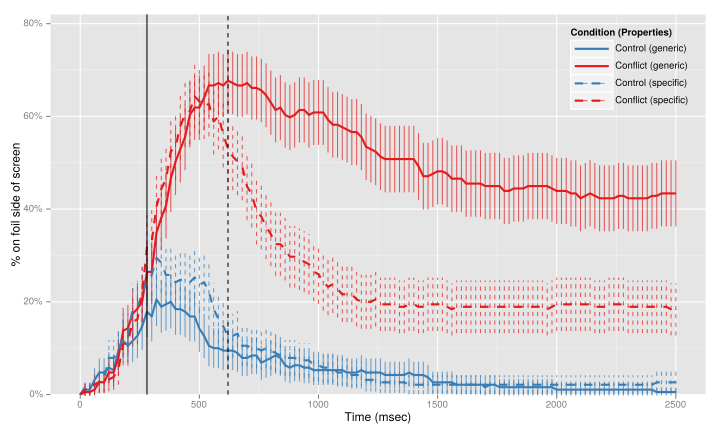
\includegraphics[width=\figurewidth]{imgs/exp2_foil_side_timecourse.pdf}
  \caption[Time course of attraction towards the foil, in Experiment 2.]{
    \label{fig:exp2_foil_side_timecourse}
    Proportion of trials on the side of the screen containing the foil option, over time.
    Participants were more drawn towards the foil option
    early in conflict trials (red) than control trials (blue)
    from  260 msec (solid vertical line).
    Later on conflict trials, participants were  more likely to remain on the foil side
    when reasoning about generic properties (solid red line)
    than specific properties (dashed red line),
    from 620 msec (dashed vertical line).
  }
\end{figure}

\begin{figure}[bp]
  \centering
  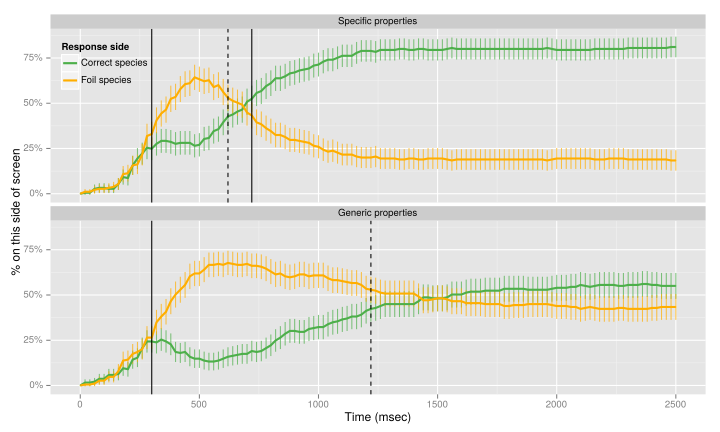
\includegraphics[width=\figurewidth]{imgs/exp2_conflict_timecourse.pdf}
  \caption[Time course for conflict trials, in Experiment 2.]{
    Time course of attraction towards foil and correct response options
    on conflict trials with generic (top) and specific (bottom) properties.
    Participants reasoning about both kinds of property
    show an early preference for the foil option
    (statistically significant from the first solid vertical lines to the dashed vertical lines)
    which is inhibited quickly for specific properties,
    and more slowly, and less often, for generic properties.
    Only participants reasoning about specific properties
    showed a later significant preference for the correct option (second solid vertical line).
    \label{fig:exp2_conflict_timecourse} }
\end{figure}

Figure~\ref{fig:exp2_conflict_timecourse} shows, for conflict trials,
the proportion of trials on the side of the screen corresponding to each response.
The top panel shows these trends for participants reasoning about specific properties.
Participants were significantly more likely to be on the side of the foil option than the correct option
from 300 msec (first solid vertical line) to 620 (vertical dashed line),
and subsequently significantly more likely to be on the side of the correct option
from 720 msec onwards (second solid vertical line).
The bottom panel, for participants reasoning about generic properties, shows a similar trend.
Participants were again significantly more likely to be on the side of the foil option
from 300 msec (first solid vertical line),
but this initial effect persevered for much longer when reasoning about generic properties,
to 1,220 msec (vertical dashed line),
and participants never showed a significant preference
for the correct option's side of the screen.

Therefore, participants reasoning about both kinds of property
were initially driven by perceptual cues in the conflict condition,
but those reasoning about specific properties
were more likely than those reasoning about generic properties
to subsequently draw on conceptual knowledge
and move instead to the side of the screen
containing the correct response option,
and were faster to do so.

\FloatBarrier



\subsection{Discussion}

In this experiment, participants completed 
a version of the inductive triad task using artificial categories.
Perceptual cues influenced both
participants' early cursor movements,
and their ultimate responses.
When perceptual cues and conceptual knowledge conflicted,
participants were more likely to initially move the cursor towards the foil option,
particularly if they were quick to initiate their movement,
and were also more likely to ultimately select the correct option,
regardless of initial movement.
Similarly, the time course data showed that
participants' cursor movements were driven by these perceptual cues
towards the foil option early on conflict trials,
but that this initial tendency was generally overridden.
In this sense, the current experiment
replicates the results of Experiment 1.

This experiment goes further by manipulating the kind of property
about which participants reasoned:
either specific properties, which were related to
the ontological distinction between the categories,
or uninformative, generic properties, which were not.
This manipulation had no significant effect
on participants' early movements,
and indeed in the control condition,
where participants rarely moved towards the foil option,
they appeared to play very little role at any stage.
In the conflict condition, however, where participants
initially moved towards the foil option on most trials,
I found that participants reasoning about specific, distinctive properties
were more likely to override their initial, perceptually-driven movement towards the foil
than participants reasoning about generic properties.
In other words, although reasoning about specific properties
made participants no less likely to initially rely on perceptual cues during reasoning,
it did make them more likely to reject their initial perceptually cued representation
(see Table~\ref{tbl:exp2_transitions_table}, and Figure~\ref{fig:exp2_conflict_timecourse}).



\section{General Discussion}


In these two experiments
participants completed versions of the inductive triad task
where they were asked to generalise a property from a base category
to one or other response category.
They could rely either on conceptual knowledge,
and so generalise the property to the category that
belonged to the same category as the base,
or on perceptual cues,
and generalise to the category that looked like the base.
In both experiments, I manipulated whether the cues agreed or disagreed,
so that on conflict trials perceptual cues would lead participants
to select the foil response option rather than the
conceptually-related one.
On these conflict trials, participants were
more likely to select the foil category.
Furthermore, they were more likely to make
fast initial mouse movements towards the foil,
which they often overrode to select the correct category instead.
These results are consistent with \citegap{Bright2014a}{'s} hybrid theory of induction.

I also raised the question of how perceptual cues
and conceptual knowledge might interact during induction.
One option was that participants
selectively relied on perceptual cues \emph{or} conceptual knowledge.
The alternative was that participants were
initially driven by perceptual cues,
but sometimes overrode theses cues when they realised them to be inappropriate,
and relied on conceptual knowledge instead.

The results showed that participants,
although usually initially moving towards the perceptually-cued foil,
sometimes moved directly towards the conceptually-cued option,
with these movements generally taking longer to initiate
than those towards the foil.
There are two possible explanations for such trials.
It may be that participants simply draw on conceptual knowledge here,
a process which takes longer, and then act on it.
Alternatively, participants on these trials
may have first processed the perceptual cues,
but inhibited them and replaced them with their conceptual knowledge
before initiating their cursor movement.
It is not clear at present how these possibilities could be disentangled,
and so for the time being this particular issue remains an open question.

In Experiment 2, I manipulated the kinds of properties participants reasoned about:
either specific properties, that were saliently related
to the distinction between the two categories,
or generic properties, that were not.
This manipulation mainly affected what participants did
on trials where they initially moved towards a perceptually-cued foil option.
Participants reasoning about specific properties were
significantly more likely to override their initial movement
and select the correct option instead
than those reasoning about generic properties.
The manipulation did not make participants any less likely
to initially move towards the foil option,
and its influence on the time course data
emerged relatively late in reasoning (see Figure~\ref{fig:exp2_foil_side_timecourse}).
It also had no influence on control trials,
where participants almost invariably selected the correct option.
Therefore, it would appear that this manipulation
mainly served to make participants more likely
to inhibit their perceptually-driven responses
on trials in which they were initially driven towards giving them.
This is consistent with much previous work,
both using the current paradigm \citep{Gelman2013c}
and other inductive tasks \citep{Heit1994,Ross1999},
indicating that the kind of information people draw on in inductive reasoning
is contingent on the nature of the properties to be projected.
A future question raised by this result concerns
whether this manipulation serves to make
participants more likely to inhibit perceptual cues,
or if it makes certain structured knowledge
easier to retrieve by cuing or priming it.

The purpose of these experiments
was to investigate adults' inductive reasoning,
and the results are consistent with \citegap{Bright2014a}{'s} hybrid account.
Specifically, they suggest that induction cannot be explained entirely
by either accounts based on unstructured associative knowledge
such as (perceptual or representational) similarity
\citep[i.e.][]{Sloman1993,Rogers2004,Sloutsky2004,Fisher2015}
or by purely structured, conceptual knowledge
\citep[i.e.][]{Osherson1990,Griffiths2009,Kemp2009,Gelman1986}.
Instead, both kinds of information appear to influence adults' reasoning,
with simple perceptual similarity drawn on earlier in the process,
and perhaps serving as a default.
However, these results also have implications for theories of children's reasoning.
As discussed in Chapter 1, and earlier in the current chapter,
a number of experiments have claimed to show that
young children's inferences are either
driven by conceptual knowledge
\citep{Gelman2013c,Rhodes2009,Gelman2007a,Gelman1986},
or that they are driven by perceptual similarity
\citep{Sloutsky2008,Sloutsky2007,Sloutsky2004a}.
These previous experiments \citep[i.e.][]{Gelman1986,Sloutsky2007,Gelman2013c},
however, have focused on a binary question:
do children draw on perceptual cues, \emph{or} on conceptual knowledge during reasoning?
Therefore, these experiments only presented participants with conflict trials,
and their responses were classed as either
consistent with reliance on perceptual similarity,
consistent with reliance on conceptual knowledge,
or not significantly different from chance in either direction.
As discussed in Chapter 1,
an experimental control condition, of the type used here,
where both cues agree, makes it possible to discover
not only which cue dominates when both conflict,
but also whether the neglected cue,
perceptual similarity in this case,
has any influence at all.

Therefore, these results with adults suggest a new interpretation
of the developmental data:
if both perceptual similarity and conceptual knowledge influence adults' reasoning,
they likely both also play a role in children's inferences.
This perspective may make sense of
apparently contradictory results in the developmental literature,
where children seem to draw on conceptual knowledge
in some scenarios but not others.
It is likely that these studies differ
in terms of the factors which make participants
more or less likely to inhibit initially influential perceptual cues.
Thus, while children may have access to both perceptual cues
and information about conceptual knowledge across all of these experiments,
they are more likely to inhibit the former in favour of the latter
when categories differ at a high, ontological level,
when entities are more easily categorised,
or when the properties under consideration are
conceptually related to the distinction between the categories
\citep{Gelman2013c}.
In short, the current results suggest that
developmental researchers should be less concerned
about \emph{whether} children rely on similarity or on conceptual knowledge,
and instead ask \emph{when} do children rely on either form of information.



% \aside{ This is where Newall 20 questions with nature bit comes in! }







% Having shown that perceptual and conceptual knowledge
% are activated during induction,
% our next question is how to these representations
% interact during the reasoning process.
% \aside{I need to look at trajectories when the wrong response was chosen.}
% Unlike a number of mouse tracking studies
% that found graded, continuous attraction towards both responses \citep[i.e.][]{Spivey2005},
% we found that participants moved directly towards one or other response,
% and on many trials moved initially towards one, before changing direction mid-flight.
% Earlier trajectories were more likely to be directed
% towards the perceptually-cued response option
% while later movements moved towards the conceptually-related option.
% This is consistent with the idea that only one representation
% can exist in working memory at a time.









\chapter{Associative vs. Structured Knowledge in Induction}
\graphicspath{{4.Associations/}}

\section{Introduction}

In Chapter 3, we saw that 
induction can be driven by more than one kind of information,
as perceptual similarity and conceptual knowledge
came into conflict during reasoning.
\citet{Bright2014a}, in their hybrid theory,
proposed a more subtle distinction in inductive reasoning,
between associative and structured knowledge.
While a number of results show that both kinds of knowledge
can drive inductive reasoning, however,
less is known about how these kinds of knowledge interact.
This is the question I seek to answer in this chapter.

As \citet{Bright2014a} note,
theories of induction can be classed in two ways.
Some theories propose that induction is based on structured knowledge:
the world is organised into coherent categories,
and specific knowledge about these categories,
and the often complex relationships between them,
is used as the basis for inference.
One such theory is \citegap{Osherson1990}{'s} similarity coverage model,
that describes inferences about species of animal
with reference to the taxonomic relationships between them.
More recent accounts have generalised this idea,
casting induction as a process of Bayesian inference
\citep{Griffiths2009,Griffiths2005,Heit1998,Kemp2009}.
At the core of these accounts is the notion that
in category-based induction,
we attempt to use the information given in the premises
(i.e. ``Carrots have disease X'')
to update our beliefs about the distribution of this property
across all categories.
To do so, we must be able to express how various categories are related:
the probability that rabbits have a given disease, given that carrots have it,
depends on the means by which diseases can be transmitted between various species,
in this case, through ecological interactions, such as a food chain.
Similarly, biological properties, such as genes,
are most strongly projected according to 
the distance between species in the taxonomic tree \citep{Heit1998,Osherson1990},
while if we know that certain artefacts are found in one city,
geographical distance is used to decide which other cities are likely to
house them \citep{Kemp2009}.

On the other hand,
a number of theories of inductive inference,
and category-based induction in particular,
rely on simpler, \emph{associative} forms of knowledge.
Similarity, including visual similarity,
discussed in Chapter 3, is one such form of knowledge;
things that are similar
\citep[share many properties, or features, that we know of; see][]{Medin1993}
are likely to also share novel properties.
For instance, on learning about two animals, both of which
live underwater, have scales, and breathe through gills,
we do not need to know what a ``fish'' is
to predict that if one lays eggs, the other likely does as well.
Of course, as discussed in Chapter 3, similarity comes in many forms,
and \citet{Fisher2015} make a useful distinction between
perceptual and representational (i.e. knowledge-based) similarity.
Perceptual similarity is most often proposed
as the basis of induction in children
\citep[][see also Chapter 3]{Sloutsky2010,Sloutsky2008,Sloutsky2007}.
A number of theories of induction in adults,
however, are based on the overlap of features
in our mental representations \citep{Rogers2004,Rogers2008,Sloman1993}
or perceptual input \citep{Sloutsky2008,Sloutsky2004}.
Other associative accounts of induction,
including of inductive generalisation during learning, are based on
what is variously referred to as contiguity, co-occurrence, or thematic relations:
things that are often seen together are more likely 
to share properties than things that are not
\citep{Kruschke1992,Rumelhart1986,Rescorla1972}.

% Also cited:
% Colunga & Smith, 2005;
% French, Mareschal, Mermillod, & Quinn, 2004; Jones & Smith, 2002; Sloutsky, Kloos, &
% Fisher, 2007).
% Smith and DeCoster (2000)

\citet{Bright2014a} argue that neither
structured nor associative accounts of induction alone are complete.
As noted by \citet{Murphy1985},
associative accounts of categorisation and induction
fail to capture some of the flexibility and complexity seen in human reasoning.
In particular, participants have been shown to be
sensitive to property effects when reasoning inductively:
the strength of an argument is dependent
on the kind of property projected
\citep{Heit1994,Shafto2007,Shafto2005}.
Therefore, transmittable properties such as infectious diseases
are thought to be shared by animals that are related ecologically,
such as predators and prey in a food chain,
whereas biological properties such as genes are shared 
only by animals that are close together in their taxonomic tree.
It is difficult to account for such flexibility in a purely associative account
\citep[but see work by][]{Sloutsky2008,Rogers2004}.
Structured models such as the Bayesian accounts discussed above \citep[i.e.][]{Kemp2009},
in contrast, draw on different knowledge structures for different inferences,
and so can capture this flexibility in human reasoning.

At the same time, it seems unlikely that 
structured knowledge alone drives inductive reasoning.
Induction is an ubiquitous phenomena, encompassing any inference that goes
``beyond the information given'' \citep{Bruner1973}.
This ranges from simple perceptual inferences,
to the development and postulation of scientific theories
\citep[see][for a taxonomy of inductive inferences]{Kemp2014}.
Furthermore, inductive reasoning is not exclusive to human adults:
similar inferences, although in simpler domains,
must be made both by children, and throughout the animal kingdom.
Associative theories of induction provide accounts that
make more reasonable claims about the cognitive abilities
required to reason inductively.
Indeed, in the spirit of \citet{Simon1956},
associative processes may \emph{satisfice},
often yielding the same inferences as structured accounts,
but with considerably less effort.

Faced with this dichotomy between associative and structured knowledge in induction,
\citet{Bright2014a} proposed a theory that combines both forms of knowledge.
This \emph{hybrid} theory claims
that both kinds of knowledge are drawn upon during reasoning,
with a key distinction between the two being their processing characteristics.
By this account, associative knowledge can be retrieved quickly and easily,
while structured knowledge is slower to retrieve,
and places greater demands on working memory to utilise.

Evidence for this hybrid theory
comes from experiments that manipulate 
the processing conditions under which participants reason.
This research is discussed in more detail in Chapter 1, but to recapitulate,
participants' inferences (their choices, or ratings of argument strength)
are predicted by measures of associative knowledge under all circumstances.
Furthermore, under favourable conditions only
(i.e. in the absence of time pressure, or cognitive load),
inferences are additionally predicted by
appropriate measures of structured knowledge,
such as whether participants believed two species
belonged to the same taxonomic group
when reasoning about biological properties.

Of particular relevance to this thesis, which focuses on \emph{conflict} in reasoning,
\citeauthor{Bright} (\citeyear{Bright}, see also \citealp[Chapter 5]{Crisp-Bright2010})
report a version of the inductive triad task \citep{Gelman1986}
that places associative and structured knowledge directly in conflict.
In the trial shown in Figure~\ref{fig:crisp_screenshot}, for example,
participants were told a biological property of carrots (they have ``C5s cells''),
and chose between generalising this property to rabbits, or to bamboo.
Carrots and rabbits are strongly associated,
and so a participant relying on associative knowledge
would project a property from carrots to rabbits.
This is despite the fact that the link between the species is a food chain,
and so doesn't provide a means for them to share a biological property.
Carrots and bamboo, on the other hand, are both plants,
and so are more likely to share such a property.
The associative link between the two species, however,
is substantially weaker, and so projecting the property to bamboo
requires that one inhibits the associative knowledge linking carrots and rabbits
before one can draw on the structured link between carrots and bamboo instead.
Consistent with the hybrid theory,
participants were less likely to select the
taxonomically-related response option
over a strongly associated foil in this task
when under heavy cognitive load,
or if they had poor semantic inhibitory control
\citep[a measure of their ability to inhibit
  task-irrelevant semantic information;][]{Markovits2004,Burgess1996a}.
Like most studies that analyse only participants' ultimate responses, however,
while these results do reveal what information drove participants' final choices,
we are limited in what conclusions we can draw about
how different processes interact during this task.
To address this shortcoming, in this chapter I present
a mouse tracking extension of the \citet{Bright} triad task.

\begin{figure}[ht]
  \centering
  \includegraphics[width=\figurewidth]{imgs/crisp_screenshot.png}
  \caption[A conflict trial from \citet{Bright}.]{
    A conflict trial from \citet{Bright}.
    Participants learn that carrots posses the given biological property,
    and asked which of the other two species, bamboo or rabbits,
    are likely to share this property.
    \label{fig:crisp_screenshot} }
\end{figure}


How might associative and structured knowledge interact during this task?
Again, I propose two possibilities.
First, it may be that people selectively draw on associative knowledge
\emph{or} structured knowledge for a given inference.
In this case, we would expect to find
little evidence of actual conflict during reasoning,
as both kinds of knowledge would not compete during a single trial.
This would lead to cursor trajectories where
participants move directly towards one or other option, and then select it,
rather than changing direction mid-flight.
The second possibility is that
associative knowledge may be activated early in reasoning,
but be later overridden, at least some of the time,
by slowly-retrieved, more cognitively demanding structured knowledge.
In this case, participants would be conflicted
when they do override, or at least attempt to override,
their association-driven response.
Cursor trajectories in this case should largely be
initially drawn to the foil species
when it is cued by associative knowledge,
but also likely to override this initial movement
and select the correct species instead
at least some of the time.





\section{Experiment 3}

In this experiment, I adapted \citegap{Bright}{'s}
inductive triad task to record participants' mouse cursor trajectories
as they choose to generalise a property to one or other species.
Analysing participants' responses, I hoped to replicate that study's %\citegap[, Chapter 5]{Crisp-Bright2010}{'s}
basic finding, that participants are less likely to select the taxonomically-related response species
when the foil option is strongly associated with the base species.
Going beyond this, however, I hoped to use participants'
mouse cursor data to draw conclusions about the processes leading up to these responses.

\subsection{Method}

\subsubsection{Participants}

Forty-one undergraduate students at Queen's University Belfast
participated in exchange for course credit.
Data were lost from one participant due to
a malfunction in the experimental software.
Participants completed the experiment in a laboratory.
The experiment was programmed using the PsychScript package
(see Chapter 2) and run in the web browser.

\subsubsection{Stimuli}

Stimuli were those used by \citet{Bright}.
There were fourteen experimental stimulus sets,
in which participants reasoned about genetic properties.
Each set consisted of a base species,
which participants were told had the property in question,
a correct response species, and two foil species.
Each species was represented in the experiment
by a labelled picture (see Figure~\ref{fig:exp3_screenshot}).
\citet[][Chapter 2]{Crisp-Bright2010} collected ratings of the strength of association
between the base and the correct species,
and between the base and strongly associated species.
She presented 18 undergraduate students
with pairs of species names (i.e. ``Snails and Octopuses'')
and asked them to rate, on a scale from 1 to 9,
how strongly associated they believed the species to be,
giving their first, intuitive response.
These average association ratings,
along with a table of the species used,
can be found in Appendix~\ref{appendix:exp3_associations}.

In each stimulus set, the base
and correct species were moderately associated with each other,
according to \citegap[, Chapter 2]{Crisp-Bright2010}{'s} ratings,
and belonged to the same taxonomic category
(mammals, reptiles, fish, birds, or plants).
The two possible foil species belonged to
a different taxonomic category than the base.
Each set had a conflict foil,
that was strongly associated with the base,
and a control foil, assumed to be weakly associated.
Each set was presented twice, once with its conflict foil,
and once with its control foil, for a total of twenty eight
experimental trials.
All stimuli used on experimental trials
can be found in Appendix~\ref{appendix:exp3_stimuli}

\begin{figure}[ht]
  \centering
  \includegraphics[width=\figurewidth]{imgs/exp3_screenshot.png}
  \caption[A screen shot from Experiment 3.]{\label{fig:exp3_screenshot}
    A screen shot from Experiment 3.
    Participants were told that the base species, Salmon,
    had a certain biological property,
    and where asked which of the two response species,
    Goldfish or Bears, were most likely to also have this property.
  }
\end{figure}

There were a further fourteen filler stimulus sets,
in which participants reasoned about diseases.
These consisted of the same base species as in the experimental sets,
but different response species:
the correct response species here were
the strongly associated foils from the experimental stimulus set,
and so related to the bases in a way
that would allow the transmission of disease,
while one foil response belonged to the same taxonomic group as the base,
and one did not.
Again, each set was presented twice, once with each foil.
These trials were included in order to prevent participants
from adopting a strategy of always selecting
the taxonomically-related response species,
and were not included in the analyses.
Participants were asked about genetic properties on experimental trials,
and diseases on filler trials.
Each property was given a fictional, uninformative name,
e.g. ``gene 5U3''/``disease 3k0''.






\subsubsection{Procedure}

The 28 experimental trials and 28 fillers were presented in randomised order.
Table~\ref{tab:exp3_procedure} shows the format of the reasoning trials.
Each trial began with the word ``GENE'' or ``DISEASE''
displayed in the centre of the screen in large font for 1 second,
and then shrinking and moving to the top of the screen
where it remained throughout the trials,
to remind participants what kind of property they were reasoning about.
Participants were next presented with the specific property
(text for filler trials in brackets):
``There's a kind of gene [disease] called x3f,
which is found in the body of [is known to infect] either...',
for 2.4 seconds.
They then saw one species option in
the top left corner of the screen,
along with the text ``...this species...'',
followed by the other species
in the top right corner
and the text ``...or this species'',
for 1.6 seconds each, with only one species shown at a time.
The location of each response option was randomised on each trial.
Both response options were then displayed,
along with the text
``Which species do you think is most likely to
have this gene in their bodies
[be infected by this disease],
given that it is also found in...
[that it also affects...]''.


\begin{table}[ht]
  \centering
  \caption{
    The procedure followed on reasoning trials
    in Experiments 3 and 4.
    \label{tab:exp3_procedure}
  }
  %% \doublespacing
  \begin{tabular}{p{.25\textwidth} p{.65\textwidth} p{.1\textwidth}}
    \toprule
    Stage & Stimuli & Duration (msec) \\
    \midrule
    Prime property &
    ``GENE'' or ``DISEASE'' in centre of screen &
    1,000\\[1cm]
    
    Property &
    ``There's a kind of gene [disease] called x3f, which is found in the body of [is known to infect] either \ldots{}'' &
    2,400\\[1cm]
    
    Response species \#1 &
    ``\ldots{}this species\ldots{}'' (show species in top left) &
    1,600\\[1cm]
    
    Response species \#2 &
    ``\ldots{}or this species.'' (show species in top right) &
    1,600\\[1cm]
    
    Prompt to start trial &
    ``Which species do you think is most likely to have this gene in their bodies [be infected by this disease], given that it is also found in\ldots{} [that it also affects\ldots{}]'' (show both response species, and ``Next'' button) &
    Click ``Next'' button\\[1cm]
    
    Show base species; Record response &
    Show base species in centre of screen; Record cursor position as participants select a response species. &
    < 5,000 \\
    \bottomrule
  \end{tabular}
\end{table}


At this point, participants were required to click a START button
in the bottom centre of the screen,
after which the text was replaced by a 1.5 second fixation,
and then by the base species.
After the onset of the base species,
participants responded by clicking one or other response species,
and the position of the mouse cursor was recorded continuously as they did so.
Participants were required to respond within 5 seconds,
and were prompted to start moving earlier
on trials in which the mouse cursor did not move
within the first 1.3 seconds,
a time which was selected based on pretests (see Chapter 2).
On trials in which participants moved
the cursor off the start button during the fixation period,
they were brought back to the point
before they clicked the START button,
and asked not to start moving
until they saw the final species.

Following \citet{Bright},
after the induction trials participants completed
a post-test check to ensure that they
possessed the appropriate structured knowledge.
For each experimental stimulus set,
the base species was paired with the correct response species
and both foil species, to create 42 pairs.
Participants were asked to indicate, for each pair,
if the two species belonged to the same ``biological group''.
There were also 42 filler questions,
created by pairing each base species
with its possible responses from the filler induction trials,
in which participants were asked if the pair
belonged to the same ``food chain''.
Each question was accompanied by the labelled images
of each species used in the induction trials,
and participants responded by clicking buttons
marked ``Yes'' or ``No''.
The 84 post-test questions were presented in random order.


\subsection{Results}

\subsubsection{Post Test Check}

The post-test data make it possible to ensure that participants
possessed the appropriate structured knowledge for each trial.
For instance, if participants did not realise that
dolphins and llamas belong to the same biological group (mammals)
then we cannot asses the interaction of
associative and structured knowledge when reasoning about these species.
Appendix~\ref{appendix:exp3_posttest} shows the proportion of participants
who correctly identified that the base and correct response species
belonged to the same taxonomic group,
and that the base and foil response species did not,
for the stimuli used in the experimental trials.
Participants only performed above chance on the post-test
for the correct response species for 7 of the 14 stimuli sets
(binomial test, N=40, 67.5\% accuracy required for p < .05),
and so only these sets were included in the subsequent analyses.

  
\subsubsection{Reasoning Accuracy}

Due to an error in the software used to run the experiment,
mouse cursor data were recorded incorrectly on 40 trials (7.1\% of total)
in which participants took more than 2,200 msec to respond,
and so these trials were discarded from the analysis.
In the analyses that follow, I fitted linear or logistic mixed models, 
with random intercepts for each participant, and for each stimulus set.

Participants were significantly more likely to
choose the foil species on conflict trials,
where the foil and the base were strongly associated (26\%),
than on control trials, where they were not (5\%;
$e^{\beta}$ = 10.6, CI = [5.2; 21.8],
z = 6.421, p < .0001).
It may be the case that this effect is driven by
a subset of participants who are influenced by associative knowledge.
Figure~\ref{fig:exp3_acc} shows each participant's number of foil responses, by condition.
Of the 40 participants, 30 gave the foil response more often under conflict,
none did so more often on control trials,
and 10 never gave the foil response.
Therefore, the main effect on participants' responses
appears to apply across all participants,
or at least all participants who did not achieve perfect accuracy.

\begin{figure}[ht]
  \centering
  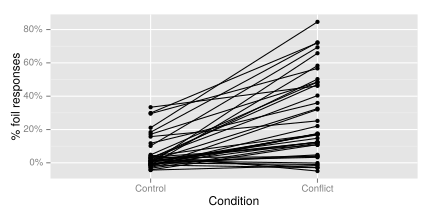
\includegraphics[width=\figurewidth]{imgs/exp3_acc.pdf}
  \caption[Participants' number of foil responses, by condition, Experiment 3.]{
    \label{fig:exp3_acc}
    Participants' number of foil responses, by condition.
    Of 40 participants, 30 gave more foil responses under conflict,
    and 10 never gave the foil response.
}
\end{figure}



\subsubsection{Correct Responses}

On trials in which the correct response was given,
there was no difference in response time between the conditions
(1,264 msec in conflict condition, SD = 297,
1,273 msec in control condition, SD = 361; t < .8, p > .4).
Participants were significantly faster to initiate the mouse movements
for correct responses in the conflict condition (628  msec, SD = 213)
than in the control condition (688 msec, SD = 206;
$e^{\beta}$ = 89\%, CI = [84\%, 95\%], t(405.2) = 3.670, p < .0001).

Maximum Deviation was bimodally distributed
(Bimodality Coefficient = .705; Hartigan's D = .0422, N = 520, p < .0001),
and trajectories were classified as either
direct trajectories or reversals, as described in Chapter 2 (MD cut-off = 0.524).
A significantly greater proportion of
trials where participants selected the correct species
were classed as reversals
in the conflict condition (16\%)
than the control condition (8\%;
$e^{\beta}$ = 2.2, CI = [1.2; 3.9], z = 2.524, p = .0116).
Therefore, although response latencies do not suggest conflict,
analysis of participants' mouse cursor movements shows that
responses based on structured knowledge
showed a greater attraction towards the foil response option
when the foil was strongly associated with the base species.

\subsubsection{Cursor Trajectories}

Once again, cursor trajectories in this experiment
can be classed as either
Direct Correct, Reversal Correct, Reversal Foil, or Direct Foil trajectories.
Table~\ref{tbl:exp3_trajectories} shows the proportion of
each trajectory type by condition.
Under conflict, there was a small increase in the number of
Reversal Correct responses,
and a considerably larger increase in the number of incorrect responses.

\begin{table}[h]
  \centering
    \caption[Kinds of trajectory in Experiment 3.]{
    \label{tbl:exp3_trajectories}
    Proportion of each trajectory type, by condition.
    Under conflict, participants were markedly more likely to 
    directly move to the foil option,
    and less likely to directly move to the correct option.
  }
  \begin{tabular}{lrrrr}
    \toprule
             & Direct Correct & Reversal Correct & Reversal Foil & Direct Foil\\
    \midrule
    Control  & 87\%           & 8\%              & 0.8\%         & 4\%\\
    Conflict & 62\%           & 12\%             & 3\%           & 23\%\\
    \bottomrule
  \end{tabular}
\end{table}


% |     &nbsp;     |   a   |   b    |   c    |
% |:--------------:|:-----:|:------:|:------:|
% |  **control**   | 88.2% | 99.09% | 32.2%  |
% |  **conflict**  | 64.7% | 95.83% | 66.01% |

Transition probabilities for trajectories from this experiment
are shown in Table~\ref{tab:exp3_transitions_table}.
Participants were significantly more likely to 
initially move towards the correct species on control trials (88\%)
than conflict trials (65\%;
$e^{\beta}$ = 4.7, CI = [2.9; 7.6], z = 6.284, p < .0001).
On trials where they have moved towards the correct option,
participants were also more likely to select it
on control trials (99\%) than conflict trials (96\%;
$e^{\beta}$ = 5.2, CI = [1.04; 26.2], z = 2.006, p = .0448),
although in both cases participants who initially move towards the correct option
are extremely unlikely to subsequently change direction.
Finally, on the trials where participants did initially move towards the foil option,
they are more likely to change direction
and select the correct option instead
on control trials (68\%)
than on conflict trials (34\%;
$e^{\beta}$ = 16.9, CI = [3.6, 80.2], z = 3.567, p = .0004).

Lastly, on conflict trials, movement initiation times
did not differ significantly between
initial movements that were towards the correct option (617 msec, SD = 225)
and those towards the foil option (652 msec, SD = 201;
t(251.8) = 1.365, p = .1733).

\begin{figure}[ht]
  \begin{floatrow}
    \ffigbox[.5\textwidth]{%
    \includegraphics[width=.5\textwidth]{../2.Methods/imgs/transitions.pdf}
    }{%
      \caption[The possible transitions that can occur during a trial.]{
        The possible transitions that can occur during a trial.
        \label{fig:exp3_transitions}
    }
    }
    \capbtabbox{%
      \centering
      \begin{tabular}{lPP}
        \toprule
        Parameter & Control & Conflict  \\
        \midrule
        $\alpha$  & 88\%    & 65\%^{***} \\ % p = 3.28e-10
        $\beta$   & 99\%    & 96\%^{*}   \\ % p = .044
        $\gamma$  & 68\%    & 34\%^{***} \\ % p = 0.00036
        \bottomrule
        \multicolumn{3}{l}{
          \emph{Note}: $^{*} p < .05;\ ^{**}p < .01;\ ^{***} p < .001.$
        }
      \end{tabular}
      %% \begin{tabular}{cc} \hline
      %%   Author & Title \\ \hline
      %%   Knuth & The \TeX book \      Lamport & \LaTeX \\ \hline
      %% \end{tabular}
    }{%
      \caption{
        Transition probabilities for Experiment~3.
        \label{tab:exp3_transitions_table}
      }%
    }
  \end{floatrow}
\end{figure}


\subsubsection{Time Course}

Figure~\ref{fig:exp3_condition_timecourse} plots
the proportion of trials in which the cursor is on
the foil species' side of the screen (top),
and the correct species' side (bottom),
broken down by condition.
For each plot, a series of logistic mixed models were fit,
with the probability of the cursor being on
that side of the screen predicted by condition (control or conflict),
across each 20 msec window, from 100 to 1,000 msec.
Random intercepts were included for each participant and for each base species.
By identifying the points from which
there were significant effects of condition in each series of models,
we can see at what point in time
manipulating the association of the foil species
affected participants' cursor trajectories
to that side of the screen.
Trials in the conflict condition were more likely to move towards
the foil response than those in the control condition from 480 msec onwards.
Those in the control condition were more likely to move towards
the correct response than those in the conflict condition from 760 msec onwards.

Figure~\ref{fig:exp3_side_timecourse} shows the same data,
but with separate plots for the control (top) and conflict (bottom) conditions,
and separate lines corresponding to the proportion of trials
on each side of the screen.
Divergence times were calculated in the same way,
this time reflecting the point, in each condition,
that participants became more likely to move towards
the correct species than the foil.
In both conditions, this divergence occurred at 480 msec.
This means that while participants selected the foil option
significantly more often on conflict trials than control trials,
they were no slower to show a preference for the correct species under conflict.

\begin{figure}[tp]
  \centering
  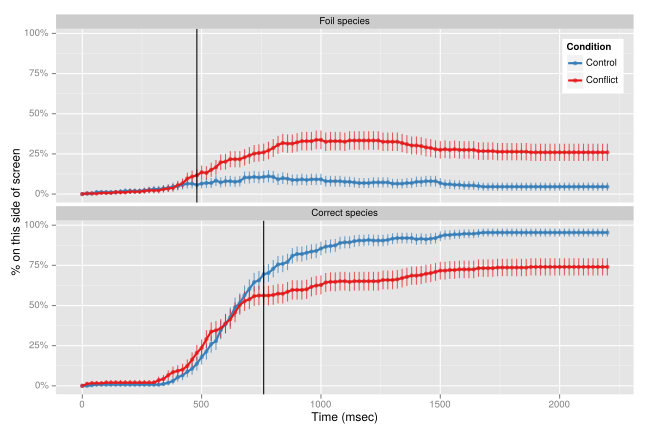
\includegraphics[width=.9\textwidth]{imgs/exp3_condition_timecourse.pdf}
  \caption[Time course, seperately for each condition, Experiment 3.]{
    Proportion of trials on each half of the screen, over time.
    Vertical lines show the points from which
    there were significant differences between
    the control and conflict conditions.
    \label{fig:exp3_condition_timecourse} }
\end{figure}

\begin{figure}[bp]
  \centering
  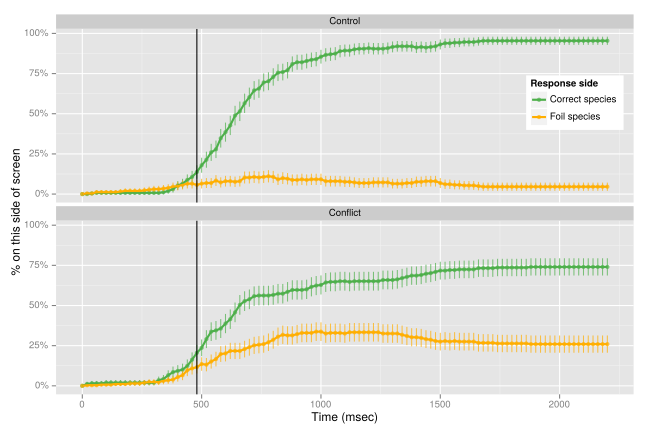
\includegraphics[width=.9\textwidth]{imgs/exp3_side_timecourse.pdf}
  \caption[Time course, seperately for each response option, Experiment 3.]{
    Proportion of cursors on each half of the screen, over time.
    Vertical lines show point from which participants were
    more likely to move towards the correct option
    than the foil.
    \label{fig:exp3_side_timecourse} }
\end{figure}

Recall that in Experiments 1 and 2,
the plots corresponding to the bottom panel of Figure~\ref{fig:exp3_side_timecourse}
showed a cross-over trend:
participants were initially more likely to move towards the foil option,
with this initial preference fading, and eventually reversing,
as the correct option was chosen on the majority of trials.
Here, instead, we see that participants 
are never more likely to move towards the foil option than the correct one.
The implications of these temporal dynamics are discussed below.



\subsection{Discussion}


 
In this experiment, participants had to generalise a biological property
from a base species to one of two other species:
one that belonged to the same taxonomic group as the base,
and one that did not.
On conflict trials, but not control trials,
there was a strong association between the base and foil,
so participants should have been drawn towards
selecting the foil species on these trials
if this irrelevant associative knowledge plays a role in inductive reasoning.
Replicating the core findings of \citet{Bright},
I found that participants were more likely to select the foil species
on conflict trials,
driven by associative knowledge.

Going beyond previous research, this experiment
allows us to draw inferences about how
these two kinds of knowledge interact.
\citet{Bright} also showed that
participants were more likely to select the foil response under conflict
if they had poor semantic inhibitory control,
or were placed under heavy cognitive load.
This suggests that drawing on the structured knowledge
needed to respond correctly on conflict trials
requires top-down executive functions.
It may be that the actual utilisation of structured knowledge
places demands on these executive processes, or alternatively,
that associative knowledge must be inhibited
before structured knowledge can be retrieved.
Perhaps consistent with the latter interpretation,
I found that on trials where participants did select the correct species,
they were more likely to initially move towards the foil species
on conflict trials, where the foil was strongly associated with the base.

Other findings, however, make this less clear.
The proportion of correct responses that were reversals, for instance,
was low compared to other experiments reported in this thesis:
8\% of control trials, and 16\% of conflict trials.
The current experiment also differed from Experiments 1 and 2
in that participants' response times were no slower
for conflict trials than for control trials.
Similarly, the participants initially moved towards
the foil species on only 35\% of conflict trials,
but after doing so, they only subsequently changed their minds
to select the correct species instead 34\% of the time.
Finally, the time course analysis showed that
even on conflict trials, participants never were more drawn
towards the foil species than the correct one.
Therefore, a more accurate description of these results is as follows.
In some cases participants' mouse movements
were initially driven by associative knowledge,
and later intervened upon on the basis of structured knowledge.
On the majority of conflict trials, however, participants either
moved directly to the species cued by structured knowledge,
or moved straight to the response cued by associative knowledge.

These results differ from those found in Experiments 1 and 2 in a number of ways.
However, before I attempt to interpret these results any further,
a limitation of this experiment must be noted.
Participants' performance on the post-test check,
which was used to ensure that they knew that
each correct response species belonged to the same biological group
as its corresponding base species, was extremely poor.
Specifically, participants' performance was not significantly above chance
when it came to knowing that the following species belonged to the same group:
dolphins and llamas,
monkeys and seals,
snails  and octopuses,
bananas and tulips,
penguins and chickens,
mice and goats,
and Orca whales and cows.
As a result, data from these 7 of the 14 stimuli sets
were excluded from the analysis.
Given that the purpose of this chapter is to study
conflict between associative and structured knowledge,
such poor taxonomic knowledge may be problematic.
Consider, for instance, 
a participant who is drawn towards 
generalising a gene from dolphins to cod,
rather than from dolphins to llamas.
If this participant knows that dolphins and llamas are mammals,
and cod are not, then we can infer that this attraction
is driven by unstructured associative knowledge.
However, if this participant believes that
dolphins and cod belong to the same taxonomic group,
then both their associative and structured knowledge
would support the same inference.
In this case, it is difficult to know what form of knowledge
they are drawing upon.

Therefore, In Experiment 4, I attempted to replicate these findings conceptually,
using new stimuli for which the appropriate taxonomic relationships are more obvious.
Furthermore, Experiment 3 relied on association ratings
collected by \citet[][Chapter 2]{Crisp-Bright2010}
from a different pool of university students,
and only allowed for the manipulation of the foil species,
which was either strongly associated with the base,
according to the prior ratings,
or (assumed to be) not associated.
In Experiment 4, in contrast,
I collected association ratings for each species pair
from each participant, after they had completed the rest of the experiment.
In this way, it was possible both to
investigate the relationship between association ratings
and participants' choices and cursor movements in a more nuanced way,
and to use each participants' actual beliefs about
the strength of association between species,
rather than aggregate ratings from a separate pool of participants,
in the analyses.


\section{Experiment 4}

In Experiment 4, I attempted to replicate the findings of Experiment 3,
but without the need to discard data from
trials for which participants lacked appropriate taxonomic knowledge.
Beyond this, I wished to explore
how each participants' own beliefs about the strength of association
between various species interacted with structured knowledge during reasoning.
Therefore, in this experiment, I asked participants to rate
the association between each base species
and every response species it was paired with for the reasoning trials.
This improves on the method used in the previous study in two ways.
First, while \citet[Chapter 2]{Crisp-Bright2010} collected
ratings of the association between the base species,
the correct response species, and the strongly associated foils used in the previous experiment,
she did not collect ratings for the associations between the bases
and the foil species assumed to be weakly associated.
Second, \citet{Crisp-Bright2010} collected
association ratings from one set of participants,
and reasoning data from another.
Therefore, it was the average association rating between species
that she used as a predictor in here analyses.
Here, on the other hand, I collected each participants'
own idiosyncratic ratings of the associations between the species,
allowing a more fine-grained analysis of
how such associative knowledge influences reasoning.


\subsection{Method}

\subsubsection{Participants}

Forty four undergraduate students completed the experiment
in exchange for course credit, in a laboratory.
The experiment was programmed using the OpenSesame experiment builder
(see Chapter 2).

\subsubsection{Stimuli}

In the experimental trials, participants were asked about
biological properties, specifically cells.
Nine new stimulus sets were generated for the experimental trials,
intended to be more familiar to participants
than those used in Experiment 3.
Each new set had three foil species,
one intended to be weakly, one moderately,
and one strongly associated with the base.
Each set was presented three times, once with each foil species.
Stimuli were selected according to a number of partial pretests,
in which participants rated the strength of association between species
using the procedure from \citet[][Chapter 2]{Crisp-Bright2010}, described above.
The full set of stimuli can be found in Appendix~\ref{appendix:exp4_stimuli}.

For the filler trials, where participants were asked about diseases,
an additional fourteen stimulus sets were generated,
each containing a base species,
a correct response species likely to share a disease with the base,
and three different foil responses, one for each time the set was presented.
One possible concern about the design of Experiment 3
is that the species designated as the correct response
for each experimental stimulus set
was the correct response on every trial it featured in.
Therefore, the fourteen correct response species from the experimental trials here
were used as foil species (that is, the species that
were unlikely to share a disease with the base species)
on three different filler trials.
This meant that these species were the correct response option
in the three experimental trials in which they featured,
but also the incorrect response option in three filler trials.
The properties to be reasoned about ---
genes on the experimental trials,
and diseases on filler trials~---
were unchanged from Experiment 3.

To ensure that participants did not complete
experimental trials with the same base species in close succession,
the order of trials was randomised with constraints for each participant.
First, the experimental trials were randomly divided
into three blocks of nine trials,
with each block containing
three weak, three moderate, and three strong foils,
and one trial from each stimulus set in each.
Nine of the twenty-seven filler trials were then added to each block.
Finally, the order of trials within each block was randomised repeatedly,
until at least 5 trials separated repetitions of each base species.

\subsubsection{Procedure}

There were minimal changes to the reasoning trials from Experiment 3.
However, this experiment was conducted using the OpenSesame platform,
which allowed greater experimental control over the mouse cursor.
Therefore, instead of requiring participants
not to move the cursor during the fixation period,
the cursor's position was automatically reset
to the centre of the START button after the fixation.

After the reasoning trials, participants again completed a post-test check.
In the first part of the post-test, participants rated the strength of association
of the thirty-six base-response species pairs from the experimental trials.
These consisted of the nine base species,
each of which was paired with its correct response species
and its three foil species.
For this section, participants were presented with the following instructions,
taken directly from  \citet[][Chapter 2, p. 60]{Crisp-Bright2010}:

\begin{quote}
  [...] Please think about all kinds of possible associations, such as causal,
  functional, categorical, etcetera. Please do not think in detail about
  the mechanism by which they are related, just give your intuitive
  response. For example, if you believe that ladybirds and butterflies
  are strongly associated please give a rating closer to 9. In contrast,
  if you think cars and ladybirds are unrelated, please give a rating
  closer to 1. Please give the answer that first comes to mind, as fast
  as possible.  
\end{quote}

On each rating trial, the labelled images of each species
were shown side by side, with their positions randomised.
Participants gave their ratings by clicking on buttons
labelled 1 to 9 below the images,
with 1 subtitled ``Not associated at all'',
and 9 subtitled ``Very strongly associated''.

The second part of the post-test checked participants' structured knowledge.
Participants were presented with pairs of species,
in the same format as the association rating trials,
and gave yes or no responses by clicking the marked buttons.
There were three blocks in this part of the post-test,
and the order of trials within each block was randomised.
First, for each of the nine experimental stimulus sets,
the base species and the correct response species
belonged to the same taxonomic group.
These nine pairs of species were presented along with
an additional nine pairs that did not belong to the same group.
Participants were asked in each case if the pair shown
belonged to the same \emph{biological group}, and told
``Biological groups are the main branches
when you think about the `family tree' of the natural world'',
and that the biological groups in the experiment were
mammals, fish, reptiles, birds, and plants.

Second, for five of the experimental stimulus sets,
the base species was related to the moderately and strongly associated foils
via a food chain relationship --- one species eats the other.
These ten base-foil pairs were presented along with
ten other species pairs not related in this way.
Participants were asked if each pair shown belonged to the same \emph{food chain},
and told ``Species belong to the same food chain if one is eaten by the other
(predators and prey for animals, or a plant which is eaten by an animal)''.

Finally, for the remaining four experimental stimulus sets,
the base species was related to the moderate and strong foils
in that they shared an ecological habitat.%
\footnote{
  This was not technically true for penguins and arctic wolves,
  and penguins and polar bears, as these species live in
  opposite polar regions, but the post-test data showed that
  participants do not realise this.
}
These eight base-foil pairs were presented along with
the eight other pairs that did not share a habitat,
and participants were asked if thee pair shown ``live in the same kind of habitat''.



%%% Local Variables: ***

\subsection{Results}

\subsubsection{Post Test Check}

For each stimulus set used in the experiment,
participants correctly said that the base species
and the correct response species 
belonged to the same taxonomic group (accuracy > 70.5\%, p's < .01),
and that the moderate and strong foils
had the appropriate relationship (food chain or shared habitat)
with their base species (accuracy > 75\%, p's < .001).
Therefore, no data were excluded from the analyses on these criteria.
Full post-test results can be found in Appendix~\ref{appendix:exp4_posttest}.

\subsubsection{Reasoning Accuracy}

In order to analyse data from the reasoning trials,
for each trial I divided that participants' rating of
the association between the base and the correct species
by their rating of the association between the base and the foil.
This produced a ratio reflecting the extent to which
that participants' associative knowledge
favoured one or other response option.
Values of this ratio ranged from $\frac{1}{9}$
($.111$; association of 1 for the correct species, and 9 for the foil),
to $\frac{1}{1}$ (equal association for both species),
to $\frac{9}{1}$
(association of 9 for the correct species, and 1 for the foil).

For each analysis, I log-transformed this ratio
to create a normally-distributed linear predictor,
as is standard practice when using ratios as regression predictors \citep{Gelman2007}.
Note that $log(\frac{1}{1}) = 0$,
and correspondingly $log(\frac{>1}{1}) > 0$ and $log(\frac{1}{>1}) < 0$
(see Figure~\ref{fig:exp4_log_transform}).
Therefore, when using the log-transformed ratio as a predictor,
a positive regression weight means that
the dependent variable is greater/more likely when the ratio is greater than $\frac{1}{1}$,
or in other words, when the association rating favours the correct response.

\begin{figure}[h]
  \centering
  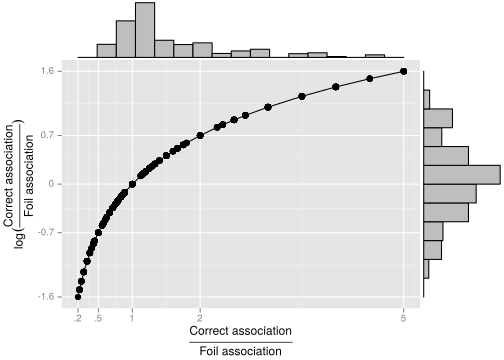
\includegraphics[width=.7\textwidth]{imgs/exp4_log_transform.pdf}
  \caption[The log-transformed association ratio, used as a predictor in Experiment 4.]{
    To analyse data from Experiment 4,
    each participants' rating for the association between
    the base species and the correct response species
    was divided by their rating for
    the base and the foil species, to form an association ratio.
    These ratios were log-transformed to use as predictors in regression analyses:
    after log-transformation, the difference between 1 and 0.2 (dividing by five)
    is the same as the difference between 1 and 5 (multiplying by five).
    \label{fig:exp4_log_transform}
  }
\end{figure}

Some aspects of the analyses based on this ratio are slightly unusual,
and so I will go through my first analysis,
predicting participants' responses,
in detail to familiarise readers with the method.
Figure~\ref{fig:exp4_ratio_accuracy} plots the proportion of correct responses 
(choosing the species belonging to the same taxonomic group as the base) given, on the y axis,
as a function of the association ratio, on the x axis.
Note that the x axis is log-scaled.
For plotting, I have divided the log-transformed ratio into 13 equal bins,
and plotted the mean and standard error of the dependent variable within each bin.
For the analyses, I fit log-linear, or logistic mixed models,
with random intercepts for each participant, and for each stimulus set.
The log-transformed association ratio from each trial was used as the predictor in the models.

\begin{figure}[h]
  \centering
  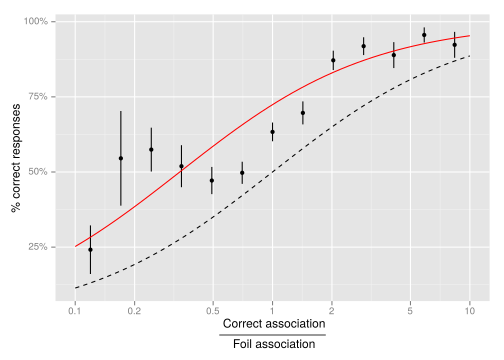
\includegraphics[width=.6\textwidth]{imgs/exp4_ratio_accuracy.pdf}
  \caption[Effect of the association ratio of participants' accuracy, Experiment 4.]{
    Correct responses on Experiment 4, as a function of
    the association ratio in favour of the correct species.
    As the ratio increased in favour of the correct species,
    participants became more likely to select that species.
    The fitted model (red line) included a significant positive intercept term,
    meaning that participants were more likely to select the correct species
    than would be predicted based on the association ratio alone (dashed black line).
    \label{fig:exp4_ratio_accuracy}
  }
\end{figure}

The association ratio was a significant predictor of the odds of a correct response
($\beta$ = 0.89, CI = [0.68, 1.1], z = 8.604, p < .0001).
Interpretation of the regression $\beta$ here is not straightforward,
but positive $\beta$s indicate that the dependent variable
(odds of a correct response) was positively related to
the size of the association ratio in favour of the correct response.
Fortunately, we can simply look to the predicted values from this model
(solid red line in Figure~\ref{fig:exp4_ratio_accuracy})
to see the magnitude of this effect.

An unusual property of these models is that
the intercept parameter is also meaningful.
As the log-transformed association ratio is the only predictor in the model,
the intercept reflects the expected value
when this predictor is at 0, or in other words, for a ratio of $\frac{1}{1}$.
If participants do not make use of structured knowledge,
we would expect participants to select the correct species
50\% of the time for such trials, something that would correspond to an intercept of 0.
The dashed black line in Figure~\ref{fig:exp4_ratio_accuracy}
shows the predicted values for such a model, with intercept 0.
A significant positive intercept means that
participants were more likely to select the correct species
than would be expected from the association ratio alone,
while a negative intercept means they were less likely.
There was a significant positive intercept term in this model
($logit(\beta)$ = 72\%, CI = [56\%, 85\%], z = 2.585, p = .0010).
I report the $logit$ of the regression $\beta$ weights here
as an easily interpretable measure of how much participants
were biased towards the correct species.
In this case, $logit(\beta)$ reflects how often
participants would be expected to select the correct species
on trials where the association ratio = $\frac{1}{1}$,
according to the fitted model
(i.e. where the red line on Figure~\ref{fig:exp4_ratio_accuracy}
crosses $1$ on the x axis).
Together, these results mean that participants were
a) more likely to select the correct species when
they rated it as being more strongly associated with the base
than the foil was, and
b) biased towards the correct option rather than the foil
beyond the effect of the association ratio.

\begin{figure}[h]
  \centering
  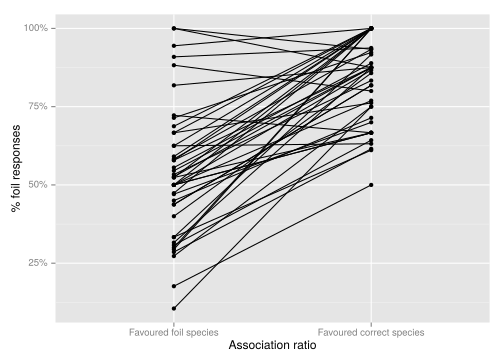
\includegraphics[width=.7\textwidth]{imgs/exp4_acc_ids.pdf}
  \caption[Proportion of correct responses
    given by each participant, by association ratio,
    in Experiment 4]{
    Participants' number of correct responses
    on trials where the association ratio favoured either
    the correct species or the foil species.
    40 of 44 participants were more likely to select the correct species
    when the association ratio favoured it
    than when the ratio favoured the foil.
    \label{fig:exp4_acc_ids} }
\end{figure}

To analyse individual differences in the number of correct responses
(Figure~\ref{fig:exp4_acc_ids}),
I calculated the number of correct responses given by each participant
both when the association ratio favoured the foil species,
and when it favoured the correct species,
excluding trials where species were rated as equally associated.
Of the 44 participants, 40 were more likely to select the correct species
when the association ratio favoured it,
and 4 were less likely to do so.
Therefore, it appears that almost all of my participants
were influenced by the association between species.

\FloatBarrier
\subsubsection{Correct Responses}

Analysing trials where the correct species was selected,
the association ratio had no effect on participants' movement initiation times
(mean = 574 msec, SD = 285; t(529.6) = 0.387, p > .6).
There was a marginally significant effect of the association ratio
on participants' response latencies
(mean RT = 1509, SD = 567;
$e^{\beta}$ = 98\%, CI = [96\%, 100.4\%], t(787.1) = 1.647, p =.100),
meaning that participants were marginally faster to respond correctly
as the association ratio in favour of the correct species increased.

Maximum deviation was once again bimodally distributed
(Bimodality Coefficient = .635; Hartigan's D = .025, N = 1188, p < .0001),
and reversal trajectories were classified
as described in Chapter 2 (MD cut-off = 0.923, see Appendix~\ref{appendix:reversals}).
Figure~\ref{fig:exp4_reversals} shows the proportion of correct responses
that were categorised as reversals ---
that is, where participants moved initially towards the foil
before selecting the correct species ---
as a function of the association ratio.
A logistic mixed model (dashed red line) showed that
participants were less likely to follow such a reversal trajectory
as the association ratio increased in favour of the correct species
($e^{\beta}$ = .8, CI = [.6, .97], z = 2.152, p = .0314).
However, the data were fit slightly better%
\footnote{
  As these two models were not nested,
  and contained the same number of parameters,
  we can identify which model best fits the data
  by comparing the deviance of each,
  but we cannot calculate p values for
  the difference between the models.
}
($\Delta$deviance = $0.715$)
by an alternative model (solid red line),
where the odds of a trajectory being classed as a reversal
when selecting the correct species
were predicted by the \emph{absolute magnitude} of the log-transformed association ratios
($e^{\beta}$ = .7, CI = [.5, .9], z = 2.289, p = .0221).
In other words, when selecting the correct species,
participants were most likely to trace a reversal trajectory
when the species were equally associated,
and less likely to do so as the ratio changed in favour of either species.
This trend may appear counter-intuitive,
but may make sense when one considers that
this analysis does not include trials where the foil species was selected.
An explanation for the trend is offered in the discussion, below.


\subsubsection{Cursor Trajectories}


As before, mouse trajectories in this experiment
can be described in terms of whether or not
they initially moved towards the correct species ($\alpha$),
whether they selected the correct species
after initially moving towards it ($\beta$),
and whether they changed direction to select the correct species
after initially moving towards the foil ($\gamma$;
see Figure~\ref{fig:exp3_transitions}).
I modelled these three parameters
using multilevel logistic regression models,
with the log-transformed association ratio
and an intercept term as predictors,
and random intercepts for each participant and stimulus set.

\begin{figure}[tp]
  \centering
  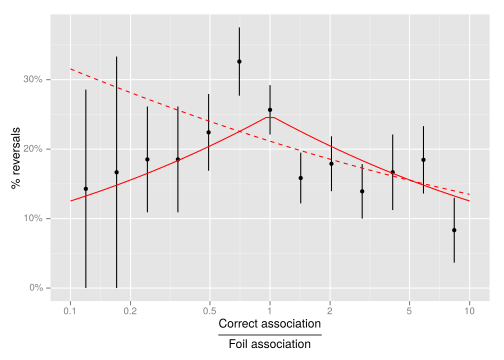
\includegraphics[width=.7\textwidth]{imgs/exp4_reversals.pdf}
  \caption[Proportion of correct responses that involved reversals,
  Experiment 4.]{
    The proportion of correct responses
    where participants initially moved towards the foil species.
    A model using the log-transformed association ratio as a predictor
    (dashed red line) showed that participants were more likely
    to produce these reversal trajectories when the association ratio
    favoured the foil species.
    However, the data were slightly better fit by a model (solid red line)
    which showed that these reversals were most likely to occur
    when the association ratio favoured neither response.
    \label{fig:exp4_reversals}
  }
\end{figure}

\begin{figure}[bp]
  \centering
  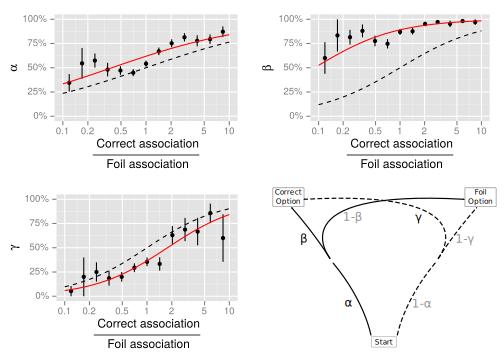
\includegraphics[width=.7\textwidth]{imgs/exp4_transitions_combined.pdf}
  \caption[Transition probabilities, as a function of the association ratio,
    in Experiment 4.]{
    \label{fig:exp4_transitions}
    Transitions probabilities from Experiment 4,
    as functions of the association ratios.
    As the association ratio increased in favour of the correct species,
    participants became more likely to initially move towards that species ($\alpha$, top left),
    to select that species after initially moving towards it ($\beta$, top right),
    and to select it even after initially moving towards the foil ($\gamma$, bottom left).
    Dashed lines show the expected values if participants were
    influenced by association ratio only.
    Overview of the three parameters can be seen in the bottom right.
  }
\end{figure}


The model for $\alpha$ (Figure~\ref{fig:exp4_transitions}, top left)
had a marginally significant positive intercept
($logit(\beta)$ = 62\%, CI = [50\%, 73\%], z = 1.886, p = .0593)
indicating that participants initially moved towards the correct species
on 62\% of trials when the ratio was $\frac{1}{1}$,
more than the 50\% that would be expected 
based on the association ratio alone.
The association ratio was also a significant positive predictor
($e^{\beta}$ = 1.7, CI = [1.4, 2.0], z = 6.109, p < .0001)
such that participants became more likely to initially move
towards the correct species as it was increasingly favoured by the association ratio.

The model for $\beta$  (Figure~\ref{fig:exp4_transitions}, top right)
had a robust positive intercept
($logit(\beta)$ = 80\%, CI = [85\%, 92\%], z = 10.567, p < .0001),
meaning that after initially moving towards the correct species,
participants selected that species 80\% of the time
when the association ratio was $\frac{1}{1}$.
The association ratio was also a significant positive predictor here
($e^{\beta}$ = 2.4, CI = [1.8, 3.2], z = 5.678, p < .0001),
meaning that participants became more likely to select the correct species
on trials where they initially moved towards it
as the association ratio in favour of the correct species increased.
In general, however, participants very rarely
changed direction after moving towards the correct species
in any case.

Finally, the model for $\gamma$  (Figure~\ref{fig:exp4_transitions}, bottom left)
contained a significant \emph{negative} intercept
($logit(\beta)$ = 37\%, CI = [30\%, 43\%], z = 3.963, p < .0001),
indicating that on trials where they initially moved towards the foil species,
participants only changed direction to select the correct species instead
37\% of the time when the association ratio was $\frac{1}{1}$.
The association ratio was again a positive predictor here
($e^{\beta}$ = 2.6, CI = [2.0, 3.5], z = 6.374, p < .0001),
meaning that as the strength of the association ratio
in favour of the correct species increased,
participants were more likely to switch direction
and select the correct species when they initially moved towards the foil.


\subsubsection{Time course}
\FloatBarrier

\begin{figure}[ht]
  \centering
  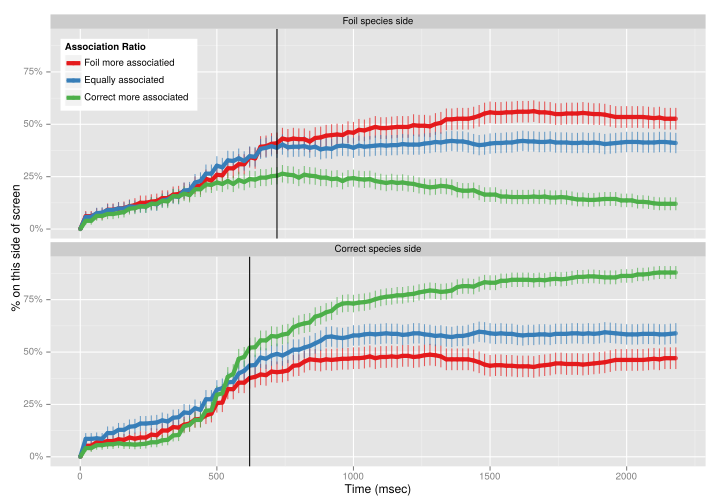
\includegraphics[width=\figurewidth]{imgs/exp4_condition_timecourse.pdf}
  \caption[Time course, separately for each response option, in Experiment 4.]{
    Proportion of trials on side of screen corresponding to the correct species (top)
    and the foil species (bottom) over time.
    The association ratio is a significant predictor
    of movements towards the foil from 720 msec,
    and of movements towards the correct species from 620 msec (solid vertical lines).
    \label{fig:exp4_condition_timecourse} }
\end{figure}


As usual, the time course of  the mouse movements here
reveals more about the points at which participants were
drawn towards each response.
Figure~\ref{fig:exp4_condition_timecourse} shows the proportion of trials
on the side of the screen corresponding to each species over time,
for trials where the association ratio favours the foil species (N = 359),
the two species were rated as equally associated (N = 397),
or the correct species was more strongly associated (N = 432).
To estimate divergence times,
I fitted two series of logistic mixed models,
one series predicting the probability of being on the foil species' side of the screen,
and one the probability of being on the correct species' side,
separately for every 20 msec time window.
Each model included the log-transformed association ratio  as a predictor,
and included random intercepts for each participant and each base species.
The divergence points were the times in each series
after which the association ratio is found to be a significant predictor.
The association ratio had a significant effect on
participants' probability of being on the foil species'
side of the screen from 720 msec,
and their probability of being on the correct species' side from 620 msec.

\begin{figure}[h]
  \centering
  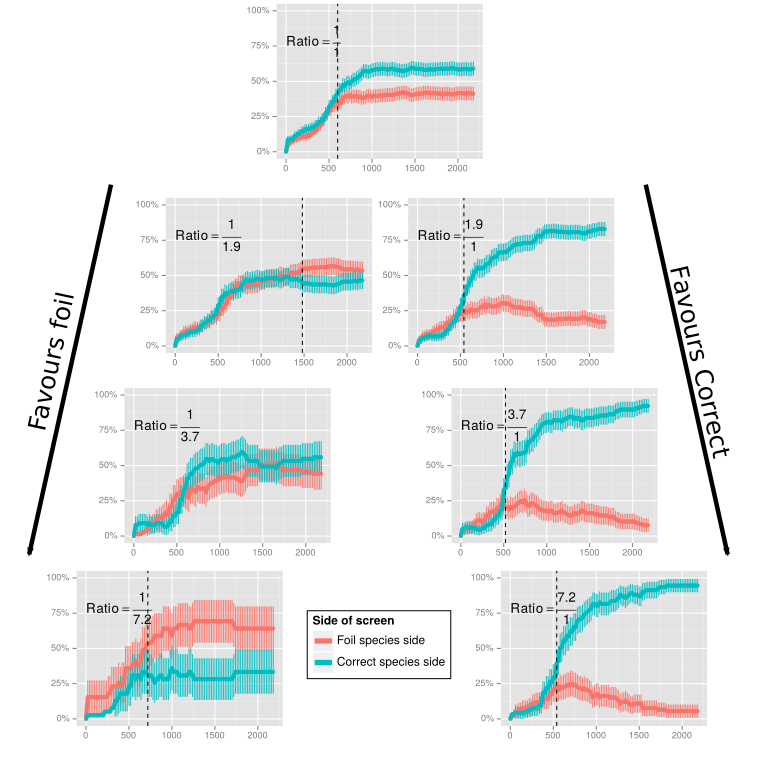
\includegraphics[width=\figurewidth]{imgs/exp4_ratio_timecourse.pdf}
  \caption[Time course, separately for different association ratios, in Experiment 4.]{
    Proportion of trials on the side of the screen corresponding to each response,
    grouped by association ratios.
    When the association ratio favours the correct option,
    %% \aside{This figure should have the divergence points marked for each trial,
    %%   a legend somewhere, and the font sizes all the same.
    %%   I will do this in the next few days when I've the use of a computer with a mouse.}
    \label{fig:exp4_ratio_timecourse} }
\end{figure}

\begin{table}
  \centering
  \caption[Divergence times, Experiment 4.]{
    Divergence times, and number of trials included,
    for each binned value of the association ratio.
    For ratios of $\frac{1}{7.2}$ and $\frac{1}{1.9}$,
    participants were significantly more likely to be on
    the foil species' side of the screen than the correct species'
    from the divergence time onwards.
    For all other ratios, participants were more likely to be on
    the correct species' side of the screen
    from the divergence time.
    \label{tab:exp4_ratio_timecourse_table}
  }
  \doublespacing
  \begin{tabular}{lrr}
    \toprule
    Ratio           & Divergence (msec) & N\\
    \midrule
    $\frac{1}{7.2}$ & 720               & 39\\
    $\frac{1}{3.7}$ & N/A               & 77\\
    $\frac{1}{1.9}$ & 1,480              & 243\\
    $\frac{1}{1}$   & 600               & 397\\
    $\frac{1.9}{1}$ & 540               & 223\\
    $\frac{3.7}{1}$ & 520               & 117\\
    $\frac{7.2}{1}$ & 540               & 92\\
    \bottomrule
  \end{tabular}
\end{table}

Figure~\ref{fig:exp4_ratio_timecourse}
shows the proportion of trials on either side of the screen,
with separate plots representing different levels of the association ratio.
For this analysis, I divided the log-transformed association ratio
into seven bins of equal width,
and labelled each bin according to the mean association ratio within it:
$\frac{1}{7.2}$, $\frac{1}{3.7}$, $\frac{1}{1.9}$, $\frac{1}{1}$, $  \frac{1.9}{1}$, $\frac{3.7}{1}$, and $\frac{7.2}{1}$.
Within each of these bins, I found the divergence point,
after which participants were more likely to be
on one side of the screen than the other,
by fitting a series of logistic mixed models,
comparing the probability of being on either side of the screen,
with random intercepts for each participant and each base species.

As the association ratio in favour of the correct species increased,
from $\frac{1}{1}$ (both species equally associated) up to $\frac{7.2}{1}$
(correct species 7.2 times more strongly associated than the foil),
we see a clear increase in the number of trials where
the cursor ends up on the correct species' side,
mirroring the earlier analysis of participants' responses.
There was little difference, however,
in the trends leading up to these final proportions.
For all of these bins, the preference for the correct species
emerged from 520 -- 600 msec,
and the shape of the curves were broadly similar,
except for the differences in their overall heights.
Thus, structured knowledge began to influence
participants' motor output from \tildetext600 msec.

When the association ratio was less than $\frac{1}{1}$, however,
and so conflicted with structured knowledge,
the trends were less clear.
When the ratio was strongest in favour of the foil species ($\frac{1}{7.2}$),
participants were more likely to move towards the foil
than the correct species from 720 msec.
Both species were equally attractive with a ratio $\frac{1}{3.7}$, however,
and with a ratio of $\frac{1}{1.9}$ a significant preference for the foil
only emerged from 1,480 msec.
Note, however, that even when the association ratio
conflicts with structured knowledge,
there is no evidence of a cross-over relationship ---
in each subplot within Figure~\ref{fig:exp4_ratio_timecourse},
participants were either drawn to the correct species, or to the foil,
but in no case were they primarily initially drawn towards the foil,
and later drawn towards the correct species.




\subsection{Discussion}

In general, the results of this experiment
are consistent with Experiment 3,
but unlike in Experiment 3, I did not exclude any data
on the basis of the post-test results.
Participants' inferences were influenced by both
associative and structured knowledge.
Associative knowledge was indexed by the association ratio,
reflecting how strongly each participant rated
the association between the base and the correct species,
compared to the base and the foil.
This was a strong predictor of their inferences,
with participants more likely to project the property
to the correct species as its association with the base increased,
relative to the foil.
If participants only relied on associative knowledge, however,
they should give the correct response only 50\% of the time
when the association ratio favoured each response equally (ratio of $\frac{1}{1}$).
In reality, the fitted model predicted 72\% accuracy on such trials,
indicating that participants were also influenced
by structured taxonomic relationships.

Unlike Experiment 3, the current experiment revealed
that response times for correct responses were
marginally faster when the association ratio favoured the correct species
(i.e. when the associative and structured knowledge cued the same response).
There were, however, faster movement initiation times
for conflict trials in Experiment 3,
a finding that was not replicated here.
Of course, these two results are likely related:
initiation times are included in total response times,
and so faster initiation times under conflict in the previous experiment
may cancel out an overall effect on response time.
However, my analyses do not rest on these measures,
and so I will not attempt to interpret them further.

More interesting are the analyses of the cursor trajectories.
First, I found that initial cursor movements
were strongly predicted by associative knowledge,
and only marginally predicted by structured knowledge:
strength of association being equal,
participants are expected to move towards the correct species 62\% of the time.
After moving towards the correct species,
participants rarely
(20\% of the time when the species were equally associated)
changed direction to select the foil instead,
although they were more likely to do this
if the foil was more strongly associated than the correct species.
After initially moving towards the foil species, however,
participants were somewhat more likely to change direction:
they were predicted to do so 37\% of the time
when the association strengths were equal,
and more often when the correct species was more strongly associated.

From all of this, we can conclude three things.
First, associative knowledge predicts participants' movements
at every possible juncture, and unsurprisingly,
participants are more drawn towards a response option
when it is more strongly associated than the alternative.
Second, structured knowledge also plays a role at every juncture.
Participants were marginally more likely
to initially move towards the correct species
than would be expected based on associative knowledge alone,
and later, participants were in general more likely to change direction
to the correct species after initially moving towards the foil (37\%)
than to change to the foil species after
initially moving towards the correct one (20\%).
Third, once they started moving towards a response option,
participants in this experiment were unlikely to change direction.

Analysing the proportion of correct responses
where the cursor trajectory was classified as a reversal,
an unexpected trend emerged.
The data could be modelled using the association ratio as a predictor:
correct responses were more likely to involve
initial movements towards the foil
when the foil was more strongly associated than the correct species.
However, the data were slightly better fit by a model that
used the magnitude of this ratio
(how far it was from a ratio of $\frac{1}{1}$, in either direction),
resulting in the inverted U trend seen in Figure~\ref{fig:exp4_reversals}.

However, while this pattern was unexpected,
it can be understood in light of the transition probabilities, discussed above.
Participants were, first of all, more likely to
initially move towards the correct species
when the association ratio favoured this response.
Additionally, regardless of their initial movement,
participants were also more likely to ultimately select the correct species
when it was favoured by the association ratio.
Combined, these factors produce three kinds of trajectory.
When the association ratio strongly favoured the correct species,
participants moved straight towards that species, and selected it,
rarely moving to the foil at all,  and yielding few reversals.
When the ratio favoured the foil species,
participants who moved towards the foil usually ended up selecting it,
leaving few who moved to the foil before selecting the correct species.
When the ratio did not favour either species, however,
some participants  moved towards the foil initially,
and some of these changed their minds,
yielding a higher number of reversal trajectories.

Finally, the time course trends here are consistent with those found in Experiment 3.
As the association ratio becomes stronger in favour of the correct species,
participants became more likely to ultimately select this species,
but there were no striking changes in the trends leading up to these responses.
Additionally, consistent with the analysis of the transition probabilities,
even when associative and structured knowledge conflicted strongly,
there was no indication that participants were
first driven by associative knowledge,
and then by structured knowledge.
This is again consistent with the trends seen for Experiment 3.



\section{General Discussion}

Across two experiments, this chapter investigated how
associative and structured knowledge interact during inductive reasoning,
using a task that places both forms of knowledge in conflict.
Consistent with previous work \citep[][Chapter 5]{Bright,Crisp-Bright2010,Bright2014a},
participants' inferences were influenced by both forms of knowledge.
In Experiment 3, participants overwhelmingly generalised genetic properties
among species belonging to the same taxonomic group
when the foil species was only weakly associated with the base.
When the foil was strongly associated, however,
participants selected it instead on a number of trials.
Similarly, in Experiment 4, while participants were more likely to
generalise the property to the taxonomically-related species overall,
they were less likely to do so when the foil was more strongly associated
with the base than the correct species was.

The current studies go beyond previous work
in that I recorded participants' mouse cursor movements
as they completed the reasoning tasks.
The transition probability analysis
showed the proportion of trials where the cursor was
moved initially towards each response option,
and subsequently the proportion in which
participants changed their mind to select the alternative option.
In contrast to Experiments 1 and 2,
where participants often moved towards one response and then changed their minds,
participants here generally moved towards one or other response option,
and then stayed there.
There were, however, some changes of mind;
participants who initially moved towards the foil
did sometimes change direction and select the correct species instead.
However, again in contrast to Experiments 1 and 2,
participants reversed their initial movements towards the foil
considerably less than half the time,
and additionally, these reversals made up only a small number
of the total correct responses.
The time course analyses tell a similar story.
In Experiments 1 and 2,
we saw cross-overs in the time course,
as participants were predominantly drawn towards the foil,
but then ultimately selected the correct option.
Here, on the other hand,
whenever the majority of participants were drawn towards the foil,
they majority also ended up selecting it.

Together, these patterns would suggest that
participants completing these tasks draw selectively on
\emph{either} associative knowledge \emph{or} structured knowledge.
This stands in contrast to the results of Experiments 1 and 2,
on a similar task that pitted perceptual similarity against conceptual knowledge,
which suggested that perceptual similarity was usually drawn on first,
but later overridden by conceptual knowledge.
I compare the results of these two sets of experiments
in detail in Chapter 7.

Of course, these results have implications for theories of inductive reasoning.
Broadly speaking, participants' inferences were consistent
with an account based on structured knowledge:
participants recognise that species that belong to the same taxonomic group
are more likely to share biological properties
than species that do not.
In this sense, these results are consistent with
a wealth of previous work showing that people use
information about category membership,
and between-category relationships,
when reasoning inductively
\citep{Gelman1986,Murphy2010,Murphy2004,Murphy1985,Rips1975,Osherson1990}.
However, these inferences were also influenced by associative knowledge,
a result that is difficult to account for in a theory
based on structured knowledge alone.
It supports, however, the hybrid theory of induction
proposed by
\citeauthor{Bright2014a} (\citeyear{Bright2014a}; \citealp{Crisp-Bright2010}),
which allows for both associative and structured forms of knowledge
to be used in reasoning.

Finally, the mouse cursor data collected in this experiment are somewhat equivocal.
Participants did in some cases
move initially towards the foil species cued by associative knowledge
before changing direction and selecting the correct species.
However, these reversals constituted only a minority of trajectories;
on most trials, participants moved straight to one or other species.
As noted above, these results differ from those found in Chapter 3,
where reversal trajectories were considerably more common,
and these chapters will be compared in detail in Chapter 7.















%\aside{Probably all final chapter stuff from here}
% What implications have these results for
% \citegap{Bright2014a}{'s} hybrid theory of induction?
% I have investigated the role of a number of forms of information:
% perceptual cues (similarity),
% simple knowledge (shared category membership),
% unstructured associative knowledge,
% and structured knowledge (taxonomic hierarchies).
% When perceptual cues and simple knowledge conflict,
% it appear that perceptual cues are used early on,
% with category membership activated later in reasoning.
% In contrast, when associative and structured knowledge conflict,
% participants predominantly draw on one or other kind of information
% for any given trial, rather than both.
% I believe these findings can be accounted for in two ways.
% The first possibility is that
% these two chapters have investigated qualitatively different phenomena:
% Chapter 3 concerned the interaction of perception and memory (knowledge),
% while Chapter 4 concerned different kinds of knowledge.
% If these really are distinct phenomena, then it should not be
% surprising that perception and knowledge
% (or perhaps bottom-up and top-down influences)
% should form a default-interventionist relationship,
% while different kinds of knowledge are utilised selectively
% (or perhaps activated in parallel, but with only one representation
% reaching working memory).

% The alternative possibility is that,
% rather than differing fundamentally in how they interact,
% all of these forms of information constitute
% sources which working memory can draw on
% in representing the world,
% which differ in their accessibility, their ease of use,
% and in how likely participants are to reject representations
% generated from each source once they have been formed.
% For instance, perceptually-cued representations
% may be formed quickly and easily,
% but are relatively easy to reject when inappropriate,
% as in when projecting a property which is obviously specific to animals,
% whereas associative knowledge is likely slower to retrieve,
% but more less likely to be rejected once participants have done so.
% \aside{Maybe talk about the \citet{Fisher2015} distinction between
%   perceptual and conceptual similarity here?}

% %% What the studies have in common

% %% Or a conclusion?


\chapter{Descriptions vs. Statistics in Reasoning}
\graphicspath{{5.Baserate/}}

\section{Introduction}

Chapters 3 and 4 explored conflict between
different kinds of information in category-based induction.
In the reasoning literature, however, there is another form of conflict
that has received considerably more attention,
between two qualitatively different types of cognitive process.
Such conflicts are the domain of dual process theories of reasoning
\citep{Evans2013a,Evans2006,Sloman1996,Kahneman2011},
which typically distinguish between
fast, effortless, and autonomous \emph{Type 1 processes},
and slower, demanding, and controlled \emph{Type 2 processes}.

These dual process theories have been discussed in detail in Chapter 1.
However, it is worth noting again that it is only in recent years
that much attention has been given to questions of
how Type 1 and Type 2 processes interact during reasoning.
Two questions in particular are relevant to the current chapter.
First, it is not yet clear how conflict between these processes is resolved,
with \citet{Evans2007a} outlining three possibilities:
a \emph{pre-emptive conflict resolution account}
\citep[e.g.][]{Klaczynski2000,Klaczynski2004,Chaiken1987},
by which one or other process is selectively activated for a given decision,
a \emph{default-interventionist} account
\citep[e.g.][]{Evans2006,Kahneman2002}
where Type 1 processes provide default responses,
which are inspected, and sometimes overridden by Type 2 processes,
and a \emph{parallel-competitive} model
\citep[e.g.][]{Sloman1996,Sloman2014},
where both kinds of process are activated simultaneously,
and compete to dictate the response given.

A second question, spurred by the intuitive logic theory
\citep{DeNeys2012,DeNeys2014a}),
concerns the usual assumption in dual process theories that,
while Type 1 processes implement the heuristics that
lead to systematic biases in human reasoning \citep{Kahneman2005,Kahneman2011},
logical reasoning requires the engagement of Type 2 processes.
According to this account, Type 1 processes can
simultaneously generate both logical and heuristic responses,
and as a result that even when we produce heuristic responses,
we implicitly and automatically detect the conflict
between these multiple Type 1 responses.
As discussed in Chapter 1, a number of seemingly implicit measures
have supported this \emph{implicit conflict monitoring} prediction:
on tasks in which the heuristic and logically-valid response conflict,
even when producing heuristic responses, participants are, for instance,
slower to respond \citep{DeNeys2008},
less confident in their heuristic responses \citep{DeNeys2013a},
sweat more during reasoning \citep{DeNeys2010},
look more at the logically-relevant information \citep{DeNeys2008},
and even appear to ``like'' logically valid syllogisms more than invalid ones
\citep{Morsanyi2012}.
Explicit measures such as participants' verbal reports,
on the other hand, rarely show such evidence of conflict \citep{DeNeys2008},
suggesting that conflict is detected by Type 1,
rather than Type 2 processes.
These questions are relevant to reasoning in every domain.
However, the \emph{base rate neglect} paradigm in particular
is extensively used as a testing ground
both for dual process accounts more generally,
and for the intuitive logic theory specifically.
It is this paradigm I use here.


\subsection{Base rates in Reasoning}

In the psychology of judgement and reasoning,
few phenomena have received as much attention as base rate neglect.
The phenomena was introduced by \citegap{Kahneman1973}{'s} \emph{Tom W.} problem.
In its original form, participants read a description of Tom,
a randomly chosen student:

\begin{quote}
  Tom W is of high intelligence, although lacking in true creativity. He
  has a need for order and clarity, and for neat and tidy systems in
  which every detail finds its appropriate place. His writing is rather
  dull and mechanical, occasionally enlivened by somewhat corny puns and
  by flashes of imagination of the sci-fi type. He has a strong drive
  for competence.  He seems to have little feel and little sympathy for
  other people and does not enjoy interacting with others.
  Self-centered, he nonetheless has a deep moral sense.
\end{quote}

Participants were given a list of undergraduate degrees,
and variously required to indicate what proportion of American students
were enrolled in each degree (the \emph{base rate} of each degree),
how similar Tom W. was to a typical student of each subject,
or \emph{how likely Tom W. was to be studying for each degree}.
\citet{Kahneman1973} found that likelihood judgements for each degree
correlated almost perfectly (r = .97) with similarity judgements
(Tom sounds like a typical computer science student)
but were unrelated to the base rate judgements
(more students study the humanities than anything else).
In other words, when asked to make a decision about likelihood,
participants responded with a judgement of similarity, or \emph{representativeness}
and completely ignored their knowledge about the
statistical base rate for each degree.
Thus, \citegap{Kahneman1973}{'s} participants, like many since,
displayed \emph{base rate neglect}.

Following this first demonstration, researchers have created
a range of base rate problems, where statistical base rate information is available,
but typically ignored or underweighted in favour of other evidence.
One class of problem pits base rate probabilities
against statistics directly about the object at hand
This chapter, however, focuses on a different kind of base rate problem,
where base rates are typically ignored in favour of qualitative information,
such as a description that allows participants to
base their response on how representative something or someone is
of a given category \citep{Kahneman2002,Tversky1974,Kahneman1973}.
In their original forms, such problems were typically quite complex,
such as the example seen at the start of this chapter,
from \citet{Kahneman1973}.
In the same paper, they present a simpler test of
participants' use of base rates.
Participants were told of a group containing
70 engineers, and 30 lawyers (or 30 engineers, and 70 lawyers),
and presented with a description of a randomly chosen
member of this group, for instance:

\begin{quote}
  Jack is a 45-year-old man. He is married and has four children. He
  is generally conservative, careful, and ambitious. He shows no
  interest in political and social issues and spends most of his free
  time on his many hobbies which include home carpentry, sailing, and
  mathematical puzzles.
\end{quote}

Participants were asked to indicate the probability that
Jack was either an engineer, or a lawyer.
Across five descriptions, participants' ratings were
minimally influenced by the base rates.
When the sample consisted of 30 engineers and 70 lawyers,
participants on average said that there was a 50\% probability
of Jack being an engineer.
When it consisted of 70 engineers and 30 lawyers,
the average probability was 55\%.
Therefore, the base rate information was almost completely ignored.
Even with an uninformative description (but not with a person
for whom no description at all was provided),
base rate information was used minimally, or not at all.

More recently, base rate neglect,
along with many other phenomena in the heuristics and biases literature,
has been reinterpreted in terms of dual process accounts of cognition
\citep[see][]{Kahneman2005,Kahneman2002,Kahneman2011,Barbey2007}.
From this perspective, Type 1 processes are responsible for responses
based entirely on representativeness,
while Type 2 processes are required to override the description-cued response,
and to integrate this information with base rates/prior probabilities.
Of course, as noted by \citet{Stanovich2000},
use of base rate information requires that participants
a) are aware of its relevance \citep[see also][]{Bar-Hillel1980},
b) are motivated to attempt to use it,
c) have the cognitive capacity to hold
both kinds of information in working memory, and
d) can inhibit the intuitively appealing non-base rate response.

More recently still, \citet{DeNeys2008} introduced
a simplified version of the lawyer-engineer problem
that, like the original, placed base-rates
and representative descriptions directly in conflict.
Participants were told about a different sample on each trial,
that contained, for instance, 955 of one social group and 5 of the other.
They were again given a description of a ``randomly chosen'' person from that sample.
Their task, in this simplified forced-choice paradigm,
was to indicate which group they thought the person described belonged to,
rather than give a probability estimate,
as in the original version of the task.
For each trial, the base rate and description either
suggested the same response, or conflicted.
While protocol analysis of participants' ``thinking aloud''
during reasoning revealed little evidence that they
explicitly considered the base rate information,
they were nevertheless more likely to correctly remember
base rate information from conflict trials,
where base rates and descriptions supported different responses,
suggesting greater processing of such information those trials,
even if not to a degree that participants were explicitly aware of.
In a second experiment, \citet{DeNeys2008} also showed that
even when consistently giving the response consistent with the description,
participants took longer to do so, and were more likely 
to look back at the base rate information, when the cues conflicted.
Again, this indicates that participants processed the base rate information,
and experienced conflict as a result,
on these trials, even when it rarely affected their responses.

The simplified base rate task presented by \citet{DeNeys2008}
has become a popular tool for testing theories of conflict in reasoning.
In an fMRI study, \citet{DeNeys2008a} presented participants with 
conflict and no-conflict problems,
along with additional control conditions in which either
the description was uninformative,
or the base rates were equal (500:500).
Behaviourally, they found that when the cues conflicted,
participants selected the base rate-cued response on 45\% of trials.
Additionally, they found that both kinds of response
were slower under conflict than any other condition,
suggesting that even when participants based their decisions 
under conflict on the description provided, rather than the base rate,
they were to some degree slowed by the conflict between the two cues.
\citet{DeNeys2008a} also presented neuroimaging results supporting this interpretation,
with greater activation of the anterior cingulate cortex,
thought to reflect the detection of conflict \citep{Botvinick2004a},
on conflict trials regardless of the response given than in any other condition.
They also found greater activation of the dorsolateral prefrontal cortex,
usually an indicator of inhibitory processes \citep{Aron2004},
for base-rate consistent responses under conflict
compared to description consistent responses.
This suggests that responding based on the base rate
requires inhibition of the description-cued response.

A number of other studies have used
this forced-choice version of the base rate paradigm.
\citet{Franssens2009} showed that while placing participants
under secondary load led them to be
even less likely to select the base rate-cued response,
their recognition memory for the base rate information was unaffected,
suggesting that this conflict detection is not cognitively demanding.
In a similar vein, \citet{DeNeys2009a} asked participants to complete 
a lexical decision task after conflict and control base rate trials.
They showed that in the lexical decision task,
participants were slower to identify words used
in descriptions that conflicted with base rates.
This effect was found even for those participants
who predominantly failed to give the base rate-cued response on such trials,
suggesting that even these participants were to some degree
attempting to inhibit the description, although unsuccessfully.
\citet{DeNeys2011b} also showed that participants were
less confident in their description-cued responses
when the base rate disagreed with them,
again suggesting some awareness of this conflict.

Collectively, these results provide support for 
De Neys' \citep[i.e.][]{DeNeys2008,DeNeys2008a} claim
that heuristic reasoners are aware that their responses are biased,
at least on the base rate neglect paradigm
(see Chapters 1 and 6 for evidence for this claim in other paradigms).
In the last few years, a number of studies
have provided evidence for a stronger claim made by \citet{DeNeys2012,DeNeys2014a},
that intuitive Type 1 processes can simultaneously cue both
heuristic (description-based, in the base rate paradigm)
and logical (base rate-based) responses.
Of course, this claim goes against classical dual processes accounts
of base rate neglect \citep{Barbey2007,Kahneman2005},
which claim that Type 2 processes underlie base rate-based responding.

In one study,
\citet{Pennycook2012b} presented participants with
problems featuring no base rate information,
and problems with base rates that were either consistent or conflicted with the descriptions.
Participants were  asked to judge the probability
of the person described belonging to one or other group.
They then analysed the distribution of these probability judgements.
Using problems without base rate information as a baseline,
they found that when base rates agreed with the descriptions,
the probabilities were shifted in the direction
consistent with both of these cues.
When the base rates disagreed with the descriptions, however,
the distribution of the probabilities became bimodal,
as participants gave either a rating consistent with the description,
or one consistent with the base rate.
Crucially, they argue that this pattern of results
requires that participants always process the base rate,
in order that they should integrate it with the description when they agree,
or decide to rely on one or other cue when they conflict.

A particularly compelling result is reported by \cite{Pennycook2014},
who presented participants with base rate problems
where the cues either conflicted or agreed,
and instructed them to either base their response
on the base rate, or on the descriptions.
They analysed the probability judgements participants gave,
their confidence in these judgements, and their response times.
They found that conflict occurred in both directions.
Regardless of what cue they were told to use,
participants probability judgements were
affected by manipulations of the other cue.
These interference effects persisted
even when participants responded under time pressure,
where they were also slower to respond under conflict,
regardless of what cue they were using.
Recall that classical dual process accounts \citep{Barbey2007,Evans2006}
hold that processing of descriptions
is quick, effortless, and obligatory, driven by Type 1 processes,
while processing of base rates
is slow, effortful, and deliberate, driven by Type 2 processes.
These results would suggest that processing both kinds of information
can be quick, effortless, and obligatory.
\citet{Handley2015} further develop this idea,
arguing that much of the information processing
usually ascribed to Type 1 or Type 2 processes
can actually be performed by both sets of processes.


\subsection{What Mouse Tracking can add to the Debate}

The work cited above goes some way towards revealing the processes
that underlie base rate neglect and respect.
However, questions remain, which in this chapter
I will attempt to address using the mouse tracking paradigm.

To date, work in the base rate problem has been typically based
on the analysis of certain form of data,
specifically, binary choices, probability judgements,
confidence ratings, and response latencies,
as well more subtle measures such as
recall of base rate information \citep{DeNeys2008},
or subsequent lexical decision times for words from the description \citep{DeNeys2009a}.
The mouse tracking paradigm, however, differs from these methods
in that it both allows for the detection of conflict 
between competing responses on a single trial,
and provides some insight as to the nature of this conflict ---
for instance, initial movements towards one response option that are later overridden,
or changes in the time taken to select a response,
in the absence of such cursor reversals.



Naturally, different accounts of the base rate paradigm
yield different predictions about what mouse tracking will reveal here.
Usually, studies of base rate neglect
are couched in terms of dual process theories.
However, as discussed in Chapter 1, such theories come in many varieties.
First, selective, pre-emptive conflict resolution accounts
\citep[e.g.][]{Klaczynski2000}
would predict that participants engage either Type 1 processes
sensitive to the contents of the description,
\emph{or} Type 2 processes also sensitive to the base rate information.
Such an account would predict that participants take longer
to give the base rate-cued response (using Type 2 processes)
than to give to the description-cued response (using only Type 1 processes).
However, because only one or other kind of process is activated,
it would not predict that participants should be conflicted.
Therefore participants giving the base rate-cued response
should not be slower to do so,
or more likely to move towards the alternative option,
if the description cues the alternative response.
Likewise, participants giving the description-cued response
should not be influenced by manipulations of the base rate.

A default-interventionist account
\citep{Evans2007,Evans2006,Kahneman2002,Kahneman2005}, on the other hand,
would predict that participants are initially driven by Type 1 processes
to give description-cued responses.
However, this default may be overridden by Type 2 processes
that take into account base rate information later in the process.
The predictions made by such an account are clear:
in addition to the latencies discussed above,
early cursor movements should be driven by the contents of the description,
but the base rate may become influential later.
Therefore, participants giving the base rate-cued response
should be slower to respond or initially drawn towards the alternative option
when the description cues it instead,
and faster when the description agrees with the base rate.
However, because these accounts hold that
Type 2 processes are only engaged when they override Type 1 responses,
participants responding based on the description
should be unaffected by manipulations of the base rate.

A number of previous findings, however, discussed above,
do suggest that conflict occurs in both directions ---
including many results indicating that participants
are sensitive to a conflict with the base rate
even when giving the description-cued response
\citep{DeNeys2008,DeNeys2008a,Pennycook2012a},
and \citegap{Pennycook2014}{'s} finding
that regardless of which cue participants were told to use,
their judgements were influenced by the other cue.
One theory that may account for such findings
is the parallel-competitive dual processes theory \citep[i.e.][]{Sloman1996,Sloman2014},
which claims that both Type 1 and Type 2 processes
are activated simultaneously, and compete to produce responses.
Alternatively, and more commonly, these findings
can be seen as evidence for the intuitive logic theory \citep{DeNeys2012},
by which account Type 1 processes can simultaneously cue
both description-based and base rate-based responses,
leading to both the implicit detection of conflict,
and the interference when the cues conflict,
regardless of the response actually given.
The account proposed by \citet{Handley2015} is in many ways similar.
They suggest that both base rates and descriptions
can be processed by both Type 1 and Type 2 processes.
All of these accounts yield largely the same predictions here:
under conflict, participants should be drawn to the competing response,
regardless of what response they ultimately give.
In other words, beyond the effect of
descriptions on base rate-cued responses predicted by the other accounts,
they predict that participants giving the description-cued response
should be affected by manipulations of the base rate,
and show greater evidence of conflict when it disagrees with the description.
These accounts do, however, allow for some asymmetries:
the description-cued response is thought to be \emph{stronger},
either because it is generated by the faster Type 1 processes \citep{Kahneman2005,Kahneman2002},
or because it is the \emph{prepotent} of the two Type 1 generated responses,
and so its interference on base rate-cued responses
may be greater than the interference in the other direction \citep[see][]{DeNeys2012}.
In this experiment, I use the mouse tracking paradigm to test these predictions.





\section{Method}\label{method}

\subsection{Participants}\label{participants}

Fifty undergraduate students at Queen's University Belfast
took part in the experiment in return for course credit.

\subsection{Stimuli}\label{stimuli}

Stimuli were adapted from \citet{DeNeys2008a},
and consisted of forty reasoning problems
where participants were presented with the base rates
for two social categories within a sample population of one thousand people,
followed by a description of a randomly chosen member of that sample,
and asked to use this information to decide which social category
the chosen individual was most likely to belong to.
The base rate information could either indicate a large majority
of the sample belonging to one of the groups (995 vs. 5),
or an equal distribution of the two groups (500 vs. 500).
The description could either match common stereotypes about
one or other of the groups, or be totally uninformative.

Questions were presented in four conditions, with 10 questions in each:
the base rate and description could
both suggest the same response (\emph{congruent trials}),
or could disagree (\emph{incongruent trials}),
the base rate could be uninformative
(500 people from each group; \emph{description only trials}),
or the description could be uninformative
(equally consistent with both groups; \emph{base rate only trials}).
Examples of each kind of trial are shown in Table~\ref{tab:exp5_examples}.


\begin{table}
  \centering
  \caption[Examples problems from Experiment 5.]{
    Examples of the each kind of problem used in Experiment 5.
    On congruent trials, the base rate and description cued the same response.
    On incongruent trials, they cued different responses.
    On base rate only trials, the description was uninformative,
    and only the base rate cued a response.
    On description only trials, the base rate was uninformative (500:500),
    and so only the description cued a response.
    \label{tab:exp5_examples}
  }
  \begin{tabular}{ p{.2\textwidth} p{.7\textwidth}}
    \toprule
    \multicolumn{2}{l}{Congruent trials} \\
    %% \cline{1-1}
    %% \midrule
    Base rates: & 995 Engineers; 5 Lawyers \\
    Description: &  Jack is 36. He is not married and is somewhat introverted. He likes to spend his free time reading science fiction and writing computer programs. \\
    Question: & What is Jack's occupation? \\
    Options: & Engineer$^{BR,D}$; Lawyer\\

    \midrule
    \multicolumn{2}{l}{Incongruent trials} \\
    %% \cline{1-1}
    Base rates: & 995 violinists; 5 rappers \\
    Description: &  Jason is 20. He grew up in a poor family in a neglected neighbourhood in Birmingham, and didn't finish his A-levels. \\
    Question: & What is Jason? \\
    Options: & Violinist$^{BR}$; Rapper$^{D}$\\

    \midrule
    \multicolumn{2}{l}{Base rate only trials} \\
    %% \cline{1-1}
    Base rates: & 995 Rolling Stones fans; 5 Beatles fans \\
    Description: &  Mark is 43 years old. He weighs 12 stone and is 5 ft 9 inches tall. He has one younger brother and lives in Manchester. \\
    Question: & Which band does Mark prefer? \\
    Options: & The Rolling Stones$^{BR}$; The Beatles\\

    \midrule
    \multicolumn{2}{l}{Description only trials} \\
    %% \cline{1-1}
    Base rates: & 500 60-year-olds; 500 30-year-olds \\
    Description: &  Gladys is a quiet woman. She lives in a little house with her Yorkshire Terrier where she spends most of her time knitting. \\
    Question: & What age is Gladys? \\
    Options: & 60$^{D}$; 30 \\
    \bottomrule
    \multicolumn{2}{l}{
      \emph{Note: $^{BR}$ Base rate-cued option; $^{D}$ Description-cued option}
    }
  \end{tabular}
\end{table}

The same ten questions, with deliberately uninformative descriptions,
were used for the base rate only trials for all participants.
The remaining thirty questions were randomly allocated base rates
(agreeing with the description, disagreeing, or uninformative)
for each participant.


\subsection{Procedure} \label{subsec:Procedure}

The experiment was programmed using the OpenSesame program (see Chapter 2).
The 40 trials were presented in a random order for each participant.
At the beginning of each trial, the base rate information
was presented in a boxed region in the top centre of the screen.
After 4 seconds, the description text was also displayed, below the base rates.
After a further 5 seconds, a button marked ``NEXT''
appeared in the bottom centre of the screen.
On clicking this, a fixation cross was displayed for 600 msec.
After this, the probe question was shown
in large font in the centre of the screen,
and the two possible response options appeared as buttons
in the top left and right corners.
At the same time, a timer was displayed below the probe question,
which filled up from the bottom over the course of
the next 6 seconds, in which time participants were required to
give their response by clicking on one of the response buttons.
With the onset of the probe question,
the mouse cursor was reset to the centre of the ``NEXT'' button.
A screen-shot from a trial is shown in Figure~\ref{fig:exp5_screenshot}.

\begin{figure}[ht]
  \centering
  \includegraphics[width=\figurewidth]{imgs/exp5_screenshot.png}
  \caption[A screen shot from Experiment 5.]{
    \label{fig:exp5_screenshot}
    A screen shot from Experiment 5.
    The description suggests that Jack is more likely to be an engineer
    (the response option on the left),
    but the base rates suggest he is more likely to be a lawyer
    (the option on the right).
    The green timer in the centre of the screen
    is empty at the start of each trial,
    and fills up from the bottom over six seconds.
  }
\end{figure}


Following trials in which no response was given within 6 seconds (N = 2),
participants were asked to try to respond more quickly.
On trials where participants did not move the mouse cursor
from the ``NEXT'' button within 2 seconds of the onset of the probe question (N = 4),
a message reminding them that they were under time pressure
and asking them to ``try to start moving as soon as you see the target'',
was shown.

For each trial, I recorded the time taken to
finish reading the description and click on the ``NEXT'' button
(\emph{reading time}, measured from the appearance 
of the ``NEXT'' button, 5 seconds after the onset of the description itself),
the response chosen, the time from the onset of the probe text taken to respond,
and the position of the mouse cursor, sampled at 50 Hz (every 20 milliseconds).



\section{Results}

The current results section follows the same
format used previously in this thesis;
I first present analyses of participants' responses,
followed by measures of conflict on trials where a particular response was given,
then the cursor transition probabilities,
and finally the time course data.
Each of these analyses is broken into three sections.
First, I investigated what happens on trials where both cues conflict.
Then, I tested the effect of descriptions on base rate-driven reasoning.

There were three kinds of trial in which
participants could use base rate information in this task:
trials where both the base rate and the description cued the same response
(i.e. the description agreed with the base rate),
trials where the base rate provided the only useful information
(the description was uninformative),
and trials where the description cued the opposite response
(the description disagreed with the base rate).
Most dual process theories would predict that descriptions,
being more easily and readily processed,
should interfere with base rate-based reasoning.

I also test the effect of base rates on description-cued reasoning.
There were also three types of trial where
participants could rely on the description:
trials where the description and the base rate cued the same response
(i.e. the base rate agreed with the description)
trials where only the description was useful
(the base rate was uninformative; 500:500),
and trials where the base rate cued the opposite response
(the base rate disagreed with the description).

Analyses were conducted using multilevel models,
with random intercepts for each participant, and for each problem,
unless otherwise stated.
As before, log-linear models were used for the latency data
(reading time, movement initiation time, and response time),
and logistic models for analysis of participants' responses,
and the transition probability analysis.

\subsection{Responses}

Table~\ref{tab:exp5_responses} shows the proportion of responses
consistent with each cue in each condition.
When the cues disagreed, participants selected
the description-cued response on 80.4\% of trials,
and the base rate-cued response on 19.6\%,
a statistically significant difference (z = 5.958, p < .0001).


\begin{table}[h]
  \centering
  \caption[Participants' responses, Experiment 5.]{
    Responses consistent with each cue, according to whether the
    other cue agreed with it, is uninformative, or disagreed with it, in Experiment 5.
    \label{tab:exp5_responses}
  }
  \begin{tabular}{l R{2.5cm} l l R{2.5cm}}
    \toprule
    Description   & Base rate responses & & Base rate     & Description responses\\
    \cline{1-2}
    \cline{4-5}
    Agreed        & 94.4\%              & & Agreed        & 94.4\%\\
    Uninformative & 69.4\%              & & Uninformative & 93.6\%\\
    Disagreed     & 19.6\%              & & Disagreed     & 80.4\%\\
    \bottomrule
  \end{tabular}
\end{table}

\subsubsection{Effect of descriptions on base rate choices}


Descriptions had a significant main effect on
the probability of participants' giving the base rate-cued response
($\chi^2$ = 741.6, DF = 2%
\footnote{
  Recall from Chapter 2 that Chi-squared tests
  are used in place of ANOVA F tests
  for mixed models analysis ---
  a significant chi-squared test denotes
  a significant main effect of condition here.
  }, p < .0001).
Participants were significantly more likely\footnotemark
to give the base rate cued response when
the base rate and description agreed (94.4\% of trials)
than when the description was uninformative (69.4\%)
or when the description disagreed with the base rate (19.6\%)
They were also significantly more likely to do so
when the description was uninformative
than when the description disagreed
(z's > 8, p's < .0001).

\footnotetext{All post-hoc comparisons report
  Tukey adjusted p values and confidence intervals.}

Figure~\ref{fig:exp5_br_acc} plots the number of 
base rate cued responses given by each participant, by condition,
and indicates that these effects seem to be operate consistently
across all participants, rather than being driven
by a subset of participants who are influenced by the description.
Of the 50 participants, 49 were less likely 
to give the base rate cued response
when base rates and descriptions disagreed than when they agreed,
and 1 always gave the base rate cued response.

\begin{figure}[ht]
  \centering
  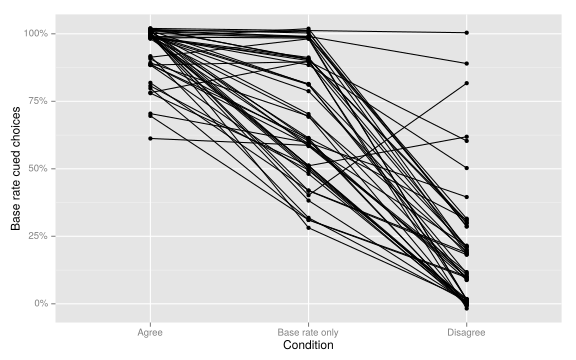
\includegraphics[width=.6\textwidth]{imgs/exp5_br_acc.pdf}
  \caption[Individual differences in the effect of descriptions
  on participants' responses, Experiment 5.]{
    Number of base rate responses per condition, by participant, in Experiment 5.
    \label{fig:exp5_br_acc} }
\end{figure}

\subsubsection{Effect of base rates on description choices}


Base rates had a significant main effect on
the number of description-cued responses given
($\chi^2$  = 67.7, DF = 2, p < .0001).
Pairwise comparisons showed that participants were
less likely to give the description-cued response
when the base rate disagreed with the description (80.4\%)
than when it agreed (94.4\%;
$e^{\beta}$ = 0.20, CI = [0.12, 0.36], z = 6.655, p < .0001)
or when the base rate was uninformative (93.6\%;
$e^{\beta}$ = 0.24, CI = [0.14, 0.42], z = 6.128, p < .0001).
There was no difference between trials in which the base rate agreed
and those where the base rate was uninformative (z < .3, p > .7),
with both conditions close to ceiling.
Therefore, participants were at least in some way
sensitive to the base rate information, and in a minority of cases
relied on it instead of the description when the two conflicted.

Once again, it is useful to investigate individual differences in this effect.
The left panel of Figure~\ref{fig:exp5_description_acc} shows
the proportion of description-cued responses given by each participant by condition.
This shows three participants who were substantially less likely
to give the description-cued response when the base rate disagreed with it.
The right panel shows the difference, for each participant,
in the number of description-cued responses given
from when the base rate agreed to when it disagreed.
This shows that, along with the 
three participants who showed a substantial change,
most participants showed a moderate effect in the same direction:
they were slightly less likely to select
the description-cued response when the base rate disagreed with it,
suggesting that base rates had some effect on the majority of participants.
Out of 50 participants, 28 were less likely
to select the description-cued response when the base rate disagreed,
13 were equally likely to do so (including 10 who always gave this response),
and 9 were actually more likely to select the description-cued response
when the description disagreed.

\begin{figure}[ht]
  \centering
  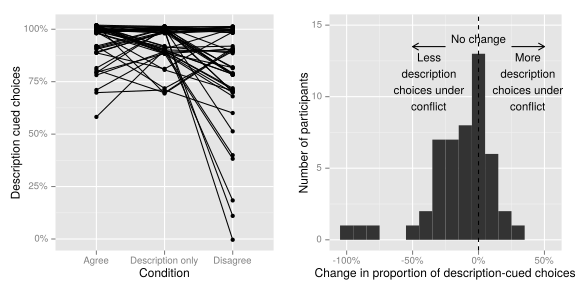
\includegraphics[width=\figurewidth]{imgs/exp5_description_acc.pdf}
  \caption[Individual differences in the effect of base rates
  on participants' responses, Experiment 5.]{
    \label{fig:exp5_description_acc}
    Left: Proportion of base rate-cued responses given in each condition,
    by participant.
    Right: Difference in the proportion of description-cued responses given
    by each participant between when the base rate agreed and disagreed with
    the description. Values below 0 indicate a participant was less likely
    to select the description-cued response when it conflicted with the base rate
    than when it agreed.
  }
\end{figure}



\subsection{Descriptive statistics}

Next, I calculated a number of descriptive statistics for each trial.
Maximum deviation of mouse cursor trajectories was bimodally distributed
(see Chapter 2; Bimodality Coefficient = .567; Hartigan's D = .0224, N = 1499, p < .0001)
and so trajectories were classified as either direct or reversals,
as described in Appendix~\ref{appendix:reversals} (reversal cut-off: MD > 0.972).

When the cues conflicted,
participants who gave the base rate-cued response
spent more time reading the description (3,229 msec, SD = 2,943)
than those who gave the description-cued response
(2,406 msec, SD = 2.789;
$e^{\beta}$ = 125\%, CI = [104\%, 150\%],
t(484.0) = 2.368, p = .018),
and were slower to initiate their mouse movements
(456 msec, SD = 266 vs. 476 msec, SD = 326;
$e^{\beta}$ = 119\%, CI = [110\%, 129\%],
t(486.8) = 4.496, p < .0001),
but did not differ in their response times (p > .5).
Participants were also more likely to
initially move towards the description-cued option
before selecting the base rate-cued one
(38\% of base rate responses)
than to initially move towards the base rate-cued option
and ultimately select the description-cued one
(27\% of description-cued responses;
$e^{\beta}$ = 1.7, CI = [1.03, 2.9],
z = 2.109, p = .035).

\subsubsection{Effect of descriptions on base rate choices}

Table~\ref{tbl:exp5_br_descriptives} shows these descriptive statistics
for trials where the  base rate response was given,
broken down for each type of description.
Table~\ref{tab:exp5_br_betas} shows effect sizes for
the main effect of description type, and pairwise comparisons between descriptions,
for each variable shown in Table~\ref{tbl:exp5_br_descriptives}.

\begin{table}[h]
  \centering
  \caption[Descriptive statistics for base rate-cued responses, Experiment 5.]{
    Descriptive statistics for trials where the base rate-cued response was given in Experiment 5.
    All times are in msec. Standard deviations are shown in parentheses.
    Trials are broken down according to whether the description
    agreed with the base rate, was uninformative,
    or disagreed with the base rate. \\
    \emph{Note:} N = Number of trials in which this response was given.
    \label{tbl:exp5_br_descriptives}
}
  %% \begin{tabular}{lrrrrrrr}
  \begin{tabular}{p{3cm} p{2.5cm} p{2.1cm} p{2.1cm} p{1.75cm} p{1.75cm} }
    \toprule
    %% Condition                  &  \shortstack{Reading time}  & \shortstack{Reading\\time}
    %% & \shortstack{Reading\\time} & Reversals & N   \\
    Description   &  Reading time  & Initiation time & Response time & Reversals & N   \\
    \midrule
    Agreed        &  2,186 (2,153) & 444 (247)       & 1,372 (522)   & 26\%      & 472 \\
    Uninformative &  3,046 (2,890) & 451 (241)       & 1,509 (666)   & 31\%      & 347 \\
    Disagreed     &  3,229 (2,943) & 476 (326)       & 1,776 (739)   & 35\%      & 98  \\
    \bottomrule
  \end{tabular}
\end{table}



There was a significant main effect of
descriptions on reading times
($\chi^2$ = 21.7, N = 2, p < .0001).
When giving the base rate-cued response,
participants were significantly faster to read the description
when it agreed with the base rate (2,186 msec, SD = 2,153)
than when it was uninformative (3,046 msec, SD = 2,890;
$e^{\beta}$ = 76.1\%, CI = [60.9\%, 95.2\%],
t(33.4) = 2.841, p = .0202),
or when it disagreed with it (3,229 msec, SD = 2,943;
$e^{\beta}$ = 70.8\%, CI = [60.1\%, 83.5\%],
t(878.3) = 4.111, p < .0001).
Reading times did not differ between uninformative descriptions
and those that disagreed with the base rate (t < .7, p > .8).

\begin{table}[h]
  \centering
  \caption[Effects of manipulating description on base rate-cued responses, Experiment 5.]{
    Main effects and pairwise comparisons between conditions
    for the effect of condition on the descriptive statistics
    shown in Table~\ref{tbl:exp5_br_descriptives},
    from trials where the base rate-cued response was given.
    For the main effect, the $\chi^2$ statistic is shown,
    which was subjected to a chi-squared test with 2 degrees of freedom in each case.
    For pairwise comparisons, the exponentiated regression weights $e^{\beta}$ are shown,
    reflecting the percentage change in the variables that were log transformed
    (reading, initiation, and response times),
    and the odds ratio change for the binary outcome (reversals).
    \label{tab:exp5_br_betas}
  }
  \begin{tabular}{l L{1.8cm} L{1.8cm} L{1.8cm} l}
    \toprule
    Comparison              & Reading time    & Initiation time & Response time   & Reversals\\
    \midrule
    Main effect ($\chi^2$)  & 21.68 $^{****}$ & 0.42            & 34.93 $^{****}$ & 4.78 $^{.}$\\
    \midrule
    Agreed/Uninformative    & 76\% $^{*}$     &  98\%           & 93\% $^{***}$   & 0.7\\
    Agreed/Disagreed        & 70\% $^{***}$   &  97\%           & 82\% $^{***}$   & 0.7\\
    Uninformative/Disagreed & 93\%            & 99\%            & 89\% $^{**}$    & 0.95\\
    \bottomrule
    \multicolumn{5}{l}{ \emph{Note}: $^{.}$ p < .1; $^{*} p < .05;\ ^{**} p < .01;\ ^{***} p < .001;\ ^{****} p < .0001$ }
  \end{tabular}
\end{table}


Initiation times did not differ according to description type
($\chi^2$ < .5, N = 2, p > .8).
However, there was a main effect of description on response times 
($\chi^2$ = 34.9, N = 2, p < .0001).
Participants were faster to give the base rate-cued response
when the description agreed with the base rate (1,372 msec, SD = 522)
than either when the description was uninformative (1,509 msec, SD = 666)
%% t(29.3) = 3.631, p = .0030),
or when description disagreed with the base rate (1,776 msec, SD = 739).
%% t(980.5) = 5.520, p < .0001)
They were also faster when the description was uninformative
than when it disagreed with the base rate.
%% (t(177.8) = 3.231 , p = 0042).
All comparisons were statistically significant
(t's > 3.2, p's < .01).

There was a marginally significant effect of descriptions on reversals
---  the probability of initially moving towards
the alternative option before giving the base rate response
($\chi^2$ = 4.8, N = 2, p = .0916).
Despite this, none of the post-hoc comparisons approached significance.
However, the trends were in the direction predicted by dual process accounts.
On trials where participants gave the base rate-cued response,
a greater proportion changed their mind while doing so
when the description cued the opposite response
than when the description was uninformative,
and fewer again did so when the description agreed with the base rate.

In summary, consistent with what would be predicted by most dual process accounts,
participants were indeed slower to give the base rate-cued response
when it went against the contents of the description,
and spent longer reading the description for such problems.
For trials where the base rate-cued response was given,
descriptions did not have a significant effect
on participants' initial cursor movements, in contrast to previous experiments.
This pattern, however, can be better understood
by considering the transition probability analyses, below.


\subsubsection{Effect of base rates on description choices}

Table~\ref{tab:exp5_d.descriptives} shows descriptive statistics
for trials in which the description-cued response was given, by condition.
Contrary to a number of previous studies that found evidence that
base rates interfere with participants' description-cued responses,
there was no main effect of condition found on any of the descriptive measures here
($\chi^2$  < 3.4, DF = 2, p > .18).
Focusing on response time, the measure most commonly analysed in previous studies,
reveals a weak trend in the expected direction.
Response times when both cues agreed (1,372 msec, SD = 522)
were almost identical to when only the description was informative (1,369 msec, SD = 464),
but slightly faster than when the base rate cued the opposite response (1,402 msec, SD = 563).

\begin{table}[h]
  \centering
  \caption[Descriptive statistics for description-cued responses, Experiment 5.]{
    Descriptive statistics for trials where the description-cued response
    was given in Experiment 5.
    Trials are broken according to whether the base rate
    agreed with the description, was uninformative,
    or disagreed with the description.\\
    \emph{Note:} N = Number of trials in which this response was given.
    \label{tab:exp5_d.descriptives}
  }
  %% \begin{tabular}{lrrrrrr}
  \begin{tabular}{p{3cm} p{2.5cm} p{2.1cm} p{2.1cm} p{1.75cm} p{1.75cm} }
    %% Condition        & \shortstack{Description\\Responses} & 
    %%                    \shortstack{Reading\\time} &
    %%                    \shortstack{Initiation\\time} & 
    %%                    \shortstack{Response\\time}  &
    %%                    Reversals & N  \\
    %% Condition        & Reading time  & Initiation time & Response time & Reversals & N  \\
    %% Condition                  &  \shortstack{Reading time}  & \shortstack{Reading\\time}
    %% & \shortstack{Reading\\time} & Reversals & N   \\
    \toprule
    Base rate     &  Reading time & Initiation time & Response time & Reversals & N   \\
    \midrule
    Agreed        & 2,186 (2,153) & 444 (247)       & 1,372 (522)   & 29\%      & 472\\
    Uninformative & 2,309 (2,260) & 447 (258)       & 1,369 (464)   & 28\%      & 467\\
    Disagreed     & 2,406 (2,789) & 456 (266)       & 1,402 (563)   & 27\%      & 401\\
    \bottomrule
  \end{tabular}
\end{table}


In previous tests of the intuitive logic theory
\citep[e.g.][see also \citealp{Pennycook2015}]{DeNeys2011b,Mevel2014},
researchers have explored the relationship between
individual differences in overt sensitivity to normative principles
(i.e. the proportion of normatively correct responses given on conflict trials)
and implicit measures of  conflict.
Therefore, I calculated, for each participant,
the proportion of description-cued responses on conflict trials.
Of the 50 participants, 26 gave the description-cued response
on 9 or 10 of the 10 conflict trials,
and were classed as \emph{description-driven reasoners}.
The remaining 24 participants gave
the description-cued response on average 62\% of the time,
and were classed as \emph{equivocal reasoners}.
Only 4 of these participants gave the base rate-cued response
on more than half of the conflict trials.

I repeated the analyses described above ---
analysing reading time, movement initiation time, response time, and proportion of reversals,
on trials where the base rate-cued response was given ---
using 3 (description: agreed, uninformative, or disagreed with base rate)
by 2 (type of reasoner: description-driven or equivocal) factorial mixed models,
with random intercepts for each participant and each problem.
None of these models showed significant description by type of reasoner interactions (p's > .1),
indicating that there were no substantial individual differences in
the null effects of manipulating the description reported above.


However, the analyses reported here are in some ways conservative.
Working within the null hypothesis significance testing (NHST) framework,
I have calculated p values, comparing the main effect of base rate types
on participants' response times to what would be expected under the null hypothesis.
Because there were three kinds of base rate ---
they could agree with the descriptions, be uninformative, or disagree ---
I then performed pairwise comparisons,
using the Tukey HSD method to adjust the p values
to maintain a Type 1 error rate of 5\%.
While I was unable to reject the null hypothesis
--- that base rates did not influence participants
on trials where they gave the description-cued response ---
this framework does not make it possible to accept this null hypothesis either.

Therefore, I conducted a follow up analysis,
comparing responses where the base rate agreed with the description
to those where it disagreed,
and used Bayesian inference to estimate
the magnitude of the difference in response time between these two conditions.
Participants on average responded in 1,372 msec (SD 522 msec) when the cues agreed,
and 1,402 msec (SD 563 msec) when they disagreed, a slowdown of 30 msec, or 2.1\%.

I fit a Bayesian multilevel model using Stan 
\citep{StanDevelopmentTeam2015},
where log-transformed response times for
description-cued responses when the base rate agreed with the description
where compared to those where the base rate disagreed.
The model included random intercepts
for each participant, and for each problem.
Uninformative priors were set on all model parameters.
The full model specification can be found in Appendix~\ref{appendix:exp5_bayes}.

After sampling,%
\footnote{
  I ran 8 MCMC chains of 1000 iterations each,
  with 500 warm-up draws discarded from each chain.
  }
the posterior distribution for the intercept term
(the mean response time when the base rate agreed),
had a median estimate of 1,357 msec
and a 95\% credible interval%
\footnote{
  A Bayesian 95\% credible interval can be interpreted in the way
  that frequentist confidence intervals are often misinterpreted:
  we can be 95\% sure that the true value
  lies between these lower and upper bounds,
  given our prior beliefs and the current data.}
of [1,285 msec; 1,423 msec].
More importantly, posterior on the regression weight $e^{\Beta}$
is shown in Figure~\ref{fig:exp5_posterior}.
The median estimate was 102.8\%, indicating a 2.8\% slowdown under conflict,
and the 95\% credible interval was [99.0\%; 106.7\%].
Therefore, while the most credible effect is a very small slowdown under conflict,
there is considerable uncertainty around this effect.
We can further understand this estimate by looking to
the mass of the posterior above and below certain values.
For instance, we can be 91.9\% certain
that response times under conflict were \emph{slower} than those when the cues agreed
--- that is, $e^{\beta}$ > 100\% ---
but also 99.1\% certain that the slowdown did not exceed 10\%
of the response time when the cues agreed.
Another way of interpreting a posterior of this sort \citep{Kruschke2011}
is to define a range of effect sizes that we would consider to be trivial
--- that is, to define a \emph{region of practical equivalence}; ROPE.
For us to be 95\% confident that this effect constitutes a null result,
we would need to define all changes in response time
from 94\% to 106\% as being essentially null effects.
As I believe that effects within this range would be of theoretical importance,
the current results do not support the null hypothesis.



\begin{figure}[ht]
  \centering
  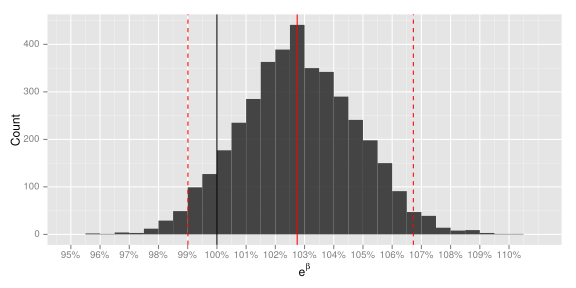
\includegraphics[width=.75\textwidth]{imgs/posterior.pdf}
  \caption[Bayesian analysis of effect of the base rate
    on rt for description-based responses, Experiment 5.]{
    \label{fig:exp5_posterior}
    Posterior samples for the $e^{\beta}$ regression weight,
    reflecting the difference in response times
    between description-based responses when the base rate agreed with the description
    and those when the base rate disagreed.
    The median estimate of 102.8\%
    (solid red line, dashed lines show 95\% credible intervals)
    indicates that participants were 2.8\% slower when the base rate disagreed.
    The solid black line shows the null effect.
  }
\end{figure}

In summary, the evidence here was not sufficient
to reject the null hypothesis in a NHST ANOVA design.
However, when I directly contrasted trials where
the base rate agreed with the description
to those where they disagreed,
the data supported an extremely small conflict effect with considerable uncertainty,
rather than the null hypothesis of no effect whatsoever.
Ultimately, the present data are inconclusive,
and fail to provide strong evidence
either of a slow-down under conflict,
or of the absence of such a slow-down.


\subsection{Cursor trajectories}


As described in Chapter 2,
cursor transition probabilities were calculated for each condition.
When base rates and descriptions disagreed,
participants initially moved towards
the option cued by the description on 66\% of trials,
selected this option after initially moving towards it 89\% of the time,
and selected the base rate-cued option after
initially moving towards it 36\% of the time.



\subsubsection{Effect of descriptions on base rate choices}




\begin{figure}[ht]
  \begin{floatrow}
    \ffigbox[.5\textwidth]{%
      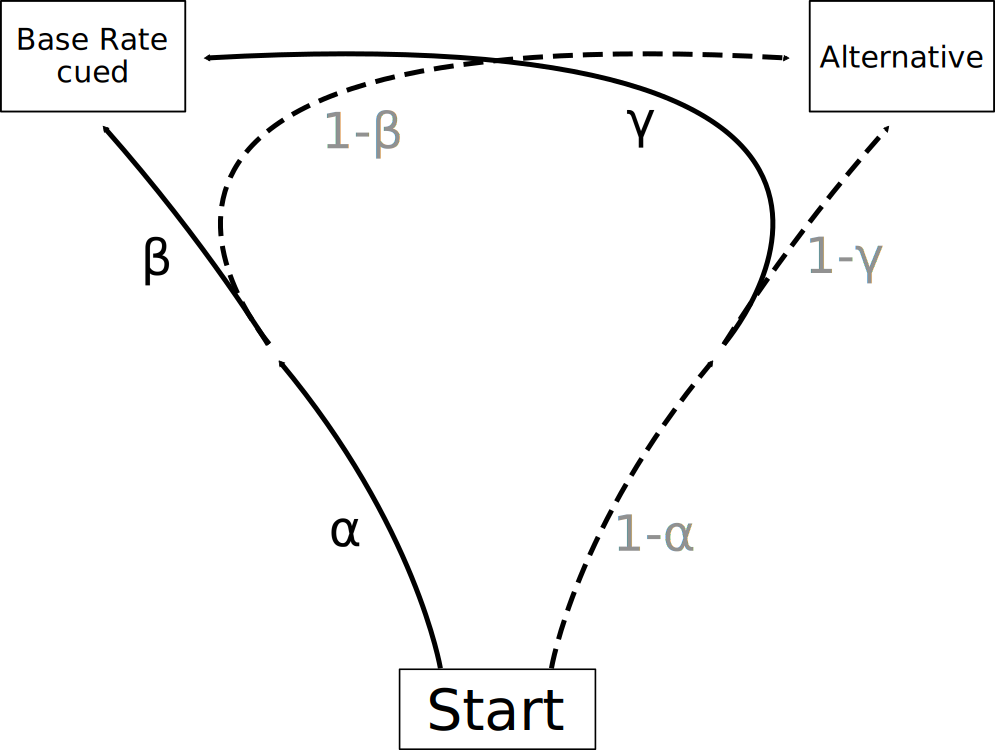
\includegraphics[width=.5\textwidth]{imgs/br_transitions.pdf}
    }{%
      \caption{
        The possible transitions that can occur during a trial
        where the base rate cues a response.
        \label{fig:exp5_br_transitions}
      }
    }
    \capbtabbox{%
      \centering
      \begin{tabular}{llll}
        \toprule
        Description   & $\alpha$ & $\beta$ & $\gamma$\\
        \midrule
        Agreed        & 69.4\%   & 96.5\%  & 89.5\%\\
        Uninformative & 57.4\%   & 79.1\%  & 56.3\%\\
        Disagreed     & 33.8\%   & 36.1\%  & 11.2\%\\
        \bottomrule
      \end{tabular}
    }{%
      \caption[Effect of descriptions on transition probabilities, Experiment 5.]{
        Transition probabilities for trials where the description either
        agreed with the base rate, was uninformative,
        or disagreed with the base rate.
        %% In this analysis $\alpha$ represents the proportion of trials
        %% that initially moved towards the base rate-cued option,
        %% $\beta$ the proportion that select that option
        %% after moving towards it,
        %% and $\gamma$ the proportion who selected the base rated-cued option
        %% after moving towards the alternative.
        There were significant main effects of description type,
        and significant pairwise differences between each description,
        on all measures.
        %% and significant pairwise differences
        %% between each description for all three proportions (p's < .001).
        \label{tab:exp5_br_transitions}
      }%
    }
  \end{floatrow}
\end{figure}



There was a significant main effect of the description type
on the proportion, $\alpha$ of trials where
initially moved towards the base rate-cued option
($\chi^2$ = 135.9, DF = 2, p < .0001).
Participants were most likely to initially move towards
this option
when the description also cued it (69.4\%),
less likely when the description was uninformative (57.4\%)
and least likely when the description cued the alternative option (33.9\%).
Pairwise comparisons between each description type
were all statistically significant
(z's > 3.9, p's < .001).

$\beta$ indicates the proportion of trials
where participants selected the base rate-cued option
after initially moving towards it.
There was a significant main effect of description type on this measure
($\chi^2$ = 262.7, DF = 2, p < .0001).
Participants were most likely to select the base rate-cued option
after initially moving towards it
when the description also cued that option (96.5\% of trials),
less likely when the description was uninformative (79.1\%)
and least likely when the description cued the alternative option (36.1\%).
Pairwise comparisons between each description type
were again all statistically significant
(z's > 5, p's < .0001).


Lastly, $\gamma$ reflects the proportion
of trials where participants selected the base rate-cued option
after initially moving towards the alternative option.
There was a significant main effect of description type
($\chi^2$ = 301.4, DF = 2, p < .0001).
Participants were most likely to change direction
and select the base rate-cued option
after initially moving towards the alternative
when the description agreed with the base rate (89.5\% of trials),
less likely when the description was uninformative (56.3\%),
and were very unlikely to change direction
when that alternative was cued by the description (11.2\%).
Pairwise comparisons between each description type
were once again all statistically significant
(z's > 5, p's < .0001).

These results show that description interfered with
participants' base rate-based reasoning at every juncture,
influencing both their initial mouse movements,
and their subsequent responses,
regardless of their initial movement.


\subsubsection{Effect of base rates on description choices}




\begin{figure}[ht]
  \begin{floatrow}
    \ffigbox[.5\textwidth]{%
      \includegraphics[width=.5\textwidth]{imgs/desc_transitions.pdf}
    }{%
      \caption{
        The possible transitions that can occur during a trial
        where the description cues a response.
        \label{fig:exp5_desc_transitions}
      }
    }
    \capbtabbox{%
      \centering
      \begin{tabular}{llll}
        \toprule
        Base rate     & $\alpha$ & $\beta$ & $\gamma$\\
        \midrule
        Agreed        & 69.4\%   & 96.5\%  & 89.5\%\\
        Uninformative & 68.5\%   & 98.0\%  & 84.1\%\\
        Disagreed     & 66.1\%   & 88.8\%  & 63.7\%\\
        \bottomrule
      \end{tabular}
    }{%
      \caption[Effect of base rates on transition probabilities, Experiment 5.]{
        Transition probabilities for trials where
        the base rate either agreed with the description,
        was uninformative, or disagreed with the description.
        %% In this analysis $\alpha$ represents the proportion of trials
        %% that initially moved towards the description-cued option,
        %% $\beta$ the proportion that select that option
        %% after moving towards it,
        %% and $\gamma$ the proportion who selected the description-cued option
        %% after moving towards the alternative.
        There was no effect of base rate type on $\alpha$.
        $\beta$ and $\gamma$ were both significantly lower
        (that is, participants were less likely to select
        the description-cued option, regardless of initial movement direction)
        when the base rate disagreed with the description.
        \label{tab:exp5_desc_transitions}
      }%
    }
  \end{floatrow}
\end{figure}



The transition probability analysis was repeated
to explore the effect of manipulating the base rate
on participants' movements towards the description-cued option.
Transition probabilities,
broken down according to the base rate,
are shown in Table~\ref{tab:exp5_desc_transitions}.
Here, $\alpha$ represents the proportion of trials
where participants initially moved towards the description-cued option.
There was no main effect of base rate on this proportion
($\chi^2$  = 1.5, DF = 2, p > .4):
participants initially moved towards the description-cued option
on average 68\% of the time,
regardless of the base rate information.

There were, however, main effects of base rate type
on $\beta$, the proportion of trials where
the description-cued option was selected after
participants initially moved towards it,
and $\gamma$, the proportion of trials where
the it  was selected after
participants initially moved towards the alternative option
($\chi^2$s  > 30, DF = 2, p's < .0001).
In both cases, participants were less likely
to ultimately select the description-cued option
when the base rate cued the other response option
than when the base rate was uninformative
or when it agreed with the description
(z's > 3, p's < .001; see Table~\ref{tab:exp5_desc_transitions}).

Therefore, base rates had no early impact on participants'
description-based reasoning,
and did not influence their initial mouse movements.
They showed some effect, however, on ultimate responses,
as participants were less likely to select the description-cued option,
regardless of what direction they initially moved the cursor.

\subsection{Time Course}

There are many time course analyses that
could be presented for this experiment,
and so for brevity, I report only the most informative comparisons here.
To explore the effect of varying the description
on participants' base rate-based reasoning,
I examined the proportion of trials on the side of the screen
containing the base rate-cued option,
on trials containing such an option.
Likewise, to explore the effect of varying the base rate
on description-based reasoning,
I examined the proportion of trials on the side of the screen
containing the description-cued option,
on trials such an option existed.
Both comparisons are plotted in Figure~\ref{fig:exp5_timecourse}.


\begin{figure}[ht]
  \centering
  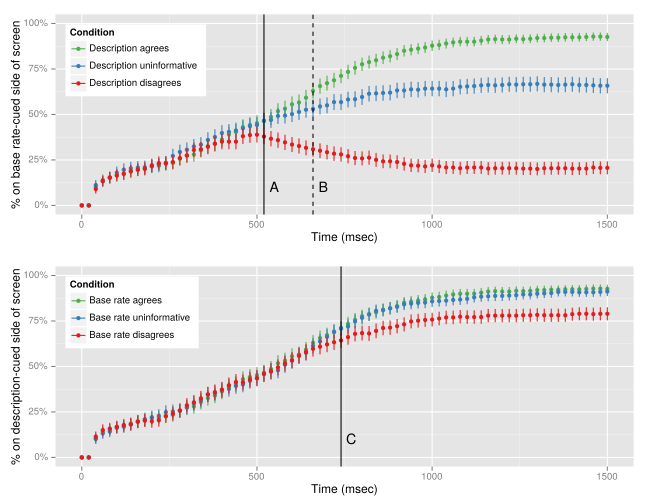
\includegraphics[width=\figurewidth]{imgs/exp5_timecourse.pdf}
  \caption[Time course plots for the effect of descriptions
    on base rate-cued choices, and vice versa, in Experiment 5.]{
    \label{fig:exp5_timecourse}
    Top: Proportion of trials where the cursor is
    on the side of the screen containing the base rate-cued option, over time,
    for trials where the description agreed with the description,
    is uninformative, or disagreed with it.
    Line A shows the onset of a significant difference between
    when the description disagreed with the base rate and the other two conditions.
    Line B shows the onset of a difference between when the description agreed
    and when it is uninformative.
    \\
    Bottom: Proportion on the side containing the description-cued option,
    for trials where the base rate agreed with the description,
    is uninformative, or disagreed with it.
    Line C shows the onset of a difference between
    when the base rate disagreed with the description and the other two conditions.
  }
\end{figure}

Divergence points were found as before,
by fitting two series of logistic mixed models.
The first predicted the proportion of trials on
the base rate-cued option's side of the screen,
with description type
(agreed with base rate, uninformative, or disagreed) as a predictor.
The second predicted the proportion of trials on
the description cued option's side of the screen,
with base rate type
(agreed with description, uninformative, or disagreed) as a predictor.
All models included random intercepts for each participant.
In each series, a model was fit to each 20 msec time window,
and divergence points for each pairwise comparison were defined as
the times after which these comparisons were found to be
statistically significant.
 
In both plots shown in Figure~\ref{fig:exp5_timecourse},
participants were equally likely to move towards each option
in any condition over the first 500 msec of each trial,
indicating that neither descriptions nor base rates
influenced participants' cursor movements before this time.

The effect of descriptions on base rate-driven reasoning was the first to manifest:
participants were significantly less likely
to place the cursor on the side of the base rate-cued option
when the description disagreed with the base rate
than when it agreed, or was uninformative,
from 520 msec onwards (line A in Figure~\ref{fig:exp5_timecourse}).
Later, they were more likely to move the cursor to this side of the screen
when the description agreed with the base rate
than when it was uninformative from 660 msec (line B in Figure~\ref{fig:exp5_timecourse}).

The effect of the base rates on description-driven reasoning was slowest to arise.
Participants became less likely to be
on the side of the screen containing the description-cued option
when the base rate disagreed with the description
than when it was agreed or was uninformative
from 740 msec onwards (line C in Figure~\ref{fig:exp5_timecourse}).
Mirroring the analysis of responses on these trials, above,
no difference emerged between
trials where the base rate agreed with the description
and trials where the base rate was uninformative.




\section{Discussion}

In this experiment, I combined mouse tracking with
a forced choice version of the base rate neglect task,
where I manipulated both the descriptions,
and the base rates participants reasoned about.
In doing so, I build on two lines of research.
Much earlier work in the heuristics and biases and dual process literature 
\citep[i.e.][]{Kahneman2011,Kahneman1973}
claims that descriptions are processed easily and automatically by Type 1 processes,
while processing base rate information
requires the optional later engagement
of more effortful Type 2 processes.
As a result, base rates are more likely to be ignored or underweighted.
More recent accounts \citep[i.e.][]{DeNeys2012,Barbey2007}
mostly agree with this fundamental dual process interpretation,
but argue that base rates play a more involved role in reasoning,
either because they can be processed by Type 1 processes 
\citep{DeNeys2012}, 
or because Type 1 and 2 processes operate in parallel
\citep{Sloman1996,Barbey2007}.


Analysis of problems in this experiment where
base rates and descriptions conflicted
provided support for a generic dual process account.
Participants gave the response cued by the description
on 80\% of such trials,
and when doing so were faster to read the description,
faster to respond,
and less likely to initially move the mouse cursor
towards the opposite option than on trials
where they gave the base rate-cued response.
Participants were also much more likely to
initially move the mouse cursor towards the description-cued option
than the base rate-cued option when the cues disagreed (doing so 66\% of the time),
and more likely to change direction if their initial movement
was towards the base rate-cued option.

Most dual processes accounts ---
the exception being a selective model \citep{Klaczynski2000,Chaiken1987}
where one or other kind of processing is engaged for a given task ---
would predict that participants who do give the response cued by the base rate
should be conflicted while doing so,
as they must inhibit the pull of the description-cued response.
This prediction was tested by analysing
all trials where participants could rely on the base rate,
and looking at effect of manipulating the description.

Consistent with this prediction,
the contents of a problem's description had a strong effect
on participants' base rate-cued reasoning,
as participants were most likely to give the base rate-cued response
when this response was also supported by the description (94\% of trials),
less likely when the description was uninformative (69\%),
and as mentioned above, only selected the base rate-cued response
when it conflicted with the description on 20\% of trials.

Similarly, when they did give this base rate-cued response,
participants both spent longer reading the description,
and spent longer responding,
when the description conflicted with the description than when it agreed.
This suggests that
participants had to inhibit the description-cued response
before they could give the base rate-cued response instead.
Unlike previous experiments in this thesis, however,
participants' were not significantly more likely to trace
reversal trajectories towards the base rate-cued option
under conflict, although the trend was in this direction.

The transition probability analysis (Table~\ref{tab:exp5_br_transitions})
similarly showed that descriptions had a pervasive effect
on participants' base rate-driven reasoning,
influencing both their initial movements,
and their ultimate responses regardless of initial movement direction.
The transition probabilities also allow us to
make sense of the non-significant effect of descriptions
on the probability of participants following a reversal trajectory
when giving the base rate-cued response.
Regardless of the base rate,
participants initially moved towards the description-cued option,
where available, on two thirds of trials.
Given that they were no more likely to initially
move towards the alternative option
when the base rate cued it than when it did not,
we must assume that base rates play no role at this point.
Later in reasoning, the influence of the description is even greater, 
dictating 80\% of final responses when it conflicts with the base rate,
and 94\% both when it agreed and when the base rate was uninformative.
At this point, base rates also clearly play a role,
as the response not cued by the description
is given on only 6\% of trials when it is not cued by the base rate either,
but 20\% when it is cued by the base rate.
To simplify, it appears that only the descriptions,
and random variations, have an effect on initial movements,
while later movements are even more influenced by descriptions,
and also slightly influenced by base rates.
The time course data are also in line with this interpretation,
as base rates had no influence on early movements.
When they did show an effect, after 740 msec,
this only slightly reduced the pull of the description-cued option
rather than reversing it,
as was the case in Experiments 1 and 2, for instance
(see the bottom panel of Figure~\ref{fig:exp5_timecourse}).





While these results are consistent with most
dual process accounts of this task,
some accounts, such as the intuitive logic theory \citep{DeNeys2012,Handley2015},
or a parallel-competitive dual process theory \citep{Barbey2007,Sloman1996},
further predict conflict in the opposite direction,
with participants who base their responses on descriptions
nevertheless showing sensitivity to the base rate information,
and experiencing conflict when base rates and descriptions disagree.

Analysis of participants' responses
on trials where the description cued a response showed
some evidence of sensitivity to base rates,
with participants less likely to give the description-cued response
when it conflicted with the base rate
than when the base rate agreed with the description, or was uninformative.
However, on such conflict trials participants
still overwhelmingly gave the response cued by the description.
Analysis of individual differences here
(Figure~\ref{fig:exp5_description_acc})
showed that the majority of participants' responses
appeared to be slightly influenced by the base rate,
with a small minority strongly influenced by it.

In contrast to previous tests of the intuitive logic theory, however,
\citep{DeNeys2008,DeNeys2008a,Franssens2009,Pennycook2012a}
there was no significant evidence that participants were
influenced by base rates on trials where their responses
were driven by the description,
as their reading times, movement initiation times,
response times, and cursor trajectories
did not differ significantly when the base rate
agreed with the description, was uninformative, or disagreed with it.
However, the trends were in the direction predicted by the intuitive logic account,
with participants slower to respond when the base rate conflicted with the description.
An exploratory Bayesian analysis suggested that
the most plausible effect size was a 2.8\% increase in response times under conflict,
although the data was largely inconclusive.
there was considerable uncertainty around this tiny effect.

Analyses of the transition probabilities
and the time course data told the same story.
Participants' initial mouse movements,
and the position of the cursor before 740 msec,
were not influenced by changes in the base rate
on trials where participants could rely on the description.
Instead, participants were slightly less likely
to select the description-cued response option,
or to be on its side of the screen from 740 msec onwards,
when the base rate cued the alternative response.
Taken together, these results suggest that
base rates either dictated participants' response to a problem,
or were almost totally ignored


To recapitulate, the results of this experiment
provide further support for a dual process interpretation
of base rate neglect \citep{Kahneman2002,Kahneman2005},
where, fast, effortless, automatic Type 1 processes
underlie description-based reasoning,
and slower, effortful Type 2 processes underlie
base rate-based reasoning.
Results consistent with this interpretation
were found in all of the analyses reported.
Participants predominantly gave the description-cued response
when the base rate also cued it and when the base rate was uninformative,
and only did so slightly less when the base rate conflicted with the base rate.
Even when giving base rate-cued responses,
participants were conflicted when the description disagreed with the base rate.
Analysis of the cursor trajectories and the time course data
showed that descriptions dictated both early movements (from half a second)
and participants' actual responses.

The data were less consistent, however, with some intuitive logic accounts
\citep[i.e.][]{DeNeys2012,DeNeys2014a,Handley2015}.
These would predict that
even when participants give the response cued by the description,
they should be sensitive to manipulations of the base rate,
and previous studies have found such effects
\citep[i.e.][]{DeNeys2008,Pennycook2012a,Pennycook2014}.
Here, I found no significant effects of manipulating the base rate
on participants' cursor movements or response times
when they gave the description-cued response.
An exploratory Bayesian analysis, however,
showed that participants were very slightly slower (around 30 msec)
on these trials when the base rate disagreed with the description.
Thus, it is not possible to draw strong conclusions
either for or against the intuitive logic account
from the current data.

The absence of a significant intuitive logic effect
on response times in particular was surprising,
as response times have been used as a measure of this conflict
in a number of previous studies \citep[i.e.][]{DeNeys2008,Pennycook2012a},
outlined in Table~\ref{tab:previous_baserate_studies}.
Although it is difficult to say with certainty
why this experiment differs from previous work,
I can identify a number of possibilities.

First, a number of changes were made to 
the procedure used by \citet{DeNeys2008a}
in order for it to be compatible with the mouse tracking paradigm.
As discussed above, the way in which information
was presented here meant that participants were able to
process each trials' information at two points:
before clicking on the ``NEXT'' button to reveal the question (reading time),
and after seeing the question but before responding (response time).
However, even when I combined these times (not reported),
there was little evidence of participants being slower
to give the description-cued response when it conflicted with the base rate.

The mouse tracking paradigm also requires that
participants respond under time pressure,
in this case within 6 seconds.
A visual timer in the centre of the screen
was used in this experiment to reinforce this idea,
filling up over the course of the allowed time.
As this time limit was only exceeded on 2 trials out of 2,000,
and average response times were below 2 seconds in all conditions,
I can be quite confident that participants did reason quickly,
although again this does not include
time spent reading the description.

These response are considerably faster than
those reported in the majority of previous conflict detection studies
that used the base rate paradigm
and measured response latencies, outlined in Table~\ref{tab:previous_baserate_studies}.
Moreover, of these studies, only two required participants to respond before a deadline.
\citet{DeNeys2008} presented participants in an fMRI scanner
with problems almost identical to those used here,
and required them to respond within 8.5 seconds of seeing the questions.
They found that participants were slower to give description-cued responses
when the cues conflicted (3.5 seconds) than any other condition ($\sim$2.8 seconds).
However, it should be noted that these response times were 
almost a second longer than those reported here,
at a time scale where this constitutes a $\sim$66\% increase.
Their result, while moderate in size ($\eta^2_p = .28$),
was also not robustly statistically significant,
with $F(1, 12) = 4.6, p_{rep} = .87$
(corresponding to approximately $p = .05$).

The other study reporting conflict effects at such a short time scale
was Experiment 2 of \citet{Pennycook2014},
where participants were asked to respond within 5 seconds.
Note, however, that this was an unusual base rate experiment.
Participants were instructed before each trial
to base their response on either ``belief'', or ``statistics'',
and in Experiment 2 asked to respond within 5 seconds.
Analysis of response latencies revealed conflict effects in both directions ---
when reasoning based on statistics, participants were slower 
if the description cued the opposite response,
and likewise slower when reasoning based on belief
if the base rate cued the opposite response.
However, these times remain a second or more slower
than those reported in the current experiment.
Furthermore, the magnitude of this effect was extremely small ---
going from 3.70 to 3.79 for statistics-based decisions ---
a small effect size ($\eta^2_p$) of .08.
It should also be noted that in Experiment 2 of \citet{Pennycook2014},
instructions to rely on belief or statistics were manipulated within-participants,
and so the effect within this short time window
could be in part due to task-switching effects \citep{Monsell2003}.
Experiment 3 of the same paper demonstrated
a similar effect with a between-participants manipulation,
but participants were not asked to respond quickly,
and the dependent variables were participants'
probability judgements and confidence ratings,
not their response times.
Therefore, it seems possible that in the current experiment
a) participants responded too quickly in most cases to detect 
the conflict between their responses and the base rate;
b) having not been explicitly told to use the base rate on 50\% of trials,
participants may have been less sensitive to the base rate
than those in  \citet{Pennycook2014}.

% \input{previous_baserate_studies_table}

\begin{table}
  \centering
  \caption[Prevous base rate neglect studies.]{
    Number of base rate-cued responses under conflict,
    and response latencies for description-cued responses
    when cues either agreed or conflicted,
    in previous base rate studies.}
  \label{tab:previous_baserate_studies}
  \rotatebox{90}{
    %% \begin{tabular}{ L{4cm} L{4cm} L{2cm} L{2cm} L{2cm}}
    \begin{tabular}{ p{.4\textwidth} p{.4\textwidth} p{.2\textwidth} p{.15\textwidth} p{.15\textwidth}}
      %% \begin{tabular}{\textwidth}{p{5cm}p{4cm}LLL}
      \toprule
      Study                                                                               &  Procedure                                          &  BR responses                &  No-conflict RT &  Conflict RT   \\[.75cm]
      \midrule                                         
      \citet{DeNeys2008a}                                                                 &  fMRI                                               &  45\%                        &  2.8            &  3.75          \\[.75cm]
      \citet{DeNeys2008}                                                                  &  Standard                                           &  22\%                        &  $\sim$14       &  $\sim$18      \\[.75cm]
      \citet{Franssens2009}                                                               &  Secondary load                                     &  47\%~(no~load) 35\%~(load ) &  $\sim$14       &  $\sim$17      \\[.75cm]
      \citeauthor{DeNeys2009a} (\citeyear{DeNeys2009a};~Exps.~2--4)                       &  Standard                                           &  $\sim$33\%                  &  $\sim$14       &  $\sim$17      \\[.75cm]
      %% \citet{DeNeys2011b}                                                              &  Confidence ratings                                 &  20\%                        &  NA             &  NA            \\[.75cm]
      \citeauthor{Pennycook2012a} (\citeyear{Pennycook2012a};~Exp.~4; extreme~base~rates) &  Standard                                           &  24--26\%                    &  16             &  20            \\[.75cm]
      \citeauthor{Pennycook2012b} (\citeyear{Pennycook2012b};~Initial responses)          &  Two-response paradigm \mbox{(probability~ratings)} &  N/A                         &  12.8           &  13.4          \\[.75cm]
      \citeauthor{Pennycook2014} (\citeyear{Pennycook2014};~Exp.~1)                       &  Belief/statistics instructions                     &  N/A                         &  $\sim$13       &  $\sim$14      \\[.75cm]
      \citeauthor{Pennycook2014} (\citeyear{Pennycook2014};~Exp.~2)                       &  Belief/statistics instructions, 5~second~deadline  &  N/A                         &  $\sim$3.8      &  $\sim$3.7     \\[.75cm]
      \bottomrule
    \end{tabular}
  }
  %% \end{tabulary}
\end{table}


Another factor may be the scarcity of base rate-cued responses
in general in the current experiment.
Reasonably, one would expect conflict detection to be 
related to participants' responses:
experiments that yield many base rate-cued responses
should also yield greater detection of conflict
on problems in which the description-cued response is given.
In this experiment, on the other hand,
the base rate-cued response was given on only 20\% of conflict problems,
perhaps unsurprisingly given the fast response times here,
and the robust finding that base rate responses
are slower than description responses.
Consequently, it may not be so surprising that
an experiment which yielded relatively few base rate-cued responses
should also show little influence of base rates 
on more subtle measures such as response time.

Lastly, recent work 
\citep[e.g.][]{DeNeys2010,Mevel2014} has highlighted
that there are individual differences in
this conflict detection process ---
not all participants are slower, or less confident,
when their responses conflict with base rates,
or with logical principles.
At present, we know relatively little about the factors
that make some participants, but not others,
sensitive to these conflicts.
Therefore, given that almost all studies in this area
reveal some participants for whom
the conflict detection effects do not hold,
it should perhaps not be surprising that 
these effects are not found in every study.

\subsubsection{Conclusions}

To conclude, this chapter reports one of the first uses of
the mouse tracking paradigm to investigate the interaction of
dual processes during reasoning.
Results are consistent with a default-interventionist
dual process accounts \citep{Evans2006,Kahneman2002,Evans2013a},
by which descriptions are processed easily and automatically
by Type 1 processes,
but base rates, thought to require Type 2 processes to process.
play less of a role in reasoning on most trials.
In fact, when the base rates were attended to,
they tended to dictate participants' responses outright.
The rich, temporal dynamics of the data collected
using this paradigm reveal much more about the underlying processes,
for instance that only descriptions influence
the initial direction of participants' cursor movements,
and that the descriptions have a discernible effect on cursor movements
from around 500 msec, while the weaker effect of base rates
is not apparent until around 750 msec.

A number of recent studies have also shown evidence
of conflict in the opposite direction,
as base rates have some effect on participants
even when their responses appear to be dictated by descriptions alone.
The current data, however, did not support this idea,
although this may in part be due to the ways in which
the experimental paradigm had to be adapted
to suit the mouse tracking paradigm,
in particular, the extremely faster response times,
and unusual presentation of information.
Despite this, however, the current chapter demonstrates 
another point at which conflict can be found in reasoning,
when the right kind of data is collected.

% % % % % % % % % % % % % % % % %
% % % % % % % % % % % % % % % % %
% % % % % % % % % % % % % % % % %
% % % % % % % % % % % % % % % % %











\chapter{Intuition vs. Reflection in Reasoning}
\graphicspath{{6.CRT/}}
%%% Local Variables: ***

\section{Introduction}

In Experiment 5 (Chapter 5), I used the mouse tracking paradigm
to study the interaction of two kinds of processes in cognition:
fast, intuitive \emph{Type 1 processes},
and slower, deliberative \emph{Type 2 processes}.
In that experiment, participants were asked to respond
within 5 seconds of seeing the probe question,
and my analyses focused on the responses they gave,
their response latencies,
and whether they moved the mouse straight to their response option
or went the wrong way initially.
However, reasoning is one of the most complex,
high-level cognitive processes possible,
and naturally not all reasoning happens in less than 5 seconds.
In this chapter, I use a slightly different
kind of mouse tracking paradigm
to investigate conflict in reasoning over a considerably longer time scale.
I do this for a task
that has become perhaps the classic means of pitting
intuition against logic: the Cognitive Reflection Test \citep{Frederick2005}.
Like Chapter 5,
this chapter addresses the question of
just how Type 1 and Type 2 processes
interact in dual process accounts of cognition.

\subsection{Cognitive Reflection and Reasoning}

The Cognitive Reflection Test \citep[CRT;][]{Frederick2005}
is a brief test designed to measure
individuals’ ability to inhibit intuitive responses
in favour of reflective and deliberative reasoning.
In the bat-and-ball problem, one of the best-know CRT items,
participants are asked:

\begin{quote}
  ``A bat and a ball together cost £1.10.\\
    A bat costs £1 more than a ball.\\
    How much does a ball cost?''
\end{quote}



The appealing but incorrect response, to say “10p”,
is believed to be generated effortlessly and automatically.
Arriving at the correct response of “5p” may require that
this intuitive response is inhibited in favour of
the result of sustained, effortful deliberation.

The CRT has become a widely-used measure of individual differences in cognition.
Higher CRT scores predict better performance on various cognitive tasks,
including reduced framing effects,
less discounting of delayed rewards
\citep{Cokely2009,Frederick2005}
and probability matching \citep{Koehler2009},
resistance to the illusion of explanatory depth \citep{Fernbach2013}
and conjunction fallacies \citep{Oechssler2009},
greater metacognitive awareness \citep{Mata2013a},
and less endorsement of supernatural beliefs
\citep{Pennycook2012,Shenhav2012},
less endorsement of vacuous statements as profound \citep{Pennycook2015b},
as well as performance on various tasks that pit normative responding against intuition
\citep{Toplak2011}
Scores on the CRT correlate with measures of IQ and personality characteristics,
and usually predict performance even when these are controlled for
\citep{Toplak2011}.


\subsection{Dual Process Accounts}

The CRT is widely seen as a an archetypal application of
dual process theories of cognition \citep{Frederick2005,Kahneman2005,DeNeys2013a}.
Consistent with this, performance on the CRT is related to
performance on a number of other traditional dual process tasks \citep{Toplak2011},
and to dispositional factors related to willingness to engage in analytic thinking
\citep{Campitelli2010a,Campitelli2013,Bockenholt2012}.

However, dual process theories differ in their account of CRT performance.
As discussed in Chapter 1, there are a number of ways in which
Type 1 and Type 2 processes can interact during reasoning.
As has been my focus throughout this thesis,
I will concentrate on the predictions made by each account
with regard to when conflict occurs during reasoning.
Although I am interested in reasoning in general,
I discuss these accounts in terms of
the specific points at which they predict
conflict should occur during the CRT.
According to a selective dual process account \citep[e.g.][]{Klaczynski2004},
the CRT, like all such tasks, should not evoke any conflict.
Instead, participants should selectively draw on heuristic Type 1 processes,
which usually produce a response of ``10p'' on the bat-and-ball problem,
or draw on Type 2 processes to apply the simple mathematical rules
needed to reach a correct response of ``5p''.
On the other hand, Type 1 processes are always automatically activated
in default-interventionist models \citep{Evans2006,Kahneman2011,Kahneman2005}.
Therefore, such accounts would predict that
heuristic responses (``10p'') come to mind automatically for most participants,
and that giving the correct response requires that this heuristic response is inhibited,
and that Type 2 processes are engaged to derive the correct response.
Such a default-interventionist account is assumed, for instance,
in \citegap{Frederick2005}{'s} paper introducing the CRT,
and \citegap{Toplak2011}{'s} work outlining the relationship between
the task and other dual process problems.

A third option \citep{Sloman2014,Sloman1996}
is that both Type 1 and Type 2 processes are activated simultaneously,
and that they compete for control of behaviour.
In common with default-interventionist models,
these accounts predict that Type 1 intuitive responses
must be inhibited in order to reason correctly.
Uniquely though, parallel models would also predict Type 2 processes
should attempt to signal the correct response,
even when failing to overrule the output of Type 1 processes.

The intuitive logic model \citep{DeNeys2012,DeNeys2014a}
has also been applied to performance on the CRT \citep{DeNeys2013a}.
This model modifies the traditional default-interventionist model
to account for many findings which indicate that
when participants provide biased, heuristic responses,
they are often implicitly aware of some conflict between
their responses and the normative standard.
According to this model, Type 1 processes are sensitive to normative principles,
such as logical principles in syllogistic reasoning tasks,
or mathematical rules on the bat-and-ball problem.
As a result, they implicitly signal a conflict when
the incorrect heuristic response is given.
However, because the heuristic response is usually prepotent,
participants often fail to inhibit it,
even when they do detect that it conflicts with normative principles.
It is unclear at present, however, how this conflict is actually detected.
One possibility is that Type 1 processes simultaneously produce
both heuristic and correct responses,
and it is the conflict between these two partially active beliefs
which is detected directly.
In Chapter 1, it is this proposition that I refer to
as the intuitive logic theory.
Alternatively, the process may be more subtle,
with Type 1 processes not generating a fully-formed correct response,
but rather detecting, through some other means,
that the heuristic response is questionable.
I refer to this proposition in Chapter 1
as the dual process conflict monitoring theory.
Clearly, these two possibilities make different predictions
about conflict between competing response options during reasoning.
In the former case, the intuitive logic model would,
like a parallel-competitive account, predict that
because both responses are partially cued,
participants should be drawn towards giving the correct response,
even when they ultimately give the heuristic one.
In the latter case, if Type 1 processes can signal conflict
without actually generating the correct response,
participants may experience conflict and uncertainty,
but not be actually drawn towards the correct response when giving the heuristic one.
For the purposes of this experiment,
the same predictions are made by the slightly different
intuitive logic account offered by \citet{Handley2015}.
For simplicity, I will refer to \citegap{DeNeys2012}{'}
account throughout, with the understanding that the same points generally apply
to other intuitive logic accounts.

As discussed in previous chapters, evidence of
the implicit conflict detection predicted by the intuitive logic model
comes from a range of experimental paradigms
\citep[see also][for a review]{DeNeys2012}.
Typically, these studies compare conflict problems,
where the intuitive, heuristic response is incorrect,
to analogous no-conflict versions,
where both heuristics and normative principles cue the same response.
Type 1 processes cue both the heuristic response on conflict problems
and the correct response on no-conflict problems.
If participants detect the conflict between
normative principles and their heuristic responses,
they should show greater evidence of conflict on these problems,
compared to the no-conflict problems.
Such conflict has been measured using confidence ratings
\citep{DeNeys2011b},
response times \citep{DeNeys2008},
neuroimaging \citep{DeNeys2008a},
and galvanic skin response \citep{DeNeys2010},
among other measures.

Two studies, however, directly test the intuitive logic model against the CRT.
\citet{DeNeys2013a} showed that heuristic responses on conflict problems
were given with less confidence than correct responses on no-conflict versions of the same problems.
\citet{Gangemi2015} report similar effects,
asking participants to fill out a brief questionnaire
measuring their ``feeling of error'' after answering either
the original bat-and-ball problem or a no-conflict control version,
both when participants were asked to generate their responses,
and when asked to choose between the heuristic and correct responses.
These findings all suggest that participants are to some extent
aware of the inadequacy of their heuristic responses. 


In this chapter I use a novel version of the mouse tracking paradigm
to explore this topic.
Participants completed a computer-based multiple-choice version of the CRT,
including both conflict problems,
where the intuitively appealing heuristic response was incorrect,
and no-conflict versions of the same problems,
where the appealing response was the correct one.
There  were four response options for each problem,
located in each corner of the display.
While participants decided on their response,
their mouse cursor movements were recorded
as they moved the cursor around the screen.
Unlike in previous mouse tracking studies,
participants were not placed under time pressure,
and their mouse movements over the first 60 seconds of each trial were analysed.
Rather than moving the cursor directly from its starting point
to a response option and clicking on it,
participants typically moved the cursor
around the screen a number of times on each trial,
passing close to multiple response options.
As mentioned in Chapter 1,
mouse movements over such long time scales
have been used in the past
as part of research on human-computer interaction,
typically involving users interacting with web pages,
such as web search results pages
\citep[e.g.][]{Chen2001,Rodden2008,Huang2011}
This allowed me to use the patterns in these cursor movements
to test predictions derived from the various forms of dual process theory.

According to a selective dual process account,
participants should move to the response option they eventually chose
without showing any particular attraction towards
any of the other options along the way.
According to a traditional default-interventionist account,
on conflict trials participants should initially be drawn
towards the heuristic response option,
but in some cases inhibit this response and instead select the correct option.
A parallel-competitive account would likewise predict that participants
are drawn towards the heuristic option on trials where they
eventually give the correct response,
but would also predict the reverse ---
because Type 2 processes are activated in parallel with Type 1,
participants should be in some cases drawn towards
the correct option even on trials where they
end up giving the heuristic response.
The predictions of the intuitive logic model
depend on the nature of the conflict detection process.
If participants detect conflict because
both responses are simultaneously generated by Type 1 processes,
then the intuitive logic model, like the parallel-competitive model,
would predict conflict in both directions.
Alternatively, if the conflict detection process is more subtle
(c.f. the dual process conflict monitoring theory, Chapter 1)
then like the classic default-interventionist account
it would predict that participants should be drawn to the heuristic option
when selecting the correct one, but not the other way around.




\section{Method}

\subsection{Participants}

One hundred and thirty one students at Queen’s University Belfast
participated in exchange for course credit.

\subsection{Materials}

Eight problems were adapted from
\citegap{Primi2015}{'s} extended version of the CRT.
Each of these problems was modified to create a set of
eight corresponding non-conflict problems,
in which the intuitively appealing responses were also the correct ones
(see the Appendix~\ref{appendix:exp6_stimuli}).
Participants were randomly allocated to complete either
conflict versions of items 1, 3, 5, and 7
and no-conflict versions of the rest, or vice versa.
Each problem was presented in a 4-option multiple choice format.
For the conflict items, the possible responses were the correct option,
the incorrect heuristic option, and two incorrect foil options.
For the non-conflict items the correct intuitive option was presented
with three incorrect foils.

\subsection{Procedure}

The experiment was administered on personal computers,
programmed using PsychScript (see Chapter 2),
and run in the web browser.
Participants were instructed to respond in their own time to each CRT problem
by clicking on one of the four response options
presented in the four corners of the display
(Figure~\ref{fig:exp6-screenshot}).
Participants were not made aware of
the mouse tracking aspect of the experiment in advance. 

\begin{figure}[ht]
  \centering
  \includegraphics[width=\figurewidth]{imgs/exp6-screenshot.png}
  \caption[A screen shot from the CRT, Experiment 6.]{
    \label{fig:exp6-screenshot}
    A screen shot from the CRT.
  }
\end{figure}

Each problem was preceded by onscreen instructions to
click on a button marked ``Go'', presented in the centre of the monitor.
This was done to ensure the mouse cursor was located
in the same central position at the beginning of each trial.
The button was then replaced by the problem text
and the four response options appeared simultaneously in the corners
(Figure~\ref{fig:exp6-screenshot}).
The response options were randomly assigned to the four locations on each trial,
with the constraint that the correct and heuristic response options
were always adjacent for conflict problems.
The mouse cursor was no longer visible at the onset of each trial
to prevent it from obscuring the question text.
The cursor reappeared once it had been moved more than 5\% of the width of the display.
Mouse cursor location was recorded every 20 msec.


\section{Results}

\subsection{By-trial analyses}

After excluding data from 3 participants 
who did not complete the experiment within the 15 minutes allocated, 
and 7 trials with response times greater than 100 seconds (.6\% of the total), 
participants selected the correct option on 79.5\% of non-conflict problems.
On the conflict problems, the correct option was chosen 36\% of the time,
the heuristic option 58\%, and one of the foils 6\% of the time.

In the first stage of the analysis, 
I calculate a number of summary statistics for each trial, 
and compare these between problem types, and between responses. 
The measures were response time, 
the distance travelled by the mouse cursor
(scaled so that a straight line from the start point
 to the response corresponds to 1 unit),
the number of times the cursor was moved during a trial
(with movements defined as windows of 100 msec or more in motion, 
separated by 100 msec or more not moving), 
the closest proximity achieved between 
the cursor and the non-chosen option
(closest proximity to the heuristic response option 
on trials where the correct option was chosen, and vice versa). 
These measures were compared using linear mixed models, 
with crossed random intercepts for each participant, 
and each problem \citep{Baayen2008}.
Response latencies, and the distance travelled by the mouse cursor
were log-transformed to normalise their distributions, 
and a generalised mixed model with a Poisson link was used
to model the number of movements. 

Consistent with a dual process interpretation, 
whereby heuristic responses are generated by Type 1 processes,
and correct responses under conflict by Type 2 processes,
for conflict problems there was greater evidence of conflict
across all measures when participants gave the correct response (N = 181) 
than the heuristic one (N = 297).
The average time to respond was 27.3 seconds (SD = 16.3) for correct responses, 
and 21.0 seconds (SD = 13.4) for heuristic responses
($e^{\beta}$ = 114\%, CI = [102\%, 129\%],
t(470.8) = 2.349, p = .0192).
The mouse cursor travelled a greater distance 
before selecting a correct option (6.11 times the minimum needed distance, SD = 5.6) 
than an heuristic option (5.66 times, SD = 4.74;
$e^{\beta}$ = 116\%, CI = [102\%, 133\%],
t(298.4) = 2.267, p = .0241). 
There were also more cursor movements on
trials in which the correct response was given (5.4, SD = 4.8) 
than when the heuristic response was given (4.9, SD = 4.5; 
$e^{\beta}$ = 1.15, CI = [1.02, 1.29],
z = 2.337, p = .0195).
Finally, the minimum distance between 
the cursor and the heuristic option on trials in which the correct option was chosen 
was on average 49\% of the display width (SD = 24\%),
significantly less than the minimum distance between
the cursor and the correct option 
on trials in which the intuitive option was chosen (55.5\%, SD = 18\%,
$e^{\beta}$ = 0.92, CI = [0.89, 0.96],
t(72.1) = 4.119, p < .0001).

Most tests of the intuitive logic model compare
correct responses on no-conflict problems with
heuristic responses on conflict problems, 
on the basis that heuristic, Type 1 processes should cue both kinds of response, 
but the chosen response conflicts with normative principles on conflict problems only. 
Evidence for the intuitive logic model 
therefore comes from results which indicate 
greater conflict for heuristic responses to conflict problems (N = 404). 
However, there was no such reduction in conflict for no-conflict problems
on any of the applicable measures:
response time (23.1 seconds, SD = 15.3; t(14.3) = 0.222, p > .8),
distance travelled (5.6, SD = 5.0; t(15.0) = 0.359, p > .7) 
and number of movements per trial (5.2, SD = 4.6; z = 0.064, p > .95).

Following previous intuitive logic studies
\citep[e.g.][see also \citealp{Pennycook2015}]{DeNeys2011b,Mevel2014},
I also calculated the number of heuristic responses given
by each participant on conflict problems, 
and categorised each participant as either
``majority heuristic'' (3 or 4 heuristic responses out of four, 53 participants)
or ``minority heuristic'' (0 to 2 heuristic responses, 75 participants). 
I entered this measure as a participant-level predictor in the models, 
but found that it was not involved with any interactions in the analyses above
(t's < .9, p's > .4). 
I also repeated this analyses for the most (4 heuristic responses) 
and least (one heuristic response) biased reasoners only, 
again finding so significant interactions (t's < 1.1, p's > .25).
Therefore, these analyses revealed no evidence for logical intuitions
in either biased or unbiased participants.



\subsection{Time Course Analyses}

\begin{figure}[ht]
  \centering
  \includegraphics[width=\figurewidth]{imgs/exp6-typical-trajectory.png}
  \caption[A typical cursor trajectory from Experiment 6.]{
    \label{fig:exp6-typical-trajectory}
    A typical mouse cursor trajectory from the conflict condition. 
    Numerical values indicate the time elapsed in seconds. 
    Cursors meandered as participants generated their responses, 
    passing near the response options located in the corners of the display
  }
\end{figure}

In most previous mouse tracking research,
both in this thesis and in general
\citep[e.g.][]{Freeman2011d,Spivey2005},
the location of the cursor is recorded over a few seconds,
as participants move it from a starting position to 
a response option located in either top corner of the screen.
Almost invariably, this path follows either a single movement
(curved or otherwise) to a response,
or as has been more the case in this thesis,
a movement towards one response, that changes direction mid-flight.
In the current data, unfolding over up to 60 seconds, 
participants move and rest the cursor many times throughout a trial,
an average of 5.1 times, and a maximum of 30.
Thus, this data is in ways more similar to eye movement data.
A typical mouse cursor trajectory is shown in Figure~\ref{fig:exp6-typical-trajectory},
showing  a number of movements which pass near to several response options. 
In order to analyse participants' attraction to each response option over time,
the display was divided into quadrants
corresponding to each response option.
For the first 60 seconds of each trial, 
the mouse cursor positions at each 200 millisecond time slice
were coded according to which section of the screen they occupied, 
similar to fixation analyses of eye-tracking data.

Figure~\ref{fig:exp6-all} shows, for each response region, 
the proportion of trials in which the cursor is in that region, over time,
for both conflict and no-conflict problems. 
While the proportions at 60 seconds here 
largely reflect participants' ultimate responses, 
earlier proportions show how these preferences developed over time. 
Both correct responses to no-conflict problems and 
heuristic responses to conflict problems
were intuitively appealing, and participants 
began to move towards both options from before 5 seconds.
At approximately 10 seconds, participants also began to move towards
the correct response option on conflict problems,
and the accumulation of cursors in the region 
of the heuristic option under conflict slowed accordingly. 
The proportion of cursors in the region of these foil response options 
declined steadily in both conditions. 
Note that the proportions for the foil response options 
are averaged across the two foil options on conflict problems, 
and three options on no-conflict problems.

\begin{figure}[hp]
  \centering
  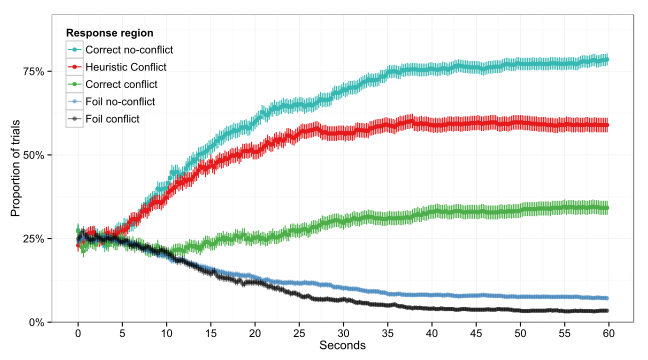
\includegraphics[width=\figurewidth]{imgs/exp6-all.pdf}
  \caption[Proportion of mouse cursors each region of the screen over time, Experiment 6.]{
    \label{fig:exp6-all}
    Proportion of mouse cursors in the region of the screen 
    corresponding to each response options, over time, 
    for conflict and no-conflict problems.    
  }
\end{figure}

\begin{figure}[bp]
  \centering
  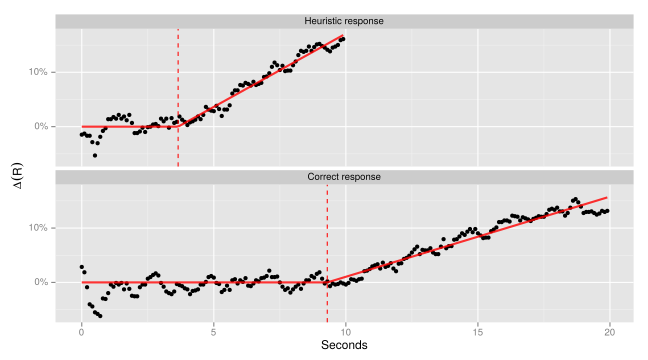
\includegraphics[width=\figurewidth]{imgs/exp6_changepoint.pdf}
  \caption[Change point analysis, Experiment 6.]{
    \label{fig:exp6_changepoint}
    Top: $\Delta (Heuristic)$, the difference between
    the probability of the cursor being in the region of the heuristic option
    and the probability of being in the region of a foil option.\\
    Bottom: $\Delta (Correct)$, the difference between
    the probability of being in the region of the correct option,
    and of being in the region of a foil option.
    Solid red lines show non-linear regression fits.
    Dashed vertical lines show change points,
    after which participants began to be drawn towards the option in question.
  }
\end{figure}

\subsubsection{Bayesian Change Point Analysis}

Inspecting Figure~\ref{fig:exp6-all},
participants are initially equally likely
to move toward each of the four response options
on conflict trials, doing so 25\% of the time.
This is the case until some time before 5 seconds,
at which point participants become more likely
to be in the region of the heuristic option
than the correct option, or either of the foils,
reflecting the point at which processes driving participants
towards the heuristic response exert their influence.
Similarly participants were equally likely to be
in the region of the correct option as the foils
until around 10 seconds,
and after this point more likely to be in the region of the correct option,
indicating that participants begin to be drawn towards the correct option
from this time.

Of course, visual inspection of these curves
is not a particularly accurate means of revealing
\emph{when} participants begin to be drawn towards each response option.
To formally estimate the times at which
participants began to move towards each response,
I calculated, across each 40 msec,
$\Delta (Heuristic)$: the difference between the average probability
of the cursor being in the region of the heuristic option
and the probability of being in the region of either foil option, as well as
$\Delta (Correct)$: the difference between the average probability
of being in the region of the correct option
and of being in the region of the foil option.
This yielded two series of values (Figure~\ref{fig:exp6_changepoint})
that were close to $0$ until participants
began to be drawn towards the response in question,
and increased over time after that point.

I modelled these series using a non-linear regression model
of the form

\begin{equation*}
  \Delta (R) =
  \begin{cases}%
    0          & \text{if}\ t\ <\ \tau_{R} \\
    \beta * (t-\tau_{R})  & \text{otherwise}%
  \end{cases}
\end{equation*}

where $t$ is the time in seconds,
$\tau_{R}$  is the point at which
participants begin to be drawn towards response $R$,
and $\beta$ is the slope of the regression line
after time $\tau_{R}$.

Modelling $\Delta (Heuristic)$, I analysed the first 10 seconds of each trial,
and set a uniform prior on the value of $\tau_{Heuristic}$ between 0 and 10 seconds
(i.e. that participants were equally likely to start being drawn
towards the heuristic response any time between 0 and 10 seconds into a trial).
Modelling $\Delta (Correct)$, I analysed the first 20 second,
and again set a uniform prior on $\tau_{Correct}$ between 0 and 20 seconds.
In both cases, I set an uninformative normal prior
with mean 0 and SD 1 on the slope, $\beta$.

Figure~\ref{fig:exp6_changepoint} shows the fitted regression models,
and Table~\ref{tbl:exp6_changepoint} shows the posterior estimates for the parameters.
The posteriors for the $\tau$ parameters represent
estimates of the point at which participants began to be drawn to each response.
The median posterior estimate for $\tau_{Heuristic}$ was
3.65 seconds (95\% credible interval [3.36, 3.93 seconds]),
and the estimate for $\tau_{Correct}$ was
9.30 seconds (95\% credible interval [8.86, 9.64 seconds]).
The $\beta$ parameters reflect how quickly
the proportion of participants in the region of each option increased after time $\tau$.
The estimate for $\beta_{Heuristic}$
(median 0.027, or a 2.7\% increase per second,
95\% credible interval [2.5\%, 2.9\%])
was almost twice as large as that for $\beta_{Correct}$
(median 0.015, or a 1.5\% increase per second,
95\% credible interval [1.4\%, 1.6\%]).
To summarise, participants began to be drawn towards
the heuristic option from 3.6 seconds,
and towards the correct option from 9.3 seconds.
After these onsets of attraction,
there was a greater increase in the proportion of trials
where the cursor was in the region of the heuristic option (2.7\% per second)
than in the proportion of trials
where it was in the region of the correct option (1.5\% per second).


\begin{table}
  \centering
  \caption[Bayesian change point analysis, Experiment 6.]{
    Posterior estimates from the change point analysis.
    Participants began to be drawn towards the heuristic option
    from 3.65 seconds, and the correct option from 9.30 seconds.
    \label{tbl:exp6_changepoint}
  }
  \begin{tabular}{lrrr}
    \toprule
    Parameter           & Median & 2.5\% & 97.5\%\\
    \midrule
    $\tau_{Heuristic}$  & 3.65  & 3.36 & 3.93\\
    $\tau_{Correct}$    & 9.30  & 8.86 & 9.64\\
    \midrule
    $\beta_{Heuristic}$ & 0.027  & 0.025 & 0.029\\
    $\beta_{Correct}$   & 0.015  & 0.014 & 0.016\\
    \bottomrule
  \end{tabular}
\end{table}



\subsubsection{Growth curve modelling}

\begin{figure}[ht]
  \centering
  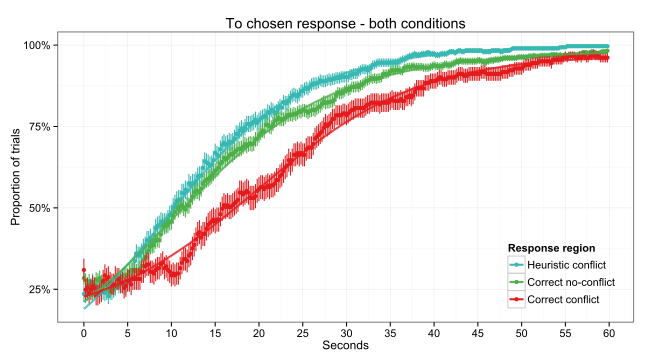
\includegraphics[width=\figurewidth]{imgs/exp6-all-to-chosen.pdf}
  \caption[Proportion of cursor in region of chosen response option, Experiment 6.]{
    \label{fig:exp6-all-to-chosen}
    Proportion of mouse cursors in the region of
    the response option which was ultimately selected on that trial.    
  }
\end{figure}

This time course data also allows us to
supplement the response time analyses reported above
by looking at the speed at which participants moved the mouse cursor to
the region of the response option they eventually did select.
Figure 4 shows this measure for correct responses to no-conflict problems,
and for both heuristic and correct responses to conflict problems.
The curve for each response region over time
was modelled using third-order polynomial logistic regression models
\citep[or growth curves; see][]{Mirman2014},
such that the log odds of the cursor being in that region were given as
$\alpha + \beta_1 t + \beta_2 t^2 + \beta_3 t^3$.
Natural polynomials were used,
meaning that the intercept corresponded to the log odds at 0 seconds,
the linear term to the simple change over time,
and the quadratic and cubic terms to higher-order 'wiggles' later in the time course.%
\footnote{
  One disadvantage of using these natural polynomial terms
  is that they are by definition correlated,
  and so the model suffers from mild multicollinearity,
  which leads to some loss of statistical power.
  However, as the alternative, orthogonal polynomial terms
  would be difficult to interpret individually,
  I believe this approach lends itself
  to a clearer description of the data.
  }

To test for a significant difference between two curves,
a null model, in which the  weights were the same for each curve,
was compared with a full model, in which there were different  weights for each curve.
Chi-squared tests were used to compare the deviance of each model,
with degrees of freedom corresponding to the number of  parameters added in the full model.
Note that $\alpha$, the intercept, was not allowed to vary between curves.
Finally, a random effect for the linear time term was included for each participant,
to allow for individual variability in
how quickly each participant moved towards a response in general.
Random effects on other terms, by participant, or by problem, were considered,
but led to convergence issues, and so only this term,
which was found to account for the most variance, was included.

Mirroring the response time analyses, and as predicted by all dual process accounts,
participant were faster to move towards
the heuristic response option when selecting it
than the correct option for conflict problems
($\chi^2$ = 4515.7, DF = 3, p < .0001),
with the curves differing significantly on the linear, quadratic, and cubic terms
(z's > 5, p's < .0001; see Figure~\ref{fig:exp6-all-to-chosen}).
Again consistent with the response time analyses,
and contrary to previous findings supportive of the intuitive logic model,
participants were faster to move towards the heuristic response on conflict problems
then to move towards the correct response on no-conflict problems
($\chi^2$, DF = 3, p < .0001).
This effect was mainly driven by a significant difference
on the linear term between the curves (z = 2.352, p = .0187).

Most dual process theories, including default-interventionist,
parallel-competitive, and intuitive logic accounts,
would predict that participants should be
drawn towards the heuristic option
on trials where they ultimately give the correct response.
In order to test for this attraction,
I compared the probability over time of
the cursor being in the region of the heuristic option
with the average probability of it being in the region of
either foil option on those trials (Figure~\ref{fig:exp6-correct-not-chosen}).
A higher probability of being in the region of the heuristic option
than the foils constitutes evidence of an attraction towards that heuristic response.
Visual inspection of Figure~\ref{fig:exp6-correct-not-chosen} shows that
this is the case from approximately 10 seconds onwards.
Again, third order polynomial regression models were fit to this data,
which showed that the difference between the curves was statistically significant
($\chi^2$ = 428.2, DF = 3, p < .0001),
with significant differences on the linear, quadratic, and cubic terms
(z's > 2.1, p's < .05).
Therefore, when selecting the correct response,
participants were more drawn to the heuristic option than to the foils,
as predicted both by default-interventionist
and parallel-competitive or intuitive logic accounts.

\begin{figure}[pt]
  \centering
  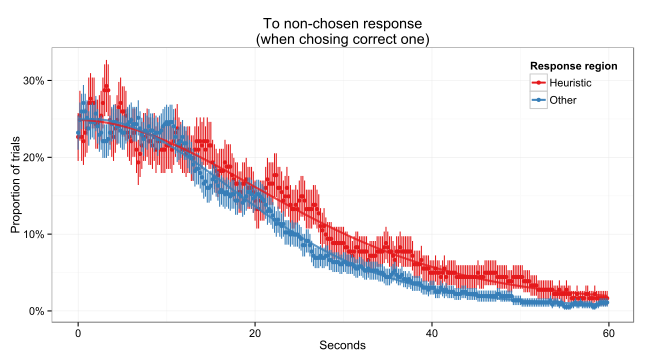
\includegraphics[width=\figurewidth]{imgs/exp6-correct-not-chosen.pdf}
  \caption[Proportion of cursor in region of other response options
  when correct response was given, Experiment 6.]{
    \label{fig:exp6-correct-not-chosen}
    Proportion of trials in the region of each option, over time,
    for trials in which the correct option was eventually chosen,
    for conflict problems.
    Error bars show standard error of measurement.
    Lines show fitted polynomial regression curves.
    Participants were more likely to be in the region of the heuristic response from around 10 seconds onwards.
  }
\end{figure}

\begin{figure}[pb]
  \centering
  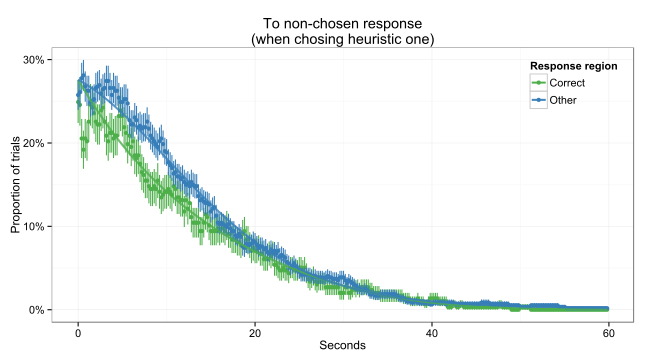
\includegraphics[width=\figurewidth]{imgs/exp6-heuristic-not-chosen.pdf}
  \caption[Proportion of cursor in region of other response options
  when heuristic response was given, Experiment 6.]{
    \label{fig:exp6-heuristic-not-chosen}
    Proportion of trials in the region of each option, over time,
    for trials in which the intuitive option was eventually chosen,
    for conflict problems.
    Participants were less or equally likely to be
    in the region of the correct option than a foil throughout.
  }
\end{figure}


A more interesting comparison is between
the attraction towards the correct response option,
and that towards the foil options,
on conflict trials where the heuristic response is given.
According to the default-interventionist account,
Type 2 processes have not become engaged at this point,
and so the correct response option should not be
any more attractive than the foil options.
According to the parallel-competitive account,
on the other hand, both Type 1 and Type 2 processes
should be engaged on such trials,
and so participants should be drawn towards
giving the response cued by Type 2 processes
(that is, the correct response).
Either result could be consistent with the intuitive logic theory,
depending on the mechanism by which conflict is actually detected.
If conflict detection occurs because
Type 1 processes simultaneously cue both the correct and heuristic responses,
then attraction towards the correct response option should be seen here.
Conversely, if conflict is detected
without Type 1 processes actually producing the correct response,
then the intuitive logic theory,
like the classic default-interventionist account,
would predict no attraction towards the correct response option here.
Of course, no conflict would be predicted by a selective theory.

Figure~\ref{fig:exp6-heuristic-not-chosen} shows that,
contrary to the prediction of the parallel-competitive
and intuitive logic accounts,
participants are not more likely to move towards the correct response option
than either of the foils before giving the heuristic response.
Participants were in fact less likely
to be in the region of the correct option than the foils.
The polynomial regression model showed that
the difference between the curves shown is again significant
($\chi^2$ = 208.0, DF = 3, p < .0001),
with significant differences between the curves on the
linear, quadratic, and cubic terms (z's > 9, p's < .0001).
This result indicates that the correct responses were on average
actually less attractive than the foils.
This is perhaps unsurprising,
given that part of the difficulty of the CRT
lies in the failure of intuition to support the correct response.

%% Finally, once again following previous tests of
%% the intuitive logic theory \citep[e.g.][]{Mevel2014},
%% I repeated the time course analyses reported above for both the
%% ``majority heuristic'' and ``minority heuristic'' participants.
%% The plots for these analyses are shown in Appendix~\ref{appendix:exp6_participants},
%% and reveal that my main findings hold for
%% both sets of participants.
%% \aside{This bit is tricky, especially after the reviews.
%%   Talk about by-item differences here?
%%   Eye balling them, there really is no difference for the bat and ball problems,
%%   but maybe I could test this?}
%% Appendix~\ref{appendix:exp6_items} shows the same analyses
%% plotted separately for each of the eight CRT problems.
%% Again, the results described broadly hold true across all items.
%% However, the bat-and-ball question
%% can be seen to differ slightly from the others
%% in some of the analyses here.
%% I explore this discrepancy in Appendix~\ref{appendix:exp6_items_model}.

\FloatBarrier


\section{Discussion}

These results are broadly consistent with
a default-interventionist dual process theory
\citep{Evans2006,Kahneman2005}.
On problems with an incorrect but intuitively appealing heuristic response,
this response was given more quickly,
and with less evidence of conflict,
than the correct response.
Participants began to systematically move the mouse cursor
to the region of the heuristic response option within approximately 5 seconds,
compared to 10 seconds for movements to the correct response option,
and this trend was evident both when analysing all trials,
and trials in which the response in question was given.
This also appears to be true of both biased and unbiased participants. 

When participants did give the correct response on these conflict problems,
they spent more time in the region of the heuristic response option
than either of the foil options before doing so ---
a finding consistent with default-interventionist,
parallel-competitive, and intuitive logic accounts,
suggesting that these participants considered the heuristic response
before they reached the correct one.
This finding is also consistent with modelling work
\citep{Bockenholt2012,Campitelli2013},
and individual differences studies \citep{Liberali2012}
which have shown that inhibition of the heuristic response
is an important predictor of accuracy on the CRT.
However, contrary to the prediction made from
a parallel-competitive dual process theory
\citep{Sloman1996,Sloman2014}
or by the intuitive logic account
\citep{DeNeys2014a,DeNeys2012,Handley2015}
on trials where the heuristic response was given
participants were no more likely to place the cursor
in the region of the correct response option than either foil option.

These results also have implications for the logical intuitions theory
\citep{DeNeys2012,DeNeys2014a}.
First, a number of previous studies using simpler reasoning tasks
have found that heuristic responses to conflict problems take longer
than correct responses to no-conflict problems,
despite both being cued by Type 1 processes
\citep{DeNeys2008,Stupple2008}.
To my knowledge, the current study is the first to report response times
for conflict and no-conflict versions of the CRT,
and although this analysis was not the main focus of the this experiment,
I found no such effect.
In fact, when analysing participants speed of movement
to the response option they ultimately selected, a more sensitive measure,
I found the opposite effect,
with participants faster to move to the heuristic option under conflict
than the correct option for no-conflict problems
on trials where these responses were given.
All of these findings were true for both
participants who gave the heuristic response to most conflict problems,
and those who did not.
Thus, unlike a number of studies using simpler reasoning problems,
I found no evidence that participants were slower
to give intuitively-cued responses which were wrong
than intuitively-cued responses which were right.

Secondly, as discussed above, I found no evidence of
an attraction towards the correct response option
on conflict problems where the heuristic response was given.
This suggests that Type 1 processes did not simultaneously
cue both responses on such trials.
This result is not, however, totally inconsistent with the logical intuitions theory.
Previously, I differentiated between
a dual process conflict monitoring account \citep{DeNeys2008,DeNeys2008a},
that proposes that we detect when our reasoning is biased,
and a fully-fledged intuitive logic theory \citep{DeNeys2012,DeNeys2014a,Handley2015},
where this conflict detection is the result
of Type 1 processes simultaneously cuing
both the correct and the heuristic response.
These results would appear to contradict the latter account,
%% \citep{DeNeys2012,Handley2015,Pennycook2015,DeNeys2014a}
whereby Type 1 processes cue both the heuristic response (``10p'')
and the correct response (``5p'') at the same time
for the bat-and-ball problem and other CRT items.
They do not, however, rule out the possibility that
participants experience uncertainty \citep{DeNeys2013a},
or a feeling of wrongness \citep{Gangemi2015}
while solving these conflict problems.
If this is the case, further work is needed to reveal how this feeling comes about.

At this point, I would like to note again that,
\citet{DeNeys2013a} and \citep{Gangemi2015} notwithstanding,
previous evidence for the intuitive logic theory has come from simpler experiments,
such as simple syllogistic reasoning \citep{Morsanyi2012}
and forced-choice base rate neglect \citep{DeNeys2008} paradigms.
The operations required to reach the correct answer to these CRT problems
are considerably more complex than those needed to evaluate a simple syllogism,
or apply basic statistical principles.
Therefore, while I do not find evidence that Type 1 processes
automatically generate correct responses on the CRT,
this does not rule out the possibility that they can
generate correct responses on these simpler tasks.
For instance, it has been demonstrated that participants
report ``liking'' syllogisms which are logically valid
more than those which are invalid,
even when not asked to evaluate their logical status \citep{Morsanyi2012},
but also that this effect only holds for simpler logical forms
\citep[see also \citealp{Handley2015}]{Klauer2013}.
Indeed, \citet{DeNeys2012},
when proposing the intuitive logic account
raised the possibility that it
may not apply to all problems.
%% With this in mind, it is worth considering if
%% the reductions in confidence for conflict problems reported by
%% \citet{DeNeys2013} and \citet{Gangemi2015} can be explained
%% without recourse to logical intuitions.
%% One possibility is that participants were engaged in \emph{rationalisation}
%% \citep{Ball2003,Evans2006,Pennycook2015}.
%% That is, while Type 1 processes cued initial responses,
%% participants in both conditions may engage shallow Type 2 processes
%% to attempt to verify them.
%% For no-conflict problems, participants can easily verify
%% that their intuitive response is correct,
%% and so give it with confidence.
%% For conflict problems, on the other hand,
%% their initial responses would be incorrect,
%% and so they would not be able to validate them.
%% Some participants would give these unvalidated responses,
%% but lack confidence in doing so,
%% while others would engage further Type 2 processes to produce the correct response.
%% Crucially, such an account would not require that
%% participants implicitly detect the error in their initial responses.
%% This account should also be testable in future.
%% If the reduction in confidence is the product of an implicit detection of conflict,
%% it should occur early in the reasoning processes.
%% Alternatively, if it is the product of
%% an inability to explicitly validate an intuitive response,
%% the reduction in confidence should occur later,
%% after these shallow Type 2 processes have been engaged.
%% I would stress at this point, however,
%% that I do not dispute the validity of the intuitive logic theory more broadly here,
%% but rather question if it applies equally to complex logical tasks as to simple ones.

One might argue that the absence of evidence for either
the parallel-competitive or intuitive logical theories here
do not reflect evidence against these accounts,
but rather the inability of this paradigm to reveal
the effects predicted  by these accounts.
It may be the case, according to this line of reasoning,
that participants are drawn towards the correct option
on trials where they give the heuristic response,
or that participants are more conflicted
when their heuristic responses are wrong than when they are right,
but that I was unable to detect these mental states using this new paradigm.
While I cannot completely rule out this possibility,
I believe two factors go against such an interpretation.
First, this paradigm does reveal effects,
such as attraction towards the heuristic option before giving the correct response,
consistent with the default-interventionist model.
Second, for the two comparisons above, rather than finding no effect,
I found significant effects in the opposite direction
to those predicted by parallel-competitive and intuitive logic accounts.

Additionally, there is extensive evidence that
even subtle, implicit cognitive processes
influence motor output in detectable ways
\citep{Tucker2004,Xiao2014,Miles2010,Bargh2006}.
Therefore, if participants do experience conflict,
but this conflict does not influence their motor output,
then this raises the question of
what  mechanism produces this conflict
while not influencing motor output.
I return to this issue in Chapter 7.
Finally, I would note again that these results
should be interpreted as
constraining the intuitive logic account,
rather than falsifying it.

Of course, all of the above assumes a dual process interpretation of the CRT,
as most treatments of the task do.
Even in accounts which focus instead on dispositional factors
\citep{Campitelli2013,Campitelli2010a},
it is acknowledged that responding correctly typically requires
the inhibition of the heuristic response.
While I am unaware of any accounts of the CRT
which do not rely on such an inhibition,
I cannot rule out the possibility of such explanations being offered in future.
The current results, however, provide an additional constraint to such accounts,
in that they should predict not only observed choices,
but also the patterns at the process level reported here.

As a side note, it may be noted that it is unusual
to present the CRT as a multiple-choice test,
and that this may affect the processes engaged during this experiment.
However, multiple-choice versions for the test have been previously reported
by \citet{morsanyi2014mathematical}, \citet[][Experiment 3]{Primi2015},
and \citet[][Experiment 2]{Gangemi2015},
without any clear effect on participants’ responses.


Finally, since its introduction in 2005, the CRT has been hugely popular
as a measure of individual differences in thinking,
despite only limited evidence as to what underlies performance on the task.
These results go some way towards filling this gap,
and suggest that responding correctly
does require the activation of otherwise dormant Type 2 processes
to override incorrect intuitions.
Future work might address the relationship between
conflict on this task and individual differences.
\citet{Stanovich2008} proposed that normative decision making requires
(1) awareness of the limitations of intuition;
(2) desire to overcome those limitations;
(3) inhibition of the intuitive response and
(4) ability to generate the correct response.
Each of these requirements is a distinct reason for
failure to produce the correct response on the CRT,
and each should produce a distinctive pattern in mouse cursor movement data.

To conclude, I recorded participants' mouse cursor movements
over a considerable period of time
while they reasoned about CRT problems.
Trends in these movements were consistent with
a default-interventionist dual process theory of reasoning,
where participants are initially drawn towards heuristic responses only,
but in some cases engage further effortful processing to find correct solutions.
I did not find evidence that participants were
drawn to correct responses on trials where these responses were not actually given,
inconsistent with a parallel-competitive dual process account.
Finally, contrary to previous work using simpler reasoning tasks,
and confidence ratings collected on the CRT,
I found no evidence that participants were conflicted
when giving incorrect heuristic responses. 




\chapter{Summary, Discussion and Final Conclusions}
\graphicspath{{7.Conclusions/}}
\section{Recapitulation}\label{sec:ch7-recap}

In this thesis, I have used the mouse tracking paradigm
across a series of experiments to investigate conflict in reasoning.
In doing so, I hoped to further understand
under what circumstances conflict arises,
what form this conflict takes,
and at what points in time it occurs.

In Experiments 1 and 2 (Chapter 3),
I pitted perceptual cues in the form of visual similarity,
against conceptual knowledge in the form of category membership,
in a forced-choice induction task,
using both natural (Experiment 1) and artificial categories (Experiment 2).
In both experiments, I found that
perceptual cues are an early driver of participants' motor output,
and that conceptual knowledge is brought online later in reasoning,
sometimes causing participants to change direction
if they had begun to move towards the perceptually-cued option.
Analysis of the time course data showed that
participants began to be drawn towards
the perceptually-cued foil from 300 msec (in both experiments),
and did not begin to inhibit this attraction until \tildetext750--1,500 msec.
In Experiment 2, I further showed that participants were more likely
to override their perceptually-driven movements
when reasoning about properties that were conceptually related
to the distinction between the categories,
likely because these properties make conceptual knowledge more accessible,
or help participants realise that the perceptual cues were inappropriate.
Again, this effect, being dependent on conceptual knowledge,
was not visible until \tildetext620 msec.

Experiments 3 and 4 (Chapter 4) were similar,
but pitted associative knowledge against structured knowledge.
In Experiment 3, I contrasted conflict trials,
where the foil response was strongly associated with the base
according to separate association ratings,
to control trials, where it was not.
In Experiment 4, I collected association ratings
from each participant for each pair of species.
This allowed me to conduct regression analyses
with both each participants' associative knowledge
(the ratio of the association ratings in favour of each response)
and structured knowledge as predictors.

In both experiments, I again found that participants were
influenced by both kinds of information:
in Experiment 3 participants gave the correct response
on \tildetext95\% of control trials but only \tildetext75\% of conflict trials,
while in Experiment 4 both structured and associative knowledge
were significant predictors of participants' responses.
However, compared to the previous experiments,
there was less evidence here that participants were
initially drawn towards the associatively-cued option,
and then subsequently towards the structured response.
While this did happen on some trials,
on most trials participants either moved straight to one response option,
or straight to the other.

In Experiments 5 and 6,
I explored conflict from the perspective of
dual process theories of reasoning.
In Experiment 5 (Chapter 5),
participants completed a mouse tracking version of
the base rate neglect task \citep{Kahneman1973,DeNeys2008}
where they could draw on either stereotypical descriptions
or statistical base rates to decide someone's social category.
I manipulated both the descriptions and the base rates,
so that they could either agree, disagree,
or only one cue was informative.

Consistent with a default-interventionist dual process model \citep[i.e.][]{Evans2006},
I found that participants' responses were predominantly determined by
the contents of the descriptions,
and that participants who opted to ignore the description
and rely on the base rate instead experienced conflict.
In line with previous work \citep[e.g.][]{Tversky1982,Kahneman1973},
but counter to intuitive logic accounts \citep{DeNeys2008,Pennycook2014}
or a parallel-competitive dual-process account \citep{Sloman1996},
the influence of the base rates was less pronounced.
Specifically, participants did sometimes give the base rate-cued response
even when it conflicted with the description (\tildetext20\% of trials).
Aside from this, however,
participants responding on the basis of the descriptions
did not show signs of conflict when the base rate was manipulated
to disagree with the description.
A Bayesian follow-up analysis, finally,
showed that despite the non-significant effect,
there was not considerable evidence for the existence of a null effect either.
Rather, it seems that participants were
very slightly (\tildetext 3\%, or around 30 msec) slower
giving the description-cued response
when it disagreed with the base rate.

In Experiment 6 (Chapter 6),
participants completed the more complicated
Cognitive Reflection Test \citep[CRT;][]{Frederick2005}:
a series of questions for which
the first response that comes to mind is often incorrect.
Unlike Experiments 1 to 5,
there were four response options here,
located in each corner of the screen.
Participants were allowed to respond in their own time,
and I analysed movements of the mouse cursor
over the first sixty seconds of each trial
as  participants moved the mouse around the screen deciding on a response.
This novel form of mouse tracking
made it possible to record participants' ongoing decisions over a longer period of time.
It also allowed me to infer participants' attraction towards four response options,
rather than the two used in standard mouse tracking.
This was useful in differentiating between
effects where participants are actually drawn
towards a particular alternative response option,
and those where participants are merely slow
to move towards the option they do choose.
I also included, following \citet{DeNeys2013a},
no-conflict versions of the CRT problems
to serve as a control condition where
participants' first, heuristic responses are the correct ones.
Finally, this experiment was, to my knowledge,
the first to record response latencies on any version of the CRT.

Consistent with a dual process perspective,
heuristic responses on the CRT were given more quickly,
and participants were faster to approach these response options before selecting them,
than correct options.
Contrary to response time analyses of other tasks \citep[e.g.][]{DeNeys2008}
and confidence rating data from the CRT \citep{DeNeys2013a,Gangemi2015} however,
participants were no faster to give
the heuristic (and correct) response on no-conflict problems
than to give the heuristic (and incorrect) response on conflict problems.

The nature of the mouse tracking data here allowed for a number of novel analyses.
First, I demonstrated that on conflict problems
participants began to be drawn towards the heuristic option from 3.7 seconds,
and towards the correct option from 9.3 seconds,
including time spent reading the problems.
More relevantly, to test for the presence of conflict
I calculated, for trials where participants gave one response,
the degree to which their mouse cursor was in the region of
the alternative, competitor response beforehand,
compared to the regions of the other two non-competing responses.
Thus, for instance, if a participant giving the correct response
is drawn towards the heuristic option while doing so,
their cursor will spend more time in the region of the heuristic option,
on average, than either of the other two foil options.
Again in line with a default-interventionist model,
I found exactly this effect,
as participants were drawn towards the heuristic option
before selecting the correct one.
However, contrary to some other accounts, the reverse was not true:
participants did not hover over the correct option
before ultimately selecting the heuristic one.

In this final chapter,
I try to make sense of these results
and discuss the implications they have for what we know about conflict in reasoning.
I do this both within the specific sub-domains
that these experiments addressed ---
information selection in induction,
and dual process theories of reasoning ---
and in terms of conflict in reasoning and cognition more broadly.


\section{Conflict in Reasoning}\label{sec:ch7-conflict}

It is clear, both from this thesis and from a wealth of previous work
\citep{DeNeys2012,Crisp-Bright2010,Botvinick2004a,Miller2001},
that conflict in cognition arises in many places.
In Chapter 1, I introduced two particular junctures:
conflict between competing representations in induction,
and conflict between Type 1 and Type 2 processes.
At this point, it is worthwhile considering
how these two forms of conflict fit into
the broader scope of the interacting processes
that underlie reasoning.

I propose that
both kinds of conflict
can be understood in terms of
the role of working memory in reasoning,
and the interaction of working memory-based processes
with other cognitive processes.

Some cognitive functions
are almost certainly achieved by
fast, associative, processes.
Typical, but not defining properties of these processes are that
they are autonomous (they operate automatically
when presented with their triggering cues),
they are associative (rather than rule-based),
they generally operate quickly,
and are not cognitively demanding.
In dual process accounts of cognition,
these are known as Type 1 processes
\citep[or, in the past, as \emph{System 1}; e.g.][]{Sloman1996}.
\citet{Stanovich2005,Stanovich2009}, highlighting the diversity of these processes,
labels them the \emph{Autonomous Set of Systems}.
In his definition of this set of processes,
\citet{Stanovich2009} includes
both domain specific evolved \emph{modules},
and general learned associations,
which have become autonomous through practice or repeated exposure.
While some of these Type 1 processes serve to
provide information to other cognitive process,
including for use in more effortful, deliberate cognition,
others can affect our actions directly
without being mediated by other processes.


Clearly, under this definition, many cognitive processes are autonomous.
To fully catalogue these processes would take a lifetime,
and so for the purpose of this discussion
it suffices to say that there exist a constellation of processes
that are generally fast, associative, and autonomic.
Well-known such processes include face recognition
\citep[largely an evolved processes,
  localised to the fusiform gyrus;][]{Kanwisher1997},
reading text \citep[a learned skill
  that maps onto the left fusifom gyrus;][]{McCandliss2003},
and word recognition \citep[e.g.][]{Spivey2005}.

%% %% %% %% %% %% %%% 
%% Here be Dragons %% 
%% %% %% %% %% %% %%% 

%% Aidan: given John's concerns, I think that you need something here
%%    where you first talk about Type 2 processes and how the thing that
%%    distinguishes them from Type 1 processes is that they rely on Working
%%    Memory. The importance of WM to current dual process frameoowrks will
%%    allow you to attempt to resolve the various findings in your
%%    thesis....and then you can proceed from there. Otherwise, John is
%%    right, you look like you are taking a theoretical turn that you
%%    haven't advertised or prepared the reader for.

%% 

%% \aside{From Evans and Stanovich (2013)
%%   The definition of Type 2 processing:
%%   The large literatures on working memory and executive function
%%   (Baddeley, 2007) have established that there is a general purpose
%%   system used in many higher cognitive functions and that the capacity
%%   of this system varies reli- ably between individuals. [\ldots]  It is
%%   the engagement of this system specifically that Jonathan Evans
%%   (e.g., 2008, 2010a) has emphasized in the definition of Type 2
%%   processing and which underlies many of its typically observed
%%   correlates: that it is slow, sequential, and correlated with
%%   measures of general intelligence. [\ldots]  Stanovich (Stanovich, 2011;
%%   Stanovich \& Toplak, 2012) has also strongly emphasized the features
%%   that he calls “cognitive decoupling” in his definition of Type 2
%%   processing. This is again compatible with Evans’s (2007a, 2010b)
%%   view that such processing is necessary for hypothetical thought. In
%%   order to reason hypothetically, we must be able to prevent our
%%   representations of the real world from becoming confused with
%%   representations of imaginary situations. The so-called cognitive
%%   decoupling operations are the central feature of Type 2 processing
%%   that makes this possible according to Stanovich (2009b, 2011).
%% }

%% \aside{
%%   The definition of Type 1 processing: 
%%   We both agree that the defining characteristic of Type 1 processes is
%%   their autonomy. They do not required ``controlled attention'', which
%%   is another way of saying that they make minimal demands on working
%%   memory resources.}
%% 
%% }

Other processes, however,
require the sustained representation,
maintenance, and manipulation of information in working memory,
\emph{decoupled} from interference from
competing Type 1 processes \citep{Stanovich2008,Evans2013a,Gilbert1991}.
More recent dual process accounts
\citep[see][]{Evans2013a,Stanovich2012,Evans2004}
propose that this decoupling in working memory
is the defining feature of Type 2 processes.
In this account, Type 1 processes, in contrast,
are simply those that are \emph{autonomous},
or do not require controlled attention or working memory resources
\citep[p. 236]{Evans2013a}.

These Type 2 processes,
making use of working memory,
have the advantage of being extremely flexible.
Many Type 1 processes are thought to be \emph{domain specific} \citep[see][]{Cosmides1994a},
in that they are restricted to processing only one kind of information.
An archetypal example of this is the process responsible for face perception,
a small system localised to the bilateral fusiform gyri
\citep[or \emph{fusiform face areas; }see][]{Kanwisher1997}.
This system is exquisitely well adapted to recognise human faces in visual input,
but when presented with other stimuli will either not activate,
or mistakenly indicate that it has seen a face.%
\footnote{
  The common illusion of perceiving faces
  in non-facial stimuli is known as pareidolia.}
Type 2 processes, however, are \emph{domain general},
and can equally well process information about faces, words,
geographical locations, and abstract concepts.
These processes are also thought to be unique
in their ability to sequentially apply rule-based operations
\citep{Cooper1973,Anderson2014,Anderson1996a},
in contrast to Type 1 processes, which are thought to
work on associative principles \citep[see][]{Sloman1996}.
This flexibility comes at the cost, however, of limited capacity.
Working memory capacity
--- and thus the capacity of Type 2 processes ---
is limited first of all in that, compared to Type 1 processes,
through which an enormous amount of information streams in parallel,
only a very small amount of information can be held
in working memory at one time
\citep[famously 7 chunks of information, $\pm$ 2, according to][]{Miller1956}.
Working memory is limited secondly in that
many theories hold that only one state of the world,
or mental representation,
can be held in working memory at any one time.
This means that we can consider one possible mental representation,
followed by another, but that we cannot simultaneously consider
two contradictory representations.
This limitation has been noted across a number of research traditions,
including in dual process theories as the
\emph{singularity principle} \citep{Evans1984,Evans2006},
in mental models accounts of reasoning \citep{Johnson-Laird1983}
as \emph{focusing} \citep{Legrenzi1993},
by those interested in diagnosis as an inability to
consider more than one hypothesis at a time \citep{Mynatt1993},
as well as in the literature on working memory itself \citep{Baddeley2007}.

My proposition is as follows.
First, the inductive triad tasks used in Chapters 3 and 4
require that participants hold
the three categories presented in working memory,
to compare the inductive potential from the base
to each of the candidate responses.
To do this, they must draw on information
about the relationships between the categories shown.
This information, naturally, must come from elsewhere,
and in these tasks it can come from a number of Type 1 processes:
from the visual system, for instance,
or from different aspects of long term memory \citep{Jackson2015},
including both associative and structured knowledge.
As only one representation of the world
can be held in working memory at a time,
conflict arises when multiple Type 1 processes
provide multiple contradictory representations.
I contend that the induction tasks reported here
involve conflict in this sense,
as representations based on perceptual cues or conceptual knowledge
(Experiments 1 and 2),
or on associative and structured knowledge (Experiments 3 and 4)
vie to be realised.

Second, there are some problems for which responses can be cued
either by Type 1 processes,
operating on associative principles and placing few demands on working memory,
and by Type 2 processes
that involve maintaining information in working memory
while applying sequential, rule-based operations.
These are, of course, the problems addressed by
dual process theories of reasoning.
\citep[e.g.][]{Evans2013a,Evans2008,Kahneman2011}.
I investigated two such problems in this thesis:
reasoning about base rates and stereotypes (Experiments 5),
and the Cognitive Reflection Test (Experiment 6).
My account for performance on these tasks
is no different from the generic dual process account.
On the base rate task, Type 1 processes
are responsible for processing the descriptions,
and automatically cue stereotype-consistent responses.
To process and respond on the basis of the base rates, however,
one must engage Type 2 processes to relate
the statistical information to the task at hand and choose a response
(and, under most accounts, to inhibit the description-cued response).
Similarly, on the CRT,
Type 1 processes automatically cue incorrect heuristic responses,
without the need for sustained Type 2 processing.
To reach the correct response, however,
participants must represent the problem in working memory
and apply the rules of arithmetic, an archetypal Type 2 operation.

\begin{figure}[ht]
  \centering
  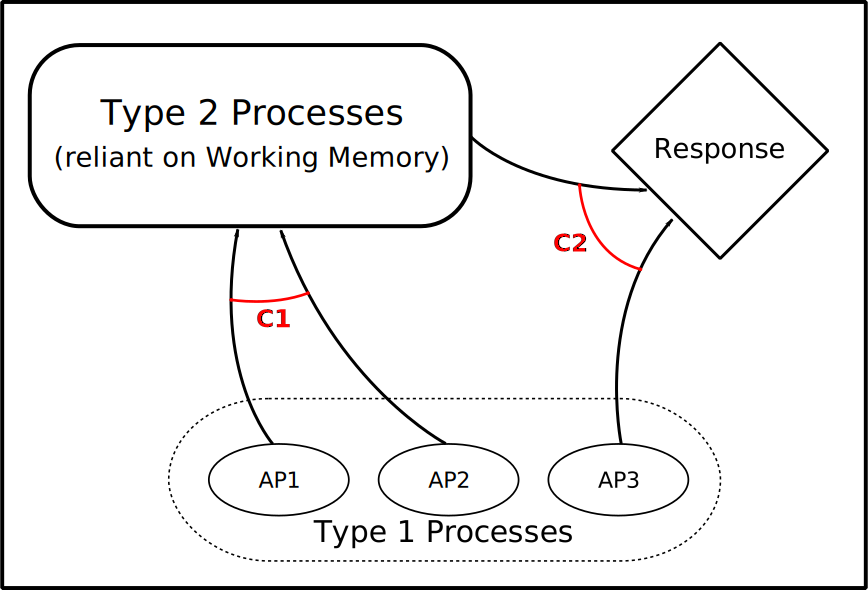
\includegraphics[width=\figurewidth]{imgs/simple-framework.pdf}
  \caption[A framework for conflict in reasoning]{
    \label{fig:conflict-framework}
    A simple framework for conflict in reasoning.
    Reasoning requires the interaction of
    associative, Type 1 processes (AP1, AP2, AP3, etc.),
    and Type 2 processes, reliant on working memory.
    Conflict in reasoning arises
    a) when multiple Type 1 processes
    attempt to project information to working memory
    (\textcolor{red}{C1}), and
    b) when both Type 1 
    and Type 2 processes attempt to produce responses
    (\textcolor{red}{C2}).
    I propose that conflict of type \textcolor{red}{C1} occurs
    when multiple sources of information,
    such as perceptual cues, associative knowledge, or structured knowledge,
    are available during inductive reasoning.
    Conflict of type \textcolor{red}{C2}, conversely,
    occurs in reasoning when both Type 1 and Type 2 processes
    can generate responses, for instance description
    and base rate-cued responses in Experiment 5,
    or heuristic and correct responses in Experiment 6.
  }
\end{figure}

Figure~\ref{fig:conflict-framework} shows a simple sketch of
this framework for thinking about conflict in reasoning.
In short, conflict can arise both
as multiple Type 1 processes attempt to project information to working memory,
or because both Type 1 and Type 2 processes
attempt to produce responses to the same problem.
With this framework in mind, I now return to the interpretation of my results.


\section{Knowledge and Reasoning}\label{sec:label}

%% Leaving aside this broader framework for a moment,
%% my results have particular implications
%% for a number of theories of inductive reasoning in particular.
In Experiments 1 and 2 (Chapter 3) and 3 and 4 (Chapter 4),
I looked at what information people drew on during inductive reasoning,
using triad tasks.
In these, participants were asked to project a property
from a base category, known to have the property in question,
to one of the two other categories.
Above, I argued that this task requires that participants represent
the three categories in working memory,
and then draw on information about each category
to decide to which of the two response categories the property likely generalises.
Thus, the framework above provides
a mechanistic account of the operations proposed
by \citegap{Bright2014a}{'s} hybrid theory of induction.

In Experiments 1 and 2,
I pitted perceptual cues against conceptual knowledge,
and in Experiments 3 and 4,
I pitted associative knowledge against structured knowledge.
An interesting question that arises at this point, therefore,
is if these two kinds of conflict really unfold in the same way.
In Experiments 1 and 2, the interaction of
perceptual cues and conceptual knowledge was straightforward:
perceptual cues drove participants' motor output early in reasoning,
and conceptual knowledge was retrieved later,
causing participants driven towards the foil response
to sometimes change direction to select the right one instead.
In Experiments 3 and 4 the picture was less clear.
On the one hand, participants did sometimes initially move towards the foil option
before giving the correct response,
and a greater proportion of correct responses were reversals under conflict.
On the other hand, these reversals were considerably rarer
than in Experiments 1 and 2,
as participants for the most part moved towards one other response option,
and then selected it.

These differences can be captured by two of the parameters
in my analysis of the transition probabilities of cursor trajectories:
$1 - \alpha$, the probability of initially moving towards the foil option,
which was higher for perceptual cues (\tildetext50\%)
than for associative knowledge (\tildetext35\%),
and $\gamma$, the probability of overriding an initial movement towards the foil,
which was again higher for perceptual cues (\tildetext50--80\%)
than associative knowledge (\tildetext25--35\%).

One possibility here is that
the differences between the two sets of experiments are only quantitative.
It may be that participants are very prone to
draw on perceptual cues during reasoning,
but that they are also relatively good at
overriding the influence of these cues,
doing so, at minimum, on 50\% of trials.
Conversely, it may be that
associative knowledge may only be retrieved some of the time,
but participants who do retrieve this knowledge are
considerably less likely to subsequently inhibit or override it.
From this point of view, the phenomena studied in
both Experiments 1 and 2 and in Experiments 3 and 4
are examples of conflict occurring as different Type 1 processes
attempt to project information to working memory.

An alternative possibility, however, is that
the difference between the two sets of experiments is qualitative.
An extensive body of research \citep[see][for a review]{Goodale2004}
shows that information passes through the human visual system in two streams.
A dorsal stream leads from the visual cortices
to the prefrontal cortex and allows us to
consciously perceive stimuli and to hold them in working memory.
A ventral stream, however, leads directly to the motor cortex
and allows our actions to be informed by perceptual cues
without conscious awareness.%
\footnote{
  In the extreme, damage to ventral system
  can leave individuals able to respond to visual stimuli,
  without being consciously aware of seeing them,
  a condition known as \emph{blindsight} \citep{Weiskrantz1986,Salti2015}
}
It could be the case that
rather than participants seeing the visual cues in Experiments 1 and 2,
representing this information in working memory,
and reasoning from there,
this information may have been passed directly
from the perceptual system to the motor cortex.
In this case, these results could also be interpreted as a dual process phenomenon,
if we allow that this perceptual-action coupling constitutes a Type 1 process.

On the basis of the current data,
it is not possible to differentiate between these two possibilities.
A possible future approach, however,
may be to investigate the relationship between
performance on both of these versions of the triad task
and measures of different kinds of inhibitory control.
According to \citet{Diamond2013},
there are broadly speaking two kinds of inhibitory processes.
One is \emph{response inhibition},
which allows us to override automatically executed motor commands.
The purest (i.e. least confounded by other factors) measures of this kind of control
are the Go/No-Go \citep{Donders1868} and Stop-signal \citep{Lappin1966} tasks.
Both of these require participants to quickly give a response
associated with a given stimulus,
except on trials where a no-go or stop signal is presented.
The other inhibitory process is \emph{cognitive inhibition},
which inhibits and filters out irrelevant or unwanted
mental representations and information.
Of particular relevance here is \emph{semantic} inhibitory control,
a subset of cognitive inhibition measured using the Hayling task \citep{Burgess1997}.
In the non-clinical version of this task \citep{Markovits2004},
participants are primed with incomplete sentences
(e.g. ``The captain wanted to stay with the sinking $\rule{1cm}{0.15mm}$``),
and then shown a single word and asked to indicate if it is an appropriate word
with which to finish the sentence.
Crucially, on lure trials the probe was a pseudo-word
similar to a real word primed by the sentence ---
i.e. ``shifp'' when ``ship'' was expected.
This requires that participants inhibit their automatically primed
semantic knowledge to correctly reject this word.

\citet{Bright} presented participants with the triad task from Experiment 3,
which placed associative and structured knowledge in conflict.
They also collected measures of both response inhibition (the Stop-signal task)
and semantic inhibition (the Hayling task).
Their results showed that the effect of associative knowledge
--- fewer correct responses when associative knowledge cued the foil ---
was more pronounced for participants who performed poorly on the Hayling task
(responded that the lure pseudo-words were appropriate),
but was not related to individual differences in
performance on a Stop-signal task.
Therefore, they concluded that foil responses on this task
are the result of a failure to inhibit
inappropriate semantic knowledge in favour of structured knowledge,
rather than a failure to inhibit the inappropriate response itself.

Applying this logic to Experiments 1 and 2,
I would predict that if foil responses on these tasks
are the result of conflict between representations in working memory
like foil responses in Experiment 3 and 4, and in \citegap{Bright}{'s} experiment,
participants lacking in semantic inhibitory control
should be more likely to err in this way.
Conversely, if these foil responses
are instead the result of a failure to inhibit
the response automatically cued by the visual cues,
it should be participants with poorer response inhibition
that err in this way instead.
Clearly, further research is needed to resolve this question.

Beyond this question, however, the experiments reported in both
Chapters 3 and 4 have implications for theories of induction more broadly.
First, these results are consistent with \citegap{Bright2014a}{'s} argument
that theories of induction that draw on just one kind of knowledge are incomplete.
Instead, it seems that induction can be driven by multiple forms of information.
\citet{Bright2014a} showed that different sources of information are used
depending both on individual differences (semantic inhibitory control)
and on situational factors (the presence of secondary load).
The current results showed that multiple kinds of information
can drive reasoning even within a single trial, leading to conflict.

Formal modelling plays an important role in research on induction
\citep[see, e.g.,][]{Sloman1993,Osherson1990,Kemp2009,Hawkins2015}.
These results, however, are challenging to model using existing frameworks.
A natural next step, following on from \citegap{Bright2014a}{'s} hybrid account,
would be to attempt to model these time course data
using a hybrid of existing models based on associative and structured knowledge.

This could potentially be achieved, for instance,
by a change-point model where reasoning is driven by
one kind of information before time $t$,
and by another model afterwards.
Another potentially interesting avenue here is
the CLARION cognitive architecture \citep[e.g.][]{Sun1995,Sun2006},
which combines implicit similarity-driven
and explicit rule-based operations.
\citet{Sun2006}, for instance, use this architecture
to model performance on a number of inductive reasoning problems.
However,  at present this model does not account for
the time course data presented here,
and so further work would be needed
to model the full temporal dynamics of reasoning.

%% \aside{I'm not totally sure this next paragraph
%%   should be here at all.}
%% Another question that arises is whether or not
%% participants always experience conflict here.
%% While I have said much about the strengths of the mouse tracking paradigm,
%% one obvious weakness is that it only reflects ongoing cognitive processes
%% once participants actually begin to move the mouse.
%% There is unavoidably%
%% \footnote{
%%   Unavoidable unless one uses the approach introduced by \citet{Scherbaum2010}
%%   of only revealing the stimuli once participants begin moving the mouse,
%%   which I found to be unsuitable to reasoning problems.
%% }
%% an interval between participants seeing the trial stimuli
%% and beginning to move the mouse.
%% Therefore, while participants do not initially
%% move the cursor towards the foil on conflict trials,
%% it is not clear if this is because they are
%% genuinely not drawn towards the foil on such trials,
%% or because they are able to inhibit this attraction
%% before initiating their movements.
%% One might expect movement initiation time to be a useful measure here.
%% Unfortunately, the results here were also unclear:
%% there were no effects on initiation time in Experiments 1 and 2,
%% and an effect in Experiment 3, but not 4,
%% despite there being no changes between the experiments
%% that should influence this.
%% However, there is perhaps good reason for movement initiation times
%% to be a confusing index of conflict in cognition.
%% As discussed in Chapter 2,
%% in many tasks, participants are placed under conflict
%% by changing only the identity of the foil option
%% to something towards which participants will be drawn.
%% Therefore, on these conflict trials,
%% participants are drawn towards moving the mouse by two factors
%% --- the pull of the correct option, and the pull of the foil,
%% rather than just the pull of the correct response.
%% Coupled with the pre-emptive inhibition of conflict mentioned above,
%% this may account for the inconsistent initiation time results.
%% However, this leaves unanswered the question of
%% whether or not participants experience conflict on all trials,
%% and so it is a question I must leave open for the time being.






\section{Dual Processes and Reasoning}\label{sec:ch7-dualproc}

In Experiments 5 and 6 (Chapters 5 and 6),
I tested the predictions of dual process theories of reasoning.
At the outset, I introduced a number of types of dual process architecture
outlined by \citet{Evans2007a}:
selective/pre-emptive conflict resolution models,
where reasoners selectively draw on Type 1 \emph{or} Type 2 processes each time;
corrective/default-interventionist models,
where Type 1 processes are activated automatically,
and optionally overridden by Type 2 processes;
and parallel-competitive models,
where both types of process operate in parallel,
and compete for control of behaviour.
I also discussed
what I referred to as
the dual process conflict monitoring account
\citep[e.g.][]{DeNeys2008,DeNeys2008a},
which proposes that participants implicitly detect
that their heuristic reasoning conflicts with normative standards,
and the more recent \emph{intuitive logic} accounts of reasoning
\citep{DeNeys2012,DeNeys2014a,Handley2015},
which propose that this conflict detection happens because
Type 1 processes can simultaneously cue both
biased heuristic responses and normatively correct ones.

These accounts differ in when they predict conflict should occur,
and mouse tracking provides a means of detecting this conflict when it does take place.
Pre-emptive conflict resolution models predict that Type 1 and 2 processes never conflict,
as we selectively activate only one or other kind of process on each task.
Default-interventionist models predict conflict
only when we activate Type 2 processes to override Type 1 responses.
Parallel-competitive models, however, predict conflict to be more common,
as both types of process usually compete to control behaviour.
Like parallel-competitive models, intuitive logic accounts
would predict that we are often conflicted during reasoning,
but while the former claim this is because Type 1 and Type 2 process cue conflicting responses,
the latter claim this occurs because Type 1 processes simultaneously cue multiple responses,
often including both biased heuristic responses and normative correct ones.

Experiments 5 and 6 both tested these various predictions:
Experiment 5 using the base rate neglect paradigm,
where participants responded within five seconds,
and Experiment 6 using the four-alternative Cognitive Reflection Test \citep[CRT;][]{Frederick2005},
where participants were not placed under time pressure.
In both cases, I found results strongly in favour of a default-interventionist model.
First, in the base rate neglect task,
Type 1 processes are traditionally thought to underlie description-driven responses,
and Type 2 processes to underlie base rate-driven responses
\citep{Barbey2007,Kahneman2005,Kahneman2002}.
Participants' early, initial movements were sensitive
to manipulations of the description,
but not to manipulations of the base rate,
as they moved towards the description-cued option
\tildetext66\% of the time, regardless of the base rate.
It was only later in the reasoning process (after 750 msec or so)
that base rates began to influence participants' movements,
and ultimately, some of their responses.
Therefore, it appears that descriptions were processed automatically, by default,
and only in some cases did participants
attend to the base rates and override their default responses.
Also consistent with a dual process interpretation,
when the two cues conflicted participants
overwhelmingly gave the description-cued response,
and were less conflicted while doing so.

In the CRT, similarly,
Type 1 processes are traditionally held \citep{Frederick2005,Kahneman2005}
to drive heuristic responses
(e.g. ``10p'' on the bat-and-ball problem)
whereas Type 2 processes drive correct responses (e.g. ``5p'').
Consistent with this, participants predominantly gave
the heuristic response on conflict problems,
and were faster to do so, showed less signs of conflict,
and were also faster to approach this heuristic response before clicking it.
Analysis of participants' cursor movements also showed that
participants giving the correct response
were more likely to hover in the region of the heuristic option
than any of the other foil options before doing so.
This would indicate that these heuristic responses
must be inhibited before Type 2 processes can produce the correct response.

The dual process conflict monitoring theory \citep[e.g.][]{DeNeys2008,DeNeys2008a},
intuitive logic accounts \citep{DeNeys2012,DeNeys2014a,Handley2015},
and the parallel-competitive dual process theory \citep{Sloman2014,Sloman1996}
make additional predictions about when conflict should occur.
According to the conflict monitoring theory, participants responding heuristically
should show evidence of conflict on problems where
their response is not also the normatively correct one,
compared to problems where it is
(in other words, they show signs of conflict when
their heuristic response is wrong, but not when it is right).
The intuitive logic and parallel-competitive accounts go further,
and propose that this conflict occurs because both
heuristic and correct responses are being cued simultaneously.
The former proposes that Type 1 processes cue both responses
but that the heuristic response, being prepotent, is the one normally given.
The latter proposes that Type 2 processes cue the correct response
at the same time as Type 1 processes cue the heuristic one.

In the two-alternative base rate neglect task,
I tested these predictions by looking to problems where
participants give the description-cued response,
while the base rate either agreed with the description,
was uninformative, or disagreed.
Previous studies \citep[i.e.][]{DeNeys2008a,DeNeys2008,Pennycook2012a,Pennycook2014}
have found that participants are slower to respond
when the description disagrees with the base rate.
Here, I did not find such an effect,
in response times or any other measure ---
although there was not strong evidence in favour of a null effect either.
It appears that participants either
gave the base rate-cued response, or (largely) ignored the base rates altogether.
Therefore, while these results do not support the intuitive logic theory,
they do not falsify it either.

It should be noted, however,
that most studies showing an intuitive logic effect in this paradigm
involved participants responding much more slowly than was the case here.
Therefore, it may be that participants rarely process base rates
when required to respond in less than six seconds (see the Discussion of Chapter 5).
I asked participants to respond quickly in this experiment,
as in Experiments 3 and 4, in order to ensure that
they were still making their decisions while moving the mouse cursor
so that the cursor trajectories would reflect the reasoning process.
In Experiment 6 however,
due to the fortuitous fact that people will
spontaneously move the cursor while inspecting and thinking about
options located around the screen,
I was able to let participants complete the CRT in their own time.

The design of this experiment allowed me to disentangle
the predictions of the dual process conflict monitoring theory
--- heuristic responses to be slower when
they are incorrect than when they are correct ---
from those of the stronger intuitive logic theory,
and of a parallel-competitive dual process model
--- attraction towards the correct option
before selecting the incorrect heuristic option on conflict problems.
However, I not only failed to confirm these predictions,
but in both cases in fact found significant effects in the opposite directions.
Participants were slower to approach the heuristically-cued correct option
on no-conflict problems where it was selected
than to approach the heuristically-cued incorrect option
on conflict problems where it was selected.
Likewise, participants giving the correct response on conflict problems
actually spent \emph{less} time in the region of the correct option
than the other foil options.
However, these results were not predicted by any of the theories considered,
and so were unexpected.
Despite this, it seems that neither the imposition of time pressure
nor a lack of statistical power
can explain the absence of effects
consistent with the intuitive logic theory here.

%% \aside{Link sentence?}


\section{Conflict more broadly}\label{subsec:ch7-broadly}

Aside from the implications of my results
for theories of reasoning,
there is much in this thesis that may be of interest
to those interested in conflict in cognition more broadly.
In this section, I discuss a number of these broader issues.

\subsection{Changes of Mind in Cognition}

In Chapters 1 and 2 (see also Appendix~\ref{appendix:mouse-studies}),
I discussed previous applications of the mouse tracking paradigm.
Most of these studies to date,
studying simple cognitive and perceptual tasks,
have revealed continuous attraction effects,
as participants are partially and simultaneously drawn towards two responses.
However, a number of studies,
mostly of more complex, high-level cognition
\citep[e.g.][]{Dale2011,Tomlinson2013,McKinstry2008,Barca2015}
instead show \emph{reversals}, or \emph{changes of mind}
as participants move first towards one response option,
and then towards the other.
In Experiments 1 to 5 of this thesis, similarly,
I found that my high-level reasoning tasks yielded these changes of mind,
and little evidence of continuous attraction
(see Appendix~\ref{appendix:reversals}).
At present, however, it is not yet clear why
conflict works one way (continuous attraction) for simple tasks,
and another (changes of mind) for more complex ones.

Above, I proposed a simple framework
for thinking about conflict in reasoning.
An important idea here was that,
according to many accounts
\citep{Evans1984,Evans2006,Johnson-Laird1983,Legrenzi1993,Mynatt1993,Baddeley2003},
only one state of the world can be represented in working memory at a time:
it can believe that the correct response is A, or that it is B,
or consider each in turn,
or assign explicit probabilities to each possibility,
but it cannot simultaneously represent
a world where the correct response is A
\emph{and} a world where the correct response is B.
Such fuzzy, graded, partially-overlapping representations, however,
are fundamental to other theories of cognitive function,
including those based on neural networks
\citep{McClelland2014,Rogers2004,McClelland1986a,Hinton2014,Kruschke1992},
sequential sampling models
\citep{Leite2010,Ratcliff2010,Ratcliff1978,Townsend1995,Usher2001},
and dynamical systems \citep{VanGelder1998,Port1995,Spivey2007,Freeman2011a}.
More broadly, there has been philosophical debate as to whether
mental representations in general are discrete and symbolic
\citep{Newell1972,Johnson-Laird1983,Johnson-Laird1991,Dietrich2003},
or continuous, graded, and fuzzy
\citep{Huette2012,Spivey2007,Beer1995,Port1995}.

I propose that continuous graded representations,
and continuous attraction effects,
are the hallmark of processes that do not require
sustained representations in working memory,
or, in other words, of Type 1 processes.
Due to the unique nature of the symbolic,
domain-general processing done in working memory, however,
processes that rely on this (that is, Type 2 processes)
operate in an all-or-nothing fashion:
we ultimately decide that either A or B is the correct response.
Of course, it is possible to explicitly consider uncertainty in the world,
but doing so requires a great deal of cognitive effort
\citep{Murphy2012,Malt1995,Tversky1982}.
Therefore, there is a \emph{symbolic bottleneck} in working memory ---
representations that were continuous and graded
are forced into discrete symbolic states
when they are passed to working memory.
\citet{Dale2005a} provide a formal model
for how continuous and symbolic representations could map onto each other,
using the mathematical framework of \emph{symbolic dynamics}.

This distinction corresponds well with
the claim by \citet{Oaksford2010,Oaksford2012} that
the representations used by Type 1 processes are probabilistic in nature,
while those used by Type 2 processes are approximately symbolic.
It also dovetails with recent experiments
showing that probabilistic tasks that participants normally struggle with
\citep[e.g.][]{Kahneman1979,Murphy2012}
can be solved easily when presented in a way
that allows the inferences to be performed
by perceptual, motor, and low-level cognitive systems
\citep{Chen2013,Glaser2012,Wu2009,Trommershauser2008a,
  Trommershauser2008,Trommershauser2006,Kording2004}
--- or, in other words, by Type 1 processes.
In a similar vein, there is an extensive literature showing
that the human perceptual system routinely solves complex Bayesian inference problems
\citep{Wolpert2005,Kersten2004,Roach2006}
considerably more complex than those
even highly numerate individuals struggle to solve explicitly
\citep[e.g.][]{McNair2013,Barbey2007}.

I predict that changes of mind
should emerge in mouse tracking studies of processes
where Type 2 processes,
involving maintaining and manipulating information in working memory,
are required to produce at least one of the possible responses.
That being said, this is not the only situation
that can give rise to changes of mind.
Changes of mind have been demonstrated, for instance,
when participants move initially
to categorise pseudo-words as real words \citep{Barca2015},
to categorise short-haired women or long-haired  men
as members of the opposite sex
\citep[in contexts where such styles are rare;][]{Freeman2014a},
to respond that scalar implicatures (``some elephants are grey'')
are true, before deciding them to be false \citep{Tomlinson2013},
to ignore the ``not'' in a negated sentence \citep{Dale2011},
as well as when switching between tasks \citep{Hindy2008}.
Of course, while arguments could be made that some of these tasks
can be interpreted from a dual process perspective,
it is also possible that these changes of mind arose from
the interaction of two simple processes, activated one after another,
or even from a single process accompanied by a shift in attention.
My claim therefore is not that changes of mind are
diagnostic of dual processes phenomena
and the engagement of working memory,
but that continuous attraction, and the absence of changes of mind,
are indicative of tasks based only on Type 1 processes.


\subsection{Conflict in the Hand/Conflict in the Mind}

One possible criticism of my findings is that
cognitive conflict may not always have
a measurable effect on moues cursor trajectories.
For instance, the failure of these mouse tracking data
to support the intuitive logic account may simply mean that
although participants do implicitly experience conflict,
this conflict does not have a detectable influence on their motor output.

However, a great deal of previous work has demonstrated that
even subtle, implicit cognitive processes
produce measurable effects in participants' motor output.
Simply seeing objects, for instance, primes us to perform
the actions afforded by them
\citep[their \emph{microaffordances};][]{Ellis2000,Tucker1998,Tucker2004}.
Subtle priming influences have also been demonstrated
using the mouse tracking paradigm,
including on simple judgement tasks \citep{Xiao2014,Finkbeiner2008},
spatial congruency effects \citep{Tower-Richardi2012}
and even temporal congruency effects \citep[i.e. the past is on the left;][]{Miles2010}.
These effects show that specific, actionable information
passes from the simple cognitive and perceptual processes to the motor system.

The question remains, however,
as to why the current results are not in accord with
the predictions of the intuitive logic theory.
From previous work, there is much evidence
that people are sensitive to conflict
when giving heuristic responses during reasoning.
These data are mostly epiphenomenal,
in that they reflect the by-products of conflict in reasoning,
such as ACC activation \citep{DeNeys2008a},
the galvanic skin response \citep{DeNeys2008},
affective appraisal \citep{Morsanyi2012},
or metacognitive confidence \citep{DeNeys2011b}.
Given the diversity of evidence for the intuitive logic model, however
\citep[see][for a review]{DeNeys2012},
I do not argue that the two null effects reported here
serve to falsify the account.
Why, then, when so much information passes continuously
from cognitive and perceptual process to the motor system,
does no evidence of the kind of conflict in reasoning
predicted by an intuitive logic account
feed into cursor trajectories on these tasks?

I cannot answer this question based on the evidence at hand.
However, I would suggest a few possibilities.
First, as I noted in Chapter 1,
it may be the case that participants are implicitly aware
that their responses and normative principles,
as proposed by what I labelled
the dual process conflict monitoring theory \citep{DeNeys2008,DeNeys2008a},
but contrary to the intuitive logic accounts \citep{DeNeys2012,DeNeys2014a},
this is not because Type 1 processes are attempting to cue the correct response.
At this point, however, it is not clear what other mechanisms
could underlie these conflict detection effects.

Second, it could be that the kind of implicit,
cognitive monitoring invoked
by the intuitive logic theory \citep{DeNeys2012},
as well as by conflict monitoring accounts more broadly \citep{DeNeys2008,Botvinick2004a}
--- what \citet{Shea2014c} label \emph{Type 1} metacognition --- 
does not feed information directly to the motor system,
whereas non-metacognitive implicit processes of the kind discussed above do.
Again, this raises further questions about the mechanisms
that underlie logical intuition.

Thirdly, it is possible that
conflict detection in reasoning,
when it does occur,
is not an entirely Type 1 processes.
Rather, it may be mediated in some way by Type 2 processes
--- although not impinging enough on working memory
that it is affected by secondary load manipulations \citep{Franssens2009},
or available to conscious introspection \citep{DeNeys2008}.
Above, I argued that Type 2 processes dependent on working memory
impose a symbolic bottleneck on cognition.
If this conflict detection relies on such processes,
it may be that this bottleneck prevents it
from reaching the motor system.
Again, while I do not believe
these questions can be resolved using
the current data alone,
this discussion highlights some of the value
of analysing more than simply participants' ultimate responses.


\subsection{Mouse Tracking, Fast and Slow}

Since its inception \citep{Spivey2005},
the mouse tracking paradigm has for the most part
been applied to the study of simple processes
that unfold over at most two or three seconds.
As discussed above, these tasks have largely
yielded continuous attraction effects,
as participants' cursor trajectories
curve slightly more on conflict trials than no-conflict trials.
Here, I have applied this method to tasks that
typically take considerably longer than this to perform.
Previous experiments, for example using
the base rate neglect task as used here,
minus the time pressure constraint,
typically find response times of \tildetext18 seconds on conflict trials
(and \tildetext14 seconds on control trials;
\citealp{DeNeys2008,DeNeys2009a,Franssens2009}).
Similarly, while no work has collected response times
for the inductive triad task pitting associative against structured knowledge \citep{Bright},
I would assume that participants rarely responded
within two or three seconds when completing the task normally.
However, time pressure was necessary
for the mouse tracking paradigm to work:
in pilot studies where
participants were not placed under time pressure on these tasks,
they did not move the mouse until they had made their decision,
and so the mouse data revealed little.
Fortunately, the triad task pitting
perceptual cues against perceptual knowledge (Chapter 3),
being adapted from a task used with children,
was relatively easy for participants to perform,
and so they responded quickly, and moved the mouse while deciding,
without the need for extrinsic time pressure.

As should be obvious to readers familiar with speeded response paradigms,
requiring participants to reason under time pressure
can influence the nature of the reasoning they engage in.
In particular, in the dual process literature,
participants are often required to respond quickly
in order to record their \emph{Type 1} responses
\citep[e.g.][]{Villejoubert2009,Markovits2004,DeNeys2006a,Thompson2011}.
Similarly, \citet[Experiment 1]{Bright2014a} demonstrated that
the influence of structured knowledge in induction,
but not of associative knowledge,
was reduced when participants were placed under time pressure.
Therefore, we can expect my data on these tasks
to be less influenced by Type 2 processes,
or structured knowledge,
than would be the case if participants were not under time pressure.
Fortunately, this does not affect my conclusions.
In the induction tasks (Experiments 3 and 4),
placing participants under time pressure
may have rendered them less likely to draw on structured knowledge,
and more likely to draw on associative knowledge.
This possibly explains the poor structured knowledge
displayed by participants in Experiment 3,
as well as the fact that even on control trials
participants did not universally give the structurally-cued response.
However, while perhaps amplified by it,
the key finding here can not be
caused by time pressure alone:
both associative and structured knowledge
are drawn on in induction.

In the same vein,
when descriptions and base rates conflict in Experiment 5
participants only gave the base rate-cued response 20\% of the time,
considerably less than the norm in such experiments (see Table~\ref{tab:previous_baserate_studies}).
Similarly, in contrast to previous work,
manipulating the base rate
did not influence participants' response times
when they gave the description-cued response,
again contrary to previous findings
\citep[e.g.][see again Table~\ref{tab:previous_baserate_studies}]{DeNeys2008}.
While all of this is consistent with a default-interventionist account,
it differs from previous results in favour of the intuitive logic account.
%% \aside{I'm not 100\% on the next paragraph.}
It is tempting to ascribe these differences to
the speed of participants' responses in Experiment 5,
which were even faster than those in
previous speeded tests of the accounts \citep[Experiment 2]{DeNeys2008a,Pennycook2014}.
However, a core aspect of the intuitive logic theory
is that this conflict occurs because
both responses are cued by fast, automatic Type 1 processes,
rather than requiring the engagement of slower Type 2 processes,
as would be the case in the parallel-competitive theory \citep{Sloman1996}.

A few possibilities are consistent with this pattern of results.
One is that, as discussed above, conflict detection and the cuing of the correct response
do require the engagement of Type 2 processes, consistent with a parallel-competitive account.
An alternative is that while Type 1 processes do cue the correct response,
doing so still requires more time than is available here.
However, \citet[see also \citealp{Pennycook2014,Handley2011}]{Handley2015}
have recently argued that speed of processing does not provide a good means
of differentiating between Type 1 and Type 2 processes,
as  some Type 1 processes can operate relatively slowly,
and some Type 2 processes relatively quickly.
For this reason, it is difficult to draw strong conclusions here.

%% Aidan:
%%     this last sentence is the contentious one. YOu could soften things by
%%     merely saying that as intuitive logic approaches claim that people are
%%     at some level aware f conflict between the output of competing Type 1
%%     processes, it isn't clear how that approach can explain the absence of
%%     effects in terms of participants' unusually fast reaction times.


\subsection{Future directions}

At this point, I hope to have demonstrated
some of the value of the mouse tracking paradigm
adopted in this thesis.
I will conclude this thesis
by discussing what role mouse tracking may play in future research.

\subsubsection{The Development of Reasoning}

Although these experiments focused on adults' reasoning,
children's inductive reasoning \citep{Gelman2013c,Bright2014,Sloutsky2007},
as well as their reasoning more broadly \citep{OConnor2012,Steegen2012,Handley2004},
remains an active topic of research.
In particular, Experiments 1 and 2,
pitting perceptual similarity against conceptual knowledge,
took their inspiration from developmental studies
seeking to reveal which of these sources of information four-year-old children rely on
\citep{Gelman2013c,Gelman1986,Sloutsky2007}.
In this literature, it is typically taken for granted
that adult reasoning is based on conceptual knowledge,
usually on the basis of adult control groups
that complete conflict problems,
and rely on conceptual knowledge almost all of the time
\citep[e.g.][]{Gelman2013c}.
Recall that while my (adult) participants did indeed
give the conceptually-cued response the majority of the time on conflict trials,
they did so significantly more often on no-conflict control trials,
showing that they are also driven by perceptual cues.

An interesting next step here would be to
adapt the mouse tracking paradigm to collect data with children.
Of course, it remains to be seen if
young children are capable of projecting their unfolding cognitive states
onto the position of the mouse cursor
in the way that came naturally to adult participants
extremely adept at interacting with a computer in this way.
One possibility we are currently exploring
is the viability of low-cost motion tracking systems
to tracking children's finger movements
in pointing versions of this task.
Such finger tracking has been used in the past
in analyses almost identical to those used in mouse tracking studies
\citep[e.g.][]{Song2008,Song2008a,Song2006},
and may provide a new window into children's reasoning.


\subsubsection{Individual Differences}\label{subsec:ch7-ids}

There are, of course, individual differences in reasoning
\citep[see, e.g.,][]{Stanovich2000,DeNeys2005,Frederick2005,Feeney2007a}.
Variability in participants' responses has been attributed to
individual differences in general intelligence \citep{Stanovich2000},
working memory capacity \citep{DeNeys2005},
personality traits \citep{Cokely2012,Cacioppo1982}
including cognitive reflection \citep{Frederick2005,Stanovich2009a,Stanovich2009},
inhibitory control \citep{Bright,Markovits2004}
and even differences in circadian cycles
\citep[i.e. \emph{morning people} are more rational in the morning;][]{Wieth2011}.

These individual differences  were not the focus of this thesis,
and the designs used rarely provided enough data from each participant
to reliably estimate individual differences parameters.
However, the novel data generated by the mouse tracking paradigm used here
may prove useful in future individual differences work.
In other words, it would be useful for future work
to investigate individual differences in not only participants' responses,
but also the more subtle analyses reported here.
One particular candidate is the transition probability analysis.
It would be informative, for instance,
to discover what factors predict whether participants will
initially move towards the foil response option (parameter $1 - \alpha$),
whether they select a correct response after moving towards it (parameter $\beta$),
and whether they will override initial movements
towards a heuristically-appealing foil (parameter $\gamma$).
Although not directly used in this way here,
this type of analysis would also be useful
in evaluating frameworks for individual differences in reasoning
discussed in Chapter 1.

In Chapter 1, I discussed three such frameworks
for individual differences in reasoning.
%% \citep{Stanovich2008,DeNeys2013,Pennycook2015}.
\citet{Stanovich2008} constructed their framework
by correlating individual differences in variety of predictive factors
(fluid intelligence, formal knowledge, inhibitory control, thinking dispositions)
with differences  in participants' \emph{responses} on reasoning tasks.
\citet{DeNeys2013} go somewhat further by considering the question of
\emph{when} these individual differences arise.
The mouse tracking paradigm,
and analyses of temporal dynamics more broadly,
may provide a new means of investigating these ``when'' questions.
Lastly, \citet{Pennycook2015} synthesise the theory
and findings in support of the intuitive logic theory,
discussed in Chapters 1, 5, and 6,
many of which involve subtle behavioural and biological measures.
Mouse tracking data, however, could go further than this.
In particular, along with participants' responses and response latencies,
the paradigm yields individual differences in the cursor parameters
$\alpha$, $\beta$, and $\gamma$, above.
Clearly, much further work is required
to establish a coherent account of how individual differences,
and differences in task characteristics,
relate to variance between participants in these parameters.



%% can you find another title for this sub-section. I expected it to be
%% the end of the chapter. Actually, I'm a bit worried about the
%% structure here. Would it be better to save these conclusions for a
%% Conclusions and Final Statement section? You could pivot at this point
%% saying something liike The previous section concerned theoretical
%% bases for predicting different kinds of mouse movement patterns. In
%% this section I want to reflect on what can be learned from my
%% programme of experiments about how the method may be applied to high
%% level cognition such as reasoning. Then, next section, with this in
%% mind,, we can think about potential future uses of the method to study
%% reasoning. And then, at the conclusion of this thesis it is usefully
%% to briefly summarise what has been shown and....

%% \section{Conclusions}\label{sec:ch7-conclusions}


\section{Conclusions}

To recapitulate, in this thesis I used the mouse tracking paradigm
to study conflict in reasoning.
Using it to study inductive reasoning, I have shown that
a) perceptual cues have a major influence on
the early stages of inductive reasoning,
with conceptual knowledge being retrieved and used later;
b) perceptually-driven movements are more likely to be
overridden by conceptual knowledge when participants reason about
properties conceptually related to that knowledge;
c) associative and structured knowledge also conflict during reasoning, but
d) compared to perceptual cues, associative knowledge
is less likely to drive early movements,
but also less likely to be overridden when it does drive them,
and I propose that
e) the latter effect is the result of conflict between
competing mental representations attempting to enter working memory,
while the former may or may not be mediated by working memory at all.

Likewise, studying reasoning from a dual process perspective, I have shown that
f) participants reasoning based on stereotypical descriptions
experience less conflict than those reasoning based on statistical base rates
when the two cues conflict;
g) descriptions influence the reasoning process both early on and throughout,
while base rates are only influential later in reasoning;
h) participants responding according to the base rate
are affected by manipulations of the description,
showing signs of conflict when the description disagrees with the base rate;
i) participants responding according to the description
were minimally affected by manipulations of the base rate ---
participants either ignored the base rate altogether,
or attended to it, and gave the response it cued;
j) heuristic responses on the CRT are approached more quickly than correct ones;
k) heuristic responses that are also correct
are not approached or chosen any more quickly than those that are incorrect;
l) participants selecting the correct response option on the CRT
are drawn towards the heuristic option before doing so; but, finally,
m) participants selecting the heuristic option
are not drawn towards the correct one.


\subsection{Closing Statement}

This is a thesis on conflict in reasoning.
Using the mouse tracking paradigm as a continuous measure
of participants' attraction towards competing response options during reasoning,
I have demonstrated where this conflict does, and does not occur.
Beyond this, I have shown something of the nature of this conflict;
it is a discrete, all-or-nothing effect,
as a number of distinct cognitive processes ---
including both associative, autonomous Type 1 processes,
and Type 2 processes dependent on working memory ---
vie for control over cognition, and over the motor system.
Outside of the specific tasks I have studied, however,
hopefully this thesis will provide a useful set of
practical and conceptual tools for making sense of
the processes that underlie human reasoning.
Ultimately, while I hope I have helped to answer some questions here,
my real hope for this thesis is that
it encourages readers
to ask, and to answer, new questions
about how we reason about the world.

%% I like this last sentence, but I'm always dubious about the "as Xs"
%% construction e.g. "as humans". Might it be better to write "that it
%% encourages readers to ask, and to answer..."

%% Reading this final statement I am convinced that you could place
%% yoour earlier conclusions section at its beginning without very
%% much re-writing.


\clearpage
{\small\bibliography{references}}
\addcontentsline{toc}{chapter}{References}

\let\cleardoublepage\clearpage
\addcontentsline{toc}{chapter}{Appendices}

\addtocontents{toc}{%
  \begingroup
  \let\protect\l@chapter\protect\l@section
  \let\protect\l@section\protect\l@subsection
}

\begin{appendices}
  \appendixpage
  \graphicspath{{Appendices/}}
  %% Chapter 1
  
  \chapter{Continuous Attraction and Changes of Mind in Mouse Tracking Studies}\label{appendix:mouse-studies}
  
  

\begin{longtable}{L{.5\textwidth} L{.5\textwidth} }
  \caption[]{
  Continuous and discrete (reversal/change of mind) conflict effects in mouse tracking studies.
  While most studies of simple tasks revealed continuous conflict effects,
  some investigating higher-level processes revealed discrete reversals,
  where participants move initially towards one option,
  and then change direction.\\
  \emph{Note:} Some studies do not explicitly report the type of effect found.
  Where possible, I have inferred the type of effect from the results reported.
  Such studies are marked with a $?$.}\\
  %% \toprule
  %% Study                                                                        & Domain                                                            \\
  %% \midrule                                                                                                                                         \\  
  \endfirsthead
  \endhead                                                                                                                                         \\
  \bottomrule
  \endfoot                                                                                                                                         \\

  \toprule\toprule
  \multicolumn{2}{l}{\textbf{Continuous attraction effects}}                                                                                       \\
  \midrule
  Study                                                                        & Domain                                                            \\
  \midrule                                                                                                                                         
  \citet{Koop2013}                                                             & JDM (preferential choice)                                         \\
  \citet{Spivey2005}                                                           & Language (word recognition)                                       \\
  \citet{Farmer2007}                                                           & Language (sentence parsing)                                       \\
  \citet{Freeman2008}                                                          & Categorisation (faces)                                            \\
  \citet{Papesh2012}                                                           & Recognition memory                                                \\
  \citet{Dale2008}                                                             & Learning (paired-associates task)                                 \\
  \citet{Wang2012}                                                             & Spatial judgement                                                 \\
  \citet{Miles2010a}                                                           & Temporal judgement (thinking about past/future)                   \\
  \citet{Falke2013}                                                            & Language (A-not-B task)                                           \\
  \citet{Hehman2014}                                                           & Categorisation (faces)                                            \\
  \citet{Hehman2014a}                                                          & Categorisation (faces)                                            \\
  \citet{Kieslich2014}                                                         & Reasoning (Social dilemmas)                                       \\
  \citet{Marghetis2014}                                                        & Maths (Arithmetic)                                                \\
  \citet{OHora2013}                                                            & Learning (stimuli paired with rewards)                            \\
  \citet{Quinton2013}                                                          & Simple judgement (categorising line drawings)                     \\
  \citet{Scherbaum2010}                                                        & Simple judgement (Simon Task)                                     \\
  \citet{Yu2012}                                                               & Simple judgement (Implicit Association Task)                      \\
  \citet{vanderWel2014}                                                        & Simple judgement (False Belief Task)                              \\
  \citet{Dale2007}$^?$                                                         & Categorisation (animals)                                          \\
  \citet{Koop2011}$^?$                                                         & JDM (Iowa Gambling Task)                                          \\
  \citet{Xiao2014}$^?$                                                         & Primed judgement                                                  \\
  \\
  %% Horrible hack to force onto next page
  %% \newpage
  \toprule\toprule
  \multicolumn{2}{c}{\textbf{Discrete attraction effects}}                                                                                         \\
  \midrule                                                                                                                                         
  \citet{Dale2011}                                                             & Language (negated sentences)                                      \\
  \citet{Tomlinson2013}                                                        & Language (scalar implicature)                                     \\
  \citet{Hindy2008}                                                            & Simple judgement (task switching --- Wisconsin Card Sorting Task) \\
  \citet{Xiao2014}$^?$                                                         & Primed judgement                                                  \\
  \citet{Duran2010}$^?$                                                        & High-order cognition (Deception)                                  \\
  \citet{McKinstry2008}                                                        & High-order cognition (True/false judgements)                      \\
  \citet{Barca2015}\footnote{Discrete for pseudowords, continuous otherwise}   & Lexical decision                                                  \\
  \citet{Koop2013}\footnote{Discrete when choosing gambles}                    & JDM (Lottery choice)                                              \\
  \citet{Freeman2014}                                                          & Categorisation (faces)                                            \\                                                    
\end{longtable}


  %% Chapter 2
  \chapter{Classifying Cursor Trajectories}\label{appendix:reversals}
  
In Experiments 1--5,
I classified cursor trajectories as either
direct movements to a response,
or reversals/changes of mind.
To do this, I fit two-sample finite mixture models
to the Maximum Deviation data from each experiment,
and from these derived Maximum Deviation cut-offs,
above which trials could be classed as reversals.

\newpage

\FloatBarrier
\section*{Experiment 1}\label{experiment-1}

\begin{figure}[ht]
  \centering
  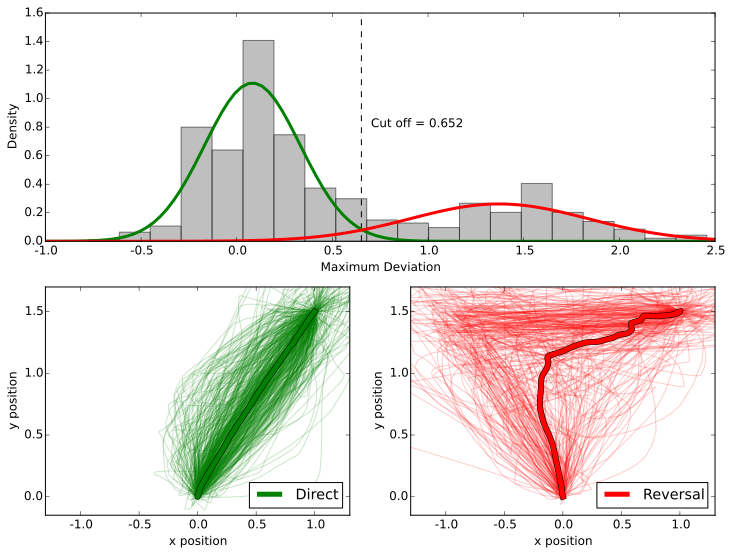
\includegraphics[width=\textwidth]{imgs/reversals/exp1-reversals}
  \caption[]{
    \label{fig:exp1-reversals}
    Trajectories classed as direct and reversals in Experiment 1.
  }
\end{figure}

Bimodality Coefficient = 0.689.
Hartigan's' D = 0.027, N = 580, p = 0.006.

\begin{table}[hp]
  \centering
  \caption[]{
    Mean and SD, and relative proportions, of the Maximum Deviation for direct and reversal trials, in Experiment 1
    \label{tab:appendix-reversals-1}
  }
  \begin{tabular}{lrr}
    \toprule
                       &   Direct &   Reversal \\
    \midrule
    Mean               &     0.08 &             1.37 \\
    Standard deviation &     0.25 &             0.46 \\
    Proportion         &    70\%    &            30\%    \\
    \bottomrule
  \end{tabular}
  
\end{table}


\newpage
\FloatBarrier
\section*{Experiment 2}\label{experiment-2}

\begin{figure}[ht]
  \centering
  \includegraphics[width=\textwidth]{imgs/reversals/exp2-reversals}
  \caption[]{
    \label{fig:exp2-reversals}
    Trajectories classed as direct and reversals in Experiment 2.
  }
\end{figure}


Bimodality Coefficient = 0.65.
Hartigan's' D = 0.021, N = 754, p = .0182.

\begin{table}[hp]
  \centering
  \caption[]{
    Mean and SD, and relative proportions, of the Maximum Deviation for direct and reversal trials, in Experiment 2
    \label{tab:appendix-reversals-2}
  }
  \begin{tabular}{lrr}
    \toprule
    &   Direct &   Reversal \\
    \midrule
    Mean               &     0.13 &             1.39 \\
    Standard deviation &     0.26 &             0.42 \\
    Proportion         &    64\%    &            36\%    \\
    \bottomrule
  \end{tabular}
\end{table}


\newpage
\FloatBarrier
\section*{Experiment 3}\label{experiment-3}

\begin{figure}[ht]
  \centering
  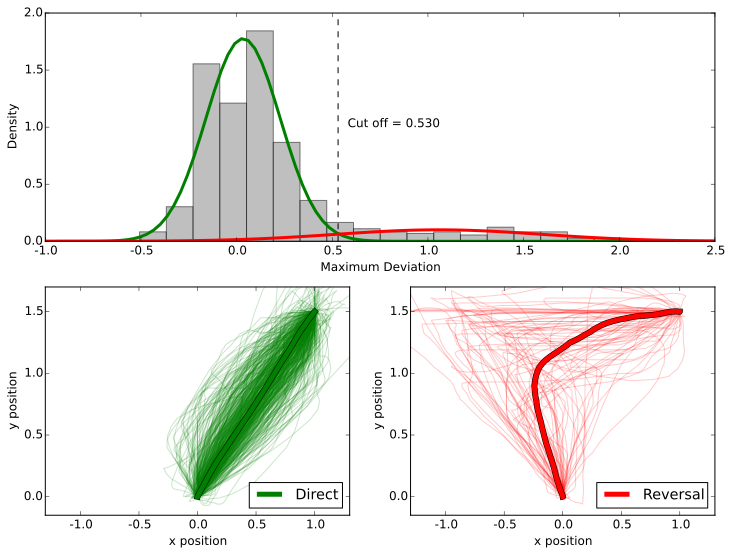
\includegraphics[width=\textwidth]{imgs/reversals/exp3-reversals}
  \caption[]{
    \label{fig:exp3-reversals}
    Trajectories classed as direct and reversals in Experiment 3
    (after data was excluded from stimulus sets for which participants
    performed poorly on the post-test check; see Chapter 4).
  }
\end{figure}


Bimodality Coefficient = 0.705.
Hartigan's' D = 0.042, N = 520, p < .0001.


\begin{table}[hp]
  \centering
  \caption[]{
    Mean and SD, and relative proportions, of the Maximum Deviation for direct and reversal trials, in Experiment 3
    \label{tab:appendix-reversals-3}
  }
  \begin{tabular}{lrr}
    \toprule
    &   Direct &   Reversal \\
    \midrule
    Mean               &     0.03 &             1.06 \\
    Standard deviation &     0.19 &             0.54 \\
    Proportion         &    86\%    &            14\%    \\
    \bottomrule
  \end{tabular}
\end{table}

\newpage
\FloatBarrier
\section*{Experiment 4}\label{experiment-4}

\begin{figure}[ht]
  \centering
  \includegraphics[width=\textwidth]{imgs/reversals/exp4-reversals}
  \caption[]{
    \label{fig:exp4-reversals}
    Trajectories classed as direct and reversals in Experiment 4.
  }
\end{figure}


Bimodality Coefficient = 0.636.
Hartigan's' D = 0.025, N = 1188, p < .0001.

\begin{table}[hp]
  \centering
  \caption[]{
    Mean and SD, and relative proportions, of the Maximum Deviation for direct and reversal trials, in Experiment 4
    \label{tab:appendix-reversals-4}
  }
  \begin{tabular}{lrr}
    \toprule
    &   Direct &   Reversal \\
    \midrule
    Mean               &     0.12 &             1.43 \\
    Standard deviation &     0.31 &             0.32 \\
    Proportion         &    77\%    &            23\%    \\
    \bottomrule
  \end{tabular}
\end{table}

\newpage
\FloatBarrier
\section*{Experiment 5}\label{experiment-5}

\begin{figure}[ht]
  \centering
  \includegraphics[width=\textwidth]{imgs/reversals/exp5-reversals}
  \caption[]{
    \label{fig:exp5-reversals}
    Trajectories classed as direct and reversals in Experiment 5.
  }
\end{figure}

Bimodality Coefficient = 0.562.
Hartigan's' D = 0.024, N = 1998, p < .0001.

\begin{table}[hp]
  \centering
  \caption[]{
    Mean and SD, and relative proportions, of the Maximum Deviation for direct and reversal trials, in Experiment 1
    \label{tab:appendix-reversals-5}
  }
  \begin{tabular}{lrr}
    \toprule
    &   Direct &   Reversal \\
    \toprule
    Mean               &     0.07 &             1.4  \\
    Standard deviation &     0.39 &             0.34 \\
    Proportion         &    66\%    &            34\%    \\
    \toprule
  \end{tabular}
\end{table}

  
  %% Chapter 3
  \chapter{Stimuli from Experiment 1}\label{appendix:exp1_stimuli}
    %% http://tex.stackexchange.com/a/88939/60964
  % \centering
  %%   \hspace*{-2cm} \begin{tabular}{rcccc}
  %%   \toprule
  %%   Set & Base species                     & Correct option                & Conflict foil                 & Control foil \\
  %%   \midrule
  %%   1   & \smallpic{imgs/bird}             & \smallpic{imgs/flamingo}      & \smallpic{imgs/bat}           & \smallpic{imgs/fox}          \\
  %%   2   & \smallpic{imgs/dandelions}       & \smallpic{imgs/roses}         & \smallpic{imgs/coral_flower}  & \smallpic{imgs/coral_brain}  \\
  %%   3   & \smallpic{imgs/bug_leafy}        & \smallpic{imgs/bug_ladybird}  & \smallpic{imgs/plant_leaf}    & \smallpic{imgs/tree_winter}  \\
  %%   4   & \smallpic{imgs/hedgehog}         & \smallpic{imgs/dog}           & \smallpic{imgs/pinecone}      & \smallpic{imgs/sycamore}     \\
  %%   5   & \smallpic{imgs/dino_triceratops} & \smallpic{imgs/dino_sauropod} & \smallpic{imgs/rhino}         & \smallpic{imgs/cat}          \\
  %%   \bottomrule
  %% \end{tabular}\hspace*{-2cm}
  \vspace*{-2cm}\begin{longtable}{rcccc}
    \caption[]{ Stimulus images used in Experiment 1.} \label{} \\
    
    \toprule
    Set & Base species                     & Correct option                & Conflict foil                 & Control foil \\
    \midrule
    \endfirsthead

    \toprule
    Set & Base species                     & Correct option                & Conflict foil                 & Control foil \\
    \midrule
    \endhead

    %% \hline \multicolumn{3}{|r|}{{Continued on next page}} \\ \hline
    \bottomrule
    \endfoot
    
    \bottomrule
    \bottomrule
    \endlastfoot

    1   & \smallpic{imgs/exp1/bird}             & \smallpic{imgs/exp1/flamingo}      & \smallpic{imgs/exp1/bat}           & \smallpic{imgs/exp1/fox}          \\
    2   & \smallpic{imgs/exp1/dandelions}       & \smallpic{imgs/exp1/roses}         & \smallpic{imgs/exp1/coral_flower}  & \smallpic{imgs/exp1/coral_brain}  \\
    3   & \smallpic{imgs/exp1/bug_leafy}        & \smallpic{imgs/exp1/bug_ladybird}  & \smallpic{imgs/exp1/plant_leaf}    & \smallpic{imgs/exp1/tree_winter}  \\
    4   & \smallpic{imgs/exp1/hedgehog}         & \smallpic{imgs/exp1/dog}           & \smallpic{imgs/exp1/pinecone}      & \smallpic{imgs/exp1/sycamore}     \\
    5   & \smallpic{imgs/exp1/dino_triceratops} & \smallpic{imgs/exp1/dino_sauropod} & \smallpic{imgs/exp1/rhino}         & \smallpic{imgs/exp1/cat}          \\
    6   & \smallpic{imgs/exp1/tuna}             & \smallpic{imgs/exp1/fish_yellow}   & \smallpic{imgs/exp1/dolphin}       & \smallpic{imgs/exp1/badger}       \\
    7   & \smallpic{imgs/exp1/lime}             & \smallpic{imgs/exp1/strawberry}    & \smallpic{imgs/exp1/fish_green}    & \smallpic{imgs/exp1/mackerel}     \\
    8   & \smallpic{imgs/exp1/duck}             & \smallpic{imgs/exp1/eagle}         & \smallpic{imgs/exp1/platypus}      & \smallpic{imgs/exp1/kangaroo}     \\
    9   & \smallpic{imgs/exp1/leopard}          & \smallpic{imgs/exp1/deer}          & \smallpic{imgs/exp1/leopard_gecko} & \smallpic{imgs/exp1/gecko}        \\
    10  & \smallpic{imgs/exp1/fish_stripey}     & \smallpic{imgs/exp1/goldfish}      & \smallpic{imgs/exp1/zebra}         & \smallpic{imgs/exp1/horse}       \\
    
\end{longtable}\vspace*{-2cm}
  %% \caption[]{}


  \chapter{Post test scores for stimuli used in Experiment 1} \label{appendix:exp1_posttest}
  \begin{table}[h!]
  \centering
  \begin{tabular}{rrr}
    \toprule
    Base                  &  Correct response  (Accuracy)   & Conflict foil       (Accuracy)   \\
    \midrule                                                                                     
    Bird                   & Flamingo           (92\%)  & Bat                  (85\%) \\
    Dandelions             & Roses              (98\%)  & Coral (flower-like)  (82\%) \\
    Insect (leaf-like)     & Insect (Ladybird)  (93\%)  & Plant (leafy)        (100\%)\\
    Hedgehog               & Dog                (87\%)  & Pinecone             (100\%)\\
    Dinosaur (Triceratops) & Dinosaur (Sauropod) (91\%)  & Rhino                (68\%) \\
    Tuna                   & Fish (yellow)      (95\%)  & Dolphin              (71\%) \\
    Lime                   & Strawberry         (100\%) & Fish (green)         (100\%)\\
    Duck                   & Eagle              (92\%)  & Platypus             (73\%) \\
    Leopard                & Deer               (95\%)  & Leopard Gecko        (97\%) \\
    Fish (stripey)         & Goldfish           (100\%) & Zebra                (95\%) \\
    \bottomrule
  \end{tabular}
  \caption[]{
    Accuracy on the post-test for stimuli pairs used in Experiment 1.
    Scores greater than 67.8\% are significant at the p < .01 level.
    }
\end{table}



  \chapter{Stimuli from Experiment 2}\label{appendix:exp2_stimuli}
  
\begin{table}[!h]
  \centering
  \caption[]{
    Stimuli used in Experiment 3:
    animals called Flurps, and robots called Floobits.
    There were four possible colourations, and four possible body shapes,
    and each colouration and body shape was equally likely to occur in each category.
    Categories could be recognised by inspecting their heads.
  }
  \hspace*{-1cm}\begin{tabular}{llll}
    \toprule\toprule
    \multicolumn{4}{c}{Flurps}\\
    \midrule
    \pic{imgs/exp2/AA4.jpg} &
    \pic{imgs/exp2/AB3.jpg} &
    \pic{imgs/exp2/AC2.jpg} &
    \pic{imgs/exp2/AD1.jpg} \\
    \toprule
    \multicolumn{4}{c}{Floobits}\\
    \midrule
    \pic{imgs/exp2/WA1.jpg} &
    \pic{imgs/exp2/WB2.jpg} &
    \pic{imgs/exp2/WC3.jpg} &
    \pic{imgs/exp2/WD4.jpg} \\
    \bottomrule\bottomrule
  \end{tabular}\hspace*{-1cm}
\end{table}


  \chapter{Properties used in Experiment 2}\label{appendix:exp2_properties}
  
Properties were presented in the form ``This one X. Who else do you think X''.

\textbf{Properties specific to Flurps (animals)}

\begin{itemize} 
  \singlespacing
    \item This one breathes. 
    \item This one can have babies. 
    \item This one has a heart inside. 
    \item This one has a mummy. 
    \item This one has bones inside. 
    \item This one needs water. 
    \item This one can climb trees. 
    \item This one tries to stay warm. 
\end{itemize}

\textbf{Properties specific to Floobits (robots)}
\begin{itemize}
\singlespacing
    \item This one can be turned off. 
    \item This one can break. 
    \item This one has batteries inside. 
    \item This one has wires inside. 
    \item This one was made by people. 
    \item This one was sold in a store. 
    \item This one is cold touch. 
    \item This one doesn't sleep. 
\end{itemize}

\textbf{Generic properties}
\begin{itemize}
\singlespacing
    \item This one can make a zevy sound. 
    \item This one has a very sticky toma. 
    \item This one has zimmer inside. 
    \item This one is used for derriping. 
    \item This one needs tiddles to make it move. 
    \item This one uses danner. 
    \item This one can help yippets. 
    \item This one goes outside in the winter. 
    \item This one has a part inside called a cece. 
    \item This one has blickets inside of it. 
    \item This one has grumpets that make it strong. 
    \item This one is good for kertling. 
    \item This one is found on farms. 
    \item This one can be very old. 
    \item This one feels yinty. 
    \item This one lacks ombelots. 
\end{itemize}




  %% Chapter 4
  \chapter{Association ratings for stimuli used in Experiment 3}\label{appendix:exp3_associations}
  
\begin{table}[hb]
  \centering
  \caption[]{
    Experimental stimulus sets from Experiment 3.
    Values in parentheses denote mean strength of association
    between that species and the base species,
    on a scale from 1 to 9, as collected by \citet{Crisp-Bright2010}.
  }
  \label{tbl:crisp-stimuli}
  \begin{tabular}{lrrr}
    \toprule
    Base        & Correct response & Conflict foil      & Control foil\\
    \midrule
    Acorns      & Lychees (3.7)     & Squirrels (7.9)     & Seals\\
    Butterflies & Locusts (5.5)     & Flowers (7.6)       & Seaweed\\
    Ants        & Dragonflies (4.5) & Anteaters (7.6)     & Moose\\
    Grass       & Palm Trees (5.0)  & Sheep (7.5)         & Hyenas\\
    Carrots     & Bamboo (3.1)      & Rabbits (7.7)       & Tigers\\
    Shepherds   & Bus Drivers (3.3) & Sheep (8.2)         & Porpoises\\
    Orca Whales & Cows (2.2)        & Cod (5.3)           & Pigeons\\
    Snails      & Octopuses (2.8)   & Hedgehogs (4.3)     & Sloths\\
    Salmon      & Goldfish (5.0)    & Grizzly Bears (7.5) & Hedgehogs\\
    Monkeys     & Seals (2.5)       & Peanuts (6.8)       & Almonds\\
    Bananas     & Tulips (2.4)      & Monkeys (7.5)       & Sea Lions\\
    Mice        & Goats (2.7)       & Wheat (4.4)         & Bamboo\\
    Penguins    & Chickens (3.0)    & Orca Whales (5.9)   & Dogs\\
    Dolphins    & Llamas (2.0)      & Cod (7.3)           & Parrots\\
    \bottomrule
  \end{tabular}
\end{table}

  \chapter{Stimuli used in Experiment 3}\label{appendix:exp3_stimuli}
  
\begin{table} [H]
  %% http://tex.stackexchange.com/a/88939/60964
  \caption[]{
    Stimulus images used in Experiment 3.
  }
  \centering
    \hspace*{-2cm} \begin{tabular}{rcccc}
    \toprule
    Set & Base species                & Correct option              & Conflict foil             & Control foil \\
    \midrule
    1   & \smallpic{imgs/exp3/Acorns}      & \smallpic{imgs/exp3/Lychees}     & \smallpic{imgs/exp3/Squirrels} & \smallpic{imgs/exp3/Seals} \\ 
    2   & \smallpic{imgs/exp3/Butterflies} & \smallpic{imgs/exp3/Locusts}     & \smallpic{imgs/exp3/Flowers}   & \smallpic{imgs/exp3/Seaweed} \\
    3   & \smallpic{imgs/exp3/Ants}        & \smallpic{imgs/exp3/Dragonflies} & \smallpic{imgs/exp3/Anteaters} & \smallpic{imgs/exp3/Moose} \\ 
    4   & \smallpic{imgs/exp3/Grass}       & \smallpic{imgs/exp3/Palm_trees}  & \smallpic{imgs/exp3/Sheep}     & \smallpic{imgs/exp3/Hyenas} \\ 
    5   & \smallpic{imgs/exp3/Carrots}     & \smallpic{imgs/exp3/Bamboo}      & \smallpic{imgs/exp3/Rabbits}   & \smallpic{imgs/exp3/Tigers} \\ 
    \bottomrule
    \end{tabular}\hspace*{-2cm}
  %% \caption[]{}
\end{table}

\begin{table} [h!]
  %% http://tex.stackexchange.com/a/88939/60964
  \centering
    \hspace*{-4cm} \begin{tabular}{rcccc}
    \toprule
    Set & Base species                  & Correct option                      & Conflict foil                      & Control foil \\
    \midrule
    6   & \smallpic{imgs/exp3/Shepherds}   & \smallpic{imgs/exp3/Bus_drivers} & \smallpic{imgs/exp3/Sheep}     & \smallpic{imgs/exp3/Porpoises} \\
    7   & \smallpic{imgs/exp3/Orca} & \smallpic{imgs/exp3/Cows}        & \smallpic{imgs/exp3/Cod}       & \smallpic{imgs/exp3/Pigeons} \\
    8   & \smallpic{imgs/exp3/Snails}   &      \smallpic{imgs/exp3/Octopuses} &   \smallpic{imgs/exp3/Hedgehogs}   &     \smallpic{imgs/exp3/Sloths}	\\  
    9   & \smallpic{imgs/exp3/Salmon}   &      \smallpic{imgs/exp3/Goldfish}  &    \smallpic{imgs/exp3/Bears}      & \smallpic{imgs/exp3/Hedgehogs}	\\
    10  & \smallpic{imgs/exp3/Monkeys}  &     \smallpic{imgs/exp3/Seals}      &       \smallpic{imgs/exp3/Peanuts} &       \smallpic{imgs/exp3/Almonds}	\\
    11  & \smallpic{imgs/exp3/Bananas}  &     \smallpic{imgs/exp3/Tulips}     &      \smallpic{imgs/exp3/Monkeys}  &       \smallpic{imgs/exp3/Sealions}	\\
    12  & \smallpic{imgs/exp3/Mice}     &        \smallpic{imgs/exp3/Goats}   &       \smallpic{imgs/exp3/Wheat}   &         \smallpic{imgs/exp3/Bamboo}	\\  
    13  & \smallpic{imgs/exp3/Penguins} &    \smallpic{imgs/exp3/Chickens}    &    \smallpic{imgs/exp3/Orca}       &   \smallpic{imgs/exp3/Dogs}	\\  
    14  & \smallpic{imgs/exp3/Dolphins} &    \smallpic{imgs/exp3/Llamas}      &      \smallpic{imgs/exp3/Cod}      &           \smallpic{imgs/exp3/Parrots}	\\ 
    \bottomrule
  \end{tabular}\hspace*{-4cm}
  %% \caption[]{}
\end{table}




  \chapter{Post test performance for stimuli used in Experiment 3}\label{appendix:exp3_posttest}
  \begin{table}[!h]
  \centering
  \caption[]{
    Participants' accuracy on the post-test check in Experiment 3, for each stimulus set.
    Participants were significantly above chance at correctly identifying that
    the base and correct response species belonged to the same taxonomic group
    for seven of the fourteen stimulus sets (left column),
    and at correctly identifying that the base and foil species
    did not belong to the same group for eleven of fourteen sets.
  }
  \label{tbl:exp3-post}
  \begin{tabular}{lPP}
    \toprule
    Base        & \multicolumn{1}{r}{Correct species} & \multicolumn{1}{r}{Foil species}\\
    \midrule
    Dolphins    & 40\%           & 65\% \\
    Monkeys     & 40.3\%         & 97.2\% ^{**}\\
    Snails      & 42.6\%         & 89.7\% ^{**}\\
    Bananas     & 52.9\%         & 97.1\% ^{**}\\
    Penguins    & 53\%           & 57.6\%\\
    Mice        & 56.5\%         & 97.1\% ^{**}\\
    Orca        & 60\%           & 66.2\% \\
    Acorns      & 81.1\% ^{**} & 98.6\% ^{**}\\
    Butterflies & 85.9\% ^{**} & 90.1\% ^{**}\\
    Carrots     & 90.1\% ^{**} & 100\% ^{**}\\
    Ants        & 93\% ^{**}   & 93\% ^{**}\\
    Grass       & 100\% ^{**}  & 97.1\% ^{**}\\
    Salmon      & 100\% ^{**}  & 98.6\% ^{**}\\
    Shepherds   & 100\% ^{**}  & 82.6\% ^{**}\\
    \bottomrule
    \multicolumn{3}{l}{
      \emph{Note}: $^{**}p < .01.$
    }
  \end{tabular}
\end{table}

  \chapter{Stimuli used in Experiment 4}\label{appendix:exp4_stimuli}
  
%% \rotatebox{90}{
%%   %% http://tex.stackexchange.com/a/88939/60964
%%   \centering
%%   \begin{tabular}{rccccc}
%%     \toprule
%%     Set & Base species                      & Correct option                    & Weak foil                       & Moderate foil                  & Strong foil \\
%%     \midrule
%%     1   &\sidewayssmallpic{imgs/exp4/acorns}        & \sidewayssmallpic{imgs/exp4/strawberries} & \sidewayssmallpic{imgs/exp4/cats}       & \sidewayssmallpic{imgs/exp4/chipmunks} & \sidewayssmallpic{imgs/exp4/squirrels} \\
%%     2   &\sidewayssmallpic{imgs/exp4/ants}          & \sidewayssmallpic{imgs/exp4/butterflies}  & \sidewayssmallpic{imgs/exp4/dogs}       & \sidewayssmallpic{imgs/exp4/aardvarks} & \sidewayssmallpic{imgs/exp4/anteaters} \\
%%     3   &\sidewayssmallpic{imgs/exp4/bears}         & \sidewayssmallpic{imgs/exp4/hamsters}     & \sidewayssmallpic{imgs/exp4/clownfish}  & \sidewayssmallpic{imgs/exp4/trout}     & \sidewayssmallpic{imgs/exp4/salmon} \\
%%     4   &\sidewayssmallpic{imgs/exp4/carrots}       & \sidewayssmallpic{imgs/exp4/bamboo}       & \sidewayssmallpic{imgs/exp4/foxes}      & \sidewayssmallpic{imgs/exp4/horses}    & \sidewayssmallpic{imgs/exp4/rabbits} \\
%%     5   &\sidewayssmallpic{imgs/exp4/grass}         & \sidewayssmallpic{imgs/exp4/oranges}      & \sidewayssmallpic{imgs/exp4/mosquitoes} & \sidewayssmallpic{imgs/exp4/beetles}   & \sidewayssmallpic{imgs/exp4/crickets} \\
%%     6   &\sidewayssmallpic{imgs/exp4/killer_whales} & \sidewayssmallpic{imgs/exp4/hippos}       & \sidewayssmallpic{imgs/exp4/goldfish}   & \sidewayssmallpic{imgs/exp4/cod}       & \sidewayssmallpic{imgs/exp4/sharks} \\
%%     7   &\sidewayssmallpic{imgs/exp4/mice}          & \sidewayssmallpic{imgs/exp4/camels}       & \sidewayssmallpic{imgs/exp4/emus}       & \sidewayssmallpic{imgs/exp4/kestrels}  & \sidewayssmallpic{imgs/exp4/owls} \\
%%     \bottomrule
%%   \end{tabular}
%%   }

\setlength\LTleft{-0.4cm}
\setlength\LTright{-0.4cm}

\begin{center}
  \small
  \begin{longtable}{L{.02\textwidth} L{.165\textwidth} L{.165\textwidth} L{.165\textwidth} L{.165\textwidth} L{.165\textwidth} }
    \caption[]{Stimulus images for experimental trials, Experiment 4.}\\
    \toprule
    & Base species                         & Correct option                       & Weak foil                          & Moderate foil                         & Strong foil \\
    \midrule
    \endfirsthead
    \endhead                                                                                                                                      \\
    \bottomrule
    \endfoot                                                                                                                                         \\

    1   &\onefifthpic{imgs/exp4/acorns}        & \onefifthpic{imgs/exp4/strawberries} & \onefifthpic{imgs/exp4/cats}       & \onefifthpic{imgs/exp4/chipmunks}     & \onefifthpic{imgs/exp4/squirrels} \\
    2   &\onefifthpic{imgs/exp4/ants}          & \onefifthpic{imgs/exp4/butterflies}  & \onefifthpic{imgs/exp4/dogs}       & \onefifthpic{imgs/exp4/aardvarks}     & \onefifthpic{imgs/exp4/anteaters} \\
    3   &\onefifthpic{imgs/exp4/bears}         & \onefifthpic{imgs/exp4/hamsters}     & \onefifthpic{imgs/exp4/clownfish}  & \onefifthpic{imgs/exp4/trout}         & \onefifthpic{imgs/exp4/salmon} \\
    4   &\onefifthpic{imgs/exp4/carrots}       & \onefifthpic{imgs/exp4/bamboo}       & \onefifthpic{imgs/exp4/foxes}      & \onefifthpic{imgs/exp4/horses}        & \onefifthpic{imgs/exp4/rabbits} \\
    5   &\onefifthpic{imgs/exp4/grass}         & \onefifthpic{imgs/exp4/oranges}      & \onefifthpic{imgs/exp4/mosquitoes} & \onefifthpic{imgs/exp4/beetles}       & \onefifthpic{imgs/exp4/crickets} \\
    6   &\onefifthpic{imgs/exp4/killer_whales} & \onefifthpic{imgs/exp4/hippos}       & \onefifthpic{imgs/exp4/goldfish}   & \onefifthpic{imgs/exp4/cod}           & \onefifthpic{imgs/exp4/sharks} \\
    7   &\onefifthpic{imgs/exp4/mice}          & \onefifthpic{imgs/exp4/camels}       & \onefifthpic{imgs/exp4/emus}       & \onefifthpic{imgs/exp4/kestrels}      & \onefifthpic{imgs/exp4/owls} \\
    8   &\onefifthpic{imgs/exp4/owls}          & \onefifthpic{imgs/exp4/chickens}     & \onefifthpic{imgs/exp4/llamas}     & \onefifthpic{imgs/exp4/foxes}         & \onefifthpic{imgs/exp4/bats} \\
    9   &\onefifthpic{imgs/exp4/penguins}      & \onefifthpic{imgs/exp4/robins}       & \onefifthpic{imgs/exp4/goats}      & \onefifthpic{imgs/exp4/arctic_wolves} & \onefifthpic{imgs/exp4/polar_bears} \\
  \end{longtable}
\end{center}

\setlength\LTleft{0cm}
\setlength\LTright{0cm}

\FloatBarrier


\begin{table}[!h]
  \centering
  \caption[]{Stimulus sets for experimental trials, Experiment 4.
    \label{tbl:exp4-species}
  }
  \begin{tabular}{lllll}
    \toprule
    Base          & Correct species  & Weak foil  & Moderate foil & Strong foil        \\
    \midrule
    Acorns        & Strawberries     & Cats       & Chipmunks     & Squirrels    \\
    Ants          & Butterflies      & Dogs       & Aardvarks     & Anteaters    \\
    Bears         & Hamsters         & Clownfish  & Trout         & Salmon        \\
    Carrots       & Bamboo           & Foxes      & Horses        & Rabbits      \\
    Grass         & Oranges          & Mosquitoes & Beetles       & Crickets     \\
    Killer Whales & Hippos           & Goldfish   & Cod           & Sharks       \\
    Mice          & Camels           & Emus       & Kestrels      & Owls         \\
    Owls          & Chickens         & Llamas     & Foxes         & Bats         \\
    Penguins      & Robins           & Goats      & Arctic Wolves & Polar Bears  \\
    \bottomrule
  \end{tabular}
\end{table}





%% 4   &\smallpic{imgs/exp4/carrots}       & \smallpic{imgs/exp4/bamboo}       & \smallpic{imgs/exp4/foxes}      & \smallpic{imgs/exp4/horses}    & \smallpic{imgs/exp4/rabbits} \\






  \chapter{Post test performance for stimuli used in Experiment 4} \label{appendix:exp4_posttest}
  
\begin{table}[!h]
  \centering
  \caption[]{
    Performance on the post-test for each stimulus set from Experiment 4.
    Participants successfully identified that the correct response species
    belonged to the same taxonomic group as the base,
    and that the two foil species presented did not,
    on at least 70\% of trials (p's < .01).
  }
  \begin{tabular}{lrrr}
    \toprule
    %% Base          & Correct species      \\
    %% \midrule                              
    %% Acorns        & Strawberries (95\%)  \\
    %% Ants          & Butterflies (93\%)   \\
    %% Bears         & Hamsters (91\%)      \\
    %% Carrots       & Bamboo (89\%)        \\
    %% Grass         & Oranges (91\%)       \\
    %% Killer Whales & Hippos (70\%$^{\*}$) \\
    %% Mice          & Camels (86\%)        \\
    %% Owls          & Chickens (84\%)      \\
    %% Penguins      & Robins (84\%)        \\
    Base          & Correct Species      & Foil \#1           & Foil \#2 \\
    \midrule
    Acorns        & Strawberries (95\%)  & Chipmunks (98\%)   & Squirrels (95\%)\\
    Ants          & Butterflies (93\%)   & Aardvarks (91\%)   & Anteaters (86\%)\\
    Bears         & Hamsters (91\%)      & Salmon (89\%)      & Trout (93\%)\\
    Carrots       & Bamboo (89\%)        & Horses (84\%)      & Rabbits (95\%)\\
    Grass         & Oranges (91\%)       & Crickets (98\%)    & Beetles (95\%)\\
    Killer Whales & Hippos (70\%$^{\*}$) & Cod (91\%)         & Sharks (100\%)\\
    Mice          & Camels (86\%)        & Kestrels (95\%)    & Owls (95\%)\\
    Owls          & Chickens (84\%)      & Bats (93\%)        & Foxes (75\%)\\
    Penguins      & Robins (84\%)        & Polar bears (91\%) & Arctic wolves (91\%)\\
    \bottomrule
    \multicolumn{2}{l}{
      \emph{Note:} $^*$ p < .01; All other p's < .0001.
      }
  \end{tabular}
\end{table}



  
  %% Chapter 5
  \chapter{Bayesian model priors from Experiment 5}\label{appendix:exp5_bayes}
  \begin{equation}
  \begin{split}
    log(\ rt_{(p,\ d)}\ ) &=  (\Alpha + \alpha_p + \alpha_d)
    + Condition * \Beta + \epsilon \\
    \Alpha &\sim Uniform(0, 8.5) \\
    \Beta &\sim Normal(-.69, .69) \\
    \alpha_p &\sim Normal(0, \sigma_{\alpha_p}) \\
    \alpha_d &\sim Normal(0, \sigma_{\alpha_d}) \\
    \sigma^2_{\alpha_P} &\sim Cauchy(0, 10); \sigma^2_{\alpha_P} > 0 \\
    \sigma^2_{\alpha_D} &\sim Cauchy(0, 10); \sigma^2_{\alpha_D} > 0
  \end{split}
\end{equation}

This model predicts log response time ($rt$)
for participants $p$, reasoning about description $d$.
The model parameters are the overall intercept term $\Alpha$,
representing the log of the average response time when
the base rates agreed with the description,
participant $p$'s offset from this intercept, $\alpha_p$,
and description $d$'s offset, $\alpha_d$
--- both of which were normally distributed with a mean of 0,
the regression weight $\Beta$,
representing the log of the percentage increase in $rt$ when the base rate disagrees,
and the error term $\epsilon$.
$Condition$ is 0 for trials where the cues agree,
and 1 where they disagree.
A uniform prior was  set on $\Alpha$ so that
all baseline $rt$s from 1 to 5,000 msec were equally likely.
$\Beta$ was give a broad normal prior with mean 0 and SD .69,
meaning that, a priori, I was 95\% certain that
response times would be between 5 times slower and 5 times faster
than those when the cues agreed.
The variance parameters for the
by-participant and by-description differences in the intercept
had uninformative half-Cauchy distributions,
indicating that I could not specify in advance
how much variance there would be \citep{Gelman2006b}.

  
  %% Chapter 6
  \chapter{CRT Reasoning Problems from Experiment 6}\label{appendix:exp6_stimuli}
  \begin{center}
  \singlespacing
  \begin{longtable}{llrrlrr}
    \caption[]{
      Stimuli used in Experiment 6.
      Items 1--3 were adapted from \citet{Frederick2005}.
      Items 4--8 were adapted from \citet{Primi2015}.
      \emph{Note.} Percentages in parentheses show the proportion of participants who gave each response.
    }\\
    \toprule
    & \multicolumn{3}{l}{Conflict} & \multicolumn{3}{l}{No-conflict} \\
    \midrule
    \endfirsthead
    \toprule
    & \multicolumn{3}{l}{Conflict} & \multicolumn{3}{l}{No-conflict} \\
    \midrule
    \endhead

    \bottomrule
    \endfoot

    \bottomrule\bottomrule
    \endlastfoot

    1 &
    \multicolumn{3}{ p{.4\textwidth} }{
      A bat and a ball together costs £1.10.
      A bat costs £1 more than a ball.
      How~much~does~a~ball~cost?}
    & \multicolumn{3}{ p{.4\textwidth} }{
      A bat and a ball together costs £1.05.
      A bat costs £1.
      How much does a ball cost?
    } \\*
    \\*
    & Correct response:   & 5p   &(15\%) &  Correct response:  & 5p & (97\%)\\*
    & Heuristic response: & 10p   &(83\%) &  Foil response:     & 10p & (0\%)\\*
    & Foil response:      & 15p   &(0\%)  &  Foil response:    & 15p & (1\%)\\*
    & Foil response:      & 90p   &(2\%)  &  Foil response:    & 90p & (1\%)\\
    \midrule

    2 &
    \multicolumn{3}{ p{.4\textwidth} }{
      It takes 5 machines 5 minutes to make 5 
      widgets. How many minutes would it take 100
      machines to make 100 widgets?}
    & \multicolumn{3}{ p{.4\textwidth} }{
      It takes a machine 5 minutes to make 5 
      widgets. How many minutes would it take the
      machines to make 100 widgets?
    } \\*
    \\*
    & Correct response:   & 5   &(24\%) &  Correct response:  & 100 & (83\%)\\*
    & Heuristic response: & 100   &(69\%) &  Foil response:     & 5 & (2\%)\\*
    & Foil response:      & 50   &(4\%)  &  Foil response:    & 50 & (13\%)\\*
    & Foil response:      & 10   &(3\%)  &  Foil response:    & 10 & (2\%)\\
    \midrule

    3 &
    \multicolumn{3}{ p{.4\textwidth} }{
      In a lake, there is a patch of lily pads.
      Every day, the patch doubles in size.
      If it takes 48 days for the patch to cover
      the entire lake, how many days would it take
      for the patch to cover half of the lake?}
    & \multicolumn{3}{ p{.4\textwidth} }{
      In a lake, there is a patch of lily pads.
      Every day, the patch grows by 10m².
      If it takes 48 days for the patch to cover
      the 150m², how many days would it take
      for the patch to cover 140m²?
    } \\*
    \\*
    & Correct response:   & 47   &(25\%) &  Correct response:  & 47 & (79\%)\\*
    & Heuristic response: & 24   &(59\%) &  Foil response:     & 24 & (17\%)\\*
    & Foil response:      & 12   &(15\%)  &  Foil response:    & 12 & (4\%)\\*
    & Foil response:      & 2   &(2\%)  &  Foil response:    & 2 & (0\%)\\
    \bottomrule

    4 &
    \multicolumn{3}{ p{.4\textwidth} }{
      If you flipped a fair coin twice, what is
      the probability that it would land
      'Heads' at least once?}
    & \multicolumn{3}{ p{.4\textwidth} }{
      If you flipped a fair coin twice, what is
      the probability that it would land
      'Heads' exactly once?
    } \\*
    \\*
    & Correct response:   & 75\%   &(4\%) &  Correct response:  & 25\% & (68\%)\\*
    & Heuristic response: & 50\%   &(84\%) &  Foil response:     & 50\% & (26\%)\\*
    & Foil response:      & 25\%   &(11\%)  &  Foil response:    & 75\% & (6\%)\\*
    & Foil response:      & 100\%   &(1\%)  &  Foil response:    & 100\% & (0\%)\\
    \midrule

    5 &
    \multicolumn{3}{ p{.4\textwidth} }{
      If 3 elves can wrap 3 toys in
      1 hour, how many elves are needed
      to wrap 6 toys in 2 hours?}
    & \multicolumn{3}{ p{.4\textwidth} }{
      If 3 elves can wrap 3 toys in
      1 hour, how many toys could 6 elves
      wrap in half an hour?
    } \\*
    \\*
    & Correct response:   & 3   &(73\%) &  Correct response:  & 3 & (71\%)\\*
    & Heuristic response: & 6   &(22\%) &  Foil response:     & 6 & (20\%)\\*
    & Foil response:      & 1   &(2\%)  &  Foil response:    & 1 & (1\%)\\*
    & Foil response:      & 12   &(4\%)  &  Foil response:    & 12 & (8\%)\\*
    \midrule

    6 &
    \multicolumn{3}{ p{.4\textwidth} }{
      Ellen and Kim are running around a track.
      They run equally fast but Ellen started later.
      When Ellen has run 5 laps, Kim has run 10 laps.
      When Ellen has run 10 laps, how many has Kim run?}
    & \multicolumn{3}{ p{.4\textwidth} }{
      Ellen and Kim are running around a track.
      They started at the same time,
      but Kim is twice as fast as Ellen.
      When Ellen has run 5 laps, Kim has run 10 laps.
      When Ellen has run 10 laps, how many has Kim run?
    } \\*
    \\*
    & Correct response:   & 15   &(73\%) &  Correct response:  & 20 & (98\%)\\*
    & Heuristic response: & 20   &(27\%) &  Foil response:     & 15 & (2\%)\\*
    & Foil response:      & 5   &(0\%)  &  Foil response:    & 5 & (0\%)\\*
    & Foil response:      & 19   &(0\%)  &  Foil response:    & 19 & (0\%)\\
    \midrule

    7 &
    \multicolumn{3}{ p{.4\textwidth} }{
      Jerry received both the 15th highest and
      the 15th lowest mark in the class. How many
      students are there in the class?}
    & \multicolumn{3}{ p{.4\textwidth} }{
      Jerry received both the 2nd highest and
      the 2nd lowest mark in the class. How many
      students are there in the class?
    } \\*
    \\*
    & Correct response:   & 29   &(26\%) &  Correct response:  & 3 & (79\%)\\*
    & Heuristic response: & 30   &(72\%) &  Foil response:     & 2 & (13\%)\\*
    & Foil response:      & 40   &(2\%)  &  Foil response:    & 5 & (8\%)\\*
    & Foil response:      & 5   &(0\%)  &  Foil response:    & 10 & (0\%)\\
    \midrule

    8 &
    \multicolumn{3}{ p{.4\textwidth} }{
      In an athletics team tall members tend to win
      three times as many medals than short members.
      This year the team has won 60 medals so far.
      How many of these have been won by short athletes?}
    & \multicolumn{3}{ p{.4\textwidth} }{
      In an athletics team tall members tend to win
      twice as many medals than short members.
      This year the team has won 60 medals so far.
      How many of these have been won by short athletes?
    } \\*
    \\*
    & Correct response:   & 15   &(44\%) &  Correct response:  & 20 & (58\%)\\*
    & Heuristic response: & 20   &(52\%) &  Foil response:     & 15 & (12\%)\\*
    & Foil response:      & 30   &(1\%)  &  Foil response:    & 30 & (27\%)\\*
    & Foil response:      & 50   &(3\%)  &  Foil response:    & 50 & (4\%)\\
  \end{longtable}
\end{center}

%% \begin{table}[!h]
%%   \centering
%%   \caption[]{
%%     Stimuli used in Experiment 6.
%%     Items 1--3 were adapted from \citet{Frederick2005}.
%%     Items 4--8 were adapted from \citet{Primi2015}.
%%     \emph{Note.} Percentages in parentheses show the proportion of participants who gave each response.
%%   }
%%   \singlespacing
%%   \footnotesize
%%   \begin{tabular}{llrrlrr}
%%     \toprule
%%     & \multicolumn{3}{l}{Conflict} & \multicolumn{3}{l}{No-conflict} \\
%%     \midrule

%%     %% \parbox[b]{2mm}{\multirow{6}{*}{\rotatebox[origin=c]{90}{1. Bat-and-ball}}} &
%%     1 &
%%     \multicolumn{3}{ p{.4\textwidth} }{
%%       A bat and a ball together costs £1.10.
%%       A bat costs £1 more than a ball.
%%       How~much~does~a~ball~cost?}
%%     & \multicolumn{3}{ p{.4\textwidth} }{
%%       A bat and a ball together costs £1.05.
%%       A bat costs £1.
%%       How much does a ball cost?
%%     } \\
%%     \\
%%     & Correct response:   & 5p   &(15\%) &  Correct response:  & 5p & (97\%)\\*
%%     & Heuristic response: & 10p   &(83\%) &  Foil response:     & 10p & (0\%)\\*
%%     & Foil response:      & 15p   &(0\%)  &  Foil response:    & 15p & (1\%)\\*
%%     & Foil response:      & 90p   &(2\%)  &  Foil response:    & 90p & (1\%)\\*
%%     \midrule

%%     2 &
%%     \multicolumn{3}{ p{.4\textwidth} }{
%%       It takes 5 machines 5 minutes to make 5 
%%       widgets. How many minutes would it take 100
%%       machines to make 100 widgets?}
%%     & \multicolumn{3}{ p{.4\textwidth} }{
%%       It takes a machine 5 minutes to make 5 
%%       widgets. How many minutes would it take the
%%       machines to make 100 widgets?
%%     } \\
%%     \\
%%     & Correct response:   & 5   &(24\%) &  Correct response:  & 100 & (83\%)\\*
%%     & Heuristic response: & 100   &(69\%) &  Foil response:     & 5 & (2\%)\\*
%%     & Foil response:      & 50   &(4\%)  &  Foil response:    & 50 & (13\%)\\*
%%     & Foil response:      & 10   &(3\%)  &  Foil response:    & 10 & (2\%)\\*
%%     \midrule

%%     3 &
%%     \multicolumn{3}{ p{.4\textwidth} }{
%%       In a lake, there is a patch of lily pads.
%%       Every day, the patch doubles in size.
%%       If it takes 48 days for the patch to cover
%%       the entire lake, how many days would it take
%%       for the patch to cover half of the lake?}
%%     & \multicolumn{3}{ p{.4\textwidth} }{
%%       In a lake, there is a patch of lily pads.
%%       Every day, the patch grows by 10m².
%%       If it takes 48 days for the patch to cover
%%       the 150m², how many days would it take
%%       for the patch to cover 140m²?
%%     } \\
%%     \\
%%     & Correct response:   & 47   &(25\%) &  Correct response:  & 47 & (79\%)\\*
%%     & Heuristic response: & 24   &(59\%) &  Foil response:     & 24 & (17\%)\\*
%%     & Foil response:      & 12   &(15\%)  &  Foil response:    & 12 & (4\%)\\*
%%     & Foil response:      & 2   &(2\%)  &  Foil response:    & 2 & (0\%)\\*
%%     \bottomrule
%%   \end{tabular}
%% \end{table}

%% \begin{table}
%%   \centering
%%   \footnotesize
%%   \begin{tabular}{llrrlrr}
%%     \toprule
%%     & \multicolumn{3}{l}{Conflict} & \multicolumn{3}{l}{No-conflict} \\
%%     \midrule

%%     4 &
%%     \multicolumn{3}{ p{.4\textwidth} }{
%%       If you flipped a fair coin twice, what is
%%       the probability that it would land
%%       'Heads' at least once?}
%%     & \multicolumn{3}{ p{.4\textwidth} }{
%%       If you flipped a fair coin twice, what is
%%       the probability that it would land
%%       'Heads' exactly once?
%%     } \\
%%     \\
%%     & Correct response:   & 75\%   &(4\%) &  Correct response:  & 25\% & (68\%)\\*
%%     & Heuristic response: & 50\%   &(84\%) &  Foil response:     & 50\% & (26\%)\\*
%%     & Foil response:      & 25\%   &(11\%)  &  Foil response:    & 75\% & (6\%)\\*
%%     & Foil response:      & 100\%   &(1\%)  &  Foil response:    & 100\% & (0\%)\\*    
%%     \midrule

%%     5 &
%%     \multicolumn{3}{ p{.4\textwidth} }{
%%       If 3 elves can wrap 3 toys in
%%       1 hour, how many elves are needed
%%       to wrap 6 toys in 2 hours?}
%%     & \multicolumn{3}{ p{.4\textwidth} }{
%%       If 3 elves can wrap 3 toys in
%%       1 hour, how many toys could 6 elves
%%       wrap in half an hour?
%%     } \\
%%     \\
%%     & Correct response:   & 3   &(73\%) &  Correct response:  & 3 & (71\%)\\*
%%     & Heuristic response: & 6   &(22\%) &  Foil response:     & 6 & (20\%)\\*
%%     & Foil response:      & 1   &(2\%)  &  Foil response:    & 1 & (1\%)\\*
%%     & Foil response:      & 12   &(4\%)  &  Foil response:    & 12 & (8\%)\\*
%%     \midrule

%%     6 &
%%     \multicolumn{3}{ p{.4\textwidth} }{
%%       Ellen and Kim are running around a track.
%%       They run equally fast but Ellen started later.
%%       When Ellen has run 5 laps, Kim has run 10 laps.
%%       When Ellen has run 10 laps, how many has Kim run?}
%%     & \multicolumn{3}{ p{.4\textwidth} }{
%%       Ellen and Kim are running around a track.
%%       They started at the same time,
%%       but Kim is twice as fast as Ellen.
%%       When Ellen has run 5 laps, Kim has run 10 laps.
%%       When Ellen has run 10 laps, how many has Kim run?
%%     } \\
%%     \\
%%     & Correct response:   & 15   &(73\%) &  Correct response:  & 20 & (98\%)\\*
%%     & Heuristic response: & 20   &(27\%) &  Foil response:     & 15 & (2\%)\\*
%%     & Foil response:      & 5   &(0\%)  &  Foil response:    & 5 & (0\%)\\*
%%     & Foil response:      & 19   &(0\%)  &  Foil response:    & 19 & (0\%)\\*
%%     \midrule

%%     7 &
%%     \multicolumn{3}{ p{.4\textwidth} }{
%%       Jerry received both the 15th highest and
%%       the 15th lowest mark in the class. How many
%%       students are there in the class?}
%%     & \multicolumn{3}{ p{.4\textwidth} }{
%%       Jerry received both the 2nd highest and
%%       the 2nd lowest mark in the class. How many
%%       students are there in the class?
%%     } \\
%%     \\
%%     & Correct response:   & 29   &(26\%) &  Correct response:  & 3 & (79\%)\\*
%%     & Heuristic response: & 30   &(72\%) &  Foil response:     & 2 & (13\%)\\*
%%     & Foil response:      & 40   &(2\%)  &  Foil response:    & 5 & (8\%)\\*
%%     & Foil response:      & 5   &(0\%)  &  Foil response:    & 10 & (0\%)\\*
%%     \midrule

%%     8 &
%%     \multicolumn{3}{ p{.4\textwidth} }{
%%       In an athletics team tall members tend to win
%%       three times as many medals than short members.
%%       This year the team has won 60 medals so far.
%%       How many of these have been won by short athletes?}
%%     & \multicolumn{3}{ p{.4\textwidth} }{
%%       In an athletics team tall members tend to win
%%       twice as many medals than short members.
%%       This year the team has won 60 medals so far.
%%       How many of these have been won by short athletes?
%%     } \\
%%     \\
%%     & Correct response:   & 15   &(44\%) &  Correct response:  & 20 & (58\%)\\*
%%     & Heuristic response: & 20   &(52\%) &  Foil response:     & 15 & (12\%)\\*
%%     & Foil response:      & 30   &(1\%)  &  Foil response:    & 30 & (27\%)\\*
%%     & Foil response:      & 50   &(3\%)  &  Foil response:    & 50 & (4\%)\\*

%%     \bottomrule
%%   \end{tabular}
%% \end{table}


  
\end{appendices}

\end{document}
